\documentclass[a4paper]{article}
%% Language and font encodings
\usepackage[english]{babel}
\usepackage[utf8x]{inputenc}
\usepackage[T1]{fontenc}
\usepackage{float}
%% Sets page size and margins
\usepackage[a4paper,top=3cm,bottom=2cm,left=3cm,right=3cm,marginparwidth=1.75cm]{geometry}
\usepackage[caption=false]{subfig}
%% Useful packages
\usepackage{fancyhdr}
\pagestyle{fancy}
\usepackage{amsmath}
\usepackage{amsthm}
\usepackage{enumitem}
\usepackage{eqnarray}
\usepackage{float}
\usepackage{esint}
\usepackage{wrapfig}
\usepackage{gensymb}
\usepackage{lipsum}
\usepackage{amssymb}
\usepackage{array}
\usepackage{tikz}
\usepackage[colorlinks=true, allcolors=blue]{hyperref}
\usepackage{graphicx}
\usepackage{amsmath}
\usepackage{amssymb}
\usepackage{graphicx}
\usepackage{mathtools}
\usepackage[colorlinks=true, allcolors=blue]{hyperref}
\DeclareMathOperator{\lcm}{lcm}
\DeclareMathOperator{\var}{Var}
\DeclareMathOperator{\cov}{Cov}
\DeclareMathOperator{\sgn}{sgn}
\DeclareMathOperator{\Span}{span}
\DeclareMathOperator{\nullity}{nullity}
\DeclareMathOperator{\rank}{rank}
\DeclareMathOperator{\Ker}{Ker}
\DeclareMathOperator{\R}{R}
\DeclareMathOperator{\Tr}{Tr}
\DeclareMathOperator{\sinc}{sinc}
\DeclareMathOperator{\diag}{diag}
\newtheorem{defi}{Definition}[section]
\newtheorem{remarks}{Remarks}[section]
\newtheorem{note}{Note}[section]
\newtheorem{law}{Law}[section]
\newtheorem{eg}{Example}[section]
\newtheorem{notation}{Notation}[section]
\newtheorem{thm}{Theorem}[section]
\newtheorem{prop}{Proposition}[section]
\newtheorem{lemma}{Lemma}[section]
\newtheorem{cor}{Corollary}[section]

\definecolor{darkblue}{RGB}{	0, 0, 139}
\newtheoremstyle{new}% <name>
{5pt}% <Space above>
{5pt}% <Space below>
{\color{black}}% Body font
{}% <Indent amount>
{\bfseries\color{darkblue}}% Theorem head font
{:}% <Punctuation after theorem head>
{.5em}% <Space after theorem headi>
{}% <Theorem head spec (can be left empty, meaning `normal')>
\theoremstyle{new}
\newtheorem{Note}{Note}[section]

\title{\textbf{Part 1B Physics A Summary Notes}}
\author{Tai Yingzhe, Tommy (ytt26)}
\date{}
\setlength{\parindent}{0cm}
\begin{document}
\maketitle
\tableofcontents
\newpage
\section{Experimental Methods}
Suggested booklist: \cite{ahmed_spreadbury_1984, 10.5555/2960712,squires_2001,dunlap1988experimental,hughes2010measurements}
\subsection{Understanding your Experiment}
\subsubsection*{Measurement in Physics}
\begin{Note}[Idea of Experimental Physics]
Experimental physics is about devising measurements, making these measurements and assessing the results using statistical models. Typically, by changing a quantity in the system, an effect is induced (which we need to track these changes conveniently). This is measured by a device/transducer (ideally does not perturb the system) and subsequently handle the signal and record the data. Laboratory work may serve
\begin{itemize}
    \item to demonstrate theoretical ideas in physics - for teaching purposes. 
    \item to provide a familiarity with apparatus - training for laboratory work.
    \item to provide a training in how to do experiments - plan, eliminate errors, analyze result, estimate accuracy, record measurements and calculations accurately, clearly and concisely.
\end{itemize}
\end{Note}
\begin{Note}[Technique to measure frequency]
The phenomenon of beats provides a very precise method of measuring the frequency $f$ of a source, particularly for EM waves. Mixing this with a standard source whose frequency is known very precisely $f_0$, we then obtain a beat waveform, allowing us to measure the beat frequency $f_b$, i.e. $f=f_0\pm f_b$.~\cite{squires_2001}
\end{Note}
\begin{Note}[Technique to measure electric signals]
Nowadays, \textbf{data taking are mostly computerized} and our data is (indirectly) in the form of electrical signals. In particular, these measurements may be very small and one has to amplify them to bring them into a measurable range, without corrupting them.\\[5pt]
Input and output impedances are very important in measuring. Ideally, we want \textbf{input impedance to be very high}, i.e. draw as little current as possible. Also, we want \textbf{low output impedance} such that source provides as much current as possible. Oscilloscope is excellent in measuring the voltage profile against time. The transducer part is an equivalent Thevenin circuit with an output impedance in series with the output voltage. The scope part is an equivalent Norton circuit with an input impedance parallel to the input voltage. As a consequence of current conservation, we have $V_{in}=V_{out}\frac{Z_{in}}{Z_{in}+Z_{out}}$, by the potential divider rule.\\[5pt]
In reality, $Z_{in}$ is complex, which poses a problem at high frequencies. This can be compensated using scope probes via $C_{in}R_{in}=C_{probe}R_{probe}$ but as a result, $V_{out}\neq V_{in}$.\\[5pt]
For current measurements, you least disturb the system if the measurement device takes all of the current, i.e. low $Z_{in}$. To transfer maximum power from one system to another, $Z_{out}$ of one system is equal to $Z_{out}$ of another. The high $Z_{in}$ of a scope is great for measuring voltage signals but little power gets into the oscilloscope, hence motivating the use of operational amplifiers - \textbf{packaged, high gain, high input impedance, voltage amplifier}.
\end{Note}
\begin{Note}[Power Matching]
Power matching is used mainly in 3 situations:
\begin{itemize}
    \item where the signal levels are very small so \textbf{any power lost gives a much worse signal-to-noise ratio};
    \item where the signal at high frequency is connected through \textbf{lines of appreciable self-capacity and self-inductance} to a load. Then it is possible to get \textbf{large standing waves due to reflections from the load} which can make the source-to-load power transfer low;
    \item where signals are very large, say at the output stage of a transmitter, and where the \textbf{maximum efficiency is desirable on economic ground}s.
\end{itemize}
\end{Note}
\newpage
\begin{Note}[Terminology for Pulse]
For a train of pulse, the voltage is switched from a low state ($V_1$) to a high state ($V_2$), so $V_2-V_1$ is the amplitude. The \textbf{pulse duration} is the time for which the pulse is at level $V_2$. The ratio of time for which the pulse is high to that for low is called the \textbf{mark-to-space ratio}, i.e. $\frac{t_2-t_1}{t_3-t_1}$. The \textbf{duty cycle} is the time for which the pulse is high in a period. The \textbf{repetition frequency} of a pulse train is the number of pulses per second, i.e. $\frac{1}{t_2-t_1}$ Hz. A \textbf{rise time} is defined as time in which pulse voltage rises from 10 percent to 90 percent. Similarly, a decay time can be defined, which may not necessarily be equal for a given pulse. Time constant, $\tau$, is the time to rise to $(1-e^{-1})V_1\approx0.63V_1$.~\cite{ahmed_spreadbury_1984}
\end{Note}
\begin{Note}[Feedback]
Suppose we have an electronic amplifier which has the property that, when a voltage $V_i$ is applied across its input terminals, a voltage $V_o$ appears across its output terminals, where $V_o=\alpha V_i$, where $\alpha$ is the intrinsic gain of the amplifier.\\[5pt]
Suppose now that we have a certain signal voltage $V_s$ that we wish to amplify, but that, instead of applying $V_s$ directly to the input terminals, we subtract from it a fraction $\beta V_o$ of the output and apply the remainder to the input terminals. This is known as negative feedback. 
$$V_i=V_s-\beta V_o\implies V_o=\alpha(V_s-\beta V_o)\implies\frac{V_s}{V_o}=\frac{\alpha}{1+\alpha\beta}$$
\textbf{The net overall gain is reduced by the feedback}. When $\alpha\beta>>1$, the gain becomes $1/\beta$, \textbf{independent of the intrinsic gain} (open-loop gain), but inversely proportional to the fraction of the output being fed back. \textbf{Advantages} are:
\begin{itemize}
    \item Insensitivity to variations in high voltage and amplifier components
    \item Improved frequency response for sinusoidal inputs. 
    \item Improved linearity: $V_o$ is approximately a linear function of $V_s$, regardless of how non-linear the relation between $V_o$ and $V_i$.
    \item Input impedance of amplifier is increased and its output impedance decreased.
\end{itemize}
If sign of the feedback signal is reversed, i.e. $\beta<0$, we will have positive feedback. When $V_o$ become so large, the capacitive and inductive elements give time delays and the system begins to oscillate. Such circuits are designed to function as oscillators. Even if we intend to only achieve negative feedback, positive feedback may occur at certain frequencies. This is because the amplifier produces phase shifts in the signals and these shifts depend on frequency.~\cite{ahmed_spreadbury_1984,10.5555/2960712}
\end{Note}
\begin{Note}[Filters]
There are two types of filters: passive filters and active filters. Latter is distinguished by their presence of operational amplifiers. For filters, the \textbf{ratio of input to output voltage is generally quoted as decibels}. For the first-order low-pass filter, at $\omega=\frac{1}{RC}$, we have $20\log(2^{-1/2})$ which is $-3$dB. The \textbf{amount by which the output has decreased is called rolloff}. The rolloff is generally measured in dB per \textbf{octave} (a factor of 2 in frequency) or \textbf{decade} (a factor of 10 in frequency). Two problems that arise in passive filters can be solved easily with op-amps:~\cite{ahmed_spreadbury_1984,10.5555/2960712}
\begin{itemize}
    \item the dependence of the filter characteristics on the input and output impedance;
    \item the attenuation of the signal due to impedance of the filter
\end{itemize}
\end{Note}
\newpage
\subsubsection*{Theory of Ideal Operational Amplifiers (Op-Amp)~\cite{ahmed_spreadbury_1984}}
\begin{defi}[Gain]
Gain is the \textbf{ratio between output voltage to input voltage}. This is usually frequency-dependent, but might be constant in the mid-band (between two frequencies). For operational amplifiers (op-amps), there will come a time when $X_o$ cannot rise any more, even as $X_i$ is increased, due to the limitations of the supply, i.e. \textbf{saturation}.
\end{defi}
\begin{defi}[Power Gain]
The power gain, measured in decibels dB, is defined to be
$$10\log_{10}\frac{P_o}{P_i}=20\log_{10}\frac{V_o}{V_i}$$
\end{defi}
\begin{Note}[Utility of Decibel Unit]
Decibel units are \textbf{useful} for two reasons:
\begin{itemize}
    \item Response curves of many circuits have simple forms when the gain in decibels is plotted against the frequency on a logarithmic scale;
    \item when amplifiers are followed by further circuits with gain ($+$ dB) or attenuation ($-$ dB), then the overall gain is obtained algebraically by summing the gains and attenuations of all parts in a path between the input and output.
\end{itemize}
\end{Note}
\begin{defi}[Operational Amplifier]
An operational amplifier (op-amp) is a \textbf{DC-coupled high-gain electronic voltage amplifier with a differential input} and, usually, a \textbf{single-ended output}. We have $V_{out}=A(V_+-V_-)$ where $A$ is the no-load voltage gain, $V_+$ and $V_-$ are the voltages at the (+) and (-) terminals respectively. There is a difference between \textbf{common-mode signal input} (identical signals applied to both (-) and (+) terminals) and \textbf{differential-mode signal input}. The former has zero output while the latter has large output signal.\\[5pt]
The problem arise when a tiny $V_{in}$ makes $V_{out}=\infty$, exceeding the $\pm15$ V (finite power supply) supply limit and thus lead to saturation. We can \textbf{control the gain by using negative feedback}, i.e. feed some output back into negative output to prevent output from saturating.
\end{defi}
\begin{Note}[Ideal Op-Amp]
Ideally, one assumes that the operational amplifier has \textbf{infinitely high input impedance} and a \textbf{zero output impedance} (device can supply arbitrary large currents and still maintain prescribed value of $V_{out}$). Often, it might also be required that these properties be \textbf{maintained over a particular frequency range} or at least be true, to a close approximation, at a specified operating frequency, i.e. infinite gain with zero phase shift at all frequencies (\textbf{purely real}). Furthermore, there \textbf{should be no upper limit on the magnitude of the output voltage}, i.e. no clipping.\\[5pt]
With infinitely high $Z_{in}$, we have the current drawn into the (-) terminal to be approximately zero, $I_-\approx 0$. If $V_+$ is connected to earth, we have $V_-\approx 0$, and hence $V_-\approx V_+$. Hence, the \textbf{golden rules} (\textbf{valid only for negative feedback} ideal operational amplifiers, such that we achieve stable self-consistent solutions) are
\begin{enumerate}
    \item Input draws no current, since $Z_{in}$ is infinity.
    \item Voltages on $+$ and $-$ inputs are the same, unless output is saturated since $A$ is so high.
\end{enumerate}
\end{Note}
\begin{eg}[Inverting Amplifier]
The input signal is applied to the ($-$) terminal via a resistance $R_1$ often called the input resistor and the ($+$) terminal is connected to the common rail, therefore no signal voltage appears at the input. The amplifier output is fed back to the ($-$) terminal via $R_2$, called the feedback resistor. With the Golden rules, we have at the node X, $i_1=-i_2$ since $Z_{in}$ is infinite, hence $i_-=0$. We thus have $\frac{v_1-0}{R_1}=\frac{0-v_2}{R_2}\implies\frac{v_2}{v_1}=-\frac{R_2}{R_1}$.
\end{eg}
\begin{eg}[Non-Inverting Amplifier]
The signal is applied to the ($+$) terminal but the circuit connection using $R_2$ and $R_1$ are still made to the ($-$) terminal. One end of $R_1$ is joined to Earth. Let $v'$ be the voltage at the inverting input, then we have $v_2=A(v_1-v')$, then
$$v'=\frac{R_1}{R_1+R_2}v_2\implies\frac{v_2}{v_1}=\frac{A}{1+A\frac{R_1}{R_1+R_2}}\approx1+\frac{R_2}{R_1}$$
for very large $A$.
\end{eg}
\begin{eg}[Differential Amplifier]
The basic property is to amplify the difference between the two input signals. We let the potentials $v_1'$ and $v_2'$ to be the voltage at nodes X and Y respectively. Assuming ideal, (-) terminal draws no current, and so does (+) terminal since $V_-=V_+$, we have
$$\frac{v_1-v_1'}{R_1}=\frac{v_1'-v_3}{R_2}$$
$$\frac{v_2-v_2'}{R_3}=\frac{v_2'}{R_4}$$
and given $A(v_2'-v_1')=v_3$, we then have $v_3=\frac{R_2}{R_1}(v_2-v_1)$ where we set $\frac{R_4}{R_3}=\frac{R_2}{R_1}$ and assuming $A$ very large.
\end{eg}
\begin{figure}[H]
    \centering
    \includegraphics[scale=0.65]{invertingideal.PNG}
    \caption{Ideal Inverting Operational Amplifier. Figure from \cite{ahmed_spreadbury_1984}.}
    \label{invertingideal}
\end{figure}
\begin{figure}[H]
    \centering
    \includegraphics[scale=0.65]{non-invertingideal.PNG}
    \caption{Ideal Non-inverting Operational Amplifier. Figure from \cite{ahmed_spreadbury_1984}.}
\end{figure}
\begin{figure}[H]
    \centering
    \includegraphics[scale=0.65]{differentialideal.PNG}
    \caption{Ideal Differential Operational Amplifier. Figure from \cite{ahmed_spreadbury_1984}.}
\end{figure}
\begin{eg}[Voltage Follower]
Also known as a unity-gain buffer amplifier. Its voltage gain is very close to unity, and its main function is to \textbf{act as isolation between a signal generator and a load resistance}. This can be treated as a special case of the non-inverting amplifier such that $v_2=A(-v_2+v_1)\implies\frac{v_2}{v_1}=\frac{A}{A+1}\approx 1$ for very high $A$.
\end{eg}
\begin{figure}[H]
    \centering
    \includegraphics[scale=0.6]{bufferideal.PNG}
    \caption{Ideal voltage follower. Figure from \cite{ahmed_spreadbury_1984}.}
    \label{bufferideal}
\end{figure}
\begin{eg}[Integrator]
An operational amplifier with a capacitor in place of the resistance which usually links output to input acts as an integrating circuit. Assuming voltage $v'$ at node X and ideal conditions, we have
$$\frac{v_1-v'}{R_1}=i_1=i_2$$
Since $i_2$ flows through the capacitor $C_1$, we can write
$$v_2-v'=-\frac{1}{C_1}\int_0^ti_1dt$$
but $v'=-v_2/A$. When $A$ is very large, $v'\rightarrow0$, we thus have $v_2=-\frac{1}{R_1C_1}\int_0^tv_1dt$, i.e. the output is the integral of the input voltage $v_1$. \textbf{Assuming AC voltage of the exponential form}, we have $V_{out}=-\frac{1}{i\omega RC}|V_{in}|e^{i\omega t}$. Not only it performs integration in analogue computers, it amplifies signals of low frequencies $\omega$, and also inverts the input signal. \textbf{Possible problems at very low frequencies}, which can be resolved by adding a resistor parallel to the capacitor. Moreover, this operation is undefined for $\omega=0$, leading to \textbf{saturation}.
\end{eg}
\begin{figure}[H]
    \centering
    \includegraphics[scale=0.65]{integratingideal.PNG}
    \caption{Ideal Integrating Amplifier. Figure from \cite{ahmed_spreadbury_1984}.}
    \label{integratingideal}
\end{figure}
\begin{eg}[Differentiator]
The differentiating operational amplifier may be constructed by merely interchanging the positions of the capacitor and resistors of the integrator. The output is then (replace $v_1$ with $v_2$ in the previous result, and then differentiate the integral) $v_2=-R_1C_1\frac{d}{dt}v_1$. This circuit is however rarely used because it suffers from the \textbf{disadvantage that it amplifies noise and spurious voltage spikes at the input}. A \textbf{capacitor across $R_1$ can be used to minimize} this effect at the expense of exact differentiation.
\end{eg}
\begin{figure}[H]
    \centering
    \includegraphics[scale=0.65]{differentiatingideal.PNG}
    \caption{Ideal Differentiating Amplifier. Figure from \cite{ahmed_spreadbury_1984}.}
    \label{differentiatingideal}
\end{figure}
\begin{eg}[Simulating Inductance]
\textbf{Inductance is avoided in integrated circuit design because of technological difficulties}. One can simulate an inductance by using an R-C network in conjunction with the amplifier. For an ideal operational amplifier, we have the op-amp to behave like a buffer, i.e. $v_2=v'$. To sum the currents at node X, we have
$$i_1=i_2+i_3=\frac{v_1-v_2}{R_2}+\frac{v_1}{R_1+1/(i\omega C)}\implies\frac{v_1}{i_1}=\frac{R_1R_2^2\omega^2C^2+R_2}{1+\omega^2C^2R_2^2}+i\frac{\omega R_2C}{1+\omega^2C^2R_2^2}(R_1-R_2)$$
To appear as an inductor, we must have $R_1-R_2>0$. For $R_1>>R_2$, we have the \textbf{apparent inductance} to be $L\approx R_1R_2C$. It behaves like an inductor in the phase shift ($\pi/2$).
\end{eg}
\begin{figure}[H]
    \centering
    \includegraphics[scale=0.85]{simulatinginductance.PNG}
    \caption{Simulation of an inductance with an ideal operational amplifier. Figure from \cite{ahmed_spreadbury_1984}.}
    \label{simulatinginductance}
\end{figure}
\begin{eg}[Filter]
A band-pass filter must pass all signals over a range of frequency without attenuation or perhaps even with amplification. \textbf{All signals outside this range must be attenuated by as large a factor as possible}. It is possible to construct such a filter using \textbf{frequency selective feedback across an amplifier}. \textbf{Unwanted signals are fed back to keep the overall gain low while the wanted signals are not fed back}. A suitable frequency selective network is a twin-T network but it requires to have in it six carefully matched components to function well. A simpler circuit shown below uses only five components in addition to an ideal amplifier.\\[5pt]
The gain $\frac{v_2}{v_1}$ of the circuit may be determined by summing the currents at the node X, i.e. $$i_1+i_2+i_3=i_4\implies\frac{v_1-v_3}{R_1}+\frac{-v_2/A-v_3}{1/i\omega C_0}+\frac{v_2-v_3}{1/i\omega C_0}=\frac{v_3}{R_2}$$
We assume that $Z_{in}$ of the amplifier is very high as usual, so conserving current, $$i_5=i_2\implies\frac{v_2+v_2/A}{R_3}=\frac{-v_2/A-v_3}{1/i\omega C_0}$$ Expressing $v_3$ in terms of $v_2$ and assuming $v_2/A<<v_2$, we have $$v_3=\frac{iv_2}{\omega C_0R_3}-\frac{v_2}{A}$$
Substituting this into the current conservation, we have
$$\frac{v_2}{v_1}=-\frac{1}{R_1\bigg(\frac{2}{R_3}+\frac{1}{A}\bigg(\frac{1}{R_1}+\frac{1}{R_2}\bigg)\bigg)+iR_1\bigg(\frac{1/R_1+1/R_2}{\omega C_0R_3}-\omega C_0\bigg)}$$
The maximum gain is approximate to be $-\frac{R_3}{2R_1}$ (due to high $A$). This occurs at the frequency $\omega^2=\frac{1/R_1+1/R_2}{C_0^2R_3}$. Equating the real part to the imaginary part earlier, gives the half-power bandwidth $\Delta f=\frac{1}{\pi C_0R_3}$. 
\end{eg}

\begin{figure}[H]
    \centering
    \includegraphics{filter.PNG}
    \caption{A filter circuit with an ideal operational amplifier. Figure from \cite{ahmed_spreadbury_1984}.}
    \label{filter}
\end{figure}
\newpage
\subsubsection*{Theory of Non-Ideal Op-Amp~\cite{ahmed_spreadbury_1984}}
\begin{Note}[Non-Ideal Op-Amp]
$A$ is not infinity but is \textbf{finitely high}, of the magnitude $10^4$ to $10^6$. $A$ is a function of $\omega$, i.e. \textbf{complex}, hence giving a phase shift for certain frequencies. $Z_{in}$ is not infinite but finitely high, $Z_{out}$ not zero but low. There is also a \textbf{finite slew rate} $\frac{dV_{out}}{dt}$. There is also an \textbf{input bias current} independent of $V_{in}\sim10^{-12}$ to $10^{-7}$ A that sets an upper limit to external resistor values. There is an output voltage independent of $V_+-V_-$ (differential offset of $\sim10^{-3}$-$10^{-2}$V) balanced with an external potentiometer. Further, the output voltage is capped at some finite magnitude due to the finite power source of the amplifier, and hence exhibit \textbf{clipping}. 
\end{Note}
\begin{eg}[Non-Ideal Inverting]
We now assume input resistance $R_i$ and gain $A$ being finite (but high) and the output impedance $R_o$ to be non-zero. At node X, (feed back into ($-$) terminal)
$$\frac{v_1-v'}{R_1}+\frac{v_2-v'}{R_2}=\frac{v'}{R_i}$$
and at node Y,
$$\frac{v_0-v_2}{R_o}=\frac{v_2-v'}{R_2}$$
where $v_o=-Av'$ since ($+$) terminal is grounded. We thus have
$$\frac{v_1}{R_1}+\frac{v_2}{R_2}=v'\bigg(\frac{1}{R_i}+\frac{1}{R_1}+\frac{1}{R_2}\bigg),\frac{v_2}{R_2}+\frac{v_2}{R_o}=v'\bigg(\frac{1}{R_2}-\frac{A}{R_o}\bigg)$$
Eliminating $v'$, the gain will be
$$\frac{v_2}{v_1}=\frac{R_iR_o-AR_2R_i}{AR_1R_i+R_oR_1+R_oR_i+R_1R_2+R_1R_i+R_iR_2}$$
this reduces to the desired form if $A$ (more important) and $R_i$ are very large, i.e. $\frac{v_2}{v_1}\approx -\frac{R_2}{R_1}$.
\end{eg}
\begin{figure}[H]
    \centering
    \includegraphics[scale=0.9]{nonidealinverting.PNG}
    \caption{Non-ideal inverting amplifier, which includes input and output resistance.}
    \label{nonidealinverting}
\end{figure}
\newpage
\begin{eg}[Non-Ideal Non-Inverting]
Similarly, conserving currents at node X and Y, we have
$$\frac{v_2-v'}{R_2}=\frac{v'-v_1}{R_i}+\frac{v'}{R_1}$$
$$\frac{A(v_1-v')-v_2}{R_o}=\frac{v_2-v'}{R_2}+i_2$$
Eliminating $v'$ and simplifying, we have $v_2=v_1\mathcal{A}-i_2\mathcal{R}$ where
$$\mathcal{A}=\frac{R_oR_1+AR_i(R_2+R_1)}{R_i(R_1+R_2+AR_1)+R_1R_2+R_1R_o+R_iR_o}$$
is the no-load voltage gain (realistic) and
$$\mathcal{R}=\frac{R_o(R_iR_2+R_1R_2+R_1R_i)}{(1+R_o/R_2)(R_iR_2+R_1R_2+R_1R_i)+AR_iR_1-R_oR_1R_i/R_2}$$
When $A$ (more important) and $R_i$ are large, we have $\mathcal{A}\approx 1+\frac{R_2}{R_1}$ and $\mathcal{R}\approx\frac{R_o}{A}(1+\frac{R_2}{R_1})$ which is very small.
\end{eg}
\begin{figure}[H]
    \centering
    \includegraphics[scale=0.9]{nonidealnoninverting.PNG}
    \caption{Non-ideal non-inverting amplifier, which includes input and output resistance. Figure from \cite{ahmed_spreadbury_1984}.}
    \label{nonidealnoninverting}
\end{figure}
\newpage
\subsubsection*{Practical Considerations of Operational Amplifiers~\cite{ahmed_spreadbury_1984,10.5555/2960712}}
\begin{Note}[Frequency Response]
Many integrated circuit amplifiers behave like the following: the gain beyond the upper half power frequency decreases by 20 dB/decade (factor of 10) frequency rise.The typical frequency response is $A(f)=\frac{A_0}{1+i(f/f_0)}$ where $A_0$ is the gain of the internal amplifier at DC and low frequencies, and $f_0$ is the `turn over' frequency. We have 
$$A (dB)=20\log\frac{A_0}{\sqrt{1+(f/f_0)^2}}$$
with $\phi=-\tan^{-1}(f/f_0)$. Some, however, have faster rates of fall in frequency.\\[5pt]
$A$ will also \textbf{change with environmental conditions}, such as temperature. $A$ may also \textbf{fluctuate due to internal disturbance or supply variation}. Finally, $A$ itself may \textbf{depend on the input strength}, hence non-linear.
\end{Note}
\begin{Note}[Internal Frequency Compensation]
For finite $V_{out}$ below saturation, we have
$$V_{out}=|A(\omega)|e^{i\phi(\omega)}(V_+-V_-)$$
Since $\phi(\omega)\rightarrow\pi$ as $\omega$ approaches some critical frequency, the op-amp has an internal frequency compensation that \textbf{ensures the amplitude $A$ to fall off before the critical frequency}. This is to \textbf{prevent undesirable inter-conversion between positive and negative feedback}.
\end{Note}
\begin{Note}[Input Bias Currents and Input Offset Currents]
Operational amplifiers \textbf{draw small currents}, typically less than 1 $\mu$A, at the input terminals in order to bias the base or gate of the input transistors. The \textbf{effect of these bias currents is to produce a spurious output voltage when there is no input signal and the output should be zero or, in the presence of an input, an additional output is superimposed on the amplified signal}.\\[5pt]
Generally, this extra output is undesirable and it is particularly troublesome during operation in DC conditions. It is more significant when large resistors are used in the op-amp circuitry or the overall op-amp gain is high. The offset current is then defined to be the difference in input bias currents in the ($-$) and ($+$) terminals.
\end{Note}
\begin{Note}[Offset Voltage]
The \textbf{output voltage of an op-amp is not exactly zero} for another reason when there is no input signal and both the ($-$) and ($+$) inputs are earthed: steps must be taken to set the output to zero when there is no input signal. This offset voltage arises because the transistors in the differential amplifiers are not identical and other electronic circuitry in the integrated circuits is not perfectly balanced.\\[5pt]
The input offset voltage is defined as the small voltage needed at the input to make the output zero. The effect of the shift in the zero level can be a serious drawback since it \textbf{limits the maximum signal that may be handled without clipping one end of the waveform}.
\end{Note}
\begin{Note}[Common-Mode Rejection Ratio]
In real amplifiers, there will be a \textbf{small but finite gain for identical input signals}. We call such a gain to be the common-mode gain $A_{cm}$. We thus want to set this gain to be as small as possible. When expressed as the ratio $A/A_{cm}$, this is called the common-mode rejection ratio.
\end{Note}
\begin{Note}[Slewing Rate]
The behaviour of the operational amplifier\textbf{ when handling large signal inputs is not the same as when handling small signal inputs at the same frequency}. This is expressed by the slewing rate of the amplifier, which is the \textbf{maximum rate of change of the output voltage when the amplifier is supplying its rated output}. If the ideal output is a step, then the true output is a ramp with a  time $\Delta t$ to change the voltage b $\Delta V$. This ratio $\Delta V/\Delta t$ is the slewing rate and is given in $V/\mu s$. The effect is a function of the finite charging time of capacitors used in the operational amplifier's internal circuit and the load conditions.
\end{Note}
\newpage
\begin{Note}[Internal Gain Roll-off]
An internal roll-off of the \textbf{open-loop gain $A$ at very low frequencies} is typically introduced. This is to make sure that \textbf{parasitic capacitances both inside and outside the device do not lead to unstable condition}. This roll off is only noticeable in the closed-loop gain of the circuit as a whole when the open-loop gain becomes sufficiently small that the behavior of the op-amp cannot be adequately described by the Golden Rules.
\end{Note}
\subsubsection*{Feedback~\cite{ahmed_spreadbury_1984}}
\begin{defi}[Feedback]
Feedback is the process by which a fraction of the output signal, either a voltage or a current, is used as an input. It occurs in every system. If the feedback is undesired, then the input and output circuits of a system must be well separated and screened.\\[5pt]
Feedback reduces the overall gain of a system with the degree of reduction being related to the systems open-loop gain. Negative feedback also has effects of reducing distortion, noise, sensitivity to external changes as well as improving system bandwidth and input and output impedances.
\end{defi}
\begin{defi}[Feedback Circuit]
A feedback circuit is one where part of the output signal is added to the input. It can be added so as
\begin{itemize}
    \item to reduce the input - such feedback is then called negative feedback
    \item to increase the input - such feedback is then called positive feedback.
\end{itemize}
Consider some input signal $X_1$, applied to the system. If the amplifier has gain $A$, then for an output signal $X_2$, the required input is $X_2/A$. The amplifier is assumed to be unilateral and unaffected by the feedback circuit, B, which samples its output. The signal $X_2$ applied to the feedback circuit, B gives a signal B$X_2$ to be mixed with the input. At the input to the system, the signals are mixed, such that $\frac{X_2}{A}=X_1-BX_2\implies \frac{X_2}{X_1}=\frac{A}{1+AB}$, where $A$ is the forward gain and $AB$ is the loop gain. $\frac{A}{1+AB}$ is the overall gain of the system.\\[5pt]
Trivially, when there is no feedback, i.e. $B=0$, then the overall gain is just $A$. If either $A$ or $B$ is negative, $1+AB<1$ and so the overall gain is much greater than $A$, i.e. positive feedback. If $AB=-1$, then the overall gain is infinity. Further, if $A$ and $B$ are both positive or both negative, then $AB>>1$ and so the overall gain is $1/B$.
\end{defi}
\begin{Note}[Stabilization of Gain]
Suppose $A$, the gain of an amplifier without feedback, varies due to changes of supply voltage or circuit ambient temperature. How much does $K$, the gain feedback, vary? If we differentiate $K=\frac{A}{1+AB}$ with respect to $A$.
$$\frac{dK}{dA}=\frac{1+AB-AB}{(1+AB)^2}=\frac{1}{(1+AB)^2}\implies\frac{dK}{K}=\frac{(dA/A)}{1+AB}$$
With feedback, \textbf{a high, but relatively unstable gain can be traded for a lower gain and good stability} (less sensitive to environmental change). For example, if the amplifier (with gain 0.2) forward gain drops by 10 percent, then the change in overall gain is 0.05 percent.
\end{Note}
\begin{Note}[Disturbance in Amplifier]
'Disturbance' can be taken to mean any unwanted signal in the amplifier. It can be from poorly filtered supplies, thermal e.m.f.s in the circuit, Johnson noise in the circuit, or even non-linearity in the amplifier when the output is no longer directly related to the input. To generalize the analysis, let the disturbance to be between the input and the output of the amplifier such that the total forward gain is $A_1A_2$. The output signal $X_2=A_2(A_1(X_1-BX_2)+D)$, which is rearranged to
$$X_2=X_1\frac{A_1A_2}{1+A_1A_2B}+\frac{DA_2}{1+A_1A_2B}$$
We see that the disturbance $DA_2$ is reduced by the factor $1+A_1A_2B$. When $A_1A_2B>>1$, $X_2=\frac{X_1}{B}+\frac{D}{A_1B}$. The signal has been improved relative to the disturbance, assuming $A_1$ is noise-free amplification.
\end{Note}
\begin{eg}
When we need an amplifier of several stages to get a high forward gain $A$ before feedback, then we have a choice of how we may apply feedback to improve the amplifier's performance. Either we can apply some feedback across each stage or we can put it in one loop across the whole amplifier.\\[5pt]
Let arrangement (a) be the multi-stage amplifier with each stage having a forward gain of $A$. $B_1$ is the feedback required on each stage to get an overall gain $K_1$. The arrangement (b) is to put all the amplifiers in cascade when they will have a gain of $A^n$, and then to apply some different overall feedback $B_2$, to get the overall gain $K_2$. We have $K_1=\frac{A^n}{(1+AB_1)^n}$ and $K_2=\frac{A^n}{1+A^nB_2}$. The fractional gain changes will be $\frac{dK_1}{K_1}=\frac{n}{1+AB_1}\frac{dA}{A}$ and $\frac{dK_2}{K_2}=\frac{n}{1+A^nB_2}\frac{dA}{A}$. For the two circuits to have the same gain, we must have $K_1=K_2\implies(1+AB_1)^n=1+A^nB_2$, and hence
$$\frac{dK_2/K_2}{dK_1/K_1}=\frac{1}{(1+AB_1)^{n-1}}$$
For $n>1$ and with $1+AB_1$ large, then $\frac{dK_2}{K_2}<\frac{dK_1}{K_1}$. Thus overall feedback would appear to be beneficial as far as stabilizing the gain is concerned.
\end{eg}
\begin{Note}[Requirement for Oscillation]
The two conditions are:
\begin{itemize}
    \item the \textbf{magnitude of the gain round the loop shall be 1} to maintain oscillations;
    \item the \textbf{phase shift round the loop shall be 180 degrees} different from the condition normally required for negative feedback.
\end{itemize}
The feedback can also be applied to the other input of the differential amplifier. Qualitatively, if a signal exists at the output such that after being fed back through B and amplified by A it arrives back exactly with the same amplitude, so $|AB|=1$ and with the same phase, then it will be maintained and the circuit will be a generator.\\[5pt]
Further, in the design of a sinusoidal oscillator, two performance features need to be stable and well-defined: (a) the frequency, and (b) the amplitude of the signal generated.
\end{Note}
\begin{figure}[H]
    \centering
    \includegraphics[scale=0.75]{oscillator.PNG}
    \caption{Oscillates if (a) $A$ and $B$ are $\pi$ out of phase; (b) $A$ and $B$ are in phase. Figure from \cite{ahmed_spreadbury_1984}.}
    \label{oscillator}
\end{figure}
\begin{eg}[Ladder Network]
This is one type of phase-shift network, with 3 stages of $R$ and $C$. By Kirchhoff's voltage equations: $v_1=i_1R+(i_1-i_2)\frac{1}{i\omega C}$, $0=(i_2-i_1)\frac{1}{i\omega C}+i_2R+(i_2-i_3)\frac{1}{i\omega C}$, $0=(i_3-i_2)\frac{1}{i\omega C}+i_3R+\frac{i_3}{i\omega C}$ and $\frac{i_3}{i\omega C}=v_2$. We thus have
$$\frac{v_2}{v_1}=\frac{1}{1+6i\omega CR+5(i\omega CR)^2+(i\omega CR)^3}=\frac{1}{(1-5\omega^2C^2R^2)+i(6\omega CR-\omega^3C^3R^3)}$$
The phase shift will be zero degrees or 180 degrees when the imaginary term is zero, which happens when $\omega=0$ or $\omega^2C^2R^2=6\implies\omega=\frac{\sqrt{6}}{CR}$. In particular, for the latter frequency, $\frac{v_2}{v_1}=-\frac{1}{29}<0$, hence a suitable amplifier with output $\pi$ out of phase, and a gain magnitude of 29. Imagine a step pulse is passed through the network. \textbf{The Fourier component at $\omega_0$ has its phase exactly reversed by the RC network, is fed back into the (-) input, and so provides in-phase reinforcement at A.} This is like a filter for $\omega_0$. As mentioned, we have a defined frequency and amplitude, and so gives a good sinusoidal oscillator.
\end{eg}
\begin{figure}[H]
    \centering
    \includegraphics[scale=0.65]{laddernetwork.PNG}
    \caption{Ladder Network. Figure from \cite{ahmed_spreadbury_1984}.}
    \label{laddernetwork}
\end{figure}
\subsection{Taking Data}
\subsubsection*{Errors~\cite{squires_2001,hughes2010measurements}}
\begin{Note}[Errors and Tolerance]
\textbf{One is (supposedly) 100 percent confident that the true value is in the range nominal $\pm$ tolerance}. Unless otherwise stated, the \textbf{probability distribution is assumed Gaussian}, the error then being the associated $\sigma$. The actual value of the quantity can lie outside the range $\pm\sigma$. The probability that the value is true in the range of $\pm\sigma$ is 68 percent, and when this happens, theory and experiment are in \textbf{excellent agreement}. Between one and two $\sigma$, they are in reasonable agreement. But $>3\sigma$, they are in disagreement.
\end{Note}
\begin{Note}[Propagating Errors]
For simple functions which involve summation, multiplication and powers, the \textbf{look-up tables} are the most convenient method. The \textbf{calculus-based approach} is only useful if the derivatives are easy to calculate. The \textbf{functional approach}, in which the function is calculated for various arguments, is particularly suitable for spreadsheet analysis and relevant for multi-variable functions, e.g.
$$\sigma_f^2=[f(\overline{x}+\Delta x,\overline{y})-f(\overline{x},\overline{y})]^2+[f(\overline{x},\overline{y}+\Delta y)-f(\overline{x},\overline{y})]^2$$
For error propagations, we generally assume the errors in the individual quantities are Gaussian and uncorrelated.
\end{Note}
\begin{Note}[Random Error Versus Systematic Error]
A \textbf{precise} measurement is one where the spread of results is small, either relative to the average result or in absolute magnitude. An \textbf{accurate} measurement is one in which the results of the experiment are in agreement with the `accepted value'. Random errors and systematic errors influence precision and accuracy respectively.\\[5pt]
\textbf{Random errors} refer to errors caused by factors which vary from one measurement to another. One may minimize random errors by \textbf{taking more readings} such that the mean value approaches the true value. \textbf{Systematic errors} refer to errors having non-zero mean, such that its effect is not minimized when measurements are averaged. Systematic errors are often \textbf{inherent in experimental set-ups} and may be removed if known.
\end{Note}
\begin{Note}[Random Error]
Random errors are usually due to technical and fundamental noise. A given apparatus will have a fundamental noise limit but will typically operate with a higher noise level (technical noise). If noise reduction is not possible, then a new apparatus or equipment is needed. Examples of fundamental noise limits include Johnson noise (thermal agitation of charge carriers) and shot noise (discrete nature of electric charge).\\[5pt]
A reading taken at a given time will differ from one taken subsequently. We can plot the histograms of the occurrence of a particular value of a measured quantity $x$. The form of the histogram will evolve as a function of (i) the sample size, and (ii) width of the bin used to construct the histogram. The histogram becomes smoother as more data are collected. The bin width is chosen such that there is sufficient occurrences per bin and there should be enough bins contributing to the histogram.\\[5pt]
Parent population might consists of an infinite number of values, with the mean $\mu$ and a standard deviation $\sigma$. In practice, when we take a series of measurements, we take a sample from the parent distribution. This is centred on the mean of the data set $\overline{x}$ and has standard deviation $\sigma_{sample}=\sqrt{\frac{\sum(x_i-\overline{x})^2}{N-1}}$. Note, we quote our findings by $\frac{\sum x_i}{N}\pm\frac{\sigma_{sample}}{\sqrt{N}}$, where that is called the standard deviation of the mean. The goal is to make use of this sample distribution to estimate the parent distribution.
\end{Note}
\begin{Note}[Systematic Error]
Systematic errors are broadly due to (i) inaccurate instruments, (ii) apparatus that differs from some assumed form, (iii) incorrect theory, that is, there are some effects present that are not taken into account. It is a good rule that whenever there is an apparent symmetry in the apparatus, reversing some quantity or interchanging any two components should in theory have no effect.
\begin{itemize}
    \item Study the equipment and measurement instruments beforehand to identify any zero errors and correct for them. Also, calibrate the instruments. If necessary, measure the same quantity with different equipment that may have been calibrated differently.
    \item Check the experimental set-up by measuring different quantities to make sure they are consistent with the desired experimental setup.
    \item Null methods can be used, where the indicating device need not be linear or well-calibrated and we attempt to make a measurement based on the indicating device coming to a null state.
    \item We can make the same measurement at different times to observe if there are any changes (or gradual drift) in the measured quantity due to environmental changes (ambient temperature) or changes in equipment (overheating) over time.
    \item We can make differential (difference) measurements so that the systematic error is cancelled out in the calculations.
\end{itemize}
\end{Note}
\subsubsection*{Digitalizing Signals~\cite{squires_2001,dunlap1988experimental}}
An analog-to-digital converter (ADC) can be modeled as two processes: sampling and quantization.
\begin{Note}[Sampling]
\textbf{Sampling} is to reduce a continuous time signal to a discrete time signal. This considerably reduces the data volume and appropriate for non-linear media. Sampled data are also easier to transmit without loss.
\end{Note}
\begin{Note}[Quantization]
Quantization replaces each real number with an approximation from a finite set of discrete values. Quantizing a sequence of numbers produces a sequence of quantization errors which is sometimes modeled as an additive random signal called quantization noise because of its stochastic behavior. The more levels a quantizer uses, the lower is its quantization noise power. But sampling the signal with finer resolution in amplitude (more signal levels) does not allow the sampling frequency to be reduced, i.e. no impact on Nyquist's theorem.
\end{Note}
\begin{thm}[Nyquist Sampling Theorem]
Nyquist's Sampling Theorem states that, for a band-limited function, you need to sample at a minimum rate of twice the highest frequency Fourier component present in the signal, i.e. $f_s\geq 2f_c$.
\end{thm}
\begin{proof}
Consider a time-varied message signal $m(t)$ which is band-limited, i.e. its Fourier transform $M(\omega)=0$ $\forall|\omega|\geq\omega_m$. When this message is received at the sampler, it is sampled at a constant sampling period $T_s$. This is equivalent to convolving the message signal $m(t)$ with a comb signal $c(t)=\sum_{n=-\infty}^\infty\delta(t-nT_s)$, which has Fourier transform spectrum $C(\omega)=\omega_s\sum_{n=-\infty}^{\infty}\delta(\omega-n\omega_s)$. The resultant waveform $s(t)$ will simply be $s(t)=m(t)c(t)$ where $S(\omega)=\frac{1}{2\pi}[M(\omega)*C(\omega)]=\frac{\omega_s}{2\pi}\sum_{n=-\infty}^\infty M(\omega-n\omega_s)$. This results in many convolution image of period $\omega_s$, i.e. image of $M(\omega)$ for $|\omega|\leq\omega_m$ at periodic intervals of $\omega_s$. To prevent overlapping of these convolution images, we thus require $\omega_s-\omega_m\geq\omega_m\implies\omega_s\geq 2\omega_m$.
\end{proof}
\begin{Note}[Undersampling]
When overlapping is said to occur, then $\omega_s<2\omega_m$ and thus the signal is \textbf{undersampled}. Undersampling is undesirable because it will lead to aliasing where a higher frequency harmonic is incorrectly mapped to that of a lower frequency. The recovered signal will be heavily distorted.\\[5pt]
In understanding Nyquist's theorem, we have assumed that the signal contains components from $\omega=0$ to $\omega=\pm\omega_m$. In some cases, we know a signal only contains power over a range of frequencies that does not include $\omega=0$, i.e. over a known bandwidth $B$ with $\omega_{min}>0$. If you sample at more than twice the bandwidth, the convolution image will similarly not overlap. To sample at sub-Nyquist rates and to avoid overlap of the convolution images, we either sample faster or lower the signal frequency (while preserving the information).\\[5pt]
For a non-band-limited function, you either have to sample at an infinite rate to ensure the possibility of faithful reproduction, or you have to low-pass filter the signal first to limit its frequency content before you sample it.
\end{Note}
\begin{Note}[Recover Signal from its Sampled Representation]
To recover the signal, we convolve (in time $t$) the sample values with a sinc function (sinus cardinalis function, i.e. $\sinc(x)=\frac{\sin x}{x}$), or multiply the Fourier transform of the signal with a top-hat function (in frequency $\omega$).
\end{Note}
\subsubsection*{Noise~\cite{squires_2001,dunlap1988experimental}}
\begin{defi}[Noise]
Noise in the general sense refers to anything that obscures the quantity we are trying to measure. It can refer to interference, often from electromagnetic fields, or to random noise that is often thermal in origin.
\end{defi}
\begin{Note}[Removing Noise]
Good experiments exploit a wide spectrum of methods for coping with unwanted influences, either by filtering, shielding (includes complete isolation) or complete elimination. In general, noise is dependent on frequency. Examples at low frequencies are temperature and pressure noise, which are inversely proportional to frequency. Examples at high frequencies are Shot and Johnson noise, which are independent of frequency. 
\end{Note}
\begin{defi}[Johnson Noise]
Johnson noise is the thermally induced noise that is present in any resistive element. It is the electronic analogue of the random motion of gas molecules in a box, which is known as Brownian motion. In noise terminology, Johnson noise is white noise which is noise power per unit frequency that is independent of frequency, i.e. flat frequency spectrum. In fact, the Johnson noise is independent of the design of the resistive elements, and represents noise we could never eliminate.
\end{defi}
\begin{defi}[Shot Noise]
Shot Noise (white noise) is present in any circuit that carries a current. Its relative importance varies inversely with current. A current $I$ consists of a flow of electrons of the form $I=e\langle N\rangle$, where $\langle N\rangle$ is the average number of electrons passing through a plane normal to the electron flow per unit time. However, during any given time interval, not necessarily exactly $\langle N\rangle$ electrons will pass the reference point. The distribution about $\langle N\rangle$ is given by $\langle N\rangle^{0.5}$, as for any statistical process. This noise is a direct result of the quantization of the electric change and is given by r.m.s. value $\sqrt{2eIN}$. 
\end{defi}
\begin{defi}[1/f Noise]
$1/f$ noise is generally the most significant contribution to the noise (except interference). It depends a good deal on the construction of the components and the quality of the contacts. It can, unlike shot and Johnson noise, be reduced by careful choice of components. Its power spectrum is proportional to $1/f$. Given this dependence, the noise energy per frequency decade (rather than per unit frequency) is constant over the spectrum (over which the noise extends). This type of noise spectrum is called pink noise.
\end{defi}
\begin{Note}[Eliminating Mechanical/Vibration Noise] In experiments where sensitive measurements need to be taken such as in interferometry, vibration insulation is required to reduce the mechanical noise, hence affecting the measurements. To reduce the amplitude of the vibration, we require a medium with very low resonant frequency as compared to the frequency of the undesirable external vibration. Further, higher damping in this medium would reduce undesirable resonant oscillations. This is achieved using air cushions where the oscillations comprise alternating adiabatic compressions and expansions, i.e. $PV^\gamma$ is a constant. In one cycle of vibration,
$$F=mg=PA\implies\frac{dF}{F}=\frac{dP}{P}=-\gamma\frac{dV}{V}\approx-\gamma\frac{dz}{dz_{eq}}$$
Applying Newton's second Law, we have $\ddot{z}=-\frac{\gamma g}{z_{eq}}z$ which gives $\omega_0=\sqrt{\gamma g/z_{eq}}$. For $z_{eq}=0.2$ m, we have $\omega_0=8.3$ rad/s since $\gamma_{air}=1.4$. This gives a $f=1.3$ Hz, which is sufficiently low.\\[5pt]
\textbf{Vibration insulation:} Suppose the vertical vibration of the floor is given by $x=A\cos\omega t$ about its equilibrium position and $y$ is the corresponding vertical displacement of the base about its rest position. The function of the insulator is to keep the ratio $y/A$ to a minimum. The equation of motion is
$$m\ddot{y}=-b(\dot{y}-\dot{x})-k(y-x)$$
Set $y-x=X$, then we can show $y=\frac{F_0}{\omega Z_m}\sin(\omega t-\phi)+A\cos\omega t$, given the steady state solution of $X$. Also, $y_{max}/A=\frac{\sqrt{b^2+k^2/\omega^2}}{Z_m}$ where $Z_m^2=r^2+(\omega m-k/\omega)^2$. 
\end{Note}
\begin{Note}[Eliminating Thermal Noise]
Shield the equipment thermally, by preventing heat transfer via evaporation (lid), conduction (insulate), convection (layer of vacuum) and radiation (thin aluminium foil). 
\end{Note}
\begin{Note}[Elimination of Electrical and Magnetic Noise]
To shield against external electric fields, use a Faraday cage. To shield against external magnetic field, we use a high permeability metal to provide a low reluctance path for B field lines. If the cables generate these stray magnetic fields, one may use twisted pair wires. Coaxial cables may also be used for better shielding.
\end{Note}
\begin{Note}[Phase Sensitive Detection]
Phase sensitive detection is a technique to reduce the effect of noise, that is being added after modulation. This works because noise isn't modulated (the idea of orthogonal function decomposition), giving us the desired frequency. Even noise very close to the desired frequency will be removed. If the noise is incoherent, it may be removed even if it coincides with the desired frequency.\\[5pt]
The circuit consists of Modulator One, an operational amplifier of gain $G$, Modulator Two, followed by a RC filter. Noise is added just before the operational amplifier. A reference oscillator (of frequency $\omega_r)$ connects the two modulators. This ensures both modulator waveforms have identical frequencies and a fixed phase relationship. $\omega_r$ is kept high to minimize $1/f$ noise.\\[5pt]
Modulator One is a sine wave such that after passing through the operational amplifier, it has a signal $V=GV_s\sin(\omega_rt+\phi)$. Modulator Two is a square wave (can be sinusoidal as long as same frequency and fixed phase relationship) such that the phase difference between that and the sine wave is $\phi$. After being modulated by the square wave, $V_{out}$ would represent the time-averaged value of the output after Modulator Two, which is given by 
$$\langle V_{out}\rangle=\frac{V_sG}{T}\bigg(\int_0^{\pi/\omega_r}\sin(\omega_rt+\phi)dt-\int_{\pi/\omega_r}^{2\pi/\omega_r}\sin(\omega_rt+\phi)dt\bigg)=\frac{2}{\pi}V_sG\cos\phi$$
One then change $\phi\mapsto\phi+\frac{\pi}{2}$ such that $\frac{\langle V_{out}\rangle}{2V_sG/\pi}=\cos\phi\rightarrow-\sin\phi$. This allow us to solve for $V_s$ and $\phi$. As for noise removal, suppose there exists noise at $\omega_r+\delta\omega$, then
$$\langle V_{n,out}\rangle=\frac{2G}{\pi}V_n\langle\cos(\delta\omega t+\phi)\rangle=\frac{2GV_n}{\pi\tau}\frac{1}{\delta\omega}\sin(\delta\omega\tau+\phi)$$
which approaches zero when $\tau\delta\omega>>1$, where $\tau=RC$ (the characteristic timescale of the low-pass filter). $\tau$ can be as small as 1 second to create an extremely narrow-band lock-in filter. The reference oscillator, nevertheless, must be phase stable for this length of time.
\end{Note}
\begin{figure}[H]
    \centering
    \includegraphics[scale=0.9]{phase_sensitive.PNG}
    \caption{Example of a circuit implementation of the Phase-Sensitive Detection. Figure taken from notes by Chris Haniff.}
    \label{phase_sensitive}
\end{figure}
\subsection{Testing Theory}
\subsubsection*{Probability Distributions~\cite{ross2010first,dunlap1988experimental,squires_2001}}
\begin{Note}[Commenting on Distributions]
When commenting on a distribution, be sure to comment on its shape (symmetric, skewed), outliers, centre and spread.
\end{Note}
\begin{defi}[Binomial Distribution]
Let $X$ be the number of successes that occur in $n$ independent Bernoulli trials, such that only two events can occur, denoted by `success' or `failure'. The probabilities for `success' and `failure' respectively are $p$ and $1-p$, where $p$ is a constant. Then, $X$ is called a binomial random variable with parameters $(n,p)$ denoted by 
$$X\sim B(n,p)$$
such that the probability density function of $X$ is
$$P(X=i)=^n\text{C}_ip^i(1-p)^{n-i}$$
where $i\in\mathbb{N}\cup\{0\}$.
\end{defi}
\begin{thm}[Expectation and Variance of Binomial Distribution]
The expectation and variance of the Binomial distribution are $np$ and $np(1-p)$ respectively.
\end{thm}
\begin{proof}
The expectation is calculated as such:
\begin{eqnarray}
E[X]&=&\sum_{i=0}^ni\frac{n!}{i!(n-i)!}p^i(1-p)^{n-i}\nonumber\\
&=&\sum_{i=1}^n\frac{n(n-1)!}{(i-1)![(n-1)-(i-1)]!}pp^{i-1}(1-p)^{[(n-1)-(i-1)]}\nonumber\\&=&
np\sum_{j=0}^{n-1}\frac{(n-1)!}{j![(n-1)-j]!}p^j(1-p)^{(n-1)-j}\nonumber\\&=&np\nonumber
\end{eqnarray}
On the other hand, the variance is calculated first from:
\begin{eqnarray}
E[X(X-1)]&=&\sum_{i=0}^ni(i-1)\frac{n!}{i!(n-i)!}p^i(1-p)^{n-i}\nonumber\\&=&\sum_{i=2}^n\frac{n(n-1)(n-2)!}{(i-2)![(n-2)-(i-2)]!}p^2p^{(i-2)}(1-p)^{[(n-2)-(i-2)]}\nonumber\\&=&n(n-1)p^2\sum_{j=0}^{n-2}\frac{(n-1)!}{j![(n-2)-j]!}p^j(1-p)^{[(n-2)-j]}\nonumber\\&=&n(n-1)p^2\nonumber
\end{eqnarray}
such that 
$$\text{Var}(X)=E[X(X-1)]+E[X]-(E[X])^2=n(n-1)p^2+np-n^2p^2=np(1-p)$$
as desired.
\end{proof}
\begin{Note}[Relevance of Binomial Distributions in Physics]
Examples include one-dimensional random walk, and and the orientation of a set of spins relative to some externally defined direction.
\end{Note}
\begin{defi}[Poisson Distribution]
Let X denote the number of outcomes occurring during a given time interval or in a specified region, such as the number of phone calls per hour received by an office,  the number of bacteria in a given culture, or the number of typing errors per page.
Suppose that an experiment that generates the numerical values X, possesses the following properties:
\begin{itemize}
    \item The number of outcomes occurring in one time interval or specified region is independent of the number that  occurs in any other disjoint time interval or region or space.
    \item The probability that a single outcome will occur during a very short time interval or in a small region is proportional to the length of these time interval or the size of the region and does not depend on the number of outcomes occurring outside this time interval or region.
    \item The probability that more than one outcome will occur in such a short time interval or fall in such a small region is negligible.
\end{itemize}
Then $X$ is said to be a Poisson random variable with parameter $\lambda$ such that
$$X\sim\text{Po}(\lambda)$$
and the probability density function of $X$ is given by
$$P(X=i)=e^{-\lambda}\frac{\lambda^i}{i!}$$
where $i\in\mathbb{N}\cup\{0\}$ and $\lambda>0$.
\end{defi}
\begin{thm}[Expectation and Variance of Poisson Distribution]
The mean and variance of Poisson Distribution are both $\lambda$.
\end{thm}
\begin{proof} 
$$E[X]=\sum_{i=0}^\infty iP(X=i)=\sum_{i=1}^\infty ie^{-\lambda}\frac{\lambda^i}{i!}=e^{-\lambda}\sum_{i=1}^\infty\lambda\frac{\lambda^{i-1}}{(i-1)!}=\lambda e^{-\lambda}\sum_{i=0}^\infty\frac{\lambda^i}{i!}=\lambda e^{-\lambda}e^{\lambda}=\lambda$$
$$E[X(X-1)]=\sum_{i=0}^\infty i(i=1)P(X=i)=\sum_{i=2}^\infty i(i-1)e^{-\lambda}\frac{\lambda^i}{i!}=e^{-\lambda}\sum_{i=2}^\infty\lambda^2\frac{\lambda^{i-2}}{(i-2)!}=\lambda^2e^{-\lambda}\sum_{i=0}^\infty\frac{\lambda^i}{i!}=\lambda^2$$
then,
$$\text{Var}(X)=E[X(X-1)]+E[X]-(E[X])^2=\lambda$$
as desired.
\end{proof}
\begin{thm}[Poisson Approximation to Binomial Distribution]
Suppose $X\sim B(n,p)$, then  as $n\rightarrow\infty$ and $np\rightarrow\lambda>0$, we can approximate the Binomial distribution as a Poisson distribution, $X\sim Po(\lambda)$.
\end{thm}
\begin{proof}
$\forall i\in\mathbb{N}\cup\{0\}$,
$$^n\text{C}_ip^i(1-p)^{n-i}=\frac{n(n-1)...(n-i+1)}{n^i i!}(np)^i\frac{(1-p)^n}{(1-p)^i}\approx e^{-\lambda}\frac{\lambda^i}{i!}$$
where $\lambda=np$,  $(1-\lambda n^{-1})^n\approx e^{-\lambda}$, $(1-\lambda n^{-1})^i\approx 1$ and $\frac{n(n-1)...(n-i+1)}{n^i}\approx1$.
\end{proof}
\begin{Note}[Relevance of Poisson Distribution to Physics]
For the Geiger counter, we know the number of outcomes (`clicks') but not the number of trials. This is described by Poisson distribution. Other examples include shot noise (the level of fluctuations in a current signal due to quantized nature of current flow).\\[5pt]
Current is composed of discrete charges arriving at random times. Given that each arrival pulse is very short, the power spectrum against frequency is uniform,, i.e. `white noise': Poisson noise of a time-varying signal is spread over all temporal frequencies. When $N$ electrons arrive at random in $\Delta t$, there will be an associated net current fluctuation $\Delta I\approx\sqrt{N}\frac{e}{\Delta t}$. Since the average current is $I_{avg}=\frac{Ne}{\Delta t}$. We find $\overline{\Delta I^2}=\frac{Ne^2}{(\Delta t)^2}=\frac{I_{avg}e}{\Delta t}$. A more rigorous treatment will give $\overline{\Delta I^2}\approx 2I_{avg}e\Delta \nu$. The fluctuations increase with increasing mean signal strength, but the ratio of signal strength to fluctuation strength scales as the square root of the mean signal level. Hence, the noise can be reduced by increasing mean signal level. \\[5pt]
Poisson distribution can also characterize the expected number-counts of stars over some finite solid angle of sky, where the mean number density of stars over the whole sky is known.
\end{Note}
\begin{defi}[Normal Distribution]
The continuous random variable $X$ is said to have a normal distribution with parameters $\mu$ and $\sigma^2$, denoted by $X\sim N(\mu,\sigma^2)$, if the probability density function of $X$ is given by
$$f_X(x)=\frac{1}{\sqrt{2\pi}\sigma}e^{-\frac{(x-\mu)^2}{2\sigma^2}}$$
for $-\infty<x<\infty$ where $\sigma>0$.
To check that $\int_{-\infty}^\infty f_X(x)dx=1$, one substitutes $y=\frac{x-\mu}{\sigma}$ to get $$\int_{-\infty}^\infty f_X(x)dx=\frac{1}{\sqrt{2\pi}}\int_{-\infty}^\infty e^{-y^2/2}dy$$
One can use the identity
$$I^2=\int_{-\infty}^\infty e^{-y^2/2}dy\int_{-\infty}^\infty e^{-x^2/2}dx=\int_0^\infty\int_0^{2\pi}e^{-r^2/2}rd\theta dr=2\pi$$
\end{defi}
\begin{thm}[Expectation and Variance of Normal Distribution]
The expectation and variance of the normal distribution are $\mu$ and $\sigma^2$ respectively.
\end{thm}
\begin{proof}
$$E[X]=\frac{1}{\sqrt{2\pi}\sigma}\int_{-\infty}^\infty (x-\mu)e^{-\frac{(x-\mu)^2}{2\sigma^2}}dx+\mu\frac{1}{\sqrt{2\pi}\sigma}\int_{-\infty}^\infty e^{-\frac{(x-\mu)^2}{2\sigma^2}}dx$$
Substituting $y=x-\mu$ gives,
$$E[X]=\frac{1}{\sqrt{2\pi}\sigma}\int_{-\infty}^\infty ye^{-y^2/2\sigma^2}dy+\mu\int_{-\infty}^\infty N(\mu,\sigma)dx$$
Since the first integrand is odd, the integral vanishes. Moreover, since the normal distribution is normalized, $E[X]=\mu$.
\begin{eqnarray}
\text{Var}(X)&=&\frac{1}{\sqrt{2\pi}\sigma}\int_{-\infty}^\infty (x-\mu)^2e^{-\frac{(x-\mu)^2}{2\sigma^2}}dx\nonumber\\&=&\int_{-\infty}^\infty x^2\frac{1}{\sqrt{2\pi}\sigma}\exp(-\frac{x^2}{2\sigma^2})dx\nonumber\\&=&\sigma^2\frac{4}{\sqrt{\pi}}\int_0^\infty x^2e^{-x^2}dx\nonumber\\&=&\sigma^2\frac{4}{\sqrt{\pi}}\int_0^\infty \frac{t}{2\sqrt{t}}e^{-t}dt\nonumber\\&=&\sigma^2\frac{4}{\sqrt{\pi}}\frac{1}{2}\Gamma(1.5)\nonumber\\&=&\sigma^2\frac{4}{\sqrt{\pi}}\frac{1}{2}\frac{\sqrt{\pi}}{2}\nonumber\\&=&\sigma^2\nonumber
\end{eqnarray}
where we have used the result for Gamma function.
\end{proof}
\begin{cor}
The normal distribution attains a maximum at $X=\mu$.
\end{cor}
\begin{proof}
$$\frac{d}{dx}e^{-\frac{(x-\mu)^2}{2\sigma^2}}=-2(x-\mu)e^{-\frac{(x-\mu)^2}{2\sigma^2}}=0$$
Since the exponential term can't be zero, $x-\mu=0$ and hence at $x=\mu$, there is a stationary point.
$$\frac{d^2}{dx^2}e^{-\frac{(x-\mu)^2}{2\sigma^2}}=-2\frac{d}{dx}(x-\mu)e^{-\frac{(x-\mu)^2}{2\sigma^2}}=-2e^{-\frac{(x-\mu)^2}{2\sigma^2}}-2(x-\mu)e^{{-\frac{(x-\mu)^2}{2\sigma^2}}}<0$$
and hence is a maximum.
\end{proof}
\begin{defi}[Standard Normal Random Variable]
A standard normal random variable, denoted by $Z$, follows a special normal distribution $N(0,1)$. The cumulative distribution function of $Z$ is thus
$$P(Z<x)=\frac{1}{\sqrt{2\pi}}\int_{-\infty}^xe^{-t^2/2}dt$$
such that $P(Z\geq0)=P(Z\leq 0)=0.5$.
\end{defi}
\begin{thm}
If $X\sim N(\mu,\sigma^2)$, then 
$$\frac{X-\mu}{\sigma}\sim N(0,1)$$
and $X=\mu+\sigma Z$.
\end{thm}
\begin{proof}
Substitute $W=\frac{X-\mu}{\sigma}$, one can find the cumulative distribution function of $W$:
$$F_W(w)=P(W\leq w)=P(\frac{X-\mu}{\sigma}\leq w)=P(X\leq\mu+\sigma w)=F_X(\mu+\sigma w)$$
The probability density function for $W$ will thus be
$$f_W(w)=\frac{dF_W(w)}{dw}=\frac{dF_x(\mu+\sigma w)}{dw}=\frac{dF_X(x)}{dx}|_{x=\mu+\sigma w}\frac{d}{dw}(\mu+\sigma w)=N(\mu,\sigma)|_{x=\mu+\sigma w}\sigma=\frac{1}{\sqrt{2\pi}}e^{-w^2/2}$$
Hence, $W\sim N(0,1)$.
\end{proof}
\begin{thm}
For $X\sim N(\mu,\sigma^2)$, where $a\neq 0$, then
$$aX+b\sim N(a\mu+b,a^2\sigma^2)$$
\end{thm}
\begin{proof}
Since $f_X(x)=\frac{1}{\sqrt{2\pi\sigma^2}}e^{-\frac{(x-\mu)^2}{2\sigma^2}}$ for normal distribution, then let's consider the case $a>0$ first:
$$F_Y(y)=P(Y\leq y)=P(aX+b\leq y)=P(X\leq\frac{y-b}{a})=F_X\bigg(\frac{y-b}{a}\bigg)$$
To identify the distribution of $Y=aX+b$, we first find its probability density function:
$$f_Y(y)=\frac{d}{dy}F_y(y)=\frac{d}{dy}F_X\bigg(\frac{y-b}{a}\bigg)=f_X\bigg(\frac{y-b}{a}\bigg)\frac{1}{a}=\frac{1}{\sqrt{2\pi(a\sigma)^2}}e^{-\frac{(y-a\mu-b)^2}{2(a\sigma)^2}}$$
Now, if $a<0$, then
$$F_Y(y)=P(X\geq\frac{y-b}{a})=1-F_X\bigg(\frac{y-b}{a}\bigg)$$
hence
$$f_Y(y)=-\frac{1}{a}\frac{1}{\sqrt{2\pi\sigma^2}}e^{-\frac{(y-a\mu-b)^2}{2(a\sigma)^2}}$$
\end{proof}
\begin{thm}[DeMoivre-Laplace Limit Theorem]
If $S_n$ denotes the number of successes that occur when $n$ independent trials, each resulting in a  success with probability $p$, are performed then, for any $a<b$,
$$\lim_{n\rightarrow\infty}P\bigg(a\leq\frac{S_n-np}{\sqrt{np(1-p)}}\leq b\bigg)=P_{normal}(Z<b)-P_{normal}(Z<a)$$
In another words, the normal distribution is an approximation to Binomial distribution.
\end{thm}
We omit the proof.
\begin{Note}[Relevance of Normal Distribution to Physics]
Other than the central limit theorem, Johnson noise exhibits Gaussian statistics. A rigorous treatment will yield the Johnson noise root-mean-squared power to be $4kT\Delta\nu$. This is independent of the particular signal been measured, and so the signal-to-noise ratio scales linearly with the mean signal level. To minimize this, cool the apparatus.
\end{Note}
\subsubsection*{Joint Distribution and Covariance~\cite{ross2010first}}
This section covers content beyond the required syllabus, but it will be good to know to understand covariance.
\begin{defi}[Joint Cumulative Probability Distribution Function]
We define the joint cumulative p.d.f of two jointly distributed random variables $X$ and $Y$ to be
$$F(a,b)=P(x\leq a,Y\leq b)$$
for $-\infty<a,b<\infty$.
\end{defi}
\begin{defi}[Marginal Distributions]
For two jointly distributed random variables, the distribution of either one is called the marginal distribution, i.e. $F_X$ and $F_Y$.
\end{defi}
\begin{thm}
$$F_X(a)=F(a,\infty);F_Y(b)=F(\infty,b)$$
\end{thm}
\begin{proof}
The distribution of $X$ can be obtained from the joint distribution:
$$F_X(a)=P(x\leq a)=P(\lim_{b\rightarrow\infty}(X\leq a,Y\leq b))=\lim_{b\rightarrow\infty}P(X\leq a,Y\leq b)=F(a,\infty)$$
where we used the fact that probability is a continuous set. Similar proof for $F_Y(b)$.
\end{proof}
\begin{defi}[Joint Probability]
When $X$ and $Y$ are both discrete random variables, we  define the joint probability of $X$ and $Y$ to be
$$p(x,y)=P(X=x,Y=y)$$
such that $p_X(x)$ and $p_Y(y)$ are respectively $\sum_{y}p(x,y)$ and $\sum_xp(x,y)$.
\end{defi}
\begin{defi}[Joint Probability Density Function]
When $X$ and $Y$ are jointly continuous, we can define the joint probability density function of $X$ and $Y$ to be
$$f(a,b)=\frac{\partial^2}{\partial a\partial b}F(a,b)$$
In fact, if $X$ and $Y$ are jointly continuous, they are individually continuous as well, allowing us to define their individual probability density functions.
\end{defi}
\begin{defi}[Independent Random Variables]
The random variables $X$ and $Y$ are said to be independent if for any two sets of real numbers $A$ and $B$
$$P(X\in A,Y\in B)=P(X\in A)P(Y\in B)$$
From the probability axioms, we can infer $P(X\leq a,Y\leq b)=P(X\leq a)P(Y\leq b)$. In terms of the joint distribution $F$, we have
$$F(a,b)=F_X(a)F_Y(b)$$
$\forall a,b$.
When $X$ and $Y$ are discrete random variables, the condition of independence is
$$p(x,y)=p_X(x)p_Y(y)$$
$\forall x,y$. In the jointly continuous case, we have
$$f(x,y)=f_X(x)f_Y(y)$$
\end{defi}
\begin{thm}[Sum of Independent Random Variables]
The cumulative distribution function of the sum of two independent random variables $X$ and $Y$ is the convolution of the individual cumulative distribution functions $F_X$ and $F_Y$, i.e. 
$$F_{X+Y}(a)=\int_{-\infty}^\infty F_X(a-y)f_Y(y)dy=(F_X*F_Y)(a)$$
\end{thm}
\begin{proof}
$$F_{X+Y}(a)=P(X+Y\leq a)=\int_{-\infty}^\infty\int_{-\infty}^{a-y}f_X(x)f_Y(y)dxdy=\int_{-\infty}^\infty F_X(a-y)f_Y(y)dy$$
\end{proof}
\begin{defi}[Conditional Probability]
If $X$ and $Y$ are discrete random variables, the conditional probability of $X$ given $Y=y$ is $p_{X|Y}(x|y)=\frac{p(x,y)}{p_Y(y)}$. As for the continuous case, $f_{X|Y}(x|y)=\frac{f(x,y)}{f_Y(y)}$.
\end{defi}
\begin{defi}[Covariance]
We define the covariance of any two random variables $X$ and $Y$ to be
$$\text{Cov}(X,Y)=E[(X-E[X])(Y-E[Y])]$$
\end{defi}
\begin{thm}
If $X$ and $Y$ are independent, then $\text{Cov}(X,Y)=0$. Note the converse is not true.
\end{thm}
\begin{proof}
Expanding the covariance,
$$E[XY-E[X]Y-XE[Y]+E[Y]E[X]]=E[XY]-E[X]E[Y]-E[X]E[Y]+E[X]E[Y]=E[XY]-E[X]E[Y]$$
but $E[XY]=\int_{-\infty}^\infty\int_{-\infty}^\infty xyf(x,y)dxdy=\int_{-\infty}^\infty\int_{-\infty}^\infty f_X(x)xdxf_Y(y)ydy= E[X]E[Y]$, where we used the independent condition $f(x,y)=f_X(x)f_Y(y)$.
\end{proof}
\begin{thm}
$$\text{Var}(X+Y)=\text{Var}(X)+\text{Var}(Y)+2\text{Cov}(X,Y)$$
\end{thm}
\begin{proof}
\begin{eqnarray}
\text{Var}(X+Y)&=&E[(X+Y-E[X+Y])^2]\nonumber\\&=&E[(X+Y-E[X]-E[Y])^2]\nonumber\\&=&E[((X-E[X])+(Y-E[Y]))^2]\nonumber\\&=&E[(X-E[X])^2+(Y-E[Y])^2+2(X-E[X])(Y-E[Y])]\nonumber\\&=&E[(X-E[x])^2]+E[(Y-E[Y])^2]+2E[(X-E[X])(Y-E[Y])]\nonumber\\&=&\text{Var}(X)+\text{Var}(Y)+2\text{Cov}(X,Y)\nonumber
\end{eqnarray}
\end{proof}
\begin{cor}
The variance of the sum of $\{X_1,...,X_n\}$ is
$$\text{Var}(\sum_{i=1}^nX_i)=\sum_{i=1}^n\text{Var}(X_i)+2\sum_{i,j,i<j}\text{Cov}(X_i,X_j)$$
The covariance is zero if the variables are all pairwise independent.
\end{cor}
\newpage
\subsubsection*{Parameter Estimation~\cite{hughes2010measurements}}
\begin{defi}[Sample and Population]
Chance outcomes constitute a finite subset, known as the sample, of measurements or observations. This is taken from a larger set of values called the population.\\[5pt]
If $\{x_1,x_2,...,x_n\}$ is a set of independent and identically distributed random variables, then they constitute a random sample from the infinite population given by their common distribution. The sample mean will be $\overline{x}=\frac{1}{n}\sum_{i=1}^nx_i$ and the sample variance will be $s^2=\frac{1}{n-1}\sum_{i=1}^n(x_i-\overline{x})^2$.
\end{defi}
\begin{defi}[Sampling Distributions]
Since statistics are random variables, their values will vary from sample to sample, and it is customary to refer to their distributions as sampling distributions.
\end{defi}
\begin{thm}
If $\{x_1,...,x_n\}$ is in a random sample taken from an infinite population with mean $\mu$ and variance $\sigma^2$, then $E[\overline{x}]=\mu$ and $\text{var}(\overline{x})=\sigma^2/n$.
\end{thm}
\begin{proof}
$E[\overline{x}]=\sum_{i=1}^n\frac{1}{n}\mu=\mu$ and $\text{var}(\overline{x})=\sum_{i=1}^n\sigma^2/n^2=n(\sigma^2/n^2)=\sigma^2/n:=\sigma_{\overline{x}}^2$ (standard error of mean).
\end{proof}
\begin{thm}[Central Limit Theorem]
If $\{x_1,...,x_n\}$ is in a random sample taken from an infinite population with mean $\mu$ and variance $\sigma^2$, then the limiting distribution of $z=\frac{\overline{x}-\mu}{\sigma/\sqrt{n}}$ as $n\rightarrow\infty$, is standard normal distribution.
\end{thm}
\begin{thm}
If $\overline{x}$ is mean of a random sample of size $n$, from a normal population with mean $\mu$ and variance $\sigma^2$, its sampling distribution is a normal distribution with mean $\mu$ and variance $\sigma^2/n$.
\end{thm}
\begin{thm}
The mean and variance of a finite population of size $N$: $\{c_1,...,c_N\}$, are $\mu=\sum_{i=1}^Nc_1\frac{1}{N}$ and $\sigma^2=\sum_{i=1}^N(c_i-\mu)^2\frac{1}{N}$ respectively.
\end{thm}
\begin{defi}[Point Estimate and Estimator]
If we use the value of a statistic to estimate a population parameter, this value is a point estimate of the parameter. The statistic, whose value is used as the point estimate of a perimeter is called the estimator. For example, $\overline{x}$ is the estimator of $\mu$ and its value is the point estimate.
\end{defi}
\begin{defi}[Unbiased Estimator]
A statistic $\hat{\theta}$ is an unbiased estimator of the parameter $\theta$ iff $E[\hat{\theta}]=\theta$.
\end{defi}
\begin{thm}
If $s^2$ is the variance of a random sample from an infinite population, then $E[s^2]=\sigma^2$.
\end{thm}
\begin{proof}
$$E[s^2]=\frac{1}{n-1}E\bigg[\sum_{i=1}^n((x_i-\mu-(\overline{x}-\mu))^2\bigg]=\frac{1}{n-1}\bigg((\sum_{i=1}^nE[(x_i-\mu)^2])-nE[(\overline{x}-\mu)^2]\bigg)=\frac{1}{n-1}(n\sigma^2-n\frac{\sigma^2}{n})=\sigma^2$$
\end{proof}
\begin{defi}[Likelihood Function]
If $\{x_1,...,x_n\}$ is in a random sample taken from a population with parameter $\theta$, then the likelihood function is
$$\mathcal{L}(\theta)=f(x_1,...,x_n;\theta)$$
\end{defi}
\begin{eg}
For normal distribution, the likelihood function is
$$\mathcal{L}(\mu,\sigma^2)=\prod_{i=1}^n\frac{1}{\sigma\sqrt{2}n}e^{-(x_i-\mu)^2/2\sigma^2}=\frac{1}{(\sigma\sqrt{2}n)^n}e^{-\frac{1}{2\sigma^2}\sum_{i=1}^n(x_i-\mu)^2}$$
Extremizing it gives
$$\frac{\partial\mathcal{L}}{\partial n}=\frac{1}{\sigma^2}\sum_{i=1}^n(x_i-\mu)=0\implies\hat{\mu}=\frac{1}{n}\sum_{i=1}^nx_i=\overline{x}$$
$$\frac{\partial\mathcal{L}}{\partial\sigma^2}=-\frac{n}{2\sigma^2}+\frac{1}{2\sigma^4}\sum_{i=1}^n(x_i-\mu)^2\implies \hat{\sigma}^2=\frac{1}{n}\sum_{i=1}^n(x_i-\overline{x})^2$$
\end{eg}
\begin{Note}[Maximum Likelihood Approach]
We can for example, find the value of the vector of model parameters $\mathbf{a}$ that maximizes the likelihood function $\mathcal{L}(y_1,...,y_N|\mathbf{a})$. But $\mathcal{L}(y_1,...,y_N|\mathbf{a})$ measures $p(\text{data}|\mathbf{a})$, which is different from what we want, i.e. $p(\mathbf{a}|\text{data})$. 
\end{Note}
\begin{Note}[Bayesian Approach]
Prior to the experiment, one usually has some prejudice as to the values of the model parameters, either on the basis of someone's else data or some other information. This is captured by $p($ model parameters $)$, which is known as the prior probability, i.e. our knowledge of the model parameters prior to performing the experiment. After the experiment, the extent to which certain model parameters are to be preferred will depend on whether the data measured could reasonably have been explained on the basis of those parameter values, which is captured by the likelihood function, $p($ Data| Model parameters $)$. By Bayes' Theorem, the posterior probability, i.e. our knowledge of the model parameters after performing the experiment, is
$$p(\text{ model parameters | Data })=\frac{p(\text{ Data | model parameters})\times p(\text{ model parameters })}{p(\text{Data})}$$
In the case of a uniform prior in the model parameters, the Bayesian parameter estimation is equivalent to the maximum likelihood approach.
\end{Note}
\begin{Note}[Normal Regression Analysis]
When we analyze a set of paired data $\{(x_i,y_i)\}$ by regression analysis, we assume that the $x_i$ are constants while the $y_i$ are values of corresponding independent random variables $y_i$. For each fixed $x_i$, the conditional density of the corresponding random variable $y_i$ is the normal density. Then, take the earlier example, our likelihood function is:
$$\mathcal{L}(\mu,\sigma^2)=\prod_{i=1}^n\frac{1}{\sigma\sqrt{2}n}e^{-(x_i-\mu)^2/2\sigma^2}=\frac{1}{(\sigma\sqrt{2}n)^n}e^{-\frac{1}{2\sigma^2}\sum_{i=1}^n(x_i-\mu)^2}$$
$$\implies\ln\mathcal{L}=-\frac{1}{2}\sum_i\bigg(\frac{x_i-\mu}{\sigma}\bigg)^2-n\ln(\sigma\sqrt{2\pi})$$
Let $\mu$ be $f(x_i|\mathbf{a})$ and $x_i$ be $y_i$, then we set $\chi^2:=\sum_i(\frac{x_i-\mu}{\sigma})^2$ to be `chi-squared'. This is the squares of the deviations weighted inversely as the error squared. We minimize it with respect to $\mathbf{a}$, i.e. $\frac{\partial\chi^2}{\partial a_j}=0$. We apply our generic problem to the linearization problem, i.e. $y=mx+c$. We have
$$\chi^2=\frac{1}{\sigma^2}\sum_i(y_i-(mx_i+c))^2\implies0=\frac{\partial\chi^2}{\partial c}=\sum_i-2(y_i-(mx_i+c))$$
Divide by $N$ and we get $\overline{y}-\hat{m}\overline{x}-\hat{c}=0$. Likewise, $\frac{\partial\chi^2}{\partial m}=0$ gives $\overline{xy}-\hat{m}\overline{x^2}-\hat{c}\overline{x}=0$. Then, we have
$$\hat{m}=\frac{\overline{xy}-\overline{x}~\overline{y}}{\overline{xx}-\overline{x}\overline{x}}=\frac{\text{Cov}(x,y)}{\text{Var}(x)}$$
The best fit line goes through the centre of gravity of the points.
\end{Note}
\begin{Note}[Weighted Data]
Suppose that there is a series of experiments, each of which measures the same parameter. The best combined estimate is the sum of the weighted means, normalized by the sum of the weightings, where the weighting $w_i=\alpha_i^{-2}$ where $\alpha_i$ is the associated error to the reading $x_i$:
$$x_{CE}=\frac{\sum_iw_ix_i}{\sum_iw_i}$$
where CE means combined estimate. The inverse of the square of the standard error of the weighted mean is the sum of the weightings, i.e. $\alpha^{-2}_{CE}=\sum_i\alpha_i^{-2}$.
\end{Note}
\newpage
\begin{Note}[Chi Squared Test]
If we have a set of data in the form of a certain number of observations within a given number of bins (e.g. true for any scientific observation ever, where repeated observations were obtained using instruments that only have finite resolution) and a model that predicts what the observed distribution should be, then under certain conditions we can use a $\chi^2$ test to determine the `goodness-of-fit' for the model.\\[5pt]
The conditions are that we assume that there are no errors on the inputs, that the errors on the outputs are independent between observations. The statistic $\chi^2$ is then
$$\chi^2=\sum_{bins}\bigg(\frac{n_{obs}-n_{pred}}{\sigma_{pred}}\bigg)^2$$
The expected value of $\chi^2$ should be the number of data points (bins) minus the number of parameters derived from the data. This difference, $N$ is known as how many degrees of freedom the data possesses.\\[5pt]
If $\chi^2$ is significantly (as $N \rightarrow\infty$, $\chi^2$ tends to a normal distribution with variance $2N$) higher than $N$, then the model is almost certainly wrong. Unfortunately, we have virtually no idea why. It might be that we have not included enough parameters to account for external influences.\\[5pt]
If $\chi^2$ is too low, it is indicative that we have overestimated the degrees of freedom in the model (e.g. the errors are correlated between experiments, the experimentalists forged the data, or maybe parameters in the model were not independent, for instance, $y=(x-a)^2$ and $y=x^2+\alpha x+\beta$ are both quadratic models but with different degrees of freedom).\\[5pt]
As the number of counts in any given bin is normally assumed to be a rate process, it will obey Poisson statistics, and hence the predicted standard deviation will be equal to the square root of the predicted number of counts, i.e.
$$\chi^2=\sum_{bins}\bigg(\frac{n_{obs}-n_{pred}}{\sqrt{n_{pred}}}\bigg)^2$$
If our bins are such that the predicted number of occurrences is too small (less than about 5) then we must amalgamate the bin with nearby bins otherwise the small denominator can cause the variation in $\chi^2$ to become too big for reliable interpretation.
\end{Note}
\subsubsection*{Hypothesis Testing~\cite{ross2010first}}
\begin{defi}[Hypothesis]
A statistical hypothesis is an assertion or conjecture about the distribution of one or more random variables. Frequently, statisticians state as their hypothesis the opposite of what they believe to be true, with the hope that the test procedures will lead to their rejection. Let $H_0$ be the null hypothesis which we want to test, then $H_1$ is for alternative hypothesis. 
\end{defi}
\begin{defi}[Error]
Rejection of $H_0$ when it is true, is known as Type I Error. Acceptance of $H_0$ when it is false, is known as Type II Error.
\end{defi}
\begin{defi}[Rejection Region]
The rejection region for $H_0$ is referred to as the critical region of the test. The probability of obtaining a value of test statistic inside the critical region when $H_0$ is true, is the size of the critical region. This is also the probability of committing Type I error, and it is called the level of significance of test.
\end{defi}
\begin{defi}[Two-Tailed Test]
Let $H_0:\theta=\theta_0$. Then, we test $H_0$ against the two-sided alternative hypothesis $H_1:\theta\neq\theta_0$.
\end{defi}
\begin{defi}[One-Tailed Test]
Let $H_0:\theta=\theta_0$. Then, we test $H_0$ against the one-sided alternative hypothesis $H_1:\theta<\theta_0$ or $\theta>\theta_0$.
\end{defi}
\newpage
\section{Oscillation, Waves and Optics}
Suggested booklist: \cite{pain2015introduction}
\subsection{Oscillations}
\subsubsection*{Recap on Damped, Driven Oscillations}
\begin{defi}[Damped Oscillation]
We study the problem on damped oscillation by considering a freely oscillating system subjected to a linear friction term (proportional to velocity), then our equation of motion will be
$$-kx-b\dot{x}=m\ddot{x}$$
which can be rewritten in the following form:
$$\ddot{x}+\gamma\dot{x}+\omega_0^2x=0$$
which is a second order, linear homogeneous differential equation, where we took $\gamma=b/m$ and $\omega_0^2=k/m$.
\end{defi}
\begin{cor}[Loss of Energy in Damped Oscillation]
In a damped oscillation, energy is lost due to friction.
\end{cor}
\begin{proof}
Due to the presence of friction, energy is dissipated and hence the system is no longer conservative. 
$$\dot{E}=m\dot{x}\ddot{x}+kx\dot{x}=-b\dot{x}^2<0$$
The rate of change of energy is negative, as expected.
\end{proof}
\begin{thm}[Solutions for Damped Oscillations]
The solutions for a damped oscillating system
$$\ddot{x}+\gamma\dot{x}+\omega_0^2x=0$$
are as follows:
\begin{enumerate}
    \item $x(t)=e^{-0.5\gamma t}[C_1e^{i\omega_ut}+C_2e^{-i\omega_ut}]$, where $\omega_u=\omega_0\sqrt{1-0.25(\gamma/\omega_0)^2}<\omega_0$.
    \item $x(t)=C_3e^{-\mu_1t}+C_4e^{-\mu_2t}$ where $\mu_{1,2}=0.5\gamma\pm\sqrt{-\omega_0^2+0.25\gamma^2}$.
    \item $x(t)=(C_5+C_6t)e^{-0.5\gamma t}$.
\end{enumerate}
where $C_1$, $C_2$, $C_3$, $C_4$ and $C_5$ are arbitrary constants that are dependent on boundary conditions. This is illustrated below: red, black blue respectively.
\begin{center}
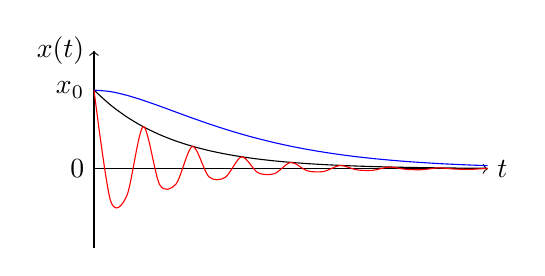
\begin{tikzpicture}
      \draw[->] (0,0) -- (5,0) node[right] {$t$};
      \draw[->] (0,-1) -- (0,1.5) node[left] {$x(t)$};
      \draw[domain=0:5,smooth,variable=\x,black] plot ({\x},{exp(-\x)});
      \draw[domain=0:5,smooth,variable=\x,blue] plot ({\x},{(1+\x)*exp(-\x)});
      \draw[domain=0:5,smooth,variable=\x,red] plot ({\x},{exp(-\x)*cos(10*\x*180/pi)});
      \draw (0,0) node[left]{0};
    \draw (0,1) node[left]{$x_0$};
\end{tikzpicture}
\end{center}
\end{thm}
\begin{proof}
We will state without proof that $e^{\lambda t}$ is an eigenfunction for the differential operator $\frac{d}{dt}$, i.e.
$$\frac{d}{dt}e^{\lambda t}=\lambda e^{\lambda t}$$
Hence, the general eigensolution for this second order linear differential equation will be $e^{\lambda t}$ and hence we will obtain a characteristic equation
$$\lambda^2+\gamma\lambda+\omega_0^2=0$$
which has the solutions
$$\lambda=0.5\bigg(-\gamma\pm\sqrt{\gamma^2-4\omega_0^2}\bigg)$$
The exact form of the solution depends on the discriminant $\gamma^2-4\omega_0^2$, in another words, the relative values of $\gamma$ and $\omega_0$. 
\begin{enumerate}
\item When $\gamma<2\omega_0$, one will yield complex solutions $\lambda=-0.5\gamma\pm i\omega_ut$ where $\omega_u=\sqrt{\omega_0^2-0.25\gamma^2}$ as desired. The general solution will be a linear combination of $e^{-0.5\gamma+i\omega_ut}$ and $e^{-0.5\gamma-i\omega_ut}$. \item When $\gamma>2\omega_0$, one will yield real distinct solutions $\lambda_{1,2}=0.5\gamma\pm\sqrt{0.25\gamma^2-\omega_0^2}$ such that the general solution will be a linear combination of $e^{\lambda_1 t}$ and $e^{\lambda_2t}$. The exact coefficients depends on the initial conditions. 
\item Lastly, when $\gamma=2\omega_0$, one will yield a single real but repeated root. The only solution is $x=e^{-0.5\gamma t}$. To obtain a second linearly independent solution, we will use the Wronskian method to obtain $te^{-0.5\gamma t}$.
\end{enumerate}
\end{proof}
\begin{figure}[H]
\begin{minipage}{\linewidth}
\subfloat[]{\includegraphics[width=.5\linewidth]{damping1.PNG}}
\subfloat[]{\includegraphics[width=0.5\linewidth]{damping2.PNG}}
\end{minipage}
\caption{Plotted on Mathematica: Various damping for $\omega_0=1$ where the damping parameters for critical damping, underdamping and overdamping are $\gamma=2$, $\gamma=0.3$ and $\gamma=2.5$ respectively (a) for the initial conditions $x_0=1$ and $v_0=2$ (b) for the initial conditions $x_0=-1$ and $v_0=2$.}
\end{figure}
\begin{thm}[Underdamped Oscillation]
Suppose $\gamma<2\omega_0$, such that the damping is small, then the oscillation is said to be underdamped. The general solution for an underdamped solution is
$$x(t)=e^{-0.5\gamma t}(c_1\cos(\omega_ut)+c_2\sin(\omega_ut))$$
where $\omega_u=\sqrt{\omega_0^2-0.25\gamma^2}$ and the constants $c_1$ and $c_2$ are dependent on the initial conditions. If the initial conditions are $x(t=0)=x_0$ and $\dot{x}(t=0)=v_0$, then the solution is
$$x(t)=e^{-0.5\gamma t}\bigg(x_0\cos(\omega_ut)+\frac{v_0+0.5\gamma x_0}{\omega_u}\sin(\omega_ut)\bigg)$$
which is an oscillatory solution with a decaying envelope.
\end{thm}
\begin{proof}
The general solution was taken from the previous theorem. The time derivative is
$$\dot{x}(t)=-\frac{\gamma}{2}e^{-0.5\gamma t}(c_1\cos(\omega_ut)+c_2\sin(\omega_ut))+\omega_ue^{-0.5\gamma t}(-c_1\sin(\omega_ut)+c_2\cos(\omega_ut))$$
Hence, the constants are $c_1=x_0$ and $c_2=\frac{v_0+0.5\gamma x_0}{\omega u}$.
\end{proof}
\begin{cor}[Loss of Energy in Underdamped Oscillations]
The mean loss of energy is $-b\langle\dot{x}^2\rangle$.
\end{cor}
\begin{proof}
The mean value for energy is
$$\langle E\rangle=0.5m\langle\dot{x}^2\rangle+0.5k\langle x^2\rangle=0.5m\omega_0^2A^2e^{-\gamma t}$$
and the mean rate of change of energy is thus
$$\frac{d}{dt}\langle E\rangle=-\gamma\langle E\rangle=-b\langle\dot{x}^2\rangle$$
\end{proof}
Note that the larger the friction term, the longer the period but it takes a shorter time and fewer oscillation cycles for the amplitude to decay to zero. Moreover, the amplitude peaks are bounded by $\pm e^{-0.5\gamma t}$ which explains why the rate of decrease of amplitude is higher for a larger friction term. The amplitude thus exponentially decays.

\begin{defi}[Quality Factor]
We define the quality factor, $Q$ as
$$Q\equiv\frac{\omega_0}{\gamma}$$
Quality factor is defined to be the \emph{number of cycles for the amplitude to decrease by a factor of $e^{-\pi}$}. To complete $Q$ number of cycles, the time taken can be obtained from $\omega_ut=2\pi Q$. For very light damping, $\omega_u\approx\omega_0$ and one can approximate this as $\frac{2\pi Q}{\omega_0}=\frac{2\pi}{\gamma}$ such that $e^{-0.5\gamma t}=e^{-0.5\gamma(2\pi/\gamma)}=e^{-\pi}$. Since the condition for light damping is $\gamma<2\omega_0$, $Q>0.5$. The greater the quality factor, the smaller the damping.
\end{defi}
\begin{defi}[Logarithmic Decrement of Amplitude]
Now, let's consider the ratio of amplitude of the $(n+1)$th peak to that of the $n$th peak, bearing in mind that the amplitudes are related by the exponential term $e^{-0.5\gamma t}$:
$$\frac{a_{n+1}}{a_n}=e^{-\gamma(t_{n+1}-t_n)}$$
The time difference between the $n$th peak and the $(n+1)$th peak is related to the period of the under-damped oscillation which is $\frac{2\pi}{\omega_u}$.\\[5pt]
We denote the quantity $\Delta$ to be the logarithmic decrement $\ln(a_{n+1}/a_n)$:
$$\Delta=\ln(e^{-\frac{1}{2}\frac{2\pi\gamma}{\omega_u}})=-\frac{\pi\gamma}{\omega_u}\approx-\frac{\pi\gamma}{\omega_0}=-\frac{\pi}{Q}$$
The number of cycles for the amplitude to fall by a factor $e$ is thus
$$\bigg|\frac{1}{\Delta}\bigg|=\frac{Q}{\pi}$$
The quality factor can thus also be defined as the number of radians of oscillations for the amplitude to fall by a factor of $e$.
\end{defi}
\begin{thm}[Overdamped Oscillation]
If $\gamma>2\omega_0$, where there is a large friction, then the system is said to be overdamped such that no oscillation occurs and the displacement goes asymptotically to zero. The general solution is
$$x(t)=c_+e^{-\mu_+t}+c_-e^{-\mu_-t}$$
where $\mu_{\pm}=\frac{1}{2}\gamma\pm\sqrt{0.25\gamma^2-\omega_0^2}$ such that $\mu_+>0.5\gamma>\omega_0$ and that $c_{\pm}$ are constants dependent on initial conditions. With the initial conditions $x(t=0)=x_0$ and $\dot{x}(t=0)=v_0$, the constants are
$$c_+=\frac{x_0\mu_-+v_0}{\mu_--\mu_+},\quad c_-=\frac{x_0\mu_++v_0}{\mu_+-\mu_-}$$
\end{thm}
\begin{proof}
Easy to verify.
\end{proof}
Observe that for overdamping, the quality factor $Q<0.5$.
\begin{cor}
For heavy damping, the greater the friction, the amplitude decreases at a slower rate and it takes a much longer time for the amplitude to reach zero. In fact, for certain initial conditions, there exists a time where the amplitude is zero (other than when $t\rightarrow\infty$).
\end{cor}
\begin{proof}
One may compute this time where $x=0$:
$$c_+e^{-\mu_+t}+c_-e^{-\mu_-t}=0\implies t=\frac{1}{\mu_+-\mu_-}\ln\bigg(-\frac{c_+}{c_-}\bigg)$$
Notice that if $\mu_+>\mu_-$, $e^{-\mu_+t}$ will decrease at a faster rate. This is particularly dominant when its coefficient is larger than $e^{-\mu_-t}$.
\end{proof}
\begin{thm}[Very Heavy Damping]
For very heavy damping, where $\gamma>>\omega_0$, $x(t)\approx Ce^{-\omega_0^2t/\gamma}$.
\end{thm}
\begin{proof}
For very heavy damping, we have $\gamma>>\omega_0$ and hence
$$\mu_\pm=\frac{\gamma}{2}\bigg(1\pm\bigg(1-\frac{4\omega_0^2}{\gamma^2}\bigg)^{0.5}\bigg)$$
which is approximately $\mu_+\approx\gamma$ or $\mu_-\approx\frac{\omega_0^2}{\gamma}$ (which is very small). Since the term $e^{-\mu_+t}$ reaches zero much faster, we can approximate
$$x(t)=c_+e^{-\mu_+t}+c_-e^{-\mu_-t}\approx c_-e^{-\omega_0^2t/\gamma}$$
Essentially, the slower decaying exponential dominates.
\end{proof}
\begin{defi}[Relaxation Time for Very Heavy Damping]
One defines the relaxation time for very heavy damping, $\tau_r=\frac{1}{\mu_2}=\frac{\gamma}{\omega_0^2}$, which is the time taken for $x(t)$ to be a factor $e^{-1}$ of the initial value.
\end{defi}
\begin{thm}[Critically Damped Oscillation]
Critical damping occurs when $\gamma=2\omega_0$ and subjected to the initial conditions $x(0)=x_0$ and $v(0)=v_0$, we have
$$x(t)=(x_0+(v_0+0.5\gamma x_0)t)e^{-0.5\gamma t}$$
\end{thm}
\begin{proof}
Using the general solution for $\gamma=2\omega_0$ and differentiate it:
$$\dot{x}=c_2e^{-0.5\gamma t}-0.5\gamma(c_1+c_2t)e^{-0.5\gamma t}$$
Then after using the initial conditions, we get our desired result. 
\end{proof}
Observe that the quality factor is $Q=0.5$.
\begin{cor}
Critically damping gives the fastest return to the equilibrium position (but still asymptotically reaches zero), without undergoing oscillation.
\end{cor}
\begin{eg}
If a current meter is critically damped, the instrument is good at measuring alternating current with angular frequency $\omega$ if the relaxation time (time taken for amplitude to be a factor of $e^{-1}$ of its initial value) is a lot less
than a period of the oscillation to be measured:
$$\frac{2/\gamma}{2\pi/\omega}=\frac{\omega}{\gamma\pi}<<1$$
\end{eg}
\begin{cor}
For critically damped and heavy damping systems, the displacement will only be zero for at most once. It is also possible that for some initial conditions, the displacement is never zero despite asymptotically reaching zero.
\end{cor}
\begin{proof}
We first consider the critically damped system. For $x(t=\tau)=0$, we require $(x_0+(v_0+0.5\gamma x_0)\tau)=0$ and this only has at most one solution.
$$\tau=\frac{-x_0}{v_0+0.5\gamma x_0}$$
Clearly, for some values of $x_0$ and $v_0$, $\tau<0$ and in that case, the system will never be at zero. As for overdamped systems, we have already find
$$\tau=\frac{1}{\mu_+-\mu_-}\ln\bigg(-\frac{c_+}{c_-}\bigg)=\frac{1}{2\sqrt{0.25\gamma^2-\omega_0^2}}\ln\bigg(\frac{x_0\mu_-+v_0}{x_0\mu_++v_0}\bigg)$$
where $\mu_\pm$ as defined. We can't simplify this expression any further. Likewise, when $\tau<0$, then the system will never be at zero.
\end{proof}
\begin{defi}[Second Order Driven Oscillation]
We will now consider the presence of a sinusoidal driving force in a damped oscillatory system such that the equation of motion has the form
$$\ddot{x}+\gamma\dot{x}+\omega_0^2x=f_0e^{i\omega t}$$
Notice that the driving frequency, $\omega$, is not necessarily equal to the natural frequency of oscillation, $\omega_0$.
\end{defi}
\begin{thm}[General Solution for Forced Damped Oscillations]
The general solution for a forced damped oscillatory system is a linear combination of the general solution for an unforced damped oscillatory system (associated homogeneous differential equation) and the particular solution for the forced function.
\end{thm}
\begin{proof}
Since this is a linear differential equation, the general solution must be a linear combination of the complementary solution of the associated homogeneous equation and the particular solution. This is a consequence of superposition and linearity.
\end{proof}
\begin{thm}[Transient Solution]
The transient solution, complementary solution of the forced damped oscillation, is just the general solution of the corresponding homogeneous second order differential equation.
\end{thm}
\begin{proof}
Suppose $y$ and $y_p$ are distinct solutions to the non-homogeneous differential equation, then $y-y_p$ is the solution to the corresponding homogeneous solution.
\end{proof}
\begin{thm}[Steady State Solution]
The steady state solution, particular solution of the forced damped oscillation, has the form $x(t)=Ae^{i(\omega t+\phi)}$ such that the response amplitude and phase respectively are
$$|A(\omega)|=\frac{f_0}{\sqrt{(\omega_0^2-\omega^2)^2+\gamma^2\omega^2}},\quad\phi=\tan^{-1}\bigg(\frac{-\gamma\omega}{\omega_0^2-\omega^2}\bigg)$$
Then the steady state solution will be
\begin{eqnarray}
x(t)&=&\frac{f_0}{\sqrt{(\omega_0^2-\omega^2)^2+\gamma^2\omega^2}}\cos\bigg(\omega t+\tan^{-1}\bigg(\frac{-\omega\gamma}{\omega_0^2-\omega^2}\bigg)\bigg)\nonumber\\&=&\frac{(\omega_0^2-\omega^2)f_0}{(\omega_0^2-\omega^2)^2+\gamma^2\omega^2}\cos(\omega t)+\frac{\gamma\omega f_0}{(\omega_0^2-\omega^2)^2+\gamma^2\omega^2}\sin(\omega t)\nonumber
\end{eqnarray}
\end{thm}
\begin{proof}
Substitute the suggested solution form to the equation of motion, we get
$$f_0=A(-\omega^2+i\gamma\omega+\omega_0^2)e^{i\phi}$$
After manipulation, and taking the modulus of the amplitude, we get our desired result. On the other hand, the phase can be determined using:
$$\tan(\phi)=\frac{e^{i\phi}-e^{-i\phi}}{e^{i\phi}+e^{-i\phi}}=\frac{-\gamma\omega}{\omega_0^2-\omega^2}$$
Alternatively, we may use the phasor method, noting that $\gamma\omega A$ has a phase difference of $\pi/2$ with respect to $\omega_0^2A$. However, $\omega^2A$ is in phase with $\omega_0^2A$. Since $\gamma\omega>0$, on the Argand Diagram, $0\leq-\phi\leq\pi$ such that $-\pi\leq\phi\leq 0$.
\end{proof}
Below are plots of the response amplitude and phase for light (black), critical (blue) and heavy (red) damping respectively. Note for the phase, there are two branches and they are made continuous by taking the second branch and deduct $\pi$ radians.
\begin{center}
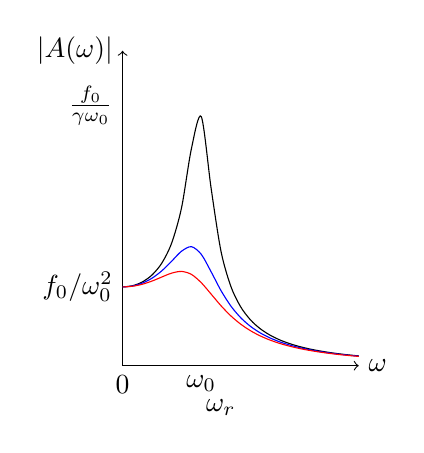
\begin{tikzpicture}
      \draw[->] (0,0) -- (3,0) node[right] {$\omega$};
      \draw[->] (0,0) -- (0,4) node[left] {$|A(\omega)|$};
      \draw[domain=0:3,smooth,variable=\x,black] plot ({\x},{1/sqrt((1-\x^2)^2+0.1*\x^2)});
      \draw[domain=0:3,smooth,variable=\x,blue] plot ({\x},{1/sqrt((1-\x^2)^2+0.5*\x^2)});
      \draw[domain=0:3,smooth,variable=\x,red] plot ({\x},{1/sqrt((1-\x^2)^2+0.9*\x^2)});
      \draw (0,0) node[below]{0};
\draw (0,1) node[left]{$f_0/\omega_0^2$};
\draw (1,0) node[below]{$\omega_0$};
\draw (1.25,-0.3) node[below]{$\omega_r$};
\draw (0,3.3) node[left]{$\frac{f_0}{\gamma\omega_0}$};
\end{tikzpicture}
\hspace{3cm}
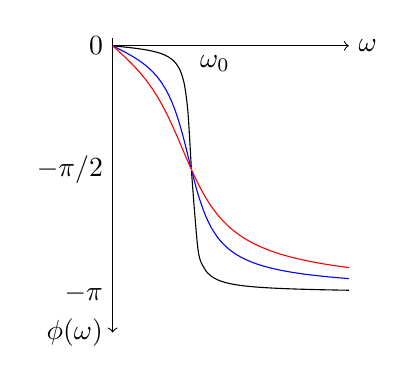
\begin{tikzpicture}
      \draw[->] (0,0) -- (3,0) node[right] {$\omega$};
      \draw[->] (0,0.1) -- (0,-pi-0.5)  node[left] {$\phi(\omega)$};
      \draw[domain=0:0.999,smooth,variable=\x,black] plot ({\x},{rad(atan(-0.1*\x/(1-\x^2)))});
      \draw[domain=1.001:3,smooth,variable=\x,black] plot ({\x},{rad(atan(-0.1*\x/(1-\x^2)))-pi});
      \draw[domain=0:0.999,smooth,variable=\x,blue] plot ({\x},{rad(atan(-0.5*\x/(1-\x^2)))});
      \draw[domain=1.001:3,smooth,variable=\x,blue] plot ({\x},{rad(atan(-0.5*\x/(1-\x^2)))-pi});
      \draw[domain=0:0.999,smooth,variable=\x,red] plot ({\x},{rad(atan(-0.9*\x/(1-\x^2)))});
      \draw[domain=1.001:3,smooth,variable=\x,red] plot ({\x},{rad(atan(-0.9*\x/(1-\x^2)))-pi});
      \draw (0,0) node[left]{0};
      \draw (0,-pi/2) node[left]{$-\pi/2$};
      \draw (0,-pi) node[left]{$-\pi$};
    \draw (1.3,0) node[below]{$\omega_0$};
\end{tikzpicture}
\end{center}
\newpage
\begin{cor}
The phase of the damped forced oscillation at various regimes are as follow:
\begin{itemize}
\item At low driving frequencies, $\omega\approx0$, the system oscillates in phase with the driving force, $\phi=0$. 
\item When the system is at resonance, $\omega=\omega_0$ the system lags behind the driving force by a phase $\pi/2$. 
\item At high driving frequencies, $\omega\approx\infty$, the phase lag becomes $\pi$. 
\item The larger the damping, $\gamma\rightarrow\infty$, the phase shifts from 0 to $-\pi$ less sharply.
\end{itemize}
\end{cor}
\begin{cor}
The amplitude profile as a function of $\omega$, starts at $\omega=0$ with an amplitude of $\frac{f_0}{\omega_0^2}$ and for large amplitudes, it approximately has the form $\frac{f_0}{\omega^2}$.
\end{cor}
\begin{proof}
$\lim_{\omega\rightarrow0}|A(\omega)|=\frac{f_0}{\omega_0^2}$ and $\lim_{\omega\rightarrow+\infty}|A(\omega)|=\lim_{\omega\rightarrow\infty}\frac{f_0}{\omega^2}=0$
\end{proof}
\begin{cor}
If the steady state term is represented by a vector of constant length rotating anticlockwise at the angular velocity $\omega$ of the driving force, then its tip traces a circle. Upon this is superposed the transient term vector which traces a spiral and rotates with angular velocity $\sqrt{\omega_0^2-\gamma^2/4}$.
\end{cor}
\begin{proof}
The transient vector's length decays exponentially and as the vector traverses $2\pi$ radians, its tip traces a spiral.
\end{proof}
\begin{cor}[Displacement, Velocity and Acceleration Response]
Given an external forcing $F_0e^{i\omega t}$, the displacement, velocity and acceleration response respectively are:
$$x(t)=\frac{f_0}{(\omega_0^2-\omega^2)^2+\omega^2\gamma^2}[\cos(\omega t)(\omega_0^2-\omega^2)+\sin(\omega t)\omega \gamma]$$
$$v(t)=\frac{f_0\omega}{(\omega_0^2-\omega^2)^2+\omega^2\gamma^2}[-\sin(\omega t)(\omega_0^2-\omega^2)+\cos(\omega t)\omega \gamma]$$
$$a(t)=\frac{-\omega^2f_0}{(\omega_0^2-\omega^2)^2+\omega^2\gamma^2}[\cos(\omega t)(\omega_0^2-\omega^2)+\sin(\omega t)\omega\gamma]$$
\end{cor}
\begin{proof}
The expressions are obtained by simplifying $x(t)=\text{Re}[\frac{F_0e^{i\omega t}}{i\omega b+(k-m\omega^2)}]$, $v(t)=\text{Re}[\frac{i\omega F_0e^{i\omega t}}{i\omega b+(k-m\omega^2)}]$ and $a(t)=\text{Re}[\frac{-\omega^2 F_0e^{i\omega t}}{i\omega b+(k-m\omega^2)}]$ where $\gamma=b/m$ and $\omega_0^2=k/m$. Interesting limits are $\lim_{\omega\rightarrow0}x(t)=\frac{f_0}{\omega_0^2}$ and $\lim_{\omega\rightarrow\infty}a(t)=f_0$.
\end{proof}
The plots for the amplitudes of each give
\begin{center}
\begin{tikzpicture}
      \draw[->] (0,0) -- (4,0) node[right] {$\omega$};
      \draw[->] (0,-1) -- (0,1.5) node[left] {$x(\omega)$};
      \draw[domain=0:4,smooth,variable=\x,black] plot ({\x},{1/sqrt((1-\x^2)^2+\x^2});
      \draw (0,0) node[left]{0};
      \draw (0,1) node[left]{$f_0/k\omega_0^2$};
      \draw (1,0) node[below]{$\omega_{res}$};
\end{tikzpicture}
\hspace{0.01cm}
\begin{tikzpicture}
      \draw[->] (0,0) -- (6,0) node[right] {$\omega$};
      \draw[->] (0,-1) -- (0,1.5) node[left] {$v(\omega)$};
      \draw[domain=0.01:6,smooth,variable=\x,black] plot ({\x},{1/sqrt((1-\x^2)^2/\x^2+1});
      \draw (0,0) node[left]{0};
      \draw (1,0) node[below]{$\omega_0$};
\end{tikzpicture}
\hspace{0.01cm}
\begin{tikzpicture}
      \draw[->] (0,0) -- (4,0) node[right] {$\omega$};
      \draw[->] (0,-1) -- (0,1.5) node[left] {$a(\omega)$};
      \draw[domain=0:4,smooth,variable=\x,black] plot ({\x},{\x^2/sqrt((1-\x^2)^2+\x^2});
      \draw (0,0) node[left]{0};
      \draw (0,1) node[left]{$f_0$};
      \draw (1.3,0) node[below]{$\omega_{res}$};
\end{tikzpicture}
\end{center}
\begin{Note}
In a similar analogy to the electron in an atom irradiated by light, the $\sin(\omega t)$ component of the displacement response represents the characteristic absorption coefficient (lags driving force by $\frac{\pi}{2}$ and is at maximum at $\omega_0$) while the $\cos(\omega t)$ component represents the energy storing fraction (in anti-phase with respect to the driving force, which in turn governs the refractive index). 
\end{Note}
\begin{thm}[Resonance]
The resonance for displacement occurs at the resonant frequency 
$$\omega_r=\omega_0\sqrt{1-\frac{\gamma^2}{2\omega_0^2}}$$ 
with a maximal amplitude of $\frac{f_0}{\gamma\omega_0}$.
\end{thm}
\begin{proof}
To find the resonant frequency, one needs to maximize $|A(\omega)|$. This is most easily done by minimizing the square of this quantity with respect to $\omega^2$:
$$\frac{\partial}{\partial(\omega^2)}[(\omega_0^2-\omega^2)^2+\gamma^2\omega^2]^{-1/2}=0\implies\omega_r=\omega_0\sqrt{1-1/(2Q^2)}$$
where $Q=\frac{\omega_0}{\gamma}$. 
In particular, if damping is small $(\gamma<<\omega_0)$, then the resonance frequency is approximately equal to the natural frequency, i.e. $$\lim_{\gamma\rightarrow0}\omega_r=\omega_0$$
At this resonant frequency, the amplitude is $\lim_{\omega\rightarrow\omega_r}|A(\omega)|=\frac{f_0}{\sqrt{0.25\gamma^4+\gamma^2(\omega_0^2-0.25\gamma^2)}}=\frac{f_0}{\gamma\omega_0}$ and this approaches infinity as $\gamma$ approaches zero, i.e. negligible damping.
\end{proof}
Hence, systems with lower damping have a peak amplitude much closer to the resonance frequency. As damping increases, the peak amplitude is shifted to the left and the peak amplitude is much smaller than before.
\begin{cor}
Velocity resonance occurs when $\omega=\omega_0$, independent of the damping. At this frequency, the velocity is exactly in phase with the driving force.
\end{cor}
\begin{proof}
We have
$$v_0=\frac{f_0}{\sqrt{(\omega_0^2-\omega^2)^2/\omega^2+\gamma^2}}$$
which clearly has a maximum at $\omega_0$. We have $\arg(v_0/f_0)=\tan^{-1}(\frac{\omega_0^2-\omega^2}{\gamma\omega})$, which is in phase when $\omega=\omega_0$.
\end{proof}
\begin{cor}
Acceleration resonance occurs when $\omega=\omega_0(1-\frac{1}{2Q^2})^{-0.5}$.
\end{cor}
\begin{proof}
Acceleration is $a=-\frac{f}{(\omega_0^2-\omega^2)/\omega^2+(i\gamma/\omega)}$, which occurs at $\omega_0(1-(2Q^2)^{-1})^{-0.5}$.
\end{proof}
\begin{thm}[Power of Forced Oscillator]
The power of a forced oscillator is $P=\text{Re}[F]\text{Re}[v]$, where $F$ and $v$ are complex quantities. The time-averaged power is then
$$\langle P\rangle=\frac{1}{2}\text{Re}[F_0v_0^*]$$
\end{thm}
\begin{proof}
The product of two complex quantities will be
$$\text{Re}[A]\text{Re}[B]=\frac{1}{2}(A+A^*)\frac{1}{2}(B+B^*)=\frac{1}{4}(AB+A^*B^*+AB^*+A^*B)=\frac{1}{2}\text{Re}[AB+AB^*]$$
Hence,
$$P=\frac{1}{2}\text{Re}[F_0v_0e^{2i\omega t}+F_0v_0^*]\implies\langle P\rangle=\frac{1}{2}\text{Re}[F_0v_0^*]=\frac{1}{2}F_0v_0\cos(\phi_F-\phi_v)$$
where $\phi_F=\phi_v$ if both the force and velocity are in phase such that the $\langle P\rangle=\frac{1}{2}F_0v_0$. Similarly, if they are $\frac{\pi}{2}$ out of phase, then $\langle P\rangle=0$.
\end{proof}
\begin{cor}
For our forced oscillator, the time-averaged power is
$$\langle P(\omega)\rangle=\frac{m\gamma\omega^2f_0^2}{2((\omega_0^2-\omega^2)^2+\gamma^2\omega^2)}$$
\end{cor}
\begin{proof}
The time-averaged power is
$$\frac{1}{2}\text{Re}[F\dot{x}^*]=\frac{1}{2}\text{Re}[i\omega mf_0Ae^{-i\phi}]=\frac{1}{2}A\omega m f_0\sin\phi=\frac{m}{2}\frac{\omega f_0^2}{\sqrt{(\omega_0^2-\omega^2)^2+\gamma^2\omega^2}}\frac{\omega\gamma}{\sqrt{(\omega_0^2-\omega^2)^2+\gamma^2\omega^2}}$$
where the phase difference between the driving force and velocity response $\phi$ satisfies $\tan\phi=-\frac{\gamma\omega}{\omega_0^2-\omega^2}$.
\end{proof}
\begin{cor}[Power Supplied by Driving Force]
By conservation of energy, the time-averaged power supplied by the driving force is equal to the negative of the time-averaged power dissipated by the damping force.
\end{cor}
\begin{proof}
The time-averaged power supplied by the driving force is
$$\langle P_{\text{driving}}\rangle=\frac{1}{2}\text{Re}[F_0v_0^*]=\frac{1}{2}\text{Re}\bigg[v_0m\bigg(\frac{(\omega_0^2-\omega^2)}{i\omega}+\gamma\bigg)v_0^*\bigg]=\frac{1}{2}\gamma m|v_0|^2=-\frac{1}{2}\gamma m|v_0|(-|v_0|)$$
which is equal to $-\langle P_{dissipated}\rangle$, consistent with the previous result. The power supplied by this driving force is maximum during resonance.
\end{proof}
\begin{center}
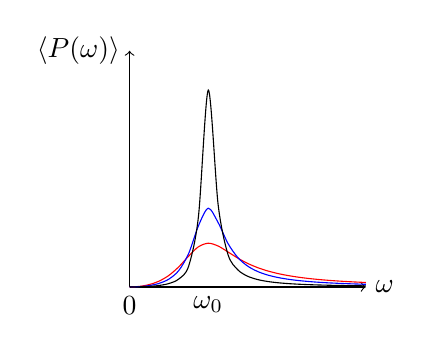
\begin{tikzpicture}
      \draw[->] (0,0) -- (3,0) node[right] {$\omega$};
      \draw[->] (0,0) -- (0,3) node[left] {$\langle P(\omega)\rangle$};
      \draw[domain=0:3,smooth,variable=\x,red] plot ({\x},{(0.9*\x^2)/(2*((1-\x^2)^2+(0.9*\x)^2))});
     \draw[domain=0:3,smooth,variable=\x,blue] plot ({\x},{(0.5*\x^2)/(2*((1-\x^2)^2+(0.5*\x)^2))});
     \draw[domain=0:3,smooth,variable=\x,black] plot ({\x},{(0.2*\x^2)/(2*((1-\x^2)^2+(0.2*\x)^2))});
     \draw (1,0) node[below]{$\omega_0$};
      \draw (0,0) node[below]{0};
\end{tikzpicture}
\end{center}
\begin{thm}[Power Addition]
A driving force $F(t) =F_1(t) +F_2(t)$ is applied to a damped oscillator, where $F_j(t) =Re[F_je^{i\omega_jt}]$ for $j=1,2$. Show that, if $\omega_1\neq\omega_2$,the mean power absorbed by the system is given by $\langle P\rangle=\langle P_1\rangle+\langle P_2\rangle$ where $\langle P_i\rangle$ is the mean powers absorbed if only $F_i$ were applied. But if $\omega_1=\omega_2$, $\langle P\rangle =\langle P_1\rangle+\langle P_2\rangle+\frac{F_1F_2}{Z_m}\cos\phi$ where $\phi$ is the phase difference between the driving force and the velocity response.
\end{thm}
\begin{proof}
Since we are applying to the same damped oscillator with mechanical impedance $Z_m$, 
$$P_i=F_i\cos(\omega_it)\frac{F_i}{Z_m}\cos(\omega_it-\phi)\implies\langle P_i\rangle=\frac{F_i^2}{Z_mT}\int_0^T\cos^2(\omega_1t)\cos\phi+\cos(\omega_1t)\sin(\omega_1t)\sin\phi dt=\frac{F_i^2}{2Z_m}\cos\phi$$
where $i=1,2$. But for $F=F_1+F_2$, the corresponding power is
$$P=(F_1\cos(\omega_1t)+F_2\cos(\omega_2t))\bigg(\frac{F_1}{Z_m}\cos(\omega_1t-\phi)+\frac{F_2}{Z_m}\cos(\omega_2t-\phi)\bigg)$$
Taking the time-averaged, we have $\langle P\rangle=\langle P_1\rangle+\langle P_2\rangle$ for $\omega_1\neq\omega_2$ since the time-averaged cross terms of different frequencies vanish. But for $\omega_1=\omega_2$, we have $\langle P\rangle=\langle P_1\rangle+\langle P_2\rangle+\frac{F_1F_2}{Z_m}\cos\phi$. Suppose the system achieve resonance at $\omega_0$, and the driving forces are of different frequencies $\omega_j$, then there will be resonance peaks at $\omega_j=\omega_0$ and of amplitude $\frac{F_j^2}{2Z_m}$.
\end{proof}
\begin{Note}[Linear System driven at multiple frequencies]
Consider driving a system with sum of two harmonic forces: 
$$F(t)=F_1\cos(\omega_1t+\alpha_1)+F_2\cos(\omega_2t+\alpha_2)$$
Suppose the driving forces have the same angular frequency $\omega_1=\omega_2=\omega$, then the resultant amplitude will be $A^2=A_1^2+A_2^2+2A_1A_2\cos(\alpha_2-\alpha_1)$. If we choose equal driving forces, $F_1=F_2$, then $A^2=2A_1^2(1+\cos(\alpha_2-\alpha_1))$. In-phase driving: double the amplitude response and quadruple the power. Anti-phase driving: no response.\\[5pt]
However, in practice, unless the driving terms $F_1$ and $F_2$ are highly stable, the term $\cos(\alpha_2-\alpha_1)$ is likely to drift and average to zero over time. The driven response will be the quadrature sum of the individual responses, i.e. incoherent forces. Hence, we add the energies not the amplitudes.
\end{Note}
\begin{thm}[Full Width Half Maxima of Resonance]
The width of the resonance peak for the displacement, defined at half the maximum power is equal to $\gamma$.
\end{thm}
\begin{proof}
Since the full-width half maxima is the width of the power curve (related to $|\dot{x}|^2$) at half the maximum power, then
$$\frac{\gamma^2\omega^2}{(\omega_0^2-\omega^2)^2+\gamma^2\omega^2}=\frac{1}{2}\implies(\omega_0^2-\omega^2)^2=\gamma^2\omega^2\implies\omega_0^2-\omega^2=\pm\gamma\omega\implies\Delta\omega=\gamma$$
This is the width of the peak, which increases when damping increases. This explains why near resonance, the peak appears large in amplitude and narrow in width. The quality factor for driven systems, can thus be defined as $\frac{\omega_0}{\Delta\omega}$.
\end{proof}
\begin{center}
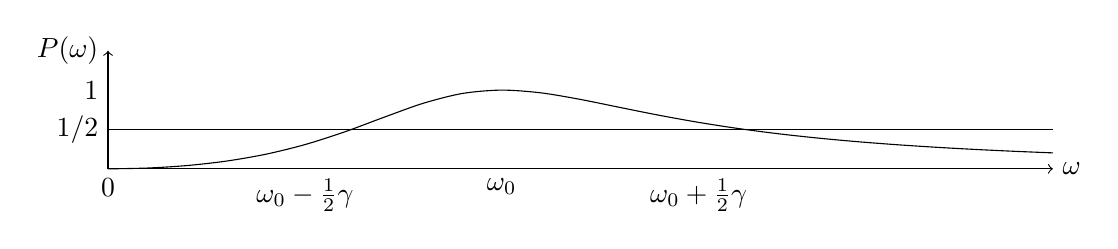
\begin{tikzpicture}
      \draw[->] (0,0) -- (12,0) node[right] {$\omega$};
      \draw[->] (0,0) -- (0,1.5) node[left] {$P(\omega)$};
      \draw[domain=0:12,smooth,variable=\x,black] plot ({\x},{(0.2*\x)^2/((1-(0.2*\x)^2)^2+(0.2*\x)^2)});
      \draw[domain=0:12,smooth,variable=\x,black] plot ({\x},{0.5});
      \draw (0,0) node[below]{0};
      %\draw 
%\foreach \x in {1,2,...,4} {%
    %\draw ($(\x,0) + (0,-\TickSize)$) -- ($(\x,0) + (0,\TickSize)$);
%}

\draw (0,1) node[left]{1};
\draw (0,1/2) node[left]{1/2};
\draw (2.5,0) node[below]{$\omega_0-\frac{1}{2}\gamma$};
\draw (5,0) node[below]{$\omega_0$};
\draw (7.5,0) node[below]{$\omega_0+\frac{1}{2}\gamma$};
\end{tikzpicture}
\end{center}
\subsubsection*{Miscellaneous}
\begin{Note}[Driven Electrical Circuit - LCR]
Let's consider the electrical equivalent of driven damped oscillation
$$\ddot{q}+\gamma\dot{q}+\omega_0^2q=\frac{V}{L}$$
where $\gamma=\frac{R}{L}$, $Q=\frac{\omega_0}{\gamma}=\frac{1}{R}\sqrt{L/C}$ and $\omega_0=\frac{1}{\sqrt{LC}}$. $V_L$, $V_C$ and $V_R$ (and $I$) peaks above $\omega_0$, below $\omega_0$ and at resonant frequency $\omega_0$ respectively. This is equivalent to acceleration, displacement and velocity respectively in the mechanical analog. Since $Z=\frac{V_0}{I_0}$, we have $\langle P\rangle=\frac{1}{2}\text{Re}[V_0I_0^*]=\frac{1}{2}|V_0|^2\text{Re}[1/Z]=\frac{1}{2}|I_0|^2\text{Re}[Z]=\frac{1}{2}I_0^2R$. Comparing with the mechanical equivalent, $\langle P\rangle=\frac{1}{2}|v_0|^2\text{Re}[Z]$.
\end{Note}
\begin{Note}[Atomic Oscillators]
Consider a semi-classical model of a Hydrogen atom: a uniform spherical cloud of radius $a$, driven by an electric field $E_0e^{i\omega t}$. If the proton moves a distance $x$ from the centre of the electron cloud, it has a Hooke-law restoring force with effective spring constant $\frac{e^2}{4\pi\epsilon_0a^3}$. The undamped oscillation frequency will be about $10^{16}$ Hz for $a=50$ pm. Optical light has $f_{blue}\approx8\times10^{14}$ Hz, suggesting atoms should behave as oscillators driven below resonance when illuminated by light. The origin of damping is the Larmor radiation (as the charge oscillates, it radiates energy) of average rate $\frac{e^2x_0^2\omega^4}{12\pi\epsilon_0c^3}$. The mean energy of the electron oscillating is $W=\frac{1}{2}m_e\omega^2x_0^2$ and so the rate of decay is $-P_{rad}=-\frac{e^2\omega^2}{6\pi\epsilon_0c^3m_e}W$, i.e. the energy decays exponentially. But a lightly damped oscillator's energy decays with time constant $1/\gamma$ where $\gamma\approx1.3\times10^{10}$s$^{-1}$ with $Q=\omega_0/\gamma\approx10^6$.
\end{Note}
\begin{Note}[Anharmonic Oscillations]
Consider a symmetric, anharmonic potential $V(x)=0.5kx^2(1+0.5\alpha x^2)$ such that the equation of motion is $\ddot{x}+(1+\alpha x^2)\omega_0^2x=0$. If $\alpha>0$, the potential is hard, i.e. the spring stiffens with extension. On the other hand, if $\alpha<0$, it is soft. We look for solutions when $|\alpha|<<1$, and assume that the mass is at rest at $t=0$, then a suitable solution is
$$x(t)=A(\cos\omega_ft+\epsilon\cos(3\omega_ft)+...)$$
Two unknowns, for small $|\alpha|$, expect $\omega_f\approx\omega_0$ and $\epsilon$ to be small compared to unity. The anharmonic correction is small if $|\alpha A^2|<<1$. Substitute back to the equation of motion, and working to first order in $\alpha A^2$ and $\epsilon$, we have $\omega_f\approx\omega_0(1+(3/8)\alpha A^2)$ and $\epsilon\approx\frac{1}{32}\alpha A^2$. The period is now amplitude-dependent. When we drive a non-linear oscillator with a sinusoidal forcing term, the system will exhibit deterministic chaos and butterfly effect (sensitive to initial conditions). The final driven solution can contain sub-harmonics of the driving period.
\end{Note}

\newpage
\subsection{Waves}
\subsubsection*{Wave equation and energy}
\begin{thm}[Wave Equation]
In general, linear waves can be described by the wave equation
$$\frac{\partial^2}{\partial t^2}\psi(\mathbf{r},t)=v^2\boldsymbol{\nabla^2}\psi(\mathbf{r},t)$$
where the wave solution $\psi$ is a function of space and time.
\end{thm}
We will only prove the one-dimensional wave equation.
\begin{proof}
Consider a string of linear mass density $\lambda$, oscillating in the transverse direction. $\psi(x,t)$ represents the transverse displacement of the string. Consider a small segment of string of length $\delta s$ and mass $\lambda\delta s$, extending horizontally from $x$ to $x+\delta x$. The string accelerates vertically and by Newton's Second Law, and up to a first order approximation:
\begin{eqnarray}
\lambda\delta s\frac{\delta^2\psi}{\delta t^2}&=&T[\sin(\theta(x+\delta x))-\sin(\theta(x))]\nonumber\\\lambda\sqrt{1+\bigg(\frac{\delta \psi}{\delta x}\bigg)^2}\delta x\frac{\delta^2\psi}{\delta t^2}&=&T[\theta(x+\delta x)-\theta(x)]\nonumber\\\lim_{\delta x,\delta\psi,\delta t\rightarrow 0}\lambda\frac{\delta^2\psi}{\delta t^2}&=&T\lim_{\delta x\rightarrow0}\frac{\theta(x+\delta x)-\theta(x)}{\delta x}\nonumber\\\lambda\frac{\partial^2\psi}{\partial t^2}&=&T\frac{\partial\theta}{\partial x}=T\frac{\partial^2\psi}{\partial x^2}\nonumber
\end{eqnarray}
where $\delta x\rightarrow0$, $\delta \psi\rightarrow 0$, leads to $\theta=\frac{\partial\psi}{\partial x}$.
\end{proof}
\begin{defi}[Wave Velocity versus Particle Velocity]
The wave is a pattern that moves with velocity $c$ and amplitude $\psi = \psi(x−ct)$
whereas the individual particles execute periodic motion about a fixed
point with speed $\frac{\partial\psi}{\partial t}$.
\end{defi}
\begin{defi}[Plane Wave]
A plane wave has the planar wavefronts satisfying the geometrical constraint
$$\mathbf{k}\cdot\mathbf{r}=\frac{2\pi}{\lambda}m\lambda=2\pi m$$
where $m\in\mathbb{Z}^+$ is a constant. The exact multiple depends on where the position $\mathbf{r}$ is at from the origin (point of reference). A travelling wave of wavevector $\mathbf{k}$ and angular frequency $\omega$ may be represented by an exponential form
$$\psi(\mathbf{r},t)=e^{i(\mathbf{k}\cdot\mathbf{r}-\omega t)}$$
where the velocity of the wave is $v$ and that $\omega=v|\mathbf{k}|$, and $|\mathbf{k}|^2=k_x^2+k_y^2+k_z^2$
\end{defi}
\begin{defi}[Spherical and Cylindrical Waves]
Suppose a point source produces a wave with spherical symmetry, this wave is a spherical wave. If the source is a line source instead, and the wave has cylindrical symmetry, then the wave is a cylindrical wave.
\end{defi}
\begin{thm}
Spherical waves have the exact form $\psi(r,t)=\frac{f(r\pm vt)}{r}$ while cylindrical waves have the approximate form $\psi(r,t)=\frac{f(r\pm vt)}{\sqrt{r}}$, which is valid as long as $|\frac{f}{4f''r^2}|<<1$. In addition, if $f"'=-k^2f$, then $kr>>1$.
\end{thm}
\begin{proof}
Under spherical symmetry, the wave equation becomes $$v^2\nabla^2\psi(r,t)=v^2\frac{1}{r^2}\frac{\partial}{\partial r}\bigg(r^2\frac{\partial\psi}{\partial r}\bigg)=\frac{\partial^2\psi}{\partial t^2}$$
where $\psi(r,t)$ is independent of $\theta$ and $\phi$. One can verify that $\psi(r,t)=\frac{f(r\pm vt)}{r}$ is a solution, and hence known as a spherical wave. We let $\eta=r\pm vt$, then let $f'$ be $\frac{\partial f(\eta)}{\partial\eta}$. We have
$$\frac{v^2}{r^2}\frac{\partial}{\partial r}\bigg(r^2\frac{\partial\psi}{\partial r}\bigg)-\frac{\partial^2\psi}{\partial t^2}=\frac{v^2}{r^2}\frac{\partial}{\partial r}\bigg(r^2\frac{f'}{r}-\frac{fr^2}{r^2}\bigg)-\frac{\partial}{\partial t}\bigg(\frac{f'}{r}\frac{\partial\eta}{\partial t}\bigg)=\frac{v^2}{r^2}(f'+rf''-f')-\frac{f''}{r}\bigg(\frac{\partial\eta}{\partial t}\bigg)^2=0$$
where $\frac{\partial\eta}{\partial t}=\pm v$ and $\frac{\partial\eta}{\partial r}=1$. Next, under cylindrical symmetry, the wave equation becomes $$v^2\nabla^2\psi(r,t)=v^2\frac{1}{r}\frac{\partial}{\partial r}\bigg(r\frac{\partial\psi}{\partial r}\bigg)=\frac{\partial^2\psi}{\partial t^2}$$
where $\psi(r,t)$ is independent of $\theta$. We guess a form $\psi(r,t)=\frac{f(r\pm vt)}{\sqrt{r}}$.
$$\frac{v^2}{r}\frac{\partial}{\partial r}\bigg(r\frac{\partial\psi}{\partial r}\bigg)-\frac{\partial^2\psi}{\partial t^2}=\frac{v^2}{r}\frac{\partial}{\partial r}\bigg(r\frac{f'}{\sqrt{r}}-\frac{fr}{2r^{3/2}}\bigg)-\frac{\partial}{\partial t}\bigg(\frac{f'}{\sqrt{r}}\frac{\partial\eta}{\partial t}\bigg)=\frac{v^2}{r}\bigg(\frac{f'}{2r^{3/2}}-\frac{f'}{2r^{3/2}}+\frac{f}{4r^{3/2}}\bigg)-\frac{f''}{\sqrt{r}}\bigg(\frac{\partial\eta}{\partial t}\bigg)^2$$
where $\frac{\partial\eta}{\partial t}=\pm v$ and $\frac{\partial\eta}{\partial r}=1$. For this to be zero, we require $\frac{f}{4r^2f''}-1\approx0$, i.e. $|\frac{f}{4f''r^2}|<<1$.
\end{proof}
\begin{thm}
The kinetic energy and potential energy stored in a transverse wave of a string, with linear mass density $\lambda$, are 
$$K=\int\frac{1}{2}\lambda\bigg(\frac{\partial\psi}{\partial t}\bigg)^2dx, \text{  }V=\int\frac{1}{2}T\bigg(\frac{\partial\psi}{\partial x}\bigg)^2dx$$
respectively, where we integrate horizontally along the unstretched string.
\end{thm}
\begin{proof}
The kinetic energy of the infinitesimal string element of the stretched string of stretched length $\delta s=\delta x\sqrt{1+(\frac{\delta\psi}{\delta x})^2}$ is
$$\delta K=\frac{1}{2}\lambda\delta s\bigg(\frac{\delta\psi}{\delta t}\bigg)^2\approx\frac{1}{2}\lambda\delta x\bigg(\frac{\delta\psi}{\delta t}\bigg)^2$$
where $\frac{\delta\psi}{\delta t}$ represents the transverse velocity.
The potential energy stored in an infinitesimal string element is
$$\delta V=T\times(\delta s-\delta x)=T\delta x\bigg(\bigg(1+\bigg(\frac{\delta\psi}{\delta x}\bigg)^2\bigg)^{0.5}-1\bigg)\approx\frac{1}{2}T\delta x\bigg(\frac{\delta\psi}{\delta x}\bigg)^2$$
Taking the limits of $\delta x\rightarrow0$, we get the desired integrals.
\end{proof}
\begin{eg}[Equipartition of Energy of Transverse Wave]
For $\psi=A\sin(\omega t-kx)$ where $A$ is the amplitude, then $\frac{\partial\psi}{\partial t}=A\omega\cos(\omega t-kx)$ and $\frac{\partial\psi}{\partial x}=Ak\cos(\omega t-kx)$, so  the kinetic energy of the infinitesimal string element is
$$\delta K=\frac{1}{2}\lambda A^2\omega^2\cos^2(\omega t-kx)\delta x$$
$$\delta V=\frac{1}{2}TA^2k^2\cos^2(\omega t-kx)\delta x$$
The corresponding time-averaged quantities will be
$$\langle \delta K\rangle=\frac{2\pi}{\omega}\int_0^{\omega/(2\pi)}\delta Kdt=\frac{\lambda A^2\omega^22\pi\delta x}{4\omega}\int_0^{\omega/(2\pi)}\bigg(\cos(2(\omega t-kx))+1\bigg)dt=\frac{1}{4}\lambda A^2\omega^2\delta x$$
$$\langle \delta V\rangle=\frac{2\pi}{\omega}\int_0^{\omega/(2\pi)}\delta Kdt=\frac{Tk^2A^22\pi\delta x}{4\omega}\int_0^{\omega/(2\pi)}\bigg(\cos(2(\omega t-kx))+1\bigg)dt=\frac{1}{4}T A^2k^2\delta x$$
but $vk=\omega$ and $v^2\lambda=T$, and hence $\langle\delta K\rangle=\langle\delta V\rangle$. This equipartition of energy is actually always true for all time harmonic, linear oscillators and wave systems.
\end{eg}
\begin{eg}
Consider a long string that extends over the region $x>0$. The end of the string at $x=0$ is attached to a point that is driven to move perpendicular to the $x$ axis with amplitude $\psi(0,t)=A\cos(\omega t)$ creating a harmonic wave that moves along the string in the positive $x$ direction. The instantaneous rate of energy transfer $P$ from the moving point to the string is
$$P=\mathbf{F}\cdot\mathbf{v}=T\frac{\partial\psi}{\partial t}\cos\bigg(\frac{\pi}{2}-\tan^{-1}\bigg(\frac{\partial\psi}{\partial x}\bigg)\bigg)=-T\frac{\partial\psi}{\partial t}\sin\bigg(\tan^{-1}\bigg(\frac{\partial\psi}{\partial x}\bigg)\bigg)=-T\frac{\partial\psi}{\partial x}\frac{\partial\psi}{\partial t}$$
defined at $x=0$, where we used the small angle approximation.
$$P_{avg}=T\int_0^{2\pi/\omega}A^2k\omega\sin^2(\omega t)dt=\frac{1}{2}TA^2k\omega=\epsilon_{avg}c$$
where $\epsilon_{avg}=\frac{1}{2}\rho A^2\omega^2$ is the total energy averaged per unit length over a period.
\end{eg}
\subsubsection*{Superposition and polarization}
\begin{thm}[Superposition of Simple Harmonic Vibrations]
In 1D, the superposition of two simple harmonic vibrations
\begin{itemize}
    \item For equal frequencies, and arbitrarily different amplitudes and an arbitrary phase difference, i.e. $x=a_1\cos(\omega t+\phi_1)+a_2\cos(\omega_t+\phi_2)=R\cos(\omega t+\theta)$ where
    $$R^2=a_1^2+a_2^2+2a_1a_2\cos\delta$$
    $$\tan\theta=\frac{a_1\sin\phi_1+a_2\sin\phi_2}{a_1\cos\phi_1+a_2\cos\phi_2}$$
    \item For different frequencies, and same amplitude (one may add an arbitrary phase for each wave, but the phase difference for two waves of different frequencies is not constant), i.e. $x=a\sin(\omega_1t)+a\sin(\omega_2t)=2a\sin(0.5(\omega_1+\omega_2)t)\cos(0.5(\omega_2-\omega_1)t)$.
\end{itemize}
Further, the superposition of two perpendicular simple harmonic vibrations:
\begin{itemize}
    \item For equal frequencies, and arbitrarily different amplitudes and an arbitrary phase difference, i.e. $x=a_1\sin(\omega t+\phi_1)$ and $y=a_2\sin(\omega t+\phi_2)$, then
    $$\bigg(\frac{x}{a_1}\sin(\phi_2)-\frac{y}{a_2}\sin(\phi_1)\bigg)^2+\bigg(\frac{y}{a_2}\cos(\phi_1)-\frac{x}{a_1}\cos(\phi_2)\bigg)^2=\sin^2(\phi_2-\phi_1)$$
    \item For different frequencies, we obtain Lissajous figures.
\end{itemize}
\end{thm}
\begin{proof}
For the first subcase, we can simplify $x=x_1+x_2=a_1\cos(\omega t+\phi_1)+a_2\cos(\omega t+\phi_2)=R\cos(\omega t+\theta)$. Using phasors, we have the resultant amplitude to be
$$R^2=(a_1+a_2\cos\delta)^2+a_2^2\sin^2\delta=a_1^2+a_2^2+2a_1a_2\cos\delta$$
where $\delta=\phi_2-\phi_1$ is constant. The resultant phase is
$$\tan\theta=\frac{a_1\sin\phi_1+a_2\sin\phi_2}{a_1\cos\phi_1+a_2\cos\phi_2}$$
For the second subcase, we have the beating phenomena: $x=x_1+x_2=a(\sin(\omega_1t)+\sin(\omega_2t))=2a\sin(0.5(\omega_1+\omega_2)t)\cos(0.5(\omega_2-\omega_1)t)$.\\[5pt]
For the third subcase, we have $x=a_1\sin(\omega t+\phi_1)$ and $y=a_2\sin(\omega t+\phi_2)$ which can be simplified as
$$\bigg(\frac{x}{a_1}\sin(\phi_2)-\frac{y}{a_2}\sin(\phi_1)\bigg)^2+\bigg(\frac{y}{a_2}\cos(\phi_1)-\frac{x}{a_1}\cos(\phi_2)\bigg)^2=\frac{x^2}{a_1^2}+\frac{y^2}{a_2^2}-\frac{2xy}{a_1a_2}\cos(\phi_2-\phi_1)=\sin^2(\phi_2-\phi_1)$$
which is the equation of an ellipse. For the Lissajous figures, their appearance is highly sensitive to the ratio of the frequencies. In general, they are complicated curves, which are closed only if the ratio  is rational. Visually, the ratio determines the number of `lobes' of the figure.
\end{proof}
\begin{cor}
For superposition of two perpendicular simple harmonic vibrations, we have the following subcases:
\begin{itemize}
    \item If $\phi_2-\phi_1=\frac{\pi}{2}$, we have an ellipse with semi-axes $a_1$ and $a_2$. If further, $a_1=a_2=a$, we have a circle of radius $a$.
    \item If $\phi_2-\phi_1$ are integer multiples of $\pi$, including zero, then we have a straight line. In particular, for even multiples of $\pi$, we have a straight line through origin of slope $\frac{a_2}{a_1}$. For odd multiples of $\pi$, we have a straight line through origin but of slope $-\frac{a_2}{a_1}$.
\end{itemize}
\end{cor}
\begin{proof}
$$\frac{x^2}{a_1^2}+\frac{y^2}{a_2^2}-\frac{2xy}{a_1a_2}\cos(\phi_2-\phi_1)=\sin^2(\phi_2-\phi_1)\implies\frac{x^2}{a_1^2}+\frac{y^2}{a_2^2}=1$$
which has the form of an ellipse with semi-axes $a_1$ and $a_2$. The circle case is trivial. The line case can be obtained by trying odd and even multiples of $\pi$ for $\phi_2-\phi_1$, respectively.
\end{proof}
\begin{cor}
For superposition of a large number $n$ of SHM vibrations of equal amplitude $a$ and equal successive phase differences, we have the resultant amplitude to be $R=a\sin(n\delta/2)/\sin(\delta/2)$ with overall phase $\alpha=(n-1)\delta/2$. 
\end{cor}
\begin{proof}
Using phasors, we can determine the resultant amplitude from this vector superposition, i.e. $R=2r\sin(n\delta/2)$, where $r$ is the radius of the circle enclosing the incomplete polygon (formed by $n$ vectors) and $\delta$ is the successive phase difference between vectors. The overall phase with respect to the first contribution is $\alpha=(n-1)\delta/2$. Each length of the vector is $a=2r\sin(\delta/2)$ and so $R=a\frac{\sin(n\delta/2)}{\sin(\delta/2)}$.
\end{proof}
\begin{cor}
For superposition of $n$ equal SHM vectors of length $a$ with random phase, we have the resultant amplitude $R=\sqrt{n}a$. This is seen in optical incoherence.
\end{cor}
\begin{proof}
We have $R^2=R_x^2+R_y^2$ where $R_x=a\sum_{i=1}^n\cos\phi_i$ and $R_y=a\sum_{i=1}^n\sin\phi_i$, then
$$R^2=a^2\bigg(\sum_{i=1}^n\cos\phi_i\bigg)^2+a^2\bigg(\sum_{i=1}^n\sin\phi_i\bigg)^2=\frac{1}{2}na^2+\frac{1}{2}na^2\implies R=\sqrt{n}a$$
where $(\sum_{i=1}^n\cos\phi_i)^2=\sum_{i=1}^n\cos^2\phi_i+\sum_{i=1,i\neq j}^n\sum_{j=1}^n\cos\phi_i\cos\phi_j]$ and that $\sum_{i=1}^n\cos^2\phi_i=n\langle\cos^2\phi\rangle=n\frac{1}{2\pi}\int_0^{2\pi}\cos^2\phi d\phi=\frac{1}{2}n$.
\end{proof}
\begin{defi}[Polarization of Transverse Waves]
The amplitude and relative phase along the two transverse directions (directions perpendicular to the propagation direction) will determine the polarization of transverse wave. 
\end{defi}
\begin{thm}
We consider the most general polarization - elliptical polarization. There are no restriction on $A_z$, $A_y$ and $\phi$. If however, $\phi=(m+0.5)\pi$ and $A_y=A_z$, then we obtain circular polarization. Also, if $\phi=0$ or multiples of $\pi$, then we obtain linear polarization along an intermediate direction with angle $\theta=\tan^{-1}(A_z/A_y)$.
\end{thm}
\begin{proof}
For generic $A_z$, $A_y$ and $\phi$,
$$\psi_z=A_z\cos(\omega t-kx+\phi)=A_z\bigg(\frac{\psi_y}{A_y}\cos\phi-\sqrt{1-\frac{\psi_y^2}{A_y^2}}\sin\phi\bigg)\implies\sin^2\phi=\frac{\psi_y^2}{A_y^2}+\frac{\psi_z^2}{A_z^2}-2\frac{\psi_y\psi_z}{A_yA_z}\cos\phi$$
with $\tan(2\alpha)=\frac{2A_yA_z\cos\phi}{A_y^2-A_z^2}$ where $\alpha$ is the angle of the major axes of the ellipse with respect to $\psi_y$. When $\phi=(m+0.5\pi)$ and $A_y=A_z$, then we have circular polarization. We define the right-circular polarization (by radio convention) to be the clockwise motion of the displacement vector when looked towards the radio source, i.e. in vectorial force $[-i,1]^T$ for right-circular. Now if $\phi=0$ or integer multiples of $\pi$, then we obtain linear polarization, along the intermediate direction $\theta=\tan^{-1}(A_z/A_y)$ with no particular constraint on $A_z$ and $A_y$.
\end{proof}
\begin{cor}
Linear polarization is obtained as a sum of two equal amplitude, coherent circularly polarized waves (one left-handed and the other right-handed).
\end{cor}
For electromagnetic waves with orthogonal $\mathbf{E_0}$, $\mathbf{B_0}$ and $\mathbf{k}$:
\begin{defi}[Linearly Polarized Waves]
A solution with real $\mathbf{E_0}$, $\mathbf{B_0}$, $\mathbf{k}$ is said to be linearly polarized.
\end{defi}
\begin{defi}[Elliptically Polarized Waves]
If $\mathbf{E_0}$ and $\mathbf{B_0}$ are complex, then it is said to be elliptically polarized.
\end{defi}
\begin{defi}[Circularly Polarized Waves]
For a circularly polarized wave, if $|\boldsymbol{\alpha}| = |\boldsymbol{\beta}|$ and $\boldsymbol{\alpha}\cdot\boldsymbol{\beta}=0$, where $\mathbf{E_0}=\boldsymbol{\alpha}+i\boldsymbol{\beta}$.
\end{defi}
\newpage
\subsubsection*{Impedance, Energy Transfer and Power of Transverse Waves}
\begin{defi}[Medium Impedance]
Any medium through which waves propagate will present an impedance to those waves. If the medium is lossless, and possesses no resistive or dissipation mechanism, this impedance will be determined by the two energy storing parameters: inertia and elasticity, and it will be real. If there is a loss mechanism, the impedance will be complex.
\end{defi}
\begin{note}[Heuristic derivation of medium impedance]
We consider progressive waves on a string, generated say by an oscillating transverse force $F_0e^{i\omega t}$. The tension in the string is constant, $T$, and at the end of the string, the balance shows that the applied force is equal and opposite to $T\sin\theta$ $\forall t$, i.e. $F_0e^{i\omega t}=-T\sin\theta\approx -T\tan\theta=-T\frac{\partial y}{\partial x}$. The displacement of the progressive wave is $y=Ae^{i(\omega t-kx)}$ and so at the end of the string, say $x=0$, we have $F_0e^{i\omega t}=ikTAe^{i\omega t}$. We define the impedance to be the ratio of the force amplitude to velocity amplitude, which gives
$$Z=\frac{F_0}{v_0}=\frac{T}{c}=\rho c$$
where $v=\dot{y}=\frac{d}{dt}\frac{F_0}{i\omega}\frac{c}{T}e^{i(\omega t-kx)}\implies v_0=\frac{F_0c}{T}$, and from wave equation, $T=\rho c^2$.
\end{note}
\begin{thm}[Reflection and Transmission]
Consider an infinite string with density $\mu_1$ for $-\infty<x<0$ and $\mu_2$ for $0<x<\infty$, the transmission and reflection coefficients are $\frac{2v_2}{v_1+v_2}$ and $\frac{v_2-v_1}{v_2+v_1}$ respectively.
\end{thm}
\begin{proof}
Assume a wave of the form $\psi_i(x,t)=f_i(t-\frac{x}{v_1})$, then the reflected wave is $\psi_r(x,t)=f_r(t+\frac{x}{v_1})$ moving leftward from $x=0$ and also a transmitted wave $\psi_t(x,t)=f_t(t-\frac{x}{v_2})$. We note that $v_{1,2}=\sqrt{T/\mu_{1,2}}$. There are two boundary conditions at $x=0$:
\begin{itemize}
    \item Geometrial Condition: Continuity of Displacement at $x=0$;
    \item Dynamical Condition: Continuity of Transverse force at $x=0$, i.e. continuous gradient.
\end{itemize}
If the transverse force is not continuous at $x=0$, then an infinitesimal string element $dx$ will experience a net force, and hence infinite acceleration.\\[5pt]
The continuity conditions are $\psi_L(0,t)=\psi_R(0,t)$ and $\frac{\partial\psi_L}{\partial x}(x,t)|_{x=0}=\frac{\partial\psi_R}{\partial x}(x,t)|_{x=0}$. We thus have
$$f_i(t)+f_r(t)=f_t(t),\quad v_2f_i(t)-v_2f_r(t)=v_1f_t(t)\implies f_r=\frac{v_2-v_1}{v_2+v_1}f_i,\quad f_t=\frac{2v_2}{v_2+v_1}f_i$$
This is true regardless of the argument of the functions. We thus have $f_r(t+\frac{x}{v_1})=\frac{v_2-v_1}{v_2+v_1}f_i(t-\frac{-x}{v_1})$ and $f_t(t-\frac{x}{v_2})=\frac{2v_2}{v_2+v_1}f_i(t-\frac{(v_1/v_2)x}{v_1})$ and hence $\psi_r(x,t)=\frac{v_2-v_1}{v_2+v_1}\psi_i(-x,t)$ and $\psi_t(x,t)=\frac{2v_2}{v_1+v_2}\psi_i(\frac{v_1}{v_2}x,t)$. We can convert $v_i$ to $\mu_i$ via $v=\sqrt{T/\mu}$, where $T$ is tension. Alternatively, we can convert $v_i$ to $Z_i$ via $Z=T/v$. The reflection coefficient $r$ and transmission coefficient $t$ are respectively
$$r=\frac{Z_1-Z_2}{Z_1+Z_2},\quad t=\frac{2Z_1}{Z_1+Z_2}$$
\end{proof}
\begin{thm}[Power in Waves]
The power transmitted across a given point on the string is $\mp Z(\frac{\partial\psi}{\partial t})^2=\mp vE(x,t)$, where $E$ is the energy per unit length and $Z$ is the impedance.
\end{thm}
\begin{proof}
The power flow is $F_y\frac{\partial\psi}{\partial t}=(-T\frac{\partial\psi}{\partial x})\frac{\partial\psi}{\partial t}$. Since $\frac{\partial\psi}{\partial x}=\pm\frac{1}{v}\frac{\partial\psi}{\partial t}$, then $P(x,t)=\mp\frac{T}{v}(\frac{\partial\psi}{\partial t})^2$ as desired. For travelling waves, we can show the total energy per unit length $E=\frac{1}{2}\mu(\frac{\partial\psi}{\partial t})^2+\frac{1}{2}T(\frac{\partial\psi}{\partial x})^2=\mu(\frac{\partial\psi}{\partial t})^2$ where $v=\sqrt{T/\mu}$.
\end{proof}
\begin{cor}
Energy is still conserved for the previous situation, with the ratio of reflected energy to incident energy, and the ratio of transmitted energy to incident energy, are $(\frac{Z_1-Z_2}{Z_1+Z_2})^2$ and $\frac{4Z_1Z_2}{(Z_1+Z_2)^2}$ respectively.
\end{cor}
\begin{proof}
Let the amplitudes for the incident, reflected and transmitted waves be $A_1$, $B_1$ and $A_2$ respectively. The total energy of a simple harmonic wave of amplitude $A$ is $\frac{1}{2}\mu\omega^2A^2$. We have shown that the power transmitted across a string is $\frac{1}{2}\mu\omega^2A^2c$. The rate at which energy arrives at the boundary $x=0$ is the energy of the incident wave, i.e. $\frac{1}{2}\mu_1c_1\omega^2A_1^2=\frac{1}{2}Z_1\omega^2A_1^2$ where $Z=\mu c$. Similarly, the rate at which energy leaves the boundary $x=0$ is the sum of the energy of the reflected and transmitted wave, i.e. $\frac{1}{2}\mu_1c_1\omega^2B_1^2+\frac{1}{2}\mu_2c_2\omega^2A_2^2=\frac{1}{2}Z_1\omega^2B_1^2+\frac{1}{2}Z_2\omega^2A_2^2$. The ratios $\frac{B_1}{A_1}$ and $\frac{A_2}{A_1}$ are $r$ and $t$ respectively, and so
$$\frac{1}{2}Z_1\omega^2B_1^2+\frac{1}{2}Z_2\omega^2A_2^2=\frac{1}{2}\omega^2A_1^2\bigg(Z_1\bigg(\frac{Z_1-Z_2}{Z_1+Z_2}\bigg)^2+Z_2\frac{4Z_1^2}{(Z_1+Z_2)^2}\bigg)=\frac{1}{2}\omega^2A_1^2Z_1$$
as expected, hence energy is conserved. The ratio of the reflected energy to the incident energy is $$\frac{Z_1B_1^2}{Z_1A_1^2}=\frac{B_1^2}{A_1^2}=r^2=(\frac{Z_1-Z_2}{Z_1+Z_2})^2$$ while the ratio of the transmitted energy to the incident energy is $$\frac{Z_2A_2^2}{Z_1A_1^2}=\frac{Z_2}{Z_1}t^2=\frac{4Z_1Z_2}{(Z_1+Z_2)^2}$$
\end{proof}
\begin{eg}
If we have a hard wall on the right, then $\mu_2=\infty$, $v_2=0$ and so $t=0$ and $r=-1$. Nothing is transmitted and the reflected wave is inverted. If we have a uniform string, then $\mu_2=\mu_1$, $v_1=v_2$ and so $t=1$ and $r=0$. Nothing is reflected. Lastly, if we have a zero-mass string on the right, then $\mu_2=0$ and $v_2=\infty$, and so $t=2$ and $r=1$. There is complete right-side up reflection.
\end{eg}
\begin{Note}[Impedance Matching]
There are two basic ways to match two impedances. Either make one of them equal to the other, or keep them as they are but insert a large number of things between them with impedances that gradually change from one to the other. One example is lens coating that minimizes reflection of green light, giving it a characteristic purple color.
\end{Note}
\begin{thm}
In order to match the impedance between two media of impedances $Z_1$ ($x<0$) and $Z_3$ ($x>l$), we place a layer of medium of impedance $Z_2$, in the region $0\leq x\leq l$. For effective impedance matching, we require $Z_2=\sqrt{Z_1Z_3}$ and choose $l=\lambda_2/4$ (quarter-wavelength). When this is attained, the ratio of transmitted energy in $x>l$ to the incident energy in $x<0$ is equal to 1.
\end{thm}
\begin{proof}
The waves in region 1 ($x<0$), 2 ($0\leq x\leq l$) and 3 ($x>l$) are respectively (we drop the time-dependent term) $\{A_1e^{-ik_1x},B_1e^{+ik_1x}\}$, $\{A_2e^{-ik_2x},B_2e^{ik_2x}\}$ and $\{A_3 e^{-ik_3(x-l)}\}$.Implementing the continuity of $\psi$ at $x=0$ and $x=l$ respectively are 
$$A_1e^{-ik_1x}+B_1e^{ik_1x}=A_2e^{-ik_2x}+B_2e^{ik_2x}\implies A_1+B_1=A_2+B_2$$
$$A_2e^{-ik_2x}+B_2e^{ik_2x}=A_3e^{-ik_3(x-l)}\implies A_2e^{-ik_2l}+B_2e^{ik_2l}=A_3$$
Similarly, implementing continuity of transverse force $-T\psi'$ at $x=0$ and $x=l$ respectively are
$$ik_1A_1e^{-ik_1x}-ik_1B_1e^{ik_1x}=ik_2A_2e^{-ik_x}-ik_2B_2e^{ik_2x}\implies Z_1(A_1-B_1)=Z_2(A_2-B_2)$$
$$ik_2A_2e^{-ik_2l}-ik_2B_2e^{ik_2l}=ik_3A_3e^{-ik_3l}\implies Z_2(A_2e^{-ik_2l}-B_2e^{ik_2l})=Z_3A_3$$
where $\frac{T}{Z_i}=v_i=\frac{\omega}{k_i}$ and so $Z_i$ is directly proportional to $k_i$. From the first two equations, we have
$$A_1=A_2\frac{(1+(Z_1/Z_2))}{2Z_1/Z_2}+B_2\frac{(Z_1/Z_2)-1}{2Z_1/Z_2}=\frac{A_2(1+r_{12})+B_2(r_{12}-1)}{2r_{12}}$$
where $r_{12}=\frac{Z_1}{Z_2}$. From the third and fourth equation, we have
$$\frac{Z_2}{Z_3}(A_2e^{-ik_2l}-B_2e^{ik_2l})=A_2e^{-ik_2l}+B_2e^{ik_2l}\implies B_2=A_3e^{-ik_2l}\frac{r_{23}-1}{2r_{23}}$$
where $r_{23}=\frac{Z_2}{Z_3}$. We then have $A_2=\frac{r_{23}+1}{2r_{23}}A_3e^{ik_2l}$. Finally,
$$A_1=A_3\bigg[\frac{(r_{23}+1)(r_{12}+1)}{4r_{12}r_{23}}e^{ik_2l}+\frac{(r_{12}-1)(r_{23}-1)}{4r_{12}r_{23}}e^{-ik_2l}\bigg]=\frac{A_3}{4r_{13}}[(r_{13}+1)(e^{ik_2l}+e^{-ik_2l})+(r_{23}+r_{12})(e^{ik_2l}-e^{-ik_2l})]$$
$$\implies\bigg|\frac{A_3}{A_1}\bigg|^2=\frac{4r_{13}^2}{(r_{13}+1)^2\cos^2(k_2l)+(r_{23}+r_{12})^2\sin^2(k_2l)}$$
If we choose $l=\lambda_2/4$ (quarter-wavelength), then $\sin(k_2l)=1$ and $\cos(k_2l)=0$, hence the ratio of transmitted to incident energy is
$$\frac{Z_3A_3^2}{Z_1A_1^2}=\frac{4r_{13}}{(r_{12}+r_{23})^2}$$
Further, when $Z_2=\sqrt{Z_1Z_3}\implies r_{12}=r_{23}$ and so the ratio is $\frac{4r_{13}}{4r_{23}^2}=1$ since $r_{13}=r_{12}r_{23}$. Here, no wave is reflected in the medium 1, i.e. $B_1=0$ (can be checked).
\end{proof}
\subsubsection*{Standing Waves}
\begin{defi}[Standing Wave]
For a standing wave, each point oscillates with
a position-dependent amplitude, the pattern does not move in space at all.
\end{defi}
\begin{eg}[1D Standing Wave with Both Ends Fixed]
Given that the string is fixed at $x=0$ and $x=L$, the solution $\psi(x,t)$ obeys the following boundary conditions
$$\psi(0,t)=\psi(L,t)=0$$
$\forall t\geq0$. By using separation of variables method to solve for the 1D wave equation, and utilize the boundary conditions, one obtains
$$y_n(x,t)=\sin\bigg(\frac{n\pi x}{L}\bigg)\bigg[c_{n,1}\sin\bigg(\frac{n\pi ct}{L}\bigg)+c_{n,2}\cos\bigg(\frac{n\pi ct}{L}\bigg)\bigg]$$
where $c_{n,1}$ and $c_{n,2}$ are some constants that depend on the initial conditions for $\psi(x,0)$ and $\frac{\partial\psi}{\partial t}(x,0)$. $n$ is known as the mode of the solutions such that the frequencies $\omega$ of the solutions are discretized in the form of $\omega_n=\frac{n\pi c}{L}$. Essentially, the general solution is the linear combination of all possible modes:
$$y(x,t)=\sum_{n=1}^\infty\sin\bigg(\frac{n\pi x}{L}\bigg)\bigg[c_1\sin\bigg(\frac{n\pi ct}{L}\bigg)+c_2\cos\bigg(\frac{n\pi ct}{L}\bigg)\bigg]$$
Now suppose we enforce the following initial conditions: $y(x,0)=y_0(x)$ and $\frac{\partial y}{\partial t}(x,0)=v_0(x)$, then 
$$y_0(x)=\sum_{n=1}^\infty c_{n,1}\sin\bigg(\frac{n\pi x}{L}\bigg),\text{  }v_0(x)=\sum_{n=1}^\infty\frac{n\pi c}{L} c_{n,2}\sin\bigg(\frac{n\pi x}{L}\bigg)$$
Using the orthogonality of sines, one discovers that
$$c_{n,2}=\frac{2}{n\pi c}\int_0^Lv_0(x)\sin\bigg(\frac{n\pi x}{L}\bigg)dx,\text{  }c_{n,1}=\frac{2}{L}\int_0^Ly_0(x)\sin\bigg(\frac{n\pi x}{L}\bigg)dx$$
\end{eg}
\begin{eg}[1D Standing Waves with Both Ends Free]
With both ends free, then the boundary conditions will now be
$$\frac{\partial\psi}{\partial x}(0,t)=\frac{\partial\psi}{\partial x}(L,t)=0$$
Hence, we get
$$y(x,t)=\sum_{n=1}^\infty\cos\bigg(\frac{n\pi x}{L}\bigg)\bigg[c_1\sin\bigg(\frac{n\pi ct}{L}\bigg)+c_2\cos\bigg(\frac{n\pi ct}{L}\bigg)\bigg]$$
where $c_{n,1}$ and $c_{n,2}$ depend on the initial conditions.
\end{eg}
\begin{eg}[2D Standing Waves on a Rectangular Membrane]
For a rectangular membrane, the boundary conditions are
$$\psi(0,y)=\psi(a_x,y)=\psi(x,0)=\psi(x,a_y)=0$$
Similarly, by using separation of variables to solve for the 2D wave equation, and with a right choice of initial conditions, one gets a wave solution of the form
$$\psi(x,y,t)=\sum_{n,m}A_{n,m}\sin\bigg(\frac{n\pi x}{a_x}\bigg)\sin\bigg(\frac{m\pi y}{a_y}\bigg)\cos(\omega t)$$
where $A_{m,n}$ is a constant that depends on the nodes $m,n\in\mathbb{Z}$, that characterize the 2D standing wave pattern. Also, $\omega^2=c^2(k_x^2+k_y^2)$.
\end{eg}
\begin{defi}[Standing Wave Ratio]
Standing wave ratio is the ratio of maximum to minimum amplitudes. This occurs when a wave is partially reflected, the superposition of the incident and reflected amplitudes will give points of minimum amplitude (where they cancel partially) and points of maximum amplitude (where they add). This ratio is also equal to $\frac{A_1+B_1}{A_1-B_1}=\frac{1+r}{1-r}$, where $r=\frac{B_1}{A_1}$. Measuring standing wave ratio is a convenient way of finding the impedance of a termination.
\end{defi}
\subsubsection*{Longitudinal Waves}
\begin{defi}[Longitudinal Waves]
The displacement of the medium in a longitudinal wave is in the same direction as the direction of wave propagation.
\end{defi}
\begin{thm}
For a longitudinal wave in gas, the longitudinal displacement and excess pressure obey the wave equation.
\end{thm}
\begin{proof}
Let's consider a 1D wave, i.e. a tube of air inside a cylindrical container with cross-sectional area $A$. Let the ends of this section be located at $x$ and $x+\Delta x$ at equilibrium, and then at $x+\psi(x)$ and $x+\Delta x+\psi(x+\Delta x)$ at a later time. The function $\psi$ measures the longitudinal displacement from equilibrium. If we define $\Delta\psi$ to be $\psi(x+\Delta x)=\psi(x)+\Delta\psi$, where $\Delta\psi$ is how much more the right boundary of the region moves compared with the left boundary.\\[5pt]
Let the pressure in the tube at equilibrium be $p_0$. Let $\psi_p(x)$ be the excess pressure above $p_0$ as a function of $x$. The total pressure at the left boundary and the right boundary are $\psi_p(x)$ and $\psi_p(x+\Delta x)=\psi_p(x)+\Delta\psi_p$, where $\Delta\psi_p$ is how much the pressure at the right boundary exceeds the pressure at the left boundary.\\[5pt]
The change in volume from equilibrium $\Delta V=A\Delta\psi$ is directly proportional to $-V\psi_p$, where $\Delta V/V<<1$. Let the compressibility $\kappa$ be the desired constant of proportionality, then $\frac{\partial\psi}{\partial x}=-\kappa\psi_p\implies\frac{\partial\psi_p}{\partial x}=-\frac{1}{\kappa}\frac{\partial^2\psi}{\partial x^2}$. For ideal gas, we have isothermal compressibility be $\kappa=\frac{1}{p_0}$ and for adiabatic compressibility be $\kappa=\frac{1}{\gamma p_0}$.\\[5pt]
The net force is $F_{net}=A(p(x)-p(x+\Delta x))=A(p_0+\psi_p(x)-p_0-\psi_p(x+\Delta x))=A(-\Delta\psi_p)$ and so
$$\rho A\Delta x\frac{\partial^2\psi}{\partial t^2}=-A\bigg(-\frac{1}{\kappa}\frac{\partial^2\psi}{\partial x^2}\Delta x\bigg)\implies\frac{\partial^2\psi}{\partial t^2}=\frac{\gamma p_0}{\rho}\frac{\partial^2\psi}{\partial x^2}$$
The longitudinal displacement does satisfy the wave equation. Taking $\frac{\partial}{\partial x}$ yields $\frac{\partial^2}{\partial t^2}(\frac{\partial\psi}{\partial x})=\frac{\gamma p_0}{\rho}\frac{\partial^2}{\partial x^2}\frac{\partial\psi}{\partial x}$. Since $\frac{\partial\psi}{\partial x}$ is directly proportional to $\psi_p$, we have the desired wave equation for excess pressure. The wave speed is $c=1/\sqrt{\rho/\gamma p_0}=1/\sqrt{\kappa\rho}$.
\end{proof}
\begin{cor}
The pressure leads the displacement by a phase $\pi/2$ and has amplitude $\frac{k}{\kappa}\psi$.
\end{cor}
\begin{proof}
For a harmonic wave of the form $\psi(x,t)=\psi e^{i(\omega t-kx)}$, then $\psi_p(x,t)=-\frac{1}{\kappa}\frac{\partial\psi(x,t)}{\partial x}=-\frac{-ik}{\kappa}\psi(x,t)$. 
\end{proof}
\begin{defi}[Adiabatic Bulk Modulus]
We define the adiabatic bulk modulus $B_a:=\gamma p_0$, inverse of adiabatic compressibility.
\end{defi}
\begin{cor}
The corresponding impedance per unit cross-sectional area (or acoustic impedance $Z_{acous}$) is $\sqrt{\gamma p_0\rho}$.
\end{cor}
\begin{proof}
The excess force that the sheet exerts on the region to its right is $F=A\psi_p=A(-\frac{1}{\kappa}\frac{\partial\psi}{\partial x})=-\frac{A}{\kappa}(\mp\frac{1}{c}\frac{\partial\psi}{\partial t})=\frac{\pm A}{\kappa c}\frac{\partial\psi}{\partial t}$. The impedance per unit area will be $\frac{1}{\kappa c}=\sqrt{\rho/\kappa}$, and then as desired.
\end{proof}
\begin{thm}
The power transmitted across the longitudinal wave, per unit cross-sectional area is $\pm\frac{1}{\rho c}\psi_p^2$.
\end{thm}
\begin{proof}
The energy density per unit volume can be shown to be $\rho(\frac{\partial\psi}{\partial t})^2$ where $A\rho=\mu$. The power on the sheet of particles whose equilibrium position is $x$ is $P=(p_0+\psi_p)A\frac{\partial\psi}{\partial t}$. Since $\psi_p=-\frac{1}{\kappa}\frac{\partial\psi}{\partial x}$, then $$P=\pm\frac{A}{\kappa c}\bigg(\frac{\partial\psi}{\partial t}\bigg)^2=\pm\frac{Ac^2\kappa^2}{\kappa c}\psi_p=\frac{c}{\rho c^2}\psi_p$$ 
Alternatively, using impedance per unit cross-sectional area $Z=\rho c$, we have $P=\pm Z(\frac{\partial\psi}{\partial t})^2$.
\end{proof}
\begin{defi}[Intensity]
The mean power per unit area, or intensity, of the longitudinal wave is $\frac{1}{2}\text{Re}[\psi_p\dot{\psi}^*]$. An alternate formulation is $\frac{1}{2}Z_{acous}\omega^2|\psi_0|^2$ where $Z_{acous}$ is the acoustic impedance.
\end{defi}
\begin{defi}[Decibel Scale for Sound]
We can specify the sound pressure level of a sound in decibels with respect to some reference level. Remember the decibel scale is a relative scale only.
$$10\log_{10}(p_{rms}^2/p_{ref}^2)=20\log_{10}(p_{rms}/p_{ref})$$
We usually take $p_{ref}=20\mu$Pa, which is the threshold of human hearing at 1kHz in a young adult. Equivalently, we can express intensity of sound as a power level in decibels:
$$10\log_{10}(I/I_{ref})$$
with $I_{ref}=p_{ref}^2/Z_{acous}$ which is $10^{-12}$ W/m$^2$, where $Z_{acous}$ for air is 400 kg m$^{-2}$ s$^{-1}$.
\end{defi}
\begin{eg}[Human Ear]
The human ear can respond to pressure wave amplitudes from 1 pW m$^{-2}$ to 1 W m$^{-2}$, and frequencies from 30Hz to 20kHz. Barely audible sounds, say 10dB have molecular amplitudes of order $10^{-10}$m.
\end{eg}
\begin{eg}[Musical Instruments]
The first type is when the pipe is closed at one end, say $x=0$. The wall must be a node $\psi(0,t)=0$ and a suitable standing wave is $A\sin(kx)\cos(\omega t+\phi)$. Correspondingly, the pressure wave is $-\frac{Ak}{\kappa}\cos(kx)\cos(\omega t+\phi)$.\\[5pt]
The second type is when we have an open end at $x=0$. Since there is no wave outside the pipe, the pressure outside must be the atmospheric pressure $p_0$ and hence $\psi_p=0$ outside the pipe. Since the pressure must be continuous, $\psi_p(0,t)=0$ and so $\psi_p(x,t)=B\sin(kx)\cos(\omega t+\phi)$ and hence $\psi(x,t)=\frac{B\kappa}{k}\cos(kx)\cos(\omega t+\phi)$.\\[5pt]
A flute is open at both ends, but a clarinet is open at one end and closed at the mouthpiece end. When a key is open, the pressure wave must have a node at that point, essentially shortening the pipe by creating an effectively open end at the location of the open key. With many keys, this allows for many different effective pipe lengths, and hence many different nodes.
\end{eg}
\begin{Note}[Sound Waves in Solids and Liquids]
We have the general relation $\psi_p=-\kappa\frac{\partial\psi}{\partial x}$. $\kappa$ could be the bulk modulus of a liquid or Young's modulus of a solid (which is ratio of stress to strain).
\end{Note}
\begin{thm}
Suppose a boundary at $x=0$, separates two media of different impedance per cross-sectional area, then the reflection and transmission coefficients are respectively $\frac{Z_2-Z_1}{Z_2+Z_1}$ and $\frac{2Z_2}{Z_1+Z_2}$. 
\end{thm}
\begin{proof}
When a sound wave meets a boundary separating two media of different impedance per unit cross-sectional area, the two boundary conditions that must be met are the particle velocity $v$ and acoustic excess pressure $p$ across the boundary. For $p_j=\rho_jc_jv_j$ and $Z_j=\rho_jc_j$, then we have 
$$\rho_1c_1v_i-\rho_1c_1v_r=\rho_2c_2v_t\implies Z_1v_i-Z_1v_r=Z_2v_t$$
which gives us the reflection coefficient. The transmission coefficient is obtained by a similar method.
\end{proof}
\begin{cor}
The intensity coefficients of reflection and transmission are $(\frac{Z_1-Z_2}{Z_1+Z_2})^2$ and $\frac{4Z_1Z_2}{(Z_1+Z_2)^2}$ respectively.
\end{cor}
\begin{proof}
The intensity ratio is $\frac{I_r}{I_i}=\frac{Z_1}{Z_1}\frac{v_{r,rms}^2}{v_{i,rms}^2}$ for reflected and $\frac{I_t}{I_i}=\frac{Z_2}{Z_1}\frac{v_{t,rms}^2}{v_{i,rms}^2}$ for transmitted.
\end{proof}
\newpage
\subsubsection*{Dispersive Waves}
\begin{defi}[Harmonic Wave]
A harmonic wave is infinite in extent and constant in magnitude, containing only one pure frequency, and its propagation will be determined by a single velocity (phase velocity). 
\end{defi}
\begin{defi}[Dispersive Waves]
Dispersive waves have the following dispersion relation: $\omega(k)$ that is not a constant, and is a function of $k$. Different wavelengths travel at different phase speeds.
\end{defi}
\begin{defi}[Phase Velocity]
The phase velocity of a wave is the rate at which the phase of the wave propagates in space. This is the velocity at which the phase of any one frequency component of the wave travels. $v_p=\frac{\omega(k)}{k}$.
\end{defi}
\begin{defi}[Group Velocity]
The group velocity of a wave is the velocity with which the overall envelope shape of the wave's amplitudes—known as the modulation or envelope of the wave—propagates through space. For a two component wavepacket, the envelope can be written as $e^{i((0.5(k_1-k_2)x-(0.5(\omega_1-\omega_2)t)}$ and so its velocity is $\frac{\omega_1-\omega_2}{k_1-k_2}$. $v_g=\frac{\partial\omega(k)}{\partial k}$ For a dispersive wave, $v_g\neq v_p$. The wave crests will move relative to the envelope.
\end{defi}
\begin{defi}[Wavepacket]
Wavepacket consists of a superposition of waves with a range of frequencies. In a dispersive medium, the individual components will travel at different speed. The shape of the wavepacket changes with propagation, and hence the wavepacket will spread out and eventually disappear. The wavepacket transfers energy at a speed equal to group velocity.
\end{defi}
\begin{thm}[Interpretation of Group Velocity]
Consider a wavepacket consisting of a carrier wave with wavenumber $k_0$, multiplied by an envelope $f(x)$, such that it has significant amplitude only over a small wavenumber range $\Delta k$, where $\Delta k<<k_0$. Then, its time-independent form will be
$$\psi(x,0)=\text{Re}[f(x)e^{ik_0x}]$$
The corresponding time-dependent form is
$$\psi(x,t)=\text{Re}[f(x-v_gt)e^{ik_0(x-v_pt)}]$$
where $v_p$ and $v_g$ are phase and group velocities respectively. 
\end{thm}
\begin{proof}
Rewriting $\psi(x,0)$ as $\text{Re}[(\int_{-\infty}^\infty F(k_1)e^{ik_1x}dk_1)e^{ik_0x}]$ such that each sinusoid with wavenumber $k_0+k_1$ will propagate at its own phase velocity and that $F(k_1)$ is the Fourier transform of $f(x)$. At $t>0$, we have
$$\psi(x,t)=\text{Re}\bigg[\int_{-\infty}^\infty F(k_1)e^{i(k_0+k_1)x-(\omega_0+\omega_1)t}dk_1\bigg]$$
where $\omega_0=\omega(k_0)$ and $\omega_0+\omega_1=\omega(k_0+k_1)$. Given the assumption where $F(k_1)$ is non-zero over a small wavenumber range $\pm\Delta k$, where $\Delta k<<k_0$. Expanding $\omega$ about $k_0$,
$$\omega\approx\omega_0+\frac{\partial\omega}{\partial k}\bigg|_{k=k_0}k_1+\frac{1}{2}\frac{\partial^2\omega}{\partial k^2}\bigg|_{k=k_0}k_1^2$$
where $v_g=\frac{\partial\omega}{\partial k}(k=k_0)$ and $v_p=\omega_0/k_0$. Finally,
$$\psi(x,t)=\text{Re}\bigg[\int_{-\infty}^\infty F(k_1)e^{-ik_1v_gt}e^{ik_1x}dk_1e^{i(k_0x-\omega_0t)}\bigg]=\text{Re}[f(x)*\delta(x-v_gt)e^{i(k_0x-\omega_0t)}]$$
and then as desired. Essentially, the modulating envelope propagates at speed $v_g$.
\end{proof}
For a broad-band signal, we can regard it as consisting of a number of narrow-band wave groups. If the group velocity is different between these groups, then the different wave groups will begin to spread apart as time progresses and the envelope will become distorted.
\begin{thm}[Stationary Phase Approximation]
The phase of the individual wave constituents must be equal to form the wavepacket, hence allowing us to find the group velocity (speed of the wavepacket envelope) $v_g=\frac{d\omega}{dk}$ and phase velocity $v_p=\frac{\omega}{k}$ of the individual wave constituent.
\end{thm}
\begin{proof}
The main idea of stationary phase methods relies on the cancellation of sinusoids with rapidly varying phase. If many sinusoids have the same phase and they are added together, they will add constructively. If, however, these same sinusoids have phases which change rapidly as the frequency changes, they will add incoherently, varying between constructive and destructive addition at different times.\\[5pt]
Demanding the phase to be independent of $k$ gives $0=\frac{d}{dk}(\omega t-kx+\phi)\implies v_g=\frac{d\omega}{dk}$. Demanding the phase to be independent of time, we can find the phase velocity of single travelling wave to be $0=\frac{d}{dt}(\omega t-kx+\phi)\implies v_p=\frac{\omega}{k}$.
\end{proof}
\begin{cor}
The group velocity $v_g$ may be expressed as the phase velocity $v_p$ like the following:
$$v_g=v_p-\lambda\frac{dv_p}{d\lambda}$$
\end{cor}
\begin{proof}
$$v_g=\frac{d\omega}{d k}=\frac{d}{dk}(kv_p)=v_p+k\frac{dv_p}{dk}=v_p-\lambda\frac{dv_p}{d\lambda}$$
where $k=\frac{2\pi}{\lambda}$.
\end{proof}
\begin{eg}[Types of Dispersion]
When $v_g>v_p$ or $\frac{dv_p}{d\lambda}<0$, the carrier wave move backwards through the envelope. $v_p$ decrease with $\lambda$ so long $\lambda$ appear at the rear of the packet, i.e. anomalous dispersion. We hear this as a down-chirp.\\[5pt]
Conversely, when $v_g<v_p$ or $\frac{dv_p}{d\lambda}>0$, the carrier wave move forwards through the envelope. $v_p$ increases with $\lambda$ so long $\lambda$ appear at the front of the packet, i.e. normal dispersion. We hear this as an up-chirp.\\[5pt]
Electrical conductor is anomalously dispersive to electromagnetic waves whilst a dielectric is normally dispersive except at the natural resonant frequencies of its atoms.
\end{eg}
\begin{eg}[Wave Group of Many Components]
Consider a group of many frequency components, each of amplitude $a$, lying within the narrow frequency range $\Delta\omega$, then we have
$$R=\sum_{i=0}^{n-1}a\cos((\omega_1 +i\delta\omega)t)=a\cos(\overline{\omega}t)\frac{\sin[n(\delta\omega)t/2]}{\sin[(\delta\omega)t/2}$$
where the average frequency in the pulse is $\overline{\omega}=\omega_1+\frac{1}{2}(n-1)\delta\omega$. We can rewrite $n\times\delta\omega=\Delta\omega$, the pulse width, and so $R(t)=na\frac{\sin(\Delta\omega t/2)}{\Delta\omega t/2}\cos(\overline{\omega}t)$. Hence, $\Delta\omega t$ is the phase difference between the first and last components at time $t$.
\end{eg}
\begin{thm}[Bandwidth Theorem]
Bandwidth Theorem states that any wave phenomenon that occurs over a time interval $\Delta t$ has to have a spread of frequencies $\Delta f=1/\Delta t$.
\end{thm}
\begin{proof}
Without loss of generality, we consider a wave group of numerous components, as before. At $t=0$, the $\sinc(\Delta\omega t/2)\rightarrow1$ and all the components superpose with zero phase difference to give the maximum amplitude $na$. After some time interval $\Delta t$ when $\Delta\omega\Delta t/2=\pi$, i.e. the phases between the frequency components are such that the resultant amplitude is zero. We thus have $\Delta\omega\Delta t=2\pi\implies\Delta f\Delta t=1$.
\end{proof}
\begin{eg}[Beads on a String]
Consider a system that is made up of beads on a mass-less string. The beads have mass $m$ and are separated by separation $l$ and the tension is $T$. Assume the system extends infinitely in both directions.
$$m\ddot{\psi}_n=-Tl^{-1}(\psi_n-\psi_{n-1})+Tl^{-1}(\psi_{n+1}-\psi_n)\implies\ddot{\psi}_n=\omega_0^2(\psi_{n+1}-2\psi_n+\psi_{n-1})$$
where $\omega_0^2=\frac{T}{ml}$. Guessing a harmonic form for $\psi_n$ yields $$2\omega_0^2\cos\theta=2\omega_0^2-\omega^2\implies\omega=2\omega_0\sin(0.5\theta)$$
This is the dispersion relation where we can do a change of variable $kl=\theta$. The phase velocity is $\frac{2\omega_0}{k}\sin(0.5kl)$. In the limit of $l\rightarrow0$, we have $v_p(k)\approx\omega_0l$ a constant. The group velocity is $\frac{d\omega}{dk}=\omega_0l\cos(0.5kl)$ and in the limit of $l\rightarrow0$, we have $v_g(k)\approx\omega_0l$ a constant as expected.\\[5pt]
When $\omega<2\omega_0$, $k$ will be complex, i.e. $k=k_r+ik_{im}$. Then,
$$\frac{\omega}{2\omega_0}=\sin(0.5k_rl+i0.5k_{im}l)=\sin(0.5k_rl)\cos(i0.5k_{im}l)+\cos(0.5k_rl)\sin(0.5ik_{im}l)$$
For this to remain valid, $\cos(0.5k_rl)=0$ must be true since $\sin(0.5ik_{im}l)$ is imaginary. We need only consider $k_r=\frac{\pi}{l}$ by Nyquist theorem. We thus have $\cos(i0.5k_{im}l)=\cosh(0.5k_{im}l)=\frac{\omega}{2\omega_0}$. With this value of $k$, we have
$\psi(nl,t)=Ae^{i((\pi/l+i\kappa)(nl)-\omega t)}$ and after taking the real part, $Be^{-\kappa nl}(-1)^n\cos(\omega t+\phi)$. A wave
that dies out exponentially like this is called an evanescent wave.
\end{eg}
\begin{eg}[String Spring System]
Consider a continuous non-beaded string with tension $T$ and density $\mu$. Let the infinite string be connected to a wall by an essentially continuous set of springs, initially at their relaxed length. With the springs, the wave equation becomes
$$(\mu\Delta x)\frac{\partial^2\psi}{\partial t^2}=T\Delta x\frac{\partial^2\psi}{\partial x^2}-\sigma\Delta x\psi\implies\frac{\partial^2\psi}{\partial t^2}=c^2\frac{\partial^2\psi}{\partial x^2}-\omega_s^2\psi$$
where $\omega_s=\sqrt{\sigma/\mu}$. Using a travelling wave ansatz, we get $\omega^2=c^2k^2+\omega_s^2$ to be the dispersion relation. The phase velocity is $v_p=\frac{\sqrt{c^2k^2+\omega_s^2}}{k}$ and the group velocity is $v_g=\frac{c^2k}{\sqrt{c^2k^2+\omega_s^2}}$. In the limit of small $\omega_s$, $v_p$ and $v_g$ approximately equal to $c$, as expected. If $\omega_s$ is large, $v_p$ is large but $v_g$ is small.\\[5pt]
If $\omega<\omega_s$, we get an evanescent wave, i.e. low frequency cutoff. Note that evanescent waves are standing waves. A modified setup will contain only a finite region to have springs. Here, even if $\omega<\omega_s$, some of the wave will pass through the forbidden region where travelling waves don't exist. This is known as tunnelling.
\end{eg}
\begin{Note}[Waveguide]
Consider waves on a large 2D elastic membrane in the $xy$ plane. The membrane is clamped along $y=0$ and $y=b$ and hence $k_y$ is quantized, i.e. $k_y=\frac{n\pi}{b}$, where $n\in\mathbb{Z}^+$. The constituent waves are multiply reflected at the boundaries with a phase change of $\pi$ radians at each as they move down the guide. The dispersion relation is $$v^2\nabla^2\psi=\frac{\partial^2\psi}{\partial t^2}\implies\omega^2=v^2(k_x^2+\frac{n^2\pi^2}{b^2})$$ 
If we were to superpose the two waves before and after a reflection, we have
$$Ae^{i(\omega t-k_xx-k_yy)}-Ae^{i(\omega t-k_xx+k_yy)}=Ae^{i(\omega t-k_xx)}[e^{-ik_yy}-e^{ik_yy}]=-2iA\sin(k_yy)e^{i(\omega t-k_xx)}$$
The wave travelling in the $x$ direction has amplitude modulated by the standing wave in the $y$ direction. A cutoff frequency exists since for $\omega<\frac{n\pi v}{b}:=\omega_c$, $k_x<0$ and so propagation is not possible. Here, the wave is evanescent. If a spread of frequencies exist, multiple modes can be excited and the signal will distort. The waveguide is single-moded if only one mode is excited.\\[5pt]
If we have different modes propagating, the signal output at any given time will be superimposed, the time-delayed copies of different input signals can be mitigated in three ways:
\begin{itemize}
    \item choose physical dimensions such that for frequency range of interest, where only one mode can propagate;
    \item undo the distortion in software later;
    \item choose the physical dimension such that for the frequency range of interest, many modes can be activated. Very little power will be injected into the high $n$ modes and most will go into modes already in the linear regime where $\omega\approx vk$ and so exhibit no dispersion.
\end{itemize}
The phase velocity is $v_p=\frac{\omega}{k_x}=\frac{\omega}{\sqrt{(\omega/v)^2-(n\pi/b)^2}}$ and the group velocity is obtained by $2\omega\frac{d\omega}{dk_x}=2v^2k_x\implies v_pv_g=v^2\implies v_g=\frac{v^2}{\omega^2}\sqrt{(\omega/v)^2-(n\pi/b)^2}$. The phase velocity $v_p=\frac{v}{\cos\theta}$ is greater than $v$. $v_p$ travels at an angle $\theta$ inclined to the $x$-axis while $v$ is along the $x$-axis. Note that $\tan\theta=k_y/k_x$. The wavelength of the guided wave $\lambda_x$ is thus longer than the unguided wave $\lambda$. We also have $\lim_{k_x\rightarrow\infty}v_p,v_g=v$ and $\lim_{k_x\rightarrow0}v_g=0$ and $\lim_{k_x\rightarrow0}v_p=\infty$, but this does not violate special relativity since the energy is transmitted at $v_g$, which is less than $v=c$.
\end{Note}
\begin{eg}[Optical Fibre]
An optical fibre, an example of a waveguide, comprises a cylindrical silica core, surrounded by a cladding of lower refractive index. Optical waves can be guided down the core of the fibre. The data is sent as a series of pulses of light, and the data rate which can be achieved over a given length of fibre is determined by the spreading out of these pulses as they are transmitted along the fibre, i.e. by the dispersion.\\[5pt]
The opposing effects of the waveguide dispersion relation and $n(\lambda)$ of glass can minimize unwanted dispersion in optical fibres. Hence, choose a wavelength with minimal dispersion such that losses in this wavelength is kept small as well.\\[5pt]
Propagation of light in more than one mode would therefore lead to major pulse spreading, hence most fibres are designed with a core which is sufficiently small that only one propagating mode exists.
\end{eg}
\begin{eg}[Stiff Spring]
Suppose the uniform string is stiff, i.e. offers resistance when bent. Then the wave equation becomes
$$\frac{\partial^2\psi}{\partial t^2}=c^2\bigg(\frac{\partial^2\psi}{\partial x^2}-\alpha\frac{\partial^4\psi}{\partial x^4}\bigg)$$
Trying a plane wave ansatz, we get $\omega=ck\sqrt{1+\alpha k^2}$ and so $v_p=c\sqrt{1+\alpha k^2}$ and $v_g=\frac{c(1+2\alpha k^2)}{\sqrt{1+\alpha k^2}}$. In the long wavelength limit, $v_p\approx c$. Since piano strings are stiff, $v_p$ increases with frequency and so $f_{harmonic}/f_{fundamental}=2$. We tune the next string one octave higher (twice the frequency) such that it match the frequency of the first harmonic of the first string. This is to prevent undesirable `beats' between these two modes when the strings are played simultaneously.
\end{eg}
\begin{eg}[Water Waves]
For deep water, we will state without derivation: $\omega^2=gk+\frac{\sigma}{\rho}k^3$.\\[5pt]
If the wavelength is very small, ie. small ripples, then the effects of surface tension dominate the effects of gravity, then $\omega\approx\sqrt{\sigma k^3/\rho}$ and so $v_g=\sqrt{\sigma k/\rho}$ and $v_g=\frac{3}{2}\sqrt{\sigma k/\rho}$ and hence $v_g=\frac{3}{2}v_p$. Very small ripples travel fast. This is an example of anomalous dispersion.\\[5pt]
If the wavelength is sufficiently large enough (but small compared to the depth of the water), then the effects of gravity dominate and so $\omega\approx\sqrt{gk}$. This gives $v_p=\sqrt{g/k}$ and $v_g=\frac{1}{2}\sqrt{g/k}$ so $v_g=0.5v_p$. Long waves travel fast. This is normal dispersion.\\[5pt]
If the wavelength is larger than the depth of the water, then $\omega=\sqrt{gH}k$ where $H$ is the depth. This is a dispersionless system with $v_p=v_g=\sqrt{gH}$. All waves travel with the same speed, a dramatic consequence with regard to tsunamis. Keeping the same shape, the wave travels across the ocean and upon reaching shallower water near the shore, the energy gets concentrated into a smaller region allowing the amplitude to grow.
\end{eg}
\begin{eg}[Damped Wave]
A string wave will lose energy via air resistance. We model this with an additional transverse force on an element $dx$ of string, $-\beta\dot{\psi}dx$. The wave equation is now
$$\frac{\partial^2\psi}{\partial t^2}=v^2\frac{\partial^2\psi}{\partial x^2}-\frac{\beta}{\rho}\frac{\partial\psi}{\partial t}$$
Can write $\Gamma:=\frac{\beta}{\rho}$ as the damping. Look for a harmonic wave solution $\psi=De^{i(\omega t-kx)}$ to get the dispersion relation $\omega^2-i\Gamma\omega=v^2k^2$, so $k\in\mathbb{C}$ if $\omega\in\mathbb{R}$. Thus,
$$k_r^2-k_i^2=\frac{\omega^2}{v^2},\quad2k_rk_i=\frac{\Gamma\omega}{v^2}$$
For light damping $\Gamma<<\omega$, $k_r\approx\omega/v$ and $k_i\approx\Gamma/2v$, so the solution is a decaying travelling wave  $\psi=e^{-k_ix}\text{Re}[De^{i(\omega t-k_rx)}]$. For heavy damping $\Gamma>>\omega$, then $k'=k_r\approx k_i\approx\pm|\sqrt{\frac{\Gamma\omega}{2v^2}}|$. The characteristic impedance of the damped string wave is $Z=-T\frac{\psi'}{\dot{\psi}}=\frac{Tk}{\omega}=\frac{T}{\omega}(k_r-ik_i)$. For light damping, $Z(\omega)\approx\sqrt{T\rho}(1-\frac{i\Gamma}{2\omega})$ and for heavy damping, $Z(\omega)\approx Z_0(1-i)\sqrt{\frac{\Gamma}{2\omega}}$.\\[5pt]
Consider now an undamped wave system (impedance $\sqrt{T\rho}$) meeting a damped wave. For light damping, the reflection coefficient is $r(\omega)=\frac{i\Gamma}{4\omega}$ where $|r|$ is small and with phase $\frac{\pi}{2}$, i.e. most power is transmitted and little is reflected. For heavy damping, the reflection coefficient is $r(\omega)\approx -1$. The phase velocity of the lightly damped case is $v_\phi=\frac{\omega}{k_r}=\frac{v}{\sqrt{1+\frac{\Gamma^2}{4v^2k_r^2}}}$, i.e. dispersive.
\end{eg}
\newpage
\subsection{Fourier Transforms}
\begin{Note}[Fourier Analysis]
Fourier analysis is the study of how general functions can be decomposed into trigonometric or exponential functions with definite frequencies. There are two types of Fourier expansions:
\begin{itemize}
    \item Fourier series: If a reasonably well-behaved function is periodic, it can be written as a discrete sum of a trigonometric or exponential functions with specific frequencies.
    \item Fourier transform: a general reasonably well-behaved function that isn't necessarily periodic can be written as a continuous integral of trigonometric or exponential functions with a continuum of possible frequencies.
\end{itemize}
Consider a force, which can be represented by a sum of various sinusoidal driving forces at different frequencies. The overall response to that force in terms of the sum of the responses to each of the sinusoids. Usually, the first few Fourier components will give a good approximation. Fourier transform allow us to relate frequency response of a driven oscillatory system and its impulse response.
\end{Note}
\begin{defi}[Fourier Series]
For a periodic function $f(x)$ with period $L$, it may be written as
$$f(x)=a_0+\sum_{n=1}^\infty\bigg[a_n\cos\bigg(\frac{2\pi nx}{L}\bigg)+b_n\sin\bigg(\frac{2n\pi x}{L}\bigg)\bigg]$$
where $a_0=\frac{1}{L}\int_0^Lf(x)dx$, $a_n=\frac{2}{L}\int_0^Lf(x)\cos(\frac{2\pi nx}{L})dx$ and $b_n=\frac{2}{L}\int_0^Lf(x)\sin(\frac{2\pi nx}{L})dx$. The limits of integration don't actually have to be 0 and $L$, they can be $x_0$ and $x_0+L$. However, if we shift the origin, the Fourier coefficients will change.
\end{defi}
\begin{eg}[Orthogonality of Trigonometric Functions]
$$\int_0^L\cos(2\pi nx/L)\cos(2\pi mx/L)dx=\delta_{n,m}$$
$$\int_0^L\sin(2\pi nx/L)\sin(2\pi mx/L)dx=0.5L\delta_{n,m}$$
\end{eg}
\begin{defi}[Complex Fourier Series]
Rewrite the Fourier series as $f(x)=\sum_{n=-\infty}^\infty C_ne^{i2\pi nx/L}$ where $C_n$ are complex Fourier coefficients, where $C_m=\frac{1}{L}\int_0^Lf(x)e^{-i2\pi mx/L}dx$ such that $C_{\pm n}=0.5(a_n\mp ib_n)$. Also, $\int_0^Le^{i2\pi (n-m)x/L}dx=L\delta_{n,m}$
\end{defi}
\begin{cor}
If $f(x)$ is real, $C_n=C_{-n}^*$. If $f(x)$ is even, $C_n=C_{-n}$; if $f(x)$ is odd, $C_n=-C_{-n}$.
\end{cor}
\begin{defi}[Fourier Transform]
We consider a non-periodic function to be a periodic function on the interval $-0.5L\leq x\leq 0.5L$ with $L\rightarrow\infty$. Set $k_n:=\frac{2\pi n}{L}$ such that $dk_n=\frac{2\pi}{L}dn$, where $dn=1$. Where $dk_n$ is assumed to be small, we thus have
$$f(x)=\sum_{n=-\infty}^\infty C_ne^{ik_nx}dn=\sum_{n=-\infty}^\infty C_ne^{ik_nx}\frac{L}{2\pi}dk_n=\int_{-\infty}^\infty\frac{L}{2\pi}C_ne^{ik_nx}dk_n$$
Since $C_n=\frac{1}{L}\int_{-0.5L}^{0.5L}f(x)e^{-i2\pi nx/L}dx$ and hence $C(k):=\frac{L}{2\pi}C_n=\frac{1}{2\pi}\int_{-\infty}^\infty f(x)e^{-ikx}dx$.
\end{defi}
\begin{thm}\leavevmode
\begin{itemize}
    \item $f(x)$ is even and real $\implies$ $C(k)$ is even and real.
    \item $f(x)$ is even and imaginary $\implies$ $C(k)$ is even and imaginary.
    \item $f(x)$ is odd and real $\implies$ $C(k)$ is odd and imaginary.
    \item $f(x)$ is odd and imaginary $\implies$ $C(k)$ is odd and real.
\end{itemize}
\end{thm}
\begin{proof}
Write $f(x)$ in terms of its even $f_e(x)$ and odd functions $f_o(x)$, then 
$$C(k)=\frac{1}{2\pi}\int_{-\infty}^\infty(f_e(x)+f_o(x))(\cos(-kx)+i\sin(-kx))dx=\frac{1}{2\pi}\int_{-\infty}^\infty f_e(x)\cos(kx)dx-\frac{i}{2\pi}\int_{-\infty}^\infty f_o(x)\sin(kx)dx$$
where we are left with the even integrands. The first and second terms are even and odd respectively.
\end{proof}
\begin{eg}
The Fourier transform of a Gaussian is also a Gaussian.
$$f(x)=Ae^{-ax^2}\implies C(k)=\frac{e^{-k^2/4a}}{2\pi}A\sqrt{\pi/a}=\frac{A}{2}\frac{e^{-k^2/4a}}{\sqrt{\pi a}}$$
$$f(x)=Ae^{-b|x|}\implies C(k)=\frac{Ab}{\pi(b^2+k^2)}$$
Here, the result is Lorentzian. Lastly, the Fourier transform of a top-hat function is $\frac{A}{\pi}\frac{\sin(ka)}{k}$. The width of a signal in the frequency domain is inversely proportional to the width in the time domain.
\end{eg}
\begin{defi}[Power Spectrum]
The power spectrum of a signal is modulus squared of its Fourier transform. Useful in applications where the phase is not meaningful.
\end{defi}
\begin{defi}[Delta Function]
Delta function $\delta(x)$ is zero everywhere except at the origin, and has an area 1. Essentially, $\int_{-\infty}^\infty\delta(x)f(x)dx=f(0)$.
\end{defi}
\begin{thm}
The properties of delta functions are
\begin{enumerate}
    \item $\delta(ax)=\frac{\delta(x)}{|a|}$
    \item $\delta(g(x))=\frac{\delta(x-x_0)}{|g'(x_0)|}$ if $g(x_0)=0$.
    \item $\int\delta'(x)f(x)dx=-f'(0)$
\end{enumerate}
\end{thm}
\begin{proof}
For 1, we do a change of variables $x\rightarrow ax$. For 2, we expand $g(x)$ around $x_0$ and invoke 1. For 3, we integrate by parts.
\end{proof}
\begin{eg}[Representations of Delta Functions]
\textbf{Gaussian}: Since $\int_{-\infty}^\infty\frac{e^{-k^2/4a}}{2\sqrt{\pi}a}dk=\frac{1}{2\sqrt{\pi a}}\sqrt{\frac{\pi}{1/4a}}=1$ and so $\delta(k)=\lim_{a\rightarrow0}\frac{e^{-k^2/4a}}{2\sqrt{\pi a}}$.\\[5pt]
\textbf{Lorentzian}: Since $\int_{-\infty}^\infty\frac{b}{\pi(b^2+k^2)}dk=\frac{1}{\pi}(\tan^{-1}(\infty)-\tan^{-1}(\infty))=1$, so $\delta(k)=\lim_{b\rightarrow0}\frac{b}{\pi(b^2+k^2)}$.\\[5pt]
\textbf{Sinc}: $\delta(k)=\lim_{a\rightarrow\infty}\frac{\sin(ka)}{\pi k}$. As $a$ increase, oscillations become quicker (integral averages out to zero) but envelope $\frac{1}{\pi k}$ doesn't fall off any faster.\\[5pt]
\textbf{Fourier Integral}: $\delta(k-k_0)=\frac{1}{2\pi}\int_{-\infty}^\infty e^{-i(k-k_0)x}dx$
\end{eg}
\begin{defi}[Convolution Theorem]
The Fourier transform of a product of two functions is the convolution of the Fourier transforms of the individual functions.
$$f(y)*g(y)=\int_{-\infty}^\infty f(u)g(y-u)du$$
\end{defi}
\begin{Note}[Application]
The image produced from a delta function object is described by the resolution function (aka point spread function). For a general object, the image produced is the convolution of the object with the resolution function.
\end{Note}
\begin{eg}[Gaussian Wavepacket]
A Gaussian wavepacket is a sinusoid multiplied by a Gaussian envelope, i.e. $Ae^{-t^2/2\sigma^2}\cos(\omega_0t)$ where $\omega_0$ is the carrier frequency of the packet, $\sigma$ is the width of the Gaussian. By the convolution theorem, we have the Fourier transform of the Gaussian wavepacket to be $\frac{1}{2}A\sigma([\delta(\omega-\omega_0)+\delta(\omega+\omega_0)]*e^{-0.5\omega^2\sigma^2})=\frac{1}{2}A\sigma(e^{-(\omega-\omega_0)^2\sigma^2/2}+e^{-(\omega+\omega_0)^2\sigma^2/2})$, which is two Gaussians centred around $\pm\omega_0$.
\end{eg}
\begin{eg}
$\mathcal{F}[\delta(t-t_0)]=\frac{1}{\sqrt{2\pi}}e^{-i\omega t_0}$; $\mathcal{F}$ of top-hat function is $\frac{1}{\sqrt{2\pi}}\sinc(\omega/2)$; $\mathcal{F}[e^{-t^2/2}]=e^{-\omega^2/2}$; $\mathcal{F}$ of a decaying exponential is $\frac{1}{\sqrt{2\pi}}\frac{1}{1+i\omega}$; $\mathcal{F}[\sum_{n=-\infty}^\infty\delta(t-nT)]=\sqrt{2\pi}\sum_{n=-\infty}^\infty\delta(\omega-2\pi nT^{-1})$.
\end{eg}
\newpage
\subsection{Interference}
\begin{defi}[Interference]
Interference effects may be classified in 2 ways:
\begin{enumerate}[label=(\roman*)]
    \item A beam of light is reflected and transmitted at a boundary between media of different refractive indices. The incident, reflected and transmitted components form separate waves and follow different optical paths. They interfere when they are recombined.
    \item The wavefront from a single source passes simultaneously through two or more apertures each of which contribute a wave at the point of superposition.
\end{enumerate}
\end{defi}
\begin{defi}[Interference: Constructive and Destructive]
Interference is the superposition of two or more harmonic waves meeting in space. If there is a phase difference of zero or $2n\pi$, where $n\in\mathbb{Z}$ (or rather path difference of $n\lambda$), then constructive interference will occur. On the other hand, if the phase difference is $(2n+1)\pi$ (or corresponding path difference to be $(n+0.5)\lambda$, then destructive interference will occur.
\end{defi}
\begin{thm}
To observe superposition between two monochromatic waves, their angular frequencies must be equal to a good degree of approximation.
\end{thm}
\begin{proof}
Consider a wave $\Psi$ which is the superposition of two monochromatic waves at angular frequencies $\omega_1$ and $\omega_2$, then the intensity averaged over the integration time of the detector is
\begin{eqnarray}
\Psi&=&\text{Re}[A_1e^{i\phi_1}e^{-i\omega_1t}+A_2e^{i\phi_2}e^{-i\omega_2t}]\nonumber\\\implies|\Psi|^2&=&\frac{1}{2}|A_1|^2+\frac{1}{2}|A_2|^2+\text{Re}[A_1A_2^*e^{i((\phi_1-\phi_2)+(\omega_2-\omega_1)t}]+\frac{1}{2}\text{Re}[A_1^2e^{2i(\phi_1-\omega_1t)}]\nonumber\\&&+\frac{1}{2}\text{Re}[A_2^2e^{2i(\phi_2-\omega_2t)}]+\text{Re}[A_1A_2e^{i(\phi_1+\phi_2)-(\omega_1+\omega_2)t}]\nonumber\\\implies \langle I\rangle&=&\frac{1}{2}\langle A_1^2\rangle+\frac{1}{2}\langle A_2^2\rangle+\langle A_1A_2\text{Re}[e^{i(\phi_1-\phi_2-(\omega_1-\omega_2)t)}]\rangle\nonumber
\end{eqnarray}
To see a reduction in intensity when two beams are added, the third term in the time-averaged expression must be non-zero. Over this finite period $\tau$, we will not see interference if $(\omega_1-\omega_2)\tau>>1$, i.e. $\omega_1\approx\omega_2$ to a good degree of approximation.
\end{proof}
\subsubsection*{Thin Film Interference}
\begin{Note}[Thin Film Interference]
Consider light incident (in medium 1) at an interface separating two media of refractive indices $n_1$ and $n_2$ where $n_2>n_1$, and the thickness of medium 2 is $t$. Since $n_2>n_1$, the ray reflected from this interface acquires a phase change of $\pi$ (otherwise, if $n_2<n_1$, no such phase change occurs). We assume the medium below medium 2 has a smaller refractive index. Let $n_1=1$ and $n_2=n$, the path difference is
$$n\bigg(\frac{t}{\cos\theta}+\frac{t}{\cos\theta}-(2t\tan\theta)\sin\theta_i\bigg)=\frac{2nt}{\cos\theta}-\frac{2nt\sin^2\theta}{\cos\theta}=2nt\cos\theta$$
where we used Snell's Law $\sin\theta_i=n\sin\theta$. The phase difference $\delta$ will be the path difference multiplied by $\frac{2\pi}{\lambda}$, plus the additional $\pi$ phase. If $\delta$ is a integer multiple of $2\pi$, i.e. $2nt\cos\theta\frac{2\pi}{\lambda}=(2m+1)\pi$, the beams are in phase and bright fringes are observed. Conversely, $2nt\cos\theta\frac{2\pi}{\lambda}=2m\pi$, the beams are in anti-phase and dark fringes are observed. \\[5pt]
If the two interfering beams differ in strength, the fringes are still present with the same period, but are less distinct (contrast) since they sit on top of a constant background. With a beamsplitter, lens and extended source, circular fringes of equal inclination $\theta_i$, known as \textbf{Haidinger fringes}, may be observed.\\[5pt]
For films of non-uniform thickness, the corresponding interference fringes are known as fringes of equal thickness $t$. For a wedge, the resulting interference fringes are localized near and are almost parallel to the thin end of the wedge. For soap films, when illuminated with white light, each wavelength component produces its own set of fringes with a different period. The superposition of these fringes leads to a complex pattern of colours across the film.
\end{Note}
\newpage
\begin{figure}[H]
    \centering
    \includegraphics[scale=0.95]{thinfilm.PNG}
    \caption{Thin Film Interference. Image credit: OWO notes by Cavendish.}
\end{figure}
\begin{eg}[Newton's Rings]
If the wedge of varying thickness is the air gap between the spherical surface of different curvature, Newton’s rings may be formed with monochromatic light of wavelength $\lambda$ incident
from the top. Similarly, a $\pi$ phase shift is acquired when light strikes the bottom lens, since $n_{lens}>n_{air}$.\\[5pt]
From a property of intersecting chords for a circle, we have DE$\times$DG$=$DA$\times$DB and hence $t=\frac{r^2}{2R}$. When the centres of curvature are on the same side, an air film BC is formed sandwiched between two curved surfaces of radii $R_1$ and $R_2$ in contact at O. To form dark rings, we have
$$m\lambda=2n_{air}BC=2n_{air}\frac{r_m^2}{2}\bigg(\frac{1}{R_1}-\frac{1}{R_2}\bigg)$$
where $m=0\cup\mathbb{Z}^+$.  For bright rings, we equate with $(m+0.5)\lambda$ instead. Conversely, if the centres of curvature on the opposite side, we have $R_1^{-1}+R_2^{-1}$ instead of minus. Similarly, we equate to $m\lambda$ for dark fringes and $(m+0.5)$ for bright fringes. Note that when we look down at O, we see no light reflected (it is at the glass-lens interface).
\end{eg}
\begin{figure}[H]
    \centering
    \includegraphics[width=\linewidth,height=5cm]{newtonrings.PNG}
    \caption{Newton's Rings. Image credit: 1000 Solved Problems in Classical Physics by Ahmad.}
    \label{newtonrings}
\end{figure}
\newpage
\subsubsection*{Michelson Interferometer}
The Michelson interferometer has many important applications including high precision metrology, Fourier Transform spectroscopy and the Michelson-Morley experiment.
\begin{Note}[Setup]
The beam-splitter splits the incident beam with components travel along different paths, and recombine at the same beam-splitter. Constructive or destructive interference will occur depending on the difference between the two paths. Normally, one path is kept fixed (reference path) and the other path is varied by moving a mirror (on a precision stage) in order to see a fringe pattern as a function of the mirror position. This arrangement focuses the beams onto a photodiode. The system is illuminated with the collimated beam; the mirrors are aligned so that the path difference is constant across the beam\\[5pt]
For an extended light source, light from different parts of the source travels at different angles through the interferometer to the eye and the differential delays will be a function of this angle. Mirrors may also be tilted to introduce different delays for beams hitting the mirrors at different points. The combination of these effects means that a spatially-varying intensity (i.e. fringes) can be seen when the mirrors are both held fixed.
\end{Note}
\begin{figure}[H]
    \centering
    \includegraphics[width=\linewidth]{mmi.PNG}
    \caption{Michelson Morley Interferometer. Image credit: OWO notes by Cavendish.}
\end{figure}
\begin{Note}[Monochromatic Fringes Case] $x=\frac{\delta}{k}$ is twice the difference in distances of the two mirrors from the beamsplitter. If the interfering beams have equal intensities $0.5 I_0$, then we have $\langle I(x)\rangle=\langle I_0\rangle+\langle I_0\text{Re}(e^{ikx})\rangle$. If we vary $x$ linearly as a function of time, then the intensity seen at the output of the interferometer will vary sinusoidally, i.e. get a fringe pattern in time. This allow us to measure the wavelength of the monochromatic light used.
\end{Note}
\begin{Note}[White Light Case]
If the light is not monochromatic, each wavelength will form its own set of fringes and there will be no fringes corresponding to interference between different wavelengths. As we vary $x$, we see fringe contrast change. In fact, we get a blurred, coloured pattern. Let the intensity of light in the wavenumber range $[k,k+dk]$ be $2S(k)dk$, then the total intensity observed (implicit time-averaged) will be the sum of all the sine waves weighted by the intensity at the relevant wavelength:
$$I(x)=2\int_0^\infty S(k)(1+\text{Re}[e^{ikx}])dk$$
We can also define $S(k)$ for negative $k$, such that $S(-k)=S^*(k)$, hence drop the factor of 2 and let the integration range be from $k=-\infty$ to $k=\infty$. We have
$$I(x)=\int_{-\infty}^\infty S(k)(1+e^{ikx})dk=I_1+\int_{-\infty}^\infty S(k)e^{ikx}dk$$
where $I_1=\int_{-\infty}^\infty S(k)dk$ is equal to the total intensity of the light. $S(k)$ can thus be found using inverse Fourier transform:
$$S(k)=\frac{1}{2\pi}\int_{-\infty}^\infty(I(x)-I_1)e^{-ikx}dk$$
\end{Note}
\begin{Note}[Fringe Visibility]
If a light source has two closely-spaced wavelengths $k_0\pm\Delta k$, each component will produce a fringe pattern with a slightly different fringe spacing. The observed interference pattern will be the sum of the two individual patterns. As $x$ increases from $x=0$, a phase shift develops between the two patterns and eventually the fringes become invisible since the maxima in one set of fringes overlap with the minima in the other set. The larger the spacing between the components $\Delta k$, the more rapidly fringes disappear as $x$ increases.\\[5pt]
In our double-sided convention for a spectrum, $S(k)$ can be represented as two pairs of closely-spaced delta functions spaced about $\pm k_0$. This can be written as a convolution $S(k)=[\delta(k-k_0)+\delta(k+k_0)]*[\delta(k-\Delta k)+\delta(k+\Delta k)]\implies I(x)=I_1[1+\cos(k_0x)\cos(\Delta kx)]$. The high frequency cosine $\cos(k_0x)$ represents the fringes while the low frequency envelope $\cos(\Delta kx)$ modulates the amplitude of these fringes. We can define the fringe contrast or fringe visibility as the ratio of local high-frequency fringe amplitude to the mean intensity.
$$\frac{I_{max}-I_{min}}{I_{max}+I_{min}}$$
At the position of the first zero in the low frequency envelope, the fringe contrast will be zero and this can be used to find $\Delta k$.
\end{Note}
\begin{eg}[Fringe Visibility]
Measuring the fringe visibility allows the fine structure of atomic lines to be investigated. The Sodium D line at 589.3 nm is in fact a doublet with $\Delta\lambda=0.6$ nm, whereas the Cadmium line is highly monochromatic, hence showing no minimum in fringe visibility for values of $x\leq 0.4$ m.
\end{eg}

\begin{eg}[Fourier Transform Spectrometer]
A Fourier Transform Spectrograph has a maximum mirror displacement of $\Delta x=50$ cm. What is its spectral resolution at a wavelength of $\lambda_0=1\mu$m?\\[5pt]
We measure the Fourier transform $I(x)$ of the source spectrum $S(k)$ but over a limited range of $x$ values. The maximum pathlength difference is 1 m. Assume that this is disposed symmetrically about the position of zero pathlength difference, i.e. $x$ ha a range $\pm50$cm. The measured intensity $I'(x)$ over this range is equal to $I(x)$ over infinite limits multiplied by a tophat function $W(x)$ of width $w=2\Delta x=1$m, i.e. $I'(x)=W(x)I(x)$. The reconstructed spectrum $S'(k)$ is the convolution, i.e. $S'(k)=\mathcal{F}(W)(k)*S(k)$ . Spectral information at finer resolutions is lost. The width of the blurring function ($\mathcal{F}(W)(k)$ is sinc) in spatial frequency space is $\Delta k=\frac{2\pi}{w}$. We find that $\frac{|\Delta\lambda|}{\lambda}=\frac{\Delta k}{k}=\frac{\lambda}{w}$. So the spectral resolving power $\frac{\lambda}{\Delta\lambda}=10^6$ in this case. We can distinguish spectral lines which are 1 pm apart when the central wavelength is 1 $\mu$m.\\[5pt]
Note that by Nyquist Criterion, the sampling rate $\Delta x$ must be high enough so that copies of the source spectrum do not overlap. Hence, the bandwidth $\Delta k$ must obey $\Delta k<\frac{\pi}{\Delta x}\implies\Delta x<0.5\lambda_{min}$. Clearly, the maximum separation between points on the wavefront sets the spectral resolution. The bigger the separation, the better the resolution.
\end{eg}
\begin{figure}[H]
    \centering
    \includegraphics[width=\linewidth]{FTS.PNG}
    \caption{Fourier Transform Spectroscopy. Image credit: OWO notes by Cavendish.}
\end{figure}
\subsubsection*{Fabry-Pérot Etalon}
\begin{Note}[Set-up and Intensity Profile]
Consider a film of air (of thickness $d$) sandwiched between two mirrors, known as a Fabry-Pérot etalon. A fraction $t$ of this beam is transmitted in passing from glass to air, and a further fraction $t'$ transmitted in passing from air to glass, giving an emerging beam of amplitude $tt'=T$. This etalon produces a fringe pattern with much sharper features than a simple thin film, and is useful for high resolution spectroscopy. \\[5pt]
Each successive beam emerging from the etalon acquires a factor of $R:=r^2$ in amplitude and a phase shift $\delta$, where $\delta=\frac{4\pi d}{\lambda}\cos\theta$ (thin film). The total intensity transmission of the etalon is $|A|^2$ where $A=Te^{i\omega t}\sum_{n=0}^\infty R^ne^{-in\delta}$:
$$\frac{Te^{i\omega t}}{1-Re^{-i\delta}}\frac{Te^{-i\omega t}}{1-Re^{i\delta}}=\bigg|\frac{T}{1-Re^{i\delta}}\bigg|^2=\frac{T^2}{(1-R\cos\delta)^2+R^2\sin^2\delta}=\frac{T^2}{(1-R)^2}\bigg(\frac{1}{1+(4R/(1-R)^2))\sin^2(\delta/2)}\bigg)$$
The fringe pattern has maxima at $\delta=\frac{4\pi d}{\lambda}\cos\theta=2m\pi$ for $m\in\mathbb{Z}^+$. At normal incidence $\theta=0$ we have an integer number of half wavelengths between the mirrors.\\[5pt]
Although a Fabry-Pérot etalon will in general produce narrow and sharply defined circular fringes (of constant inclination $\theta$), in practice use them at normal incidence and detect the transmitted intensity at angles very close to $\theta=0$. By varying the spacing of the mirrors and using a photodiode to measure the transmitted intensity it is possible to measure the spectrum of the incident light, with each wavelength component producing its own set of peaks as a function of $d$.\\[5pt]
In practice, one cannot sum the geometric series to infinity above as it assumes that the etalon is infinite in extent (and that the plates are perfectly parallel, with uniform reflectivites), and so we have a finite total path difference, which will blur this resolution.
\end{Note}
\begin{figure}[H]
    \centering
    \includegraphics[width=\linewidth]{fabryperot.PNG}
    \caption{(Top Left) Geometry of Fabry Pérot Etalon. (Top Right) Free Spectral Range and Resolution of Fabry Pérot Etalon. (Bottom Left) Intensity Profile of Fabry Pérot Etalon. (Bottom Right) Finesse Profile of Fabry Pérot Etalon. Image credit: OWO notes by Cavendish.}
\end{figure}
\newpage
\begin{Note}[Spectral Resolution]
The sharpness of the peaks is a function of $\delta$. The maximum value of $\frac{I_{out}}{I_{in}}=\frac{T^2}{(1-R)^2}$ where $\delta=2m\pi$. We define the half-width of the peaks $\delta_{1/2}$ as the change in $\delta$ required for the intensity to reduce to half its maximum value.
$$\frac{4R}{(1-R)^2}\sin^2(0.5\delta_{1/2})=1\implies\delta_{1/2}\approx\frac{1-R}{\sqrt{R}}$$
It is useful to define the finesse, $\mathcal{F}$ as the ratio of separation of successive peaks in $\delta$ (equal to $2\pi$) to their full-width at half maximum $(2\delta_{1/2})$
$$\mathcal{F}=\frac{2\pi}{2\delta_{1/2}}=\frac{\pi\sqrt{R}}{1-R}$$
The finesse is a measure of the quality of the etalon and becomes high as $R\rightarrow 1$. The chromatic resolving power of the etalon is defined as $\frac{\lambda}{\Delta\lambda}$.
$$d\delta=-\frac{4\pi d\cos\theta}{\lambda^2}d\lambda\implies|d\delta|:=\Delta\delta=\frac{\delta}{\lambda}\Delta\lambda=2\delta_{1/2}\implies\frac{\lambda}{\Delta\lambda}=\frac{2\pi d\cos\theta}{\lambda\delta_{1/2}}$$
Since $2d\cos\theta=m\lambda$ at maxima, the resolving power, is $\frac{\lambda}{\Delta\lambda}=\frac{m\pi}{\delta_{1/2}}=m\mathcal{F}$. This has the same form as the resolving power in the $m$th order for a diffraction grating of $N$ lines, where $N_{eff}$ is $\mathcal{F}$ of the Fabry-Pérot interferometer. This effective number is also the number of interfering beams in the interferometer.
\end{Note}
\begin{Note}[Free Spectral Range]
If $R=0.95$, $d=5$ mm, $\lambda=500$ nm, the resolving power is more than $10^6$ comparable with a grating spectrometer with a very large grating. Unfortunately, neighbouring orders with different wavelengths will overlap. The wavelength difference at which this  overlapping takes place is known as the \textbf{free spectral range}. At normal incidence, the maxima is at $2d=m\lambda\implies-\frac{2d}{\lambda^2}d\lambda=dm$. When $m$ is large, we can use this to find the wavelength change $(\Delta\lambda)_{fsr}$ corresponding to $\Delta m=1$, i.e.
$$1=\Delta m\frac{2d}{\lambda^2}(\Delta\lambda)_{fsr}=\frac{m}{\lambda}(\Delta\lambda)_{fsr}$$
The free spectral range $(\Delta\lambda)_{fsr}=\frac{\lambda}{m}$. The free spectral range around $\lambda=500$ nm is only 0.025 nm. Etalons are more suitable for measuring the fine structure of narrow spectral lines. The number of resolution elements across the spectrum is $\frac{(\Delta\lambda)_{fsr}}{(\Delta\lambda)_{res}}=\mathcal{F}$.
\end{Note}
\begin{Note}[Compare Fabry-Pérot and Michelson-Morley]
For Michelson-Morley interferometer, the path difference is generated by only one reflection not many (like in the Fabry-Pérot etalon), and hence its physical dimensions need to be larger by a factor of the order $m$.
\end{Note}
\begin{eg}[Laser Cavity]
The laser cavity is in effect an extended Fabry-Pérot etalon. Mirror coatings with high reflection coefficients allow amplitudes of beam in opposing directions to be taken as equal, which generates a standing wave, forming a longitudinal mode in the cavity. We have $E=A(e^{i(\omega t-kx)}-e^{i(\omega t+kx)})=-2iA\sin(kx)e^{i\omega t}$. One round trip between mirrors induce phase change of $\phi=2kL-2\alpha$, where $\alpha$ is the phase change on each reflection at each mirror. To maintain standing wave mode, the phase change must be multiples of $2\pi$, i.e. $2m\pi$, $m\in\mathbb{Z}^+$. When this integer multiple increases by 1, the phase change of $2\pi$ corresponds to extra $\lambda/2$ in the standing wave mode. A series of longitudinal mode exist with separation $\Delta\nu=\frac{c}{2L}$ determined by a unit integer multiple change $m$. The corresponding phase change for a full width intensity change over a frequency $d\nu$ is $2\delta_{1/2}=\frac{2(1-R)}{R^{1/2}}$, $i.e. d\phi=\frac{4\pi L}{c}d\nu=2\delta_{1/2}$, and hence $d\nu=\frac{(1-R)c}{R^{1/2}2\pi L}$. As expected, the finesse of the laser cavity is thus $$\frac{\Delta \nu}{d\nu}=\frac{c}{2L}\frac{R^{1/2}}{(1-R)}\frac{2\pi L}{c}=\frac{\pi R^{1/2}}{(1-R)}$$
\end{eg}
\newpage
\subsubsection*{Division of Wavefront}
\begin{thm}[Double Slit Fringe Pattern]
Under far-field assumption, for a double slit set-up, a minima and maxima is obtained when $\alpha=kd\sin\theta$ is an odd and even integer multiple of $\pi$ radians respectively, where $\alpha$ is the relative phase difference between light from the two slits.
\end{thm}
\begin{proof}
Under far-field assumption, the rays, emitting from the two slits, are nearly parallel and hence their path difference can simply be added linearly, allowing us to find the corresponding phase difference, $\alpha$. The path difference is $d\sin\theta$, which corresponds to a phase difference of $kd\sin\theta$. Suppose $\alpha$ is an odd integer multiple of $\pi$, i.e. $\alpha=(2p+1)\pi$, 
where $p\in\mathbb{N}\cup\{0\}$. By the definition of destructive interference, a phase difference of $(2p+1)\pi$ will always lead to destructive interference and hence a minima is obtained. Similarly, suppose $\alpha$ is an even integer multiple of $\pi$, i.e. $\alpha=2q\pi$, 
where $q\in\mathbb{N}\cup\{0\}$. By the definition of constructive interference, a phase difference of $2q\pi$ will always lead to constructive interference and hence a maxima is obtained.
\end{proof}
\begin{thm}[$N$-Slit Interference]
Under the far-field limit, the time-averaged intensity profile of a $N$-slit interference is
$$I(\alpha)=K\bigg(\frac{\sin(0.5N\alpha)}{\sin(0.5\alpha)}\bigg)^2$$
where $K$ is some constant and $\alpha=kd\sin\theta$ is the relative phase between light from two consecutive slits. $\theta$ is thus the angular position on the screen, where $\theta=0$ is defined to be the centre.
\end{thm}
\begin{proof}
Far-field limit assumes the distance from the wall to the screen, $D$, is much larger than $d$, the distance between slits. In this limit, the pathlengths from different slits are essentially equal and parallel. The path length difference is now additive and will be $r_n=r_1+(n-1)d\sin\theta$. Assuming normal incidence (such that the first phasor is parallel to the horizontal real axis), we sum the amplitudes over $N$ slits
\begin{eqnarray}
A_{total}(\theta)&=&\sum_{n=1}^NA(\theta)\text{Re}[e^{i(kr_n-\omega t)}]\nonumber\\&=&\sum_{n=1}^NA(\theta)\text{Re}[e^{i(kr_1-\omega t)}]\text{Re}[e^{i(k(n-1)d\sin\theta)}]\nonumber\\&=&A(\theta)\cos(kr_1-\omega t)\text{Re}\bigg(\frac{1-e^{iNkd\sin\theta}}{1-e^{ikd\sin\theta}}\bigg)\nonumber\\&=&A(\theta)\cos(kr_1-\omega t)\cos(0.5(N-1)kd\sin\theta)\frac{\sin(0.5Nkd\sin\theta)}{\sin(0.5kd\sin\theta)}\nonumber
\end{eqnarray}
The time-averaged intensity is obtained by taking the square of the amplitude and subsequently taking the time-averaged value of the resultant value. Essentially, we see that the intensity is directly proportional to $\frac{\sin^2(0.5N\alpha)}{\sin^2(0.5\alpha)}$ where $\alpha=kd\sin\theta$.
\end{proof}
\begin{cor}[Extrema Values for $N$-slit Interference]
The following statements for the $N$-slit interference pattern is true:
\begin{itemize}
\item Principal maxima occur when $\alpha=2m\pi$, where $m\in\mathbb{N}\cup\{0\}$. 
\item Minima occur when $\alpha=\frac{2m}{N}\pi$, where $m\in[1,N-1]$. 
\item Subsidiary maxima occur approximately near $\alpha=\frac{(2m+1)}{N}\pi$, or to be precise, the solutions of the transcendental equation:
$$N\tan(0.5\alpha)=\tan(0.5N\alpha)$$
give the values of $\alpha$ where the subsidiary maxima occur.
\item There are $N-1$ minima and $N-2$ subsidiary maxima between principal maximas. Naturally, for $N=2$, subsidiary maxima do not exist.
\end{itemize}
\end{cor}
\begin{proof}
The principal maxima occur when $\alpha=2m\pi$, but at this value, $I(\alpha)=K\frac{0}{0}$, where $K$ is some constant as mentioned earlier. This is erroneous hence we try evaluating the following instead:
$$\lim_{\epsilon\rightarrow0}I(2m\pi+\epsilon)=K\lim_{\epsilon\rightarrow0}\frac{\sin^2(Nn\pi+0.5N\epsilon)}{\sin^2(N\pi+0.5\epsilon)}=K\lim_{\epsilon\rightarrow0}\frac{\sin^2(N\epsilon)}{\sin^2\epsilon}=K\lim_{\epsilon\rightarrow0}\frac{\sin^2(N\epsilon)}{(N\epsilon)^2}\frac{\epsilon^2}{\sin^2\epsilon}N^2$$
but recall that
$$\lim_{x\rightarrow0}\frac{\sin x}{x}=1$$
This is a property of the class of functions $\text{sinc}x$. Hence, we get
$$\lim_{\epsilon\rightarrow0}I(2m\pi+\epsilon)=I(2m\pi)=KN^2$$
For the minima, clearly,
$$I(\alpha)=\frac{\sin^2(0.5N\alpha)}{\sin^2(0.5\alpha)}=0$$
must be true and this implies $\sin(0.5\alpha)\neq0$. For both $\sin(0.5N\alpha)=0$ and $\sin(0.5\alpha)\neq0$ to be true, we must have $\alpha=\frac{2m\pi}{N}$. If $\alpha=2m\pi$, then $\sin(0.5\alpha)=0$, which leads to a contradiction. Essentially, we reject $m=0,\pm N, \pm2N,...$ (which are solutions for the principal maxima) and only looking for $m=1,2,3,...,N-1$ in the range of 0 to $N$, hence $N-1$ minima.\\[5pt]
For the subsidiary maxima, we differentiate $I(\alpha)$ with respect to $\alpha$ and set the derivative to zero:
$$2\sin(0.5\alpha)\cos(0.5\alpha)0.5I+\sin^2(0.5\alpha)\frac{dI}{d\alpha}=\frac{1}{2}N\cos(0.5N\alpha)\sin(0.5N\alpha)\implies\tan(0.5N\alpha)=N\tan(0.5\alpha)$$
But, this is a transcendental equation, and we can never get exact answers. We thus assume that these subsidiary maxima lie approximately halfway between successive minimas. Since minimas occur when $\alpha=\frac{2m}{N}\pi$, we thus have
$$\alpha=\frac{(2m+1)\pi}{N}$$
for the subsidiary maximas, where $m\in\mathbb{N}\cup\{0\}$. Since there are $N-1$ minimas, and the subsidiary maximas are assumed to be in the middle of successive minimas, then there must be $N-2$ subsidiary maximas. Clearly, when $N=2$, we do not get subsidiary maximas.
\end{proof}
\begin{eg}[Intensity of First Subsidiary Maxima]
For the first subsidiary maxima, we set $m=1$, then 
$$\frac{I_{first,sub,max}}{I_{principal,max}}=\frac{1}{\sin^2(1.5\pi/N)}$$
The intensity of the first subsidiary maximum and the principal maxima are $\frac{4N^2}{9\pi^2}\approx0.045N^2$ and $N^2$ respectively.
\end{eg}
\begin{figure}[H]
    \centering
    \includegraphics[scale=0.4]{Nslitinterference.PNG}
    \caption{N Slit interference pattern plotted using Mathematica}
    \label{Nslitinterference}
\end{figure}
\begin{defi}[Diffraction]
Diffraction occurs when a wave is partially obstructed and it `bends round' such obstructions.
\end{defi}
\begin{thm}[Diffraction of Wide Slit]
For a wide slit of width $a$, the time-averaged intensity profile of a wide slit diffraction, under the far-field limit $(D>>a)$ again, is
$$I(\beta)=L\bigg(\frac{\sin(0.5\beta)}{\beta/2}\bigg)^2$$
where $\beta=ka\sin\theta$ and $L$ is some constant. This is a $\text{sinc}(x)$ function.
\end{thm}
\begin{proof}
By Huygen's principle, we can consider the wide slit to consist of an infinite number of line sources next to each other, each creating a cylindrical wave. The diffraction pattern of a wide slit is thus equivalent to the $N$ slit interference pattern where $N$ approaches $\infty$.
$$\lim_{N\rightarrow\infty}\sin\bigg(\frac{ka}{2N}\sin\theta\bigg)=\frac{1}{2}ka\sin\theta$$
Hence, 
$$\lim_{N\rightarrow\infty}I\bigg(\alpha=\beta\frac{d}{a}\bigg)=\lim_{N\rightarrow\infty}\frac{\sin^2(0.5N\beta d/a)}{\sin^2(0.5\beta d/a)}=\lim_{N\rightarrow\infty}\frac{\sin^2(0.5\beta)}{\sin^2(0.5ka(\sin\theta)/N)}=\frac{\sin^2(0.5\beta)}{(0.5\beta)^2}$$
Alternatively, we may do a continuous integration for the continuous linear aperture of width $a$:
$$\bigg(\int_{-a/2}^{a/2}e^{ikx\sin\theta}dx\bigg)^2=\bigg(\frac{1}{ik\sin\theta}(e^{0.5ika\sin\theta}-e^{-0.5ika\sin\theta})\bigg)^2=\bigg(\frac{2}{k\sin\theta}\sin(0.5ka\sin\theta)\bigg)^2=\frac{\sin^2(0.5\beta)}{(0.5\beta)^2}$$
as expected.
\end{proof}
\begin{figure}[H]
    \centering
    \includegraphics[scale=0.5]{diffraction.PNG}
    \caption{Diffraction pattern plotted using Mathematica.}
    \label{diffraction}
\end{figure}
\begin{defi}[Phasors Approach]
We can represent the light wave from each slit as an individual phasor, where the length of the phasor represents the amplitude, while the phase represents phase difference relative to any arbitrary slit. This is similar to the complex exponential representation of trigonometric functions. The resultant amplitude is obtained from vectorial addition.
\end{defi}
\begin{thm}
For N-slit interference, a minimum is obtained when the phasors (assuming all of equal length) form a closed polygon. In particular, the configuration corresponding to a first minimum is a $N$-sided polygon. The principal maximum is obtained when the phasors line up together to form one horizontal line of largest possible length. The $s$th subsidiary maximum is obtained when the phasors wrapped round a circle $(s+0.5)$ number of times. 
\end{thm}
\begin{proof}
For the principal maxima, the phase difference $kd\sin\theta$ is an integer multiple of $2\pi$. The resulting configuration is a straight horizontal line, with the phasors lined up end-to-end. The intensity is thus directly proportional to the squared of the length of each phasor.\\[5pt]
For any minima, the resultant amplitude is zero. The only configuration is a closed polygon, where the front of the last phasor touches with the end of the first phasor. For the $m$th minima, the exterior angle of this N-sided polygon is $\frac{2m}{N}\pi$, where 
$m\in M$
$$M=\{r\times p|p\in[1,N-1],r\in\mathbb{Z}^+\}$$
For even $N$, one of the possible closed polygon is a straight line, where the front of the $k$th arrow touches with the front of the $(k+1)$th arrow, where $k\in[1,N-1]$.\\[5pt]
The $s$th subsidiary maximum is obtained when the phasors wrap round a circle $(s+0.5)$ number of times, such that the resultant phasor is vertical, along the diameter of the circle but still shorter than the diameter. Any other configuration will not yield a local maximum. Let the diameter of this circle be $d$ and the length of the longest possible resultant phasor be $l$, then 
$$(s+0.5)2\pi 0.5d=l\implies d=\frac{l}{\pi(s+0.5)}$$
The approximate ratio of intensities of principle maximum to that of the $s$th subsidiary maxima is 
$$\frac{l^2}{d^2}=\pi^2(s+0.5)^2$$
For $s=1$, we get $9\pi^2/4$ as desired.
\begin{cor}
For single-slit diffraction, a minimum is obtained when the phasors form a circle. The principal maximum is obtained when the phasors line up together to form one horizontal line of largest possible length. The $s$th subsidiary maximum is obtained when the phasors wrapped round a circle $(s+0.5)$ number of times.
\end{cor}
For subsidiary and principal maxima, the proof is similar. As for minima, $N\rightarrow\infty$, the $N$-sided polygon is approximately a circle.
\end{proof}
\begin{thm}[Interference of $N$ Wide Slits]
If we now consider the combined effect of interference and diffraction, we get an intensity profile
$$\frac{I(\theta)}{I(0)}=\bigg(\frac{\sin(0.5ka\sin\theta)}{0.5ka\sin\theta}\bigg)^2\bigg(\frac{\sin(0.5Nkd\sin\theta)}{N\sin(0.5kd\sin\theta)}\bigg)^2$$
\end{thm}
\begin{figure}[H]
\begin{minipage}{\linewidth}
\subfloat[]{\includegraphics[width=.33\linewidth]{combined1.PNG}}
\subfloat[]{\includegraphics[width=0.33\linewidth]{combined2.PNG}}
\subfloat[]{\includegraphics[width=.33\linewidth]{combined3.PNG}}
\end{minipage}
\caption{For 4 wide slits, (a) $a/d=0.1$ (b) $a/d=0.5$ (c) $a/d=1$. Image plotted using Mathematica.}
\end{figure}
\begin{cor}
Missing orders may be seen if the maximum of interference pattern coincide with the minimum of diffraction pattern.
\end{cor}
\begin{defi}[Rayleigh Criterion]
Rayleigh Criterion states that two lines can only be resolved from each other if at their minimum separation, the maximum of one line lies over the first zero of the other.
\end{defi}
\begin{eg}
Consider a diffraction grating with slit spacing $d$ being used to analyze a spectrum. The limit of resolution is determined by looking for the highest order, and then imposing the Rayleigh criterion. The $m$th order maximum will be when $\Delta\phi=2\pi m$. For the longer of the two wavelengths $\lambda_2$ we set the angle to $\theta=0.5\pi$ to discover the maximum order:
$$2\pi m=\Delta\phi=\frac{2\pi}{\lambda_2}d\sin\frac{\pi}{2}$$
We then require the first zero after the $m$th maximum of the other wavelength, $\lambda_1$ to also be at $\theta=0.5\pi$. This occurs when $\Delta\phi=2\pi m+\frac{2\pi}{N}$ and so
$$\frac{2\pi}{\lambda_1}d\sin\frac{\pi}{2}=\frac{2\pi}{N}+2m\pi\implies\lambda_1^{-1}-\lambda_2^{-1}=(Nd)^{-1}\implies Nd=\frac{\lambda_1}{\lambda_2-\lambda_1}d$$
\end{eg}
\begin{eg}
Using phasors, show that if a principal maximum occurs at an angle $\theta$, then the angle between this maximum and the next minimum of intensity is $\Delta\theta=\frac{\lambda}{W\cos\theta}$ where $W = Nd$ is the total width of the grating. The principal maxima occur when the phasors all align, hence $\frac{2\pi}{\lambda}d\sin\theta=2p\pi$. The next minimum after this occurs when the phasors all curl up to a $N$-gon. Since the exterior angle of an $N$-gon is $\frac{2\pi}{N}$, the phase between each phasor is given by
$$2p\pi+\frac{2\pi}{N}=\frac{2\pi}{\lambda}d\sin(\theta+\Delta\theta)=\frac{2\pi d}{\lambda}(\sin\theta\cos\Delta\theta+\sin\Delta\theta\cos\theta)\approx\frac{2\pi d}{\lambda}\Delta\theta\cos\theta+\frac{2\pi d}{\lambda}\sin\theta$$
where $\Delta\theta$ is small. Further approximating $W=(N-1)d\approx Nd$, we obtain our desired expression.
\end{eg}
\begin{Note}[Spectrometer]
In a grating spectrometer, a diffraction grating is used to measure the spectrum of incident light. \textbf{Concave mirrors} are often used rather than lenses, since they suffer less chromatic aberration. Incident light is focused on a narrow entrance slit before encountering the mirror, thus producing a well-defined angle of incidence $\theta_1$ on the grating. Light is diffracted through an angle which depends on its wavelength, and on the spacing of lines in the grating $D$, according to $D(\sin\theta_2-\sin\theta_1)=m\lambda$. The grating is then \textbf{rotated in order to measure the entire spectrum}. The range of angles incident on and collected from the grating is \textbf{proportional to the width of the slits and inversely proportional to the focal length of the mirrors}.\\[5pt]
With sufficiently small entrance and exit slits, the resolution of the spectrometer will eventually become limited by the diffraction properties of the grating. Light of a particular wavelength $\lambda$ will now produce a well-defined angle of incidence, but for a grating of finite width, the peaks in the diffraction pattern will have a finite width. Let $\theta_1=0$, $\theta_2=\theta$, then the illumination at two wavelengths $\lambda$ and $\lambda+\delta\lambda$, diffraction peaks will be produced at angles $\theta_\lambda$ and $\theta_{\lambda+\delta\lambda}$ where
$$D\sin\theta_{\lambda+\delta\lambda}=m(\lambda+\delta\lambda)$$
For $\lambda$, the first minimum in the diffracted beam profile occurs at $\sin\theta=\frac{m\lambda}{D}+\frac{\lambda}{W}$, where $W=(N-1)D\approx ND$ is the width of the grating. The wavelengths can be resolved using Rayleigh's criterion, i.e. the maximum for $\lambda+\delta\lambda$ coincides with this minimum for $\lambda$.
$$m\lambda+\frac{\lambda D}{W}=m(\lambda+\delta\lambda)\implies\frac{\lambda}{\delta\lambda}=\frac{mW}{D}=mN$$
This is the \textbf{chromatic resolving power} of the grating, i.e. a measure of how well the grating separates light of two wavelengths separated by $\delta\lambda$. The greater the number of slits/lines $N$, the higher the resolving power. \textbf{Wider gratings give narrower diffraction beams which are easier to distinguish}. It is also easier to distinguish wavelengths at higher order, since upon fixing widths, their angular separation increases with $m$. At any given angle, a number of different wavelengths may satisfy the diffraction condition, corresponding to different orders. Necessary to \textbf{use filters to remove higher order diffractions} in order to obtain an accurate spectrum from a broadband source.
\end{Note}
\begin{figure}[H]
    \centering
    \includegraphics[scale=0.65]{spectrometer.PNG}
    \caption{Spectrometer and Rayleigh Criterion. Image credit: OWO notes by Cavendish.}
\end{figure}
\begin{defi}[Spectral Line Emission]
Spectral lines arise from transitions between quantum states. Optical emission lines typically arise from electronic transitions in atoms.
\end{defi}
\begin{Note}[Natural Line Width]
An electronic state in an atom has a finite lifetime $\tau_L$ and by the energy-time uncertainty, there is a small uncertainty in energy. Hence, the spectral line emitted has finite width $\Delta\omega$.\\[5pt]
The electric field takes the form $E(t)=E_0e^{-\gamma t}\cos(\omega_0t)$ for $t>0$. The Fourier transform yields a Lorentzian line shape, i.e. intensity directly proportional to $\frac{1}{(\omega-\omega_0)^2+\gamma^2}$, which has a half width at half maximum of $\Delta\omega=\gamma\sim\tau_L^{-1}$. 
\end{Note}
\begin{Note}[Collision Broadening]
Collision between atoms while they are emitting, limits the coherence of the emitted light waves. The effective lifetime of an excited state is reduced by the collisions. The mean time between the collisions in a gas is $\tau_c\sim1/(n u\Sigma)$ where $n$ is the number density of particles, $\Sigma$ is the collision cross section and $u$ is the particle speed. The range of frequencies emitted $\Delta\omega\sim1/\tau_c\sim nu\Sigma$. It turns out the line shape is also Lorentzian. In most high pressure atmospheres, pressure broadening is much larger than natural broadening. For air at sea level, $\Delta\omega\sim10^{10}$ s$^{-1}$.
\end{Note}
\begin{Note}[Thermal Broadening]
An atom will in general be in motion when it emits light. This causes a Doppler shift, so the observed frequency $\omega$ is related to the rest-frame frequency $\omega_0$ by $\omega\approx\omega_0(1+u_x/c)$, valid for $u_x<<c$. The line shape is governed by the 1D velocity distribution (Boltzmann) and so has the form $e^{-(\omega-\omega_0)^2/(2\sigma_\omega^2)}$ where $\sigma_\omega=\omega_0\sqrt{k_BT/(mc^2)}$. In air at room temperature, for a line with $\lambda=0.5\mu m$, this yields $\sigma_\omega\sim 4\times10^9$ s$^{-1}$. This is less than pressure broadening at sea level, but at high altitudes, the Doppler broadening can exceed pressure broadening.
\end{Note}
\begin{figure}[H]
    \centering
    \includegraphics[scale=0.65]{gaussianlorentzian.PNG}
    \caption{Gaussian (Thermal broadening) and Lorentzian (Collision broadening) spectra. Image credit: OWO notes by Cavendish.}
\end{figure}

\newpage
\subsubsection*{Fresnel and Fraunhofer Diffraction}
\begin{Note}[Huygens-Fresnel Principle]
To account for the absence of backward propagating wavefronts (so as to conserve momentum of light), we introduce the obliquity factor $K(\theta)$. This results in a fall-off in the intensity of wavelets with angle $\theta$ away from the forward direction. One possible form of $K(\theta)$ is $0.5(1+\cos\theta)$. In addition, the secondary wavelets have amplitude $-i/\lambda$ relative to the primary wave.
\end{Note}
\begin{thm}[Fresnel-Kirchhoff Diffraction Integral]
Consider a spherical source with strength $a_S$, at distance $s(x,y)$ from the aperture element $dxdy$ (with overall aperture function $h(x,y)$, then the total amplitude at point P, at a distance $r$ from the aperture element, is
$$\psi_P=-\int\frac{i}{\lambda}h(x,y)K(\theta)\frac{a_Se^{ik(s+r)}}{sr}dxdy$$
where $K(\theta)$ is the obliquity factor. This is valid in the limit of distances greater than the wavelength of light, allowing us to neglect the vector nature of the electromagnetic wave.
\end{thm}
\begin{proof}
The spherical wave have amplitude $\psi_1=a_Se^{iks}/s$, and the aperture element acts as a source of secondary wavelets with amplitude $-(i/\lambda)\psi_1(x,y)h(x,y)dxdy$. This secondary wave generates a disturbance at point P and have amplitude $d\psi_P$. Integrating everywhere gives us the desired result. Next, we proceed to justify the $(-i/\lambda)$ factor.\\[5pt] Consider a plane wave propagating along $z$, meeting an aperture $\Sigma$ in the $xy$ plane at $z=0$. The plane wave has amplitude $\psi_S$ at the aperture. The diffraction integral tells us that the amplitude at a point P on axis a distance $L$ from the aperture is
$$\psi_P=\int_\Sigma K(\theta_S,\theta_P)\frac{A\psi_Se^{ikr}}{r}\rho d\rho d\phi$$
where $A$ is the complex amplitude of the secondary wavelets, and $(\rho,\phi)$ are polar coordinates in the $xy$ plane. Since $L^2+\rho^2=r^2$, we have $\rho d\rho=rdr$. Also, the upper limit for the $r$ integral is constrained by the geometry of the aperture so we set it to be $R(\phi)$. Assume the aperture is small and $L$ is large, $K=1$. Then,
$$\psi_P=\int_0^{2\pi}\int_L^{R(\phi)}\frac{A\psi_Se^{ikr}}{r}rdrd\phi=-\frac{2\pi A}{ik}\psi_Se^{ikL}+\frac{A\psi_S}{ik}\int_0^{2\pi}e^{ikR(\phi)}d\phi$$
The integrand in the second term will average to zero for most apertures, as it oscillates rapidly as $R(\phi)$ varies. For a large aperture, we expect on axis to get an amplitude $\psi_Se^{ikL}$ and hence $A=-i/\lambda$.
\end{proof}
\begin{cor}[Fraunhofer Diffraction]
Consider the diffraction pattern in a plane at a distance $L$ from the aperture. We denote the coordinates of point P in this plane by $(x_0,y_0)$ and further assume P to be close to the axis. Assume that the source S is a large distance behind the aperture, and the aperture is illuminated with a plane wave at normal incidence. The wave amplitude at P is directly proportional to the Fraunhofer integral
$$\int_\Sigma\psi_\Sigma h(x,y)e^{-ik(x_0x+y_0y)/R}dxdy$$
Moreover, the condition for Fraunhofer diffraction is $\frac{k(x^2+y^2)}{2R}<<\pi$.
\end{cor}
\begin{proof}
Considering P close to the axis such that $K=1$ and $x_0/L<<1$, $y_0/L<<1$, then the distance $r$ from the aperture element $dxdy$ to P is
$$r^2=L^2+(x_0-x)^2+(y_0-y)^2=R^2\bigg(1-2\frac{x_0x+y_0y}{R^2}+\frac{x^2+y^2}{R^2}\bigg)$$
where $R^2=L^2+x_0^2+y_0^2$. Using binomial expansion, we obtain $r\approx R-\frac{x_0x+y_0y}{R}+\frac{x^2+y^2}{2R}$. Since the phase of each wavelet is directly proportional to $kr$, the phase will have terms which vary linearly and quadratically with the position in the aperture. For large $R$, we obtain the Fraunhofer diffraction condition $\forall x,y\in\Sigma$. In that case, we can drop the quadratic term and left with the linear term, hence giving us the Fraunhofer integral. Another equivalent condition, for an aperture of maximum extent $D$, is $R>>D^2/\lambda$.
\end{proof}
\begin{Note}[Implementing Fraunhofer Limit]
Note that placing the source and observation plane a large distance from the aperture (so as to implement Fraunhofer limit) is largely inconvenient. Alternatively, we can use lenses on either side of the aperture to convert the diverging beam from the source into a parallel beam, and to focus the diffracted parallel beams onto an observation screen.\\[5pt]
The source and observation screen must be placed at the object and image planes of the lenses, which are conjugate points. An aperture placed anywhere along the optical axis will produce a Fraunhofer diffraction pattern in the image plane.
\end{Note}
\begin{figure}[H]
    \centering
    \includegraphics[scale=0.75]{fraunhofer.PNG}
    \caption{Implementing Fraunhofer Diffraction. Image credit: OWO notes by Cavendish.}
\end{figure}
\begin{thm}[Fraunhofer Diffraction from 1D Aperture]
The Fraunhofer diffraction pattern in one-dimension is related to the Fourier transform of the aperture function.
\end{thm}
\begin{proof}
In 1D, the Fraunhofer integral over $x$ just gives a multiplicative constant, so $\psi_P$ is directly proportional to $\int_\Sigma h(y)e^{-iky_0y/R}dy=\int_\Sigma h(y)e^{-ik\sin\theta y}dy$, where $y_0=R\sin\theta$. We thus see that $y$ and $k\sin\theta$ are reciprocal coordinates. 
\end{proof}
\begin{eg}[Two Narrow Slits]
Consider two narrow slits a distance $D$ apart, spaced evenly about the origin. Then, $\psi_P=\int[\delta(y+0.5D)+\delta(y-0.5D)]e^{-ik\sin\theta y}dy$, then we have $\psi_P(k\sin\theta)$ to be directly proportional to $e^{-ik\sin\theta D/2}+e^{ik\sin\theta D/2}=2\cos(0.5k\sin\theta D)$. Observe that the smaller the spacing between the slits, the larger the spacing between maxima in the diffraction pattern.
\end{eg}
\begin{eg}[Grating]
The aperture function for $N$ narrow slits with spacing $D$ is $h(y)=\sum_{m=0}^{N-1}\delta(y-mD)$ and hence $\psi_P$ is directly proportional to $1+e^{-iqD}+e^{-i2qD}+...+e^{-i(N-1)qD}=\frac{1-e^{-iNqD}}{1-e^{-iqD}}=e^{-i(N-1)qD/2}\frac{\sin(NqD/2)}{\sin(qD/2)}$. The larger the value of $N$, the larger the ratio between primary maxima and subsiduary maxima ($N-2$ number of subsidiary maxima and $N-1$ number of zeroes between primary maxima).\\[5pt]
Observe that increasing the width of the grating, and hence $N$ will therefore give narrower diffraction peaks. Due to the finite width of diffraction peaks, illumination at a single wavelength will produce diffraction at a range of angles. This width will limit the chromatic resolving power of the grating.
\end{eg}
\begin{eg}[Wide Apertures]
Consider first a single wide aperture where $h(y)=1$ for $|y|<0.5a$ and $0$ for $|y|>0.5a$. The diffracted amplitude is $\psi_P(k\sin\theta)$ is directly proportional to $\int_{-0.5a}^{0.5a}e^{-ik\sin\theta y}dy=a\sinc(qa/2)$.\\[5pt]
Next, consider two wide slits. The aperture function is the convolution of two delta functions (two narrow slits) with a top hat function (wide aperture). The diffraction pattern will be $\psi_P$ directly proportional to $\cos(0.5k\sin\theta D)a\sinc(0.5ak\sin\theta)$. For the intensity, the $\cos^2$ fringes from the two slits are now modulated by a $\sinc^2$ envelope function due to the finite width of the slits. This leads to missing orders where a maximum expected in the underlying function coincides with a minimum in the envelope function.
\end{eg}
\begin{eg}[Fourier Transform Results]
Let $q=k\sin\theta$.
$$\mathcal{F}[\sum_{m=0}^\infty\delta(y-mD)]=\sum_{m=0}^\infty\delta(q-m\frac{2\pi}{D})$$
$$\mathcal{F}[\text{rect}(y/a)]=a\sinc(qa/2)$$
\end{eg}
\begin{figure}[H]
    \centering
    \includegraphics[scale=0.75]{convolution.PNG}
    \caption{Convolution of apertures. Image credit: OWO notes by Cavendish.}
\end{figure}
\begin{eg}[Glass Wedge]
Consider placing a wedge of glass in front of the aperture. It introduces a phase shift proportional to position $y$ across the wedge, with proportionality constant $k(n-1)\alpha$ if $\alpha$ is small. The aperture function is multiplied by a varying phase term $e^{ik(n-1)\alpha y}$ and hence the pattern is shifted by an angle $(n-1)\alpha$, i.e. shift theorem for Fourier transform: translation of a function in the space domain introduces a linear multiplicative phase term to its Fourier transform, and vice versa.
\end{eg}
\begin{figure}[H]
    \centering
    \includegraphics[scale=0.6]{wedge.PNG}
    \caption{Introducing a glass wedge. Image credit: OWO notes by Cavendish.}
\end{figure}
\begin{cor}[Fraunhofer Diffraction from 2D Aperture]
The Fraunhofer integral is a two-dimensional Fourier transform of the 2D aperture function $h(x,y)$.
\end{cor}
\begin{proof}
The diffraction integral reads $\int_\Sigma\psi_\Sigma h(x,y)e^{-ik(\frac{x_0x+y_0y}{R})}dxdy$ and so the amplitude at point P are functions of $k\frac{y_0}{R}=k\sin\theta$ and $k\frac{x_0}{R}=k\sin\xi$.
\end{proof}
\begin{eg}[Rectangular Aperture]
We have $h(x,y)=1$ for $|x|<0.5a$ and $|y|<0.5b$, zero otherwise. The diffraction amplitude is proportional to
$$\int_{-0.5a}^{0.5a}e^{-ipx}dx\int_{-0.5b}^{0.5b}e^{-iqy}dy=a\sinc(0.5pa)b\sinc(0.5qb)$$
The narrower dimension of the aperture will give a wider diffraction pattern along this dimension.
\end{eg}
\begin{figure}[H]
    \centering
    \includegraphics[scale=0.55]{rectangularaperture.PNG}
    \caption{Rectangular aperture and its diffraction pattern. Image credit: OWO notes by Cavendish.}
\end{figure}
\begin{eg}[Circular Aperture]
The aperture function is $h(\rho)=1$ for $\rho<0.5D$ where $D$ is the aperture diameter, and zero otherwise. 
Changing to plane polar coordinates, we have the diffraction amplitude to be directly proportional to
$$\int_0^{2\pi}\int_0^{D/2}e^{-ik_x\rho\cos\phi}\rho d\rho d\phi$$
where we set the wavevector to be along the $x$ direction without loss of generality (due to circular symmetry). Now using the identity $\int_0^{2\pi}e^{-ik_x\rho\cos\phi}d\phi=2\pi J_0(k_x\rho)$ and $\int_0^{k_xD/2}J_0(k_x\rho)k_x\rho d(k_x\rho)=0.5k_xDJ_1(k_xD)$, where $J_1$ and $J_0$ are the first and zero order Bessel function of the first kind respectively, then 
$$2\pi\int_0^{D/2}J_0(k_x\rho)\rho d\rho=2\pi\frac{1}{k_x^2}J_0\int_0^{k_xD/2}J_0(k_x\rho)k_x\rho d(k_x\rho)=\frac{2\pi}{k_x^2}k_x\frac{D}{2}J_1(k_xD/2)$$
The intensity can be written to be directly proportional to 
$$\bigg(\frac{J_1(\pi\sin\theta D/\lambda)}{\pi D\sin\theta/\lambda}\bigg)^2$$
$J_1(\chi)$ has first zero at $\chi\approx3.83$ so the diffracted intensity has a zero at $\sin\theta\approx1.22\lambda/D$. The region inside this first zero is the Airy disc, and it contains 86 percent of the total energy flux.\\[5pt]
In physical optics, the finite circular extent of the lens creates diffraction. So an incoming plane wavefront from a distant point object will produce an Airy disc pattern in the image plane. The actual radius in the image plane will be $1.22\frac{\lambda}{D}f$ where $f$ is the focal length of the lens. The two Airy discs will be resolved if their angular separation is much wider than the angular width of an Ariy disc. For the eye, 20/20 vision corresponds to resolving two lines 60 arc seconds apart.
\end{eg}
\begin{figure}[H]
    \centering
    \includegraphics[width=\linewidth]{circularaperture.PNG}
    \caption{Left: Function describing Airy Disc. Top Right: Airy diffraction pattern. Bottom Right: Resolution of Optical Instruments. Image credit: OWO notes by Cavendish.}
\end{figure}
\begin{thm}[Babinet's Principle]
Consider two complementary apertures A and B, the diffracted intensities are the same, except at the origin, the direction corresponding to the direction of the incident beam.
\end{thm}
\begin{proof}
For some $p(x,y)$ and $q(x,y)$, the diffracted amplitudes for A and B respectively are respectively directly proportional to  $$\int_Ae^{-i(px+qy)}dxdy$$ 
$$\int_{\mathbb{R}^2}e^{-i(px+qy)}dxdy-\int_Ae^{-i(px+qy)}dxdy=\delta(p,q)-\psi_A$$
Ignoring the origin $\delta(p,q)=0$, the amplitudes modulus squared are the same.
\end{proof}
\begin{thm}[Fresnel Diffraction]
Assuming the following:
\begin{itemize}
    \item the angles to the edge of the aperture are small enough that we can neglect the obliquity factor, and thus take $K(\theta)=1$;
    \item that the variations in $r_1$ and $r_2$ over the aperture are negligible as far as the denominator is concerned: $r_1\sim a$ and $r_2\sim b$ but note variations in $(r_1+r_2-a-b)$ are not negligible compared with $\lambda$ and so have a significant effect on the phase term.
\end{itemize}
Under these approximations, we have $\psi_P(0,0)$ to be directly proportional to
$$\int_\Sigma h(x,y)e^{ik(x^2+y^2)/2R}dxdy$$
which describes the diffracted beam on-axis under Fresnel diffraction conditions, i.e. the quadratic phase in the diffraction integral can't be ignored since the distances between the screen and the aperture is of order $D^2/\lambda$ or smaller, where $D$ is the maximum dimension of the aperture.
\end{thm}
\begin{proof}
Let's examine the diffracted intensity at points P which are on the axis defined by the source S and the origin point O in the aperture. On axis, we have $x_0=0$ and $y_0=0$, and so the linear term in the phase is zero. By changing our choice of origin, we can find the pattern at off-axis locations. The path from S to P via the aperture element at $(x,y)$ is
$$r_1+r_2\approx a+b+\frac{x^2+y^2}{2a}+\frac{x^2+y^2}{2b}$$
Writing $\frac{1}{R}=\frac{1}{a}+\frac{1}{b}$, we have the optical path to be directly proportional to $(x^2+y^2)/2R$, giving a diffracted amplitude proportional to the desired integral under the given approximations.
\end{proof}
\begin{figure}[H]
    \centering
    \includegraphics[scale=0.95]{fresnel.PNG}
    \caption{Geometry for Fresnel Diffraction. Image credit: OWO notes by Cavendish.}
\end{figure}
\begin{eg}[Rectangular Aperture]
Let's reconsider the uniform rectangular aperture but this time in the Fresnel diffraction limit. Since the aperture function is separable, the diffraction integral is
$$\int_{x_1}^{x_2}e^{ikx^2/2R}dx\int_{y_1}^{y_2}e^{iky^2/2R}dy=\int_{u_1}^{u_2}e^{i0.5\pi u^2}du\int_{v_1}^{v_2}e^{i0.5\pi v^2}dv$$
where $u=x\sqrt{2/(\lambda R)}$ and $v=y\sqrt{2/(\lambda R)}$. The Fresnel integrals will be $C(w):=\int_0^w\cos(\pi u^2/2)du$ and $S(w):=\int_0^w\sin(\pi u^2/2)du$.
\end{eg}
\begin{Note}[Cornu Spiral]
When we plot $C(w)+iS(w)$ on the complex plane, the locus of these points is known as the Cornu spiral. The parameter $w$ is the arc length parameter along the curve. The arc length $l$ along the curve between two points $w_1$ and $w_2$ is equal to $w_2-w_1$.
$$dl^2=dC^2+dS^2=dw^2[\cos^2(0.5\pi w^2)+\sin^2(0.5\pi w^2)]=dw^2\implies dl=dw$$
The radius of curvature $R_C$ at a point $w$ is
$$\frac{1}{R_C}=\frac{C'S''-S'C''}{(C'+S')^{1.5}}=\pi w$$
Other features of the Cornu Spiral:
\begin{itemize}
    \item The curve spirals in towards the point $(C(\infty), S(\infty))=(0.5,0.5)$. 
    \item The curve has odd symmetry since $C$ and $S$ are odd functions.
    \item The curve has a local  vertical gradient when $w=\sqrt{2m+1}$, $m\in\mathbb{Z}^+\cup\{0\}$ and $w=\sqrt{2m}$.
    \item The slope of the tangent vector is $\frac{S'(w)}{C'(w)}=\tan(0.5\pi w^2)$.
\end{itemize}
\end{Note}
\begin{figure}[H]
    \centering
    \includegraphics[width=\linewidth]{cornu.PNG}
    \caption{(Left) Plot against $w$ for various related quantities (Right) Cornu Spiral. Image credit: OWO notes by Cavendish.}
\end{figure}
\begin{eg}[Diffraction from Infinite Line Slit]
Consider a slit extending in the $y$ direction. The relevant diffraction integral is
$$\int_{w_1}^{w_2}e^{i0.5\pi u^2}du=[C(w_2)-C(w_1)]+i[S(w_2)-S(w_1)]$$
where $w_1=x_1\sqrt{2/(\lambda R)}$ and $w_2=x_2\sqrt{2/(\lambda R)}$. The result is equivalent to the vector spanning the Cornu spiral from location $(C(w_1),S(w_1))$ to $(C(w_2),S(w_2))$ in the complex plane. We normalize by the amplitude resulting from an unobstructed wavefront, $\psi_u$, which is the spanning vector from $w=-\infty$ to $w=\infty$ which has length $\sqrt{2}$.
\end{eg}
\begin{eg}[Diffraction from Edge]
Consider the wavefront obstructed by a straight edge. Define the origin O$_b$ in the aperture plane to be at the edge of the obstruction. Fresnel conditions are satisfied since S, O$_b$ and b are in a straight line. The diffracted wave at $b$ is $\psi_p(b)=[C(\infty)-C(0)]+i[S(\infty)-S(0)]=(0.5,0.5)$, where we only considered the half of the Cornu spiral in the first quadrant. This is half the amplitude (and hence one quarter the intensity) if there was no obstruction, which is the entire Cornu spiral. To calculate the diffracted wave at other points on the screen, we move the origin so that it is still between S and our observation point, and Fresnel conditions are still satisfied.

\begin{figure}[H]
    \centering
    \includegraphics[width=\linewidth]{fresneledge.PNG}
    \caption{(Left) Geometry of problem; (Centre) Cornu Spiral with diffraction amplitude at the four points labelled; (Right) Variation of intensity for diffraction pattern. Image credit: OWO notes by Cavendish.}
\end{figure}
Well outside the shadow, the intensity is the same as for an unobstructed wavefront. The intensity at the geometric edge is 25 percent of the unobstructed intensity $I_u$. The intensity falls smoothly inside the geometric shadow, roughly as $1/w^2$. There are fringes outside the geometric shadow, producing a maximum intensity 138 percent of $I_u$ at point d, just outside the edge. This is due to the wave nature of light.\\[5pt]
To explain the origin of this pattern, we consider the point O at the straight edge and the point P directly ahead of O. The line OP defines the geometric shadow. Below O, the screen cuts off the wavefront. The phase difference between the contributions to the disturbance at P from O and from a point H, height $h$ above O is
$$\Delta(h)=\frac{2\pi}{\lambda}(HP-OP)=\frac{2\pi}{\lambda}(\sqrt{h^2+l^2}-l)\approx\frac{2\pi}{\lambda}l\bigg(1+\frac{h^2}{2l^2}\bigg)-l=\frac{\pi h^2}{\lambda l}$$
Divide the wavefront above O into strips parallel to the infinite straight edge. Choose the width of these strips such that successive strips differ in phase by $\pi$ radians, in their contributions to the disturbance at P. We obtain the Fresnel integrals with $w:=h\sqrt{2/\lambda l}$.
\end{eg}
\begin{eg}[Diffraction from Finite Slit]
For an arbitrary observation point, we integrate from $w_1$ to $w_2$ where $\Delta w:=w_1-w_2=d\sqrt{2/(\lambda R)}$, where $d$ is the length of the slit. The spanning vector on the Cornu spiral is between two points separated by a fixed length along the curve.\\[5pt]
For small $\Delta w$, the spanning vector decreases monotonically in length as the observation point moves away from the centre of the slit. But as $R\rightarrow0$ or $d\rightarrow\infty$, $\Delta w$ becomes large and we get two single edge patterns. For intermediate situations, it may be that there is in fact a minimum on the axis of the system with fringing either side.
\end{eg}
\begin{figure}[H]
    \centering
    \includegraphics[scale=0.6]{fresnelslit.PNG}
    \caption{Left: Geometry of problem; Top Right: $\Delta w=0.2$; Centre Right: $\Delta w=3.8$; Bottom Right: $\Delta w=20$. Image credit: OWO notes by Cavendish.}
\end{figure}
\begin{eg}[Circular Aperture]
Consider a circular aperture of radius $r_a$. The obliquity factor, as well as, the variation in $r_1$ and $r_2$ across the aperture are retained. We only consider the pattern on-axis. Dividing the aperture elements of radius $\rho$ and thickness $d\rho$, we have the diffraction integral to be
$$\int_{\rho=0}^{\rho=r_a}\frac{K}{(a^2+\rho^2)^{0.5}(b^2+\rho^2)^{0.5}}e^{0.5ik\rho^2/R}2\pi\rho d\rho=\int_{s=0}^{s=r_a^2}\frac{K(s)}{(a^2+s)^{0.5}(b^2+s)^{0.5}}e^{i\pi s/(\lambda R)}\pi ds$$
The integral can be evaluated graphically using the phasor diagram. The phase $\phi=\frac{\pi s}{\lambda R}$ varies linearly with $s$, and the elemental contributions to the integral are approximately $ds$, so as $s$ increases the phasor diagram is approximately a circle. The term before the exponential is a slowly decreasing function of $s$ (denominator obviously increases with $s$, and $K$ decreases with $s$), thus the radius of the circle in the phasor diagram gradually decreases with $s$. To calculate the diffracted amplitude, consider the spanning vector from point O to the point a distance $s$ along the curve. The curve spirals inwards, so in the absence of an obstruction or aperture, the integration range is from O to F, corresponding to $s=\infty$. OF is thus the amplitude of the unobstructed wavefront.
\end{eg}
\begin{figure}[H]
    \centering
    \includegraphics[width=\linewidth]{fresnelcircular.PNG}
    \caption{Left: Fresnel Diagram for Circular aperture. Top Right: Fresnel half period zones. Bottom Right: Phasor Diagram for a central obstacle. Image credit: OWO notes by Cavendish.}
\end{figure}
\newpage
\begin{Note}[Fresnel Half-Period Zones]
In the circular geometry, these are concentric circular zones in the aperture plane, over which the phase at the observation point changes by $\pi$. We define the first zone as the circular region in the aperture plane which satisfies $0\leq\phi(\rho)\leq\pi$, which corresponds to $\rho^2\leq\lambda R$. The $n$th zone corresponds to the annulus satisfying $(n-1)\pi\leq\phi(\rho)\leq n\pi\implies\sqrt{(n-1)\lambda R}\leq\rho\leq\sqrt{n\lambda R}$. Note that the area of each zone is the same, in the quadratic approximation:
$$\pi(\rho_n^2-\rho_{n-1}^2)=\pi\lambda R$$
If we neglect the obliquity factor and the variation of $r_1$ and $r_2$, each zone would contribute equally to the amplitude at P. The phasor diagram would be circular. Odd numbered zones add to, and even numbered zones subtract from the overall amplitude at P. So on the optic axis of a circular aperture of radius $r_a$, the aperture includes $N$ zones, given by $r_a^2=N\lambda R$.\\[5pt]
If $N$ is odd, we get a bright spot at P, $\psi\sim2\psi_u$ (unobstructed). If $N$ is even, we get a dark spot at P, hence $\psi\sim 0$. For large apertures, the small angle approximations begin to break down. The spiralling in effect in the phasor diagram due to the $1/r$ terms in the diffraction integral becomes noticeable. This effect is further enhanced since $K(s)<1$. The width of the outer zones also increases, as the higher-order terms become important.
\end{Note}
\begin{Note}[Poisson's Spot]
Consider a circular obstruction on the axis. For an obstacle of radius $r_a$, the inner zones up to $\rho=r_a$ are obscured, but all the outer zones are clear. The limits of integration for the diffraction integral are $\rho=r_a$ to $\rho=\infty$. The relevant spanning vector in the phasor diagram is from F to A, which spans an arc angle of $\phi_a=\frac{\pi r_a^2}{\lambda R}$.\\[5pt]
Provided that $r_a$ is not too large, the intensity is therefore close to that expected in the absence of any obstruction. This leads to a bright spot on the axis, known as Poisson's spot. Close to the obstruction, the diffracted angles become large so that $K$ falls, and no spot is observable.
\end{Note}
\begin{Note}[Off-Axis Intensity for a Circular Aperture/Obstacle]
The Fresnel zones are centred on the source (S)-observation point (P) line. The zone structure moves with S. We can assume approximately that S and P are fixed, and the aperture shifts sideways across the zone structure. There is an oscillation in intensity as P moves off-axis. Circular symmetry demands circular fringes. The fringe spacing is approximately equal to the zone width at the edge of the aperture. For large apertures, the zone widths are smaller at the edge, so the fringe spacing is smaller. A long way off-axis, the aperture is clear for sectors of a large number of very narrow zones. The aperture covers most of the area of each of these zones, so they contribute rather little to the intensity, decreasing as P goes further off-axis. The intensity at P thus falls rapidly far from the optic axis of the aperture.
\end{Note}
\begin{figure}[H]
    \centering
    \includegraphics[width=\linewidth]{fresnelcircularoff.PNG}
    \caption{Off-axis diffraction determined by zone obstruction by aperture. For (1), the aperture covers the first two zones when on axis, hence producing zero intensity on the axis itself. In 92), the first zone gives a full contribution, but the second and third are each partially obstructed, and tend to cancel each other, giving a maximum intensity. Image credit: OWO notes by Cavendish.}
\end{figure}
\newpage
\begin{Note}[Fresnel Zone Plate]
A zone plate is an aperture which blocks out alternate Fresnel half-period zones (those that differ by $\pi$ phase such that the unobstructed zones all add in phase). The aperture will block out the first, third, fifth, etc zones at the observation point P. The net amplitude at P is $\psi_P=\psi_2+\psi_4+\psi_6+...\approx 2N\psi_u$, where $N$ is the number of open zones in the plate. So an incident plane wave is brought to a focus at P, and the zone plate acts as a lens with focal length $f=\frac{\rho_n^2}{n\lambda}$. Since $f$ is inversely proportional to $\lambda$, this is a highly chromatic lens.\\[5pt]
Now move the observation point P along the axis towards the zone plate. The Fresnel zones for the new position $R'$ of P become smaller in size. Suppose this new distance be $0.5f$, then $\rho_2'=\rho_1$, $\rho_4'=\rho_2$, so the open area of the plate $\rho_1\leq\rho\leq\rho_2$ now allows through two zones, 3 and 4, for the new position of P. Hence $\psi_P\sim 0$.\\[5pt]
When $R'=f/2m$ for $m\in\mathbb{Z^+}$, each open area of the zone plate admits an even number of Fresnel zones of opposite phase, so $\psi_P\rightarrow 0$. So there are points of zero intensity on the axis at $R'=f/2m$. But when $R'=\frac{f}{2m+1}$, each open area of the zone plate admits an odd number of Fresnel zones, with a net contribution of one zone for each of the $N$ open areas. So $\psi_P\rightarrow 2N\psi_u$, but this is  reduced by the decreasing obliquity factor $K$. We expect maxima at $R'=\frac{f}{2m+1}$ on axis. Note that there are subsidiary foci and the intensity varies along the optic axes.
\end{Note}
\begin{figure}[H]
    \centering
    \includegraphics[width=\linewidth]{fresnelzoneplate.PNG}
    \caption{Top Left: Fresnel Zones and zone plate. Top Right: Geometry of Fresnel zone plate. Bottom Left: Phasor Diagram. Bottom Right: Subsidiary foci. Image credit: OWO notes by Cavendish.}
\end{figure}
\newpage
\section{Quantum Mechanics}
\cite{zettili2009quantum}
\subsection{Quantum Revolution}
\subsubsection*{Blackbody Radiation}
\begin{defi}[Blackbody]
An idealized blackbody absorbs all of the incoming radiation. When the blackbody is in thermal equilibrium with its surroundings, it radiates as much energy as it absorbs. Hence, a blackbody is a perfect absorber and perfect emitter. The maximum intensity of this radiation depends on its frequency and on the temperature of the blackbody.
\end{defi}
\begin{Note}[Constructing a Blackbody]
A practical blackbody can be constructed by taking a hollow cavity whose internal metallic walls perfectly reflect electromagnetic radiation. The cavity also has a very small hole on its surface. Radiation that enters through the hole will be trapped inside the cavity and gets completely absorbed after successive reflections on the inner surfaces of the cavity. The hole behaves as a perfect absorber and emitter.
\end{Note}
\begin{Note}[Thermal Radiation]
When a solid is subjected to infrared radiation, a solid object glows and emits thermal radiation. As the temperature increases, the object becomes red, then yellow, then white. This emission of thermal radiation consists of a continuous distribution of frequencies ranging from infrared to ultraviolet, and peak at a wavelength dependent on its temperature (determined by Wien's Law). This is in stark contrast to the radiation emitted by heated gases, which is a discrete distribution spectrum (a few sharp, narrow, colored lines on a dark background).
\end{Note}
\begin{Note}[Classical Attempt]
Stefan-Boltzmann Law states that the total intensity $I$ (power per unit surface area) radiated by a glowing object of temperature $T$ is directly proportional to the fourth power of its temperature. The constant of proportionality is the product of the Stefan-Boltzmann constant ($5.67\times10^{-8}Wm^{-2}K^{-4}$) and coefficient $a$ (where $0<a<1$) which equals to $1$ for a blackbody. Stefan discovered this empirically while Boltzmann provided a theoretical derivation using thermodynamics and Maxwell's theory of electromagnetism.
$$I=a\sigma T^4$$
\begin{itemize}
\item (1894) Wien's formula empirically fits the high frequency data but fails in the low frequency regime: $u(f,T)=\alpha f^3e^{-\frac{\beta f}{T}}$
\item In 1900, Rayleigh focused on understanding the nature of the electromagnetic radiation inside the cavity (which was modelled as a blackbody). He considered the radiation to consist of standing waves of temperature $T$ with nodes at the metallic surfaces. These standing waves are harmonic oscillations of a large number of electrons present in the walls of the cavity.\\[5pt]
When the cavity is in thermal equilibrium, the electromagnetic density inside the cavity is equal to the energy density of the charged particles in the walls of the cavity, The number of standing waves (modes) of the radiation in the frequency interval $f$ to $f+df$ is $N(f)=\frac{8\pi f^2}{c^3}$. The average energy of the oscillators present on the cavity walls can be determined using the equipartition theorem of classical thermodynamics, which is $kT$. Thus, the energy density per unit frequency (given by Rayleigh-Jeans formula) is $u(f,T)=\frac{8\pi f^2}{c^3}kT$. 
This fits well for low frequency regime but fails for high frequency, which diverges to infinity. Hence, this problem was termed as the ``ultraviolet catastrophe''.
\end{itemize}
\end{Note}
\begin{Note}[Quantum Attempt]
The arguments put forth by both Wien and Rayleigh were erroneous simply because they assumed the energy exchange between radiation and matter is continuous. Planck, on the other hand, put forth an unprecedented argument using the postulate that the energy of the radiation emitted by the oscillators are integer multiples of hf, where $h$ is the Planck's constant.
The average energy for a quantized oscillator is thus
$$
\big \langle E \big \rangle = \frac{\sum_{n=0}^{\infty} nhfe^{-\frac{nhf}{kT}}}{\sum_{n=0}^{\infty}e^{-\frac{nhf}{kT}}}=\frac{hf}{e^{\frac{hf}{kT}}-1}$$
Hence we obtained the Planck distribution:
$$u(f,T)=\frac{8\pi f^2}{c^3}\frac{hf}{e^{\frac{hf}{kT}}-1}$$
Planck's distribution gives an exact fit for the entire frequency distribution. The total energy density can be found by integrating over the whole spectrum,
$$
\int_{0}^{\infty}u(f,T)df=\frac{8\pi h}{c^3}\int_{0}^{\infty}\frac{f^3}{e^{\frac{hf}{kT}}-1}df=\frac{8\pi^5 k^4T^4}{15h^3c^3}=\frac{4}{c}\sigma T^4$$
where $\sigma = \frac{2\pi^5 k^4}{15h^3c^2}$. In this way, Planck's relation leads to a \textbf{finite total energy density} of the radiation emitted by a blackbody, hence avoiding the ultraviolet catastrophe.
In the limit of very low frequencies $hf<<kT$, 
$$
u(f,T)\approx\frac{8\pi f^2}{c^3}\frac{hf}{\frac{hf}{kT}}=\frac{8\pi f^2}{c^3}kT
$$
On the other hand, in the limit of very high frequencies $hf>>kT$, the denominator will become very small
$$
u(f,T)=\frac{8\pi f^2}{c^3}\frac{hfe^{-\frac{hf}{kT}}}{1-e^{-\frac{hf}{kT}}}\approx\frac{8\pi hf^3}{c^3}e^{-\frac{hf}{kT}}$$
We can find the peak wavelength using Wien's Displacement Law, which relates the peak wavelength $\lambda_{max}$ of the radiation emitted by a black body of temperature $T$.
$$\lambda_{max}=\frac{2898.9\times 10^{-6}}{T}$$
The Wien's Distribution (black curve) do agree with Planck's Distribution for low frequencies ($f\rightarrow 0$) whereas the Rayleigh-Jeans' Distribution (blue curve)do agree with Planck's Distribution for high frequencies ($f\rightarrow\infty$). The Wien's Law helps us to determine the frequency where the energy density per unit frequency peaks at, given a constant temperature $T$.
\begin{center}
\begin{tikzpicture}
      \draw[->] (0,0) -- (8,0) node[right] {$f$};
      \draw[->] (0,-1) -- (0,3) node[left] {$u(f,T)$};
      \draw[domain=0:1.5,smooth,variable=\x,black] plot ({\x},{\x^2});
      \draw[domain=3:8,smooth,variable=\x,blue] plot ({\x},{\x^3 *exp(-\x)});
      \draw[domain=0.1:8,smooth,variable=\x,red] plot ({\x},{\x^3/(exp(\x)-1)});
      \draw (0,0) node[left]{0};
    \draw (3,0) node[below]{$f_{\text{max}}$};
\end{tikzpicture}
\end{center}
For a higher temperature (blue), the energy density increases while the frequency of maximum energy density increases.
\begin{center}
\begin{tikzpicture}
      \draw[->] (0,0) -- (8,0) node[right] {$f$};
      \draw[->] (0,-1) -- (0,3) node[left] {$u(f,T)$};
 \draw[domain=0.1:8,smooth,variable=\x,blue] plot ({\x},{(\x)^3/(exp(0.9*\x)-1)});
      \draw[domain=0.1:8,smooth,variable=\x,red] plot ({\x},{\x^3/(exp(\x)-1)});
      \draw (0,0) node[left]{0};
    \draw (3,0) node[below]{$f_{\text{max}}$};
\end{tikzpicture}
\end{center}
\end{Note}
\newpage
\subsubsection*{Photoelectric Effect}
\begin{defi}[Photoelectric Effect]
In 1887, Hertz discovered the photoelectric effect: electrons were observed to be ejected from the metal when the metal was irradiated with light.
\end{defi}
\begin{Note}[Comparing Classical Predictions and Experimental observations]
We expect:
\begin{itemize}
\item Since the intensity of an electromagnetic wave is proportional to the square of its amplitude, any frequency with sufficiently high intensity can supply the necessary energy to free the electron from the metal.
\item For low intensity, an electron will keep on absorbing energy at a continuous rate and hence given sufficient amount of time, the electron will gain sufficient energy to leave the metal.
\item Electron's kinetic energy should depend on the intensity of the light source. More intense radiation will give the electron more energy.
\end{itemize}
However, the observations made were completely opposite.
\begin{itemize}
\item If the frequency of the incident radiation is smaller than the metal's threshold frequency, which is dependent on the metal, no electron can be emitted regardless of the radiation's intensity.
\item No matter how low the intensity of the incident radiation, electrons will be ejected instantly the moment the frequency of the radiation exceeds the threshold frequency of the metal.
\item The kinetic energy of the ejected electron depends on the frequency but not the intensity of the beam. In fact, the kinetic energy increases linearly with the incident frequency.
\item Moreover, at any frequency above the threshold frequency, the number of electrons ejected increases with the intensity of the light but does not depend on the light's frequency. Hence, the magnitude of the photoelectric current generated is proportional to the intensity of the light.
\end{itemize} 
\end{Note}
\begin{Note}[Quantum Explanation]
Inspired by Planck's quantization of electromagnetic radiation, Einstein gave a theoretical explanation for the photoelectric effect in 1905.
\begin{itemize}
\item The incident radiation of frequency $f$ consists of photons of energy $hf$. Electrons gain energy by completely absorbing one of these photons, irrespective of the intensity of the incident radiation. This interaction can be instantaneous.
\item The threshold frequency $f_0$ of the metal is related to the work function of the metal $W$, which is defined as the minimum energy required to dislodge the electron from the metal. As long as the photon's energy is greater than the work function, the electron will be ejected. The remaining energy of the electron is the kinetic energy of the electron $K$.
$$hf=W+K=hf_0+\frac{1}{2}mv^2$$
\item The kinetic energy of the electron increases linearly with the incident frequency and is clearly independent of the intensity of the radiation. Moreover, it clearly shows that below the threshold frequency, no electron can be ejected from the metal.
\end{itemize}
The kinetic energy of the emitted electron can be experimentally determined by shining light on a photoelectric metal (cathode) which is placed next to an anode inside an evacuated glass tube. When the potential $V$ across the tube is reversed, the liberated electrons will be prevented from reaching the anode. Only those electrons with kinetic energy larger than $e|V|$ will make it to the negative plate. The stopping potential $V_s$ is thus the minimum potential needed to achieve a configuration where all of the electrons will be turned back before reaching the collector, hence zero photoelectric current.
$$e|V_s|=\frac{1}{2}mv^2=hf-W$$
We can thus plot $eV_s$ against the frequency and obtain a straight line. The slope gradient is $h$ and the intercept is $-W$.
\end{Note}
\newpage
\subsubsection*{Compton Effect}
\begin{defi}[Compton Effect]
In his 1923 experiment, Compton discovered that by scattering X-rays off free electrons, he found that the wavelength of the scattered radiation is larger than the wavelength of the incident radiation. This shift in wavelength depends on the scattering angle and is independent of the intensity of the incident radiation.
\end{defi}
\begin{Note}[Classical vs Quantum]
Since the energy of the X-ray radiation is too high to be absorbed by a free electron, the incident X-ray will provide an oscillatory electric field which sets the electron into oscillatory motion, hence radiating light with an intensity that depends on the intensity of the incident radiation. However, this (classically) predicts that the incident and scattered radiation will have the same wavelength.\\[5pt]
Compton succeeded in explaining his experimental results by treating the incident radiation as a stream of photons, similar to Planck's postulate. These photons collide elastically with the electrons and we can use the conservation of energy and linear momentum.\\[5pt]
The quantities after the collision are primed. The energy of the electron before and after the collision is $m_ec^2$ and $\sqrt{p_{electron}^2c^2+(m_ec^2)^2}$ respectively. The energy of the photon before and after the collision is denoted as $hf$ and $hf^\prime$ respectively.
$$E_{photon}+E_{electron}=E'_{photon}+E'_{electron}$$
The momentum of the photon before and after the collision is $hf/c$ and $hf^\prime/c$ respectively.
$$\mathbf{p_{photon}=p'_{photon}+p_{electron}}$$
Bear in mind that the photon has been scattered by an angle $\theta$ and we thus must account for conservation of momentum in the x and y direction. We thus get
$$\Delta\lambda=c\bigg(\frac{1}{f'}-\frac{1}{f}\bigg)=\frac{h}{m_ec}(1-\cos(\theta))$$
Indeed, the shift in wavelength depends on the scattering angle and is independent of the intensity of the incident radiation.
\end{Note}
\subsubsection*{Diffraction Experiments}
\begin{Note}[Davisson-Germer]
In 1927, Davisson and Germer scattered a $54eV$ monoenergetic beam of electrons from a Nickel crystal. The source and detector were symmetrically located with respect to the crystal's normal, similar to Bragg setup for X-ray diffraction of a crystal. Interestingly, electrons are scattered in all directions from the crystal, but a minima and maxima was found at $\theta = 35\degree$ and $\theta=50\degree$ respectively. This pattern persisted even when the intensity of the beam was so low that the incident electrons were sent one at a time. This result was very similar to Bragg's X-ray diffraction, i.e. $n\lambda=2d\sin\phi $ where $2\phi+\theta=\pi$.\\[5pt]
This result cannot be explained by the classical idea where electrons are strictly regarded as particles. The experiment thus suggested that electrons have wave-like properties. In the same year, Thomson diffracted electrons through a polycrystalline thin film and obtained diffraction rings. This result was very similar to diffracting light through the same film. Thomson thus confirm that electrons have wave-like properties.
\end{Note}
\begin{Note}[Young's Double Slit]
Classically, we expect when both slits (in front of a source of particles) are open, the resultant intensity distribution is the sum of that corresponding to each slit. As for waves, an interference pattern is obtained since the amplitudes add and not the intensities.
$$|\psi_1+\psi_2|^2=|\psi_1|^2+|\psi_2|^2+2\text{Re}(\psi_1^*\psi_2)$$
where the last term becomes $2\sqrt{I_1I_2}\cos\delta$, where $\delta$ is the phase difference between $\psi_1$ and $\psi_2$, which results in an oscillating term. Yet, when the source emits electrons behind two slits, an interference pattern is observed. In spite of their discreteness, the electrons seem to interfere with themselves. This experimental finding introduces a new fundamental concept: the microphysical world is indeterministic. 
\end{Note}
\newpage
\subsubsection*{Atomic Structure}
\begin{Note}[Classical versus Quantum]
In 1911, Rutherford proposed an atomic model, which was inspired by the orbiting motion of planets around the Sun, that consists of electrons orbiting a positively charged nucleus. The classical contradiction is
\begin{itemize}
\item Using Maxwell's electromagnetic theory on Rutherford's model, the electron accelerates with acceleration $a$ and radiates energy. The magnitude of this radiated energy is given by the Larmor formula (from electrodynamics).
$$\frac{dE}{dt}=-\frac{2}{3}\frac{e^2a^2}{4\pi\epsilon_0c^3}$$
By balancing Coulomb's electric force and centripetal force, the rate of change of energy of the electron is 
$$\frac{dE}{dt}=\frac{d}{dt}\bigg(\frac{1}{2}m\frac{1}{4\pi\epsilon_0}\frac{e^2}{mr}-\frac{1}{4\pi\epsilon_0}\frac{e^2}{r}\bigg)=-\frac{d}{dt}\frac{1}{4\pi\epsilon_0}\frac{e^2}{2r}=\frac{1}{4\pi\epsilon_0}\frac{e^2}{2r^2}\frac{dr}{dt}$$
Equating them such that $a$ is $\frac{1}{4\pi\epsilon_0}\frac{e^2}{mr^2}$ and was obtained from Coulomb's Law. We will thus obtain a differential equation for $\frac{dr}{dt}=-(\frac{1}{4\pi\epsilon_0})^2\frac{4}{3}\frac{e^4}{m^2r^2c^3}$. For the electron (with initial radius $r$) to spiral and crash into the nucleus, the time taken will be
$T=\frac{m^2c^3}{4e^4}(4\pi\epsilon_0)^2r^3$. 
This value is alarmingly small, to the power of $-10$. Yet, atoms are surprisingly stable and contradicts with classical theory.
\item Since the frequency of the radiated energy is the same as the orbiting frequency, and as the electron orbit collapses, its orbiting frequency increases continuously. Hence, the spectrum of the radiation emitted by the atom should be continuous. Yet, atomic spectra are found to be discrete. Examples include Lyman series (UV light, from ground state), Balmer series (visible light, from first excited state) and Paschen series (infrared, from second excited state).
\end{itemize}
Inspired by Planck's postulate, Bohr proposed in 1913 a model where the electron's energy is quantized and only fill a discrete set of circular stable orbits. These allowed orbits also correspond to quantized orbital angular momentum, where $L=n\hbar$.\\[5pt]
Moreover, as long as an electron remains in one of these stationary orbits, it will not radiate electromagnetic energy. Emission or absorption of radiation can take place only when an electron jumps from one allowed orbit to another. Hence $hf=E_n-E_m$ represents the energy of radiation emitted when the electron transits from the nth orbit to the $m$th orbit.\\[5pt]
We will consider a hydrogen atom $(Z=1)$. Similar to how we calculate the time for radiative collapse of an atom, we will equate the centripetal force and the electrostatic force of the electron. The radius of these quantized orbits is thus  $r_n=(\frac{4\pi\epsilon_0\hbar^2}{m_ee^2})n^2$. 
The quantity $\frac{4\pi\epsilon_0\hbar^2}{m_ee^2}$ is defined as the Bohr radius which is $0.053$ nm. The orbital velocity of these quantized orbits is $
v_n=(\frac{e^2}{4\pi\epsilon_0})\frac{1}{n\hbar}$. 
The fine structure constant, $\alpha$ is defined to be the ratio between the speed of the electron in the first Bohr orbit to the speed of light.
$$\alpha=\frac{v_1}{c}=\frac{1}{4\pi\epsilon_0}\frac{e^2}{\hbar c}=\frac{1}{137}\implies E_n=-\frac{e^2}{8\pi\epsilon_0}\frac{1}{r_n}=-\frac{m_e}{2\hbar^2}\bigg(\frac{e^2}{4\pi\epsilon_0}\bigg)^2\frac{1}{n^2}$$
The quantity $\frac{m_e}{2\hbar^2}(\frac{e^2}{4\pi\epsilon_0})^2$ is called Rydberg constant, which is 13.6eV. This is also the ionization energy of the Hydrogen atom, amount of energy to bring the electron in the first Bohr orbit to infinity. The above derivation neglected the mass of the proton, $m_p$. Accounting for it will result in 
$$E_n=-\frac{1}{1+\frac{m_e}{m_p}}\frac{m_e}{2\hbar^2}\bigg(\frac{e^2}{4\pi\epsilon_0}\bigg)^2\frac{1}{n^2}$$
For a general nucleus with Z protons and total nucleus mass of M, we will get
$$E_n=-\frac{Z^2}{1+\frac{m_e}{M}}\frac{m_e}{2\hbar^2}\bigg(\frac{e^2}{4\pi\epsilon_0}\bigg)^2\frac{1}{n^2}$$
\end{Note}
\newpage
\subsubsection*{Experimental Evidence for Quantum Tunneling}
\begin{eg}[Field Emission]
Under normal circumstances, a low-energy electron cannot leave the surface of a metal because of the Coulombic interaction between the electron and the ions that make up the lattice.
The presence of an external electric field ($V =-Ex$) creates a potential having the form of a narrow barrier. Electrons can tunnel across this barrier giving rise to a process known as field emission. This process has been developed into the scanning tunneling microscope (STM).\\[5pt]
In the STM, a sharp tip is scanned over the surface the sample, and a voltage is applied such that field emission occurs. The tunneling current, which is exponentially dependent on spacing, is used to hold the tip at a fixed height above the surface. The feedback control to the piezo displacer is then used as a measure of the height of the surface.
\end{eg}
\begin{eg}[Radioactive Decay]
Large unstable nuclei can decay via the emission of an $\alpha$-particle, which is the nucleus of a He atom comprising two protons and two neutrons. The energy of the emitted $\alpha$-particle is small (4-9 MeV) compared with the nuclear barrier (20-25 MeV). The transmission probability, and therefore the rate of escape, depends near-exponentially on the kinetic energy of the released particle. Small changes in the energy of the released particle correspond to very large changes in the materials half life. A high-energy particle has a small half life.
\end{eg}
\begin{eg}[Nuclear Fusion in stars]
Proton-proton chain rapidly occurs between positively-charged protons despite the large Coulomb barrier. This is because tunneling may occur, allowing a reaction to take place despite not having sufficient energy to overcome the Coulomb barrier.
\end{eg}
\subsubsection*{Formulation of QM \cite{zettili2009quantum}}
\begin{Note}[Formulations of QM]
Historically, there were two independent formulations of quantum mechanics. The first formulation, called matrix mechanics, was developed by Heisenberg (1925) to describe atomic structure starting from the observed spectral lines. Inspired by Planck's quantization of waves and by Bohr's model of the Hydrogen atom, Heisenberg founded his theory on the notion that the only allowed values of energy exchange between microphysical systems are those that are discrete: quanta. Expressing dynamical quantities such as energy, position, momentum and angular momentum in terms of matrices, he obtained an eigenvalue problem that describes the dynamics of microscopic systems; the diagonalization of the Hamiltonian matrix yields the energy spectrum and the state vectors of the system. Matrix mechanics was very successful in accounting for the discrete quanta of light emitted and absorbed by atoms.\\[5pt]
The second formulation, called wave mechanics, was due to Schr\"{o}dinger (1926); it is a generalization of the de Broglie postulate. This method, more intuitive than matrix mechanics, describes the dynamics of microscopic matter by means of a wave equation, called the Schr\"{o}dinger equation (differential equation). The solutions of this equation yield the energy spectrum and the wavefunction of the system under consideration. In 1927, Max Born proposed his probabilistic interpretation of wave mechanics by taking the square moduli of the wavefunctions and interpret them as probability densities.\\[5pt]
The two ostensibly different formulations - Schr\"{o}dinger's wave formulation and Heisenberg's matrix approach - were shown to be equivalent. Dirac then suggested a more general formulations of quantum mechanics which deals with abstract objects such as kets, bras, and operators. The representation of Dirac's formalism in a continuous basis - the position or momentum representations - gives back Schr\"{o}dinger wave mechanics. As for Heisenberg's matrix formulation, it can be obtained by representing Dirac's formalism in a discrete basis. 
\end{Note}

\newpage
\subsection{Mathematical Background}
\subsubsection*{Vector Spaces}
\begin{defi}[Vector Spaces]
A vector space consists of the following:
\begin{itemize}
\item defined over $\mathbb{R}$ or $\mathbb{C}$ (more generally, any non-empty set that fulfill the axioms of a field)
\item a nonempty set $V$ (vectors)
\item an operation of vector addition between any pair $\mathbf{u},\mathbf{v}\in V$, i.e. $+:V\times V\rightarrow V$ such that $(\mathbf{u},\mathbf{v})\mapsto\mathbf{u}+\mathbf{v}$.
\item an operation of scalar multiplication between every $c\in\mathbb{F}$ and every vector $\mathbf{u}\in V$, i.e. $\times:\mathbb{F}\times V\rightarrow V$ such that $(c,\mathbf{v})\mapsto c\mathbf{v}$.
\end{itemize}
\end{defi}
\begin{eg}[Function Space]
For $a,b\in\mathbb{R}$ with $a<b$, let $[a,b]=\{c\in\mathbb{R}|a\leq c\leq b\}$ be a closed interval on the real line. Consider the set $\mathcal{F}([a,b],\mathbb{R})$ of all functions $f:[a,b]\rightarrow\mathbb{R}$. Using the addition and scalar multiplications, $\mathcal{F}([a,b],\mathbb{R})$ forms a real vector space. 
\end{eg}
\begin{defi}[Linear Combination]
Let $V$ be a vector space and $S=\{\mathbf{v}_1,\mathbf{v}_2,...,\mathbf{v}_m\}\in V$. For any scalars, the vector
$$c_1\mathbf{v_1}+c_2\mathbf{v_2}+...+c_m\mathbf{v_m}$$
is a linear combination of the vectors in the set $S$. Note that the expansion of any non-zero vector is unique.
\end{defi}
\begin{defi}[Linear Independence]
The set $S=\{\mathbf{v_1},\mathbf{v_2},...\mathbf{v_k}\}$ is linearly independent if the vector equation
$$c_1\mathbf{v_1}+c_2\mathbf{v_2}+...+c_k\mathbf{v_k}=\boldsymbol{0}$$
has only the trivial solutions $c_1=c_2=...c_k=0$. Otherwise, it is linearly dependent.
\end{defi}
\begin{defi}[Basis]
A subset $B$ of a vector space $V$ is called a basis for $V$ is $B$ is linearly independent and $B$ spans $V$.
\end{defi}
\begin{defi}[Dimension]
The dimension of a vector space is the number of basis vectors in the vector space and is denoted as $\dim_{\mathbb{F}}(V)$.
\end{defi}
\begin{defi}[Subspaces]
A subset $W$ of a vector space $V$ is called a subspace of $V$ if $W$ is itself a vector space using the same vector addition and scalar multiplication as defined in $V$.
\end{defi}
\begin{defi}[Direct Sum]
Let $W_1$ and $W_2$ be subspaces of a vector space $V$. We say that the subspace $W_1+W_2$ is a direct sum of $W_1$ and $W_2$ if every vector $\mathbf{u}\in W_1+W_2$ can be expressed uniquely as $\mathbf{u}=\mathbf{w_1}+\mathbf{w_2}$ where $\mathbf{w_1}\in W$ and $\mathbf{w_2}\in W_2$. In this case, we denote $W_1+W_2$ as $W_1\oplus W_2$. The direct sum operation is $\oplus: V\times V\rightarrow V$.
\end{defi}
\subsubsection*{Linear Transformation}
\begin{defi}[Linear Transformation]
Let $V$ and $W$ be two vector spaces over a field $\mathbb{F}$. A linear transformation $T:V\rightarrow W$ is a mapping from $V$ to $W$ that satisfies:
\begin{itemize}
    \item (T1) For all $\mathbf{u},\mathbf{v}\in V$, $T(\mathbf{u}+\mathbf{v})=T(\mathbf{u})+T(\mathbf{v})$
    \item (T2) For all $c\in\mathbb{F}$ and $\mathbf{u}\in V$, $T(c\mathbf{u})=cT(\mathbf{u})$
\end{itemize}
\end{defi}
\begin{defi}[Linear Operator]
A linear operator $T$ is a mapping from the vector space $V$ to itself. It is called an endomorphism of $V$. $T:V\rightarrow V$
\end{defi}
\begin{defi}[Vector Space $\mathcal{L}(V,W)$]
Let $V$ and $W$ be vector spaces over the same field $\mathbb{F}$, and let $\mathcal{L}(V,W)$ be the set of all linear transformations from $V$ to $W$. Then $\mathcal{L}(V,W)$ forms a vector space over $\mathbb{F}$ with the earlier defined operations for vector addition and scalar multiplication. For finite-dimensional vector spaces $V$, $W$, the dimension of $\mathcal{L}(V,W)$ is $\dim(V)\dim(W)$.
\end{defi}
\begin{defi}[Dual Space]
If $V$ is a vector space over $\mathbb{F}$, then the vector space $\mathcal{L}(V,\mathbb{F})$ of all linear functionals on $V$ is called the dual space of $V$ and is denoted by $V^*$. For a finite dimensional vector space, $\dim V=\dim V^*$.
\end{defi}
\begin{defi}[Inverse]
The inverse of an operator $A$ is $A^{-1}$ such that $AA^{-1}=A^{-1}A=I$.
\end{defi}
\begin{defi}[Generic Function of Operator]
Let $f(z)=\sum_{n=-\infty}^\infty f_nz^n$, for $z\in\mathbb{C}$, then
$$F(A)=\sum_{n=-\infty}^\infty f_nA^n$$
\end{defi}
\subsubsection*{Eigenvalues and Eigenvectors}
\begin{defi}[Eigenvalues and Eigenvectors]
Let $V$ be a vector space and $T:V\rightarrow V$ a linear operator. A non-zero vector $\mathbf{u}\in V$ is called an eigenvector of $T$ if $T(\mathbf{u})\in\Span\{\mathbf{u}\}$ such that $T(\mathbf{u})=\lambda\mathbf{u}$ for some scalar $\lambda$ which is known as the eigenvalue of $T$ associated with $\mathbf{u}$.
\end{defi}
\begin{thm}\label{eigenvalue}
Let $T$ be a linear operator on a finite dimensional vector space $V$ with $\dim(V)\geq 1$. For a scalar $\lambda$, let $\lambda I_V-T$ be the linear operator defined by $(\lambda I_V-T)(\mathbf{u})=\lambda\mathbf{u}-T(\mathbf{u})$ for $\mathbf{u}\in V$. 
\begin{enumerate}
    \item $\lambda$ is an eigenvalue of $T$ iff $\det(\lambda I_V-T)=0$.
    \item $\mathbf{u}\in V$ is an eigenvector of $T$ associated with $\lambda$ iff $\boldsymbol{0}\neq\mathbf{u}\in\Ker(T-\lambda I_V)$. The subspace is called the eigenspace of $T$ associated with $\lambda$.
\end{enumerate}
\end{thm}
\begin{defi}[Diagonalizable]
Let $T$ be a linear operator on a finite dimensional vector space $V$ with $\dim(V)\geq1$. Then $T$ is called diagonalizable if there exists an ordered basis $B$ for $V$ such that $[T]_B$ is a diagonal matrix.
\end{defi}
\begin{Note}[Algorithm for Diagonalizing a Matrix]\label{algorithmdiagonalizable}
Let $T$ be a linear operator on a finite-dimensional vector space $V$ with $\dim(V)=n\geq1$. We want to determine whether $T$ is diagonalizable and if it is diagonalizable, find an ordered basis so that the matrix of $T$ relative to this basis is a diagonal matrix. The steps are
\begin{enumerate}
    \item Find a basis $C$ for $V$ and compute the matrix $\mathbf{A}=[T]_C$.
    \item Factorize the characteristic equation $c_{\mathbf{A}}(x)$ into linear factors if possible, i.e. express it in the form
    $$c_{\mathbf{A}}(x)=(x-\lambda_1)^{r_1}(x-\lambda_2)^{r_2}...(x-\lambda_k)^{r_k}$$
    where $\lambda_1,\lambda_2,...,\lambda_k$ are distinct eigenvalues of $\mathbf{A}$ and $r_1+r_2+...+r_k=n$. If we cannot do so, $T$ is not diagonalizable.
    \item For each eigenvalue $\lambda_i$, find a basis $B_{\lambda_i}$ for the eigenspace $E_{\lambda_i}(T)=\Ker(T-\lambda_iT_V)$. If $|B_{\lambda_i}|<r_i$ for some $i$, $T$ is not diagonalizable.
    \item Let $B=B_{\lambda_1}\cup B_{\lambda_2}\cup...\cup B_{\lambda_k}$, then $B$ is a basis for $V$ and $\mathbf{D}=[T]_B$ is a diagonal matrix. Note that $\mathbf{D}=\mathbf{P}^{-1}\mathbf{A}\mathbf{P}$ where $\mathbf{P}=[I_V]_{C,B}$ is the transition matrix from $B$ to $C$.
\end{enumerate}
\end{Note}
\begin{defi}[Geometric Multiplicity of Eigenvalue]
Let $\lambda\in\mathbb{F}$ and $T:V\rightarrow V$ such that $A\in\mathcal{M}_{n\times n}(\mathbb{F})$, then $\dim(E_{\lambda})$ of $T$ is called the geometric multiplicity of the eigenvalue $\lambda$, such that $n\geq\dim(E_{\lambda})\geq1$.
\end{defi}
\begin{defi}[Algebraic Multiplicity of Eigenvalue]
Let $\lambda\in\mathbb{F}$ and $T:V\rightarrow V$ such that $A\in\mathcal{M}_{n\times n}(\mathbb{F})$, the algebraic multiplicity of the eigenvalue $\lambda$ of $A$ is defined to be the largest positive integer $k$ such that $(x-\lambda)^k$ is a factor of the characteristic polynomial $c_A(x)$ but not by $(x-\lambda)^{k+1}$.
\end{defi}
Usually, the algebraic multiplicity of any eigenvalue is $\geq$ its geometric multiplicity. If this inequality is strict, the operator clearly cannot be diagonalizable since the sum of the spans of all the eigenspaces of this operator is smaller than the dimension of the vector space (which the operator is acting on).
\begin{thm}
The function of a diagonalizable operator $A$ can be written as
$$f(A)=\sum_kf(\alpha_k)|\alpha_k\rangle\langle\alpha_k|$$
where $\alpha_k$ is the eigenvalue of the corresponding eigenvector $|\alpha_k\rangle$ such that $\{|\alpha_k\rangle\}$ forms an orthonormal basis set.
\end{thm}
\newpage
\subsubsection*{Inner Product}
\begin{defi}[Inner Product]
Let $V$ be a vector space over $\mathbb{F}$ which is $\mathbb{R}$ or $\mathbb{C}$. An inner product on $V$ is a mapping which assigns to each ordered pair of vectors, $\mathbf{u},\mathbf{v}\in V$ a scalar $\langle\mathbf{u},\mathbf{v}\rangle\in\mathbb{F}$ such that it satisfies the following axioms:
\begin{enumerate}
    \item (IP1) $\forall\mathbf{u},\mathbf{v}\in V$, $\langle\mathbf{u},\mathbf{v}\rangle=\overline{\langle\mathbf{v},\mathbf{u}\rangle}$.
    \item (IP2) $\forall\mathbf{u},\mathbf{w},\mathbf{v}\in V$, $\langle\mathbf{u}+\mathbf{v},\mathbf{w}\rangle=\langle\mathbf{u},\mathbf{w}\rangle+\langle\mathbf{v},\mathbf{w}\rangle$.
    \item (IP3) $\forall c\in\mathbb{F}$ and $\mathbf{u},\mathbf{v}\in V$, $\langle c\mathbf{u},\mathbf{v}\rangle=c\langle\mathbf{u},\mathbf{v}\rangle$.
    \item (IP4) $\langle\boldsymbol{0},\boldsymbol{0}\rangle=0$ and $\forall\mathbf{u}\in V$ that is non-zero, $\langle\mathbf{u},\mathbf{u}\rangle>0$.
\end{enumerate}
\end{defi}
\begin{defi}[Inner Product Space]
A vector space $V$ over $\mathbb{F}=\mathbb{R}$ or $\mathbb{C}$, equipped with an inner product is an inner product space.
\end{defi}
\begin{defi}[Norm and Distance]
Let $V$ be an inner product space. 
\begin{itemize}
\item For $\mathbf{u}\in V$ , the norm (or length) of $\mathbf{u}$ is defined to be $||\mathbf{u}|| =\sqrt{\langle\mathbf{u},\mathbf{u}\rangle}$. In particular, vectors of norm 1 are called unit vectors.
\item For $\mathbf{u},\mathbf{v}\in V$ , the distance between $\mathbf{u}$ and $\mathbf{v}$ is $d(\mathbf{u},\mathbf{v}) = ||\mathbf{u}−\mathbf{v}||$.
\end{itemize}
\end{defi}
\begin{thm}
Let $V$ be an inner product space over $\mathbb{F}=\mathbb{R}$ or $\mathbb{C}$, then
\begin{enumerate}
    \item $||\boldsymbol{0}||=0$ and for any non-zero $\mathbf{u}\in V$, $||\mathbf{u}||>0$.
    \item For any $c\in\mathbb{F}$ and $\mathbf{u}\in V$, $||c\mathbf{u}||=|c|||\mathbf{u}||$.
    \item Cauchy Schwarz Inequality: For any $\mathbf{u},\mathbf{v}\in V$, $$|\langle\mathbf{u},\mathbf{v}\rangle|\leq||\mathbf{u}||||\mathbf{v}||$$
    This equality holds iff $\mathbf{u}$ and $\mathbf{v}$ are linearly dependent.
    \item Triangle Inequality: For any $\mathbf{u},\mathbf{v}\in V$, $$||\mathbf{u}+\mathbf{v}||\leq||\mathbf{u}||+||\mathbf{v}||$$
\end{enumerate}
\end{thm}
\begin{defi}[Definitions for Orthogonal and Orthonormal]
Let $V$ be an inner product space.
\begin{enumerate}
\item Two vectors $\mathbf{u},\mathbf{v}\in V$ are said to be orthogonal to each other if $\langle\mathbf{u},\mathbf{v}\rangle = 0$. 
\item Let $W$ be a subspace of $V$. A vector $\mathbf{u}$ is said to be orthogonal (or perpendicular) to $W$ if $\mathbf{u}$ is orthogonal to all vectors in $W$.
\item A subset $B$ of $V$ is called orthogonal if the vectors in $B$ are pairwise orthogonal. If $B$ is an orthogonal set and it is a basis for $V$ , then $B$ is called an orthogonal basis for $V$.
\item A subset $B$ of $V$ is called orthonormal if B is orthogonal and all vectors in $B$ are unit vectors. If $B$ is an orthonormal set and it is a basis for $V$ , then $B$ is called an orthonormal basis for $V$.
\end{enumerate}
\end{defi}
\begin{thm}[Orthonormal Basis Representation]
Let $V$ be a finite dimensional inner product space. If $B =\{\mathbf{w_1},\mathbf{w_2},\dots,\mathbf{w_n}\}$ is an orthonormal basis for $V$, then for any vector $\mathbf{u}\in V$,
$$\mathbf{u} = \langle\mathbf{u},\mathbf{w_1}\rangle\mathbf{w_1} +\langle\mathbf{u},\mathbf{w_2}\rangle\mathbf{w_2} +\dots+\langle\mathbf{u},\mathbf{w_n}\rangle\mathbf{w_n}$$
\end{thm}
\begin{defi}[Orthogonal Complement]
Let $V$ be an inner product space and $W$ a subspace of $V$ . The orthogonal complement of $W$ is defined to be the set
$$W^{\perp}=\{\mathbf{v}\in V|\langle\mathbf{v},\mathbf{u}\rangle=0 \forall\mathbf{u}\in W\}\subseteq V$$
\end{defi}
\begin{defi}[Orthogonal Projections]
Let $V$ be an inner product space and $W$ a subspace of $V$ such that $V = W\oplus W^{\perp}$. Every $\mathbf{u}\in V$ can be uniquely expressed as $\mathbf{u}=\mathbf{w}+\mathbf{w'}$ where $\mathbf{w}\in W$ is the orthogonal projection of $\mathbf{u}$ onto $W$ and is denoted by $\text{Proj}_{W}(\mathbf{u})$ and $\mathbf{w'}\in W^{\perp}$.
\end{defi}
\begin{cor}
The mapping $\text{Proj}_{W}:V\rightarrow V$ is a linear operator and is called the orthogonal projection of $V$ onto $W$.
\end{cor}
\begin{thm}
Let $V$ be an inner product space and $W$ a finite dimensional subspace of $V$. Let $B=\{\mathbf{w_1},\mathbf{w_2},...,\mathbf{w_k}\}$ be an orthonormal basis for $W$. For any vector $\mathbf{u}\in V$,
$$\text{Proj}_W(\mathbf{u})=\langle\mathbf{u},\mathbf{w_1}\rangle\mathbf{w_1}+\langle\mathbf{u},\mathbf{w_2}\rangle\mathbf{w_2}+...+\langle\mathbf{u},\mathbf{w_k}\rangle\mathbf{w_k}$$
and 
$$\text{Proj}_{W^{\perp}}(\mathbf{u})=\mathbf{u}-\text{Proj}_W(\mathbf{u})$$
\end{thm}
\begin{eg}
Clearly, every vector can be written as
$$|\psi\rangle=\sum_{j=1}^{d(W)}|\epsilon_j\rangle\langle\epsilon_j|\psi\rangle+\sum_{k=1}^{d(V)-d(W)}|f_k\rangle\langle f_k|\psi\rangle$$
where $V=W\oplus W^{\perp}$. Let the family of vectors $\{|\epsilon_j\rangle\}$ be an orthonormal basis of $W$ and $\{|f_k\rangle\}$ be an orthonormal basis of $W^\perp$. The orthogonal projector associated to the subspace $W$ is the operator $\Pi_W$ such that $\Pi_W|\psi\rangle=\sum_{j=1}^{d(W)}|\epsilon_j\rangle\langle\epsilon_j|\psi\rangle$ $\forall |\psi\rangle$. We can thus get
$$\Pi_W=\sum_{j=1}^{d(W)}|\epsilon_j\rangle\langle\epsilon_j|$$
In fact, the orthogonal projector has a very intuitive structure
$$\Pi_W=I_W\oplus 0_{W^\perp}$$
\end{eg}
\begin{thm}[Closure Relation]
The sum of the projectors on a whole basis is the projection on the whole space, that is the identity operator
$$\sum_{j=1}^{d(V)}|\phi_j\rangle\langle\phi_j|=I$$
for $\langle\phi_j|\phi_k\rangle=\delta_{jk}$.
\end{thm}
\begin{defi}[Orthogonal Projector]
A projector $P$ is said to be orthogonal if $P^\dag=P$ and $P^2=P$.
\end{defi}
\subsubsection*{Unitary, Hermitian Operators}
\begin{defi}[Adjoint]
Let $V$ be an inner product space and let $T$ be a linear operator on $V$ . A linear operator $T^∗$ on $V$ is called the adjoint of $T$ if 
$$\langle T(\mathbf{u}),\mathbf{v}\rangle=\langle\mathbf{u},T^*(\mathbf{v})\rangle\quad\forall\mathbf{u},\mathbf{v}\in V$$
\end{defi}
\begin{defi}[Unitary and Orthogonal Operator]
Let $\mathbb{F}=\mathbb{R}$ or $\mathbb{C}$, $V$ is an inner product space over $\mathbb{F}$ and $T$ a linear operator on $V$ such that $T^*$ exists. Suppose $T$ is invertible and $T^{-1}=T^*$, i.e. $T\circ T^*=T^*\circ T=I_V$. If $\mathbb{F}=\mathbb{C}$, then $T$ is called a unitary operator. If $\mathbb{F}=\mathbb{R}$, then $T$ is called an orthogonal operator.
\end{defi}
\begin{thm}
Let $\mathbb{F}=\mathbb{R}$ or $\mathbb{C}$, $V$ a finite dimensional inner product space over $\mathbb{F}$ and $T$ a linear operator on $V$. Then, the following are equivalent:
\begin{enumerate}
    \item $T$ is unitary when $\mathbb{F}=\mathbb{C}$ or orthogonal when $\mathbb{F}=\mathbb{R}$.
    \item preserve distance: $\forall\mathbf{u},\mathbf{v}\in V$, $\langle T(\mathbf{u}),T(\mathbf{v})\rangle=\langle\mathbf{u},\mathbf{v}\rangle$.
    \item preserve norm: $\forall\mathbf{u}\in V$, $||T(\mathbf{u})||=||\mathbf{u}||$.
    \item preserve orthogonality: $\exists$ an orthonormal basis $\{\mathbf{w_1},\mathbf{w_2},..,\mathbf{w_n}\}$ for $V$, where $n=\dim(V)$, such that $$\{T(\mathbf{w_1}),T(\mathbf{w_2}),...,T(\mathbf{w_n})\}$$ is also orthonormal.
\end{enumerate}
\end{thm}
\begin{proof}\leavevmode
\begin{itemize}
    \item $(1\implies2)$ $\forall\mathbf{u},\mathbf{v}\in V$, 
    $$\langle T(\mathbf{u}),T(\mathbf{v})\rangle=\langle\mathbf{u},T^*T(\mathbf{v})\rangle=\langle\mathbf{u},\mathbf{v}\rangle$$
    \item $(2\implies3)$ $\forall\mathbf{u}\in V$,
    $$||T(\mathbf{u})||=\sqrt{\langle T(\mathbf{u}),T(\mathbf{u})\rangle}=||\mathbf{u}||$$
    \item $(3\implies 4)$ Take any orthonormal basis $\{\mathbf{w_1},\mathbf{w_2},...,\mathbf{w_n}\}$ for $V$. Since $||T(\mathbf{w_i})||=||\mathbf{w_i}||=1$ $\forall i$, it suffices to show that $\langle T(\mathbf{w_i}),T(\mathbf{w_j})\rangle=0$ for $i\neq j$. Let $\epsilon=\langle T(\mathbf{w_i}),T(\mathbf{w_j})\rangle$, then $\overline{\epsilon}=\langle T(\mathbf{w_j}),T(\mathbf{w_i})\rangle$,
    $$||T(\mathbf{w_i}+\epsilon\mathbf{w_j})||=||\mathbf{w_i}+\epsilon\mathbf{w_j}||\implies 1+\overline{\epsilon}\langle T(\mathbf{w_i}),T(\mathbf{w_j})\rangle+\epsilon\langle T(\mathbf{w_j}), T(\mathbf{w_i})\rangle+\epsilon\overline{\epsilon}=1+\epsilon\overline{\epsilon}\implies\epsilon=0$$
    Thus $\langle T(\mathbf{w_i}),T(\mathbf{w_j})\rangle=0$.
    \item $(4\implies 1)$ Let $B=\{\mathbf{w_1},\mathbf{w_2},...,\mathbf{w_n}\}$ be an orthonormal basis for $V$ such that $$\{T(\mathbf{w_1}),T(\mathbf{w_2}),...,T(\mathbf{w_n})\}$$ is also orthonormal. By Theorem 5.8.2, $[T^*]_B=([T]_B)^*$ and hence the $(i,j)$-entry of the matrix $[T^*]_B[T]_B$ is 1 if $i=j$ and 0 if $i\neq j$. Thus $[T^*]_B[T]_B=I$ and hence $T^*\circ T=I_V$ and $T^{-1}=T^*$ so $T$ is unitary if $\mathbb{F}=\mathbb{C}$ and $T$ is orthogonal if $\mathbb{F}=\mathbb{R}$.
\end{itemize}
\end{proof}
\begin{thm}
Let $\mathbf{A}$ be an $n\times n$ complex matrix. Suppose $\mathbb{C}^n$ is equipped with the usual inner product. The following statements are equivalent:
\begin{enumerate}
    \item $\mathbf{A}$ is unitary.
    \item The rows of $\mathbf{A}$ form an orthonormal basis for $\mathbb{C}^n$.
    \item The columns of $\mathbf{A}$ form an orthonormal basis for $\mathbb{C}^n$.
\end{enumerate}
\end{thm}
\begin{defi}[Self-Adjoint and Normal Operator]
Let $V$ be an inner product space and let $T$ be a linear operator on $V$ such that $T^∗$ exists. Then
\begin{itemize}
\item $T$ is called a self-adjoint operator if $T = T^∗$
\item $T$ is called a normal operator if $T T^∗ = T^*T$.
\end{itemize}
\end{defi}
\begin{defi}[Unitary and Orthogonal Diagonalization]
Let $\mathbb{F}=\mathbb{R}$ or $\mathbb{C}$, $V$ a finite dimensional inner product space over $\mathbb{F}$ and $T$ a linear operator on $V$. Suppose there exists an ordered orthonormal basis $B$ for $V$ such that $[T]_B$ is a diagonal matrix. If $\mathbb{F} = \mathbb{C}$, then $T$ is called unitarily diagonalizable. If $\mathbb{F} = \mathbb{R}$, then $T$ is called orthogonally diagonalizable.\\[5pt]
Hence, $\mathbf{A}\in\mathcal{M}(\mathbb{C})$ is called unitarily diagonalizable if there exists a unitary matrix $\mathbf{P}$ such that $\mathbf{P^∗AP}$ is a diagonal matrix. Similarly, $\mathbf{A}\in\mathcal{M}(\mathbb{R})$ is called orthogonally diagonalizable if there exists an orthogonal matrix $\mathbf{P}$ such that $\mathbf{P^TAP}$ is a diagonal matrix. 
\end{defi}
\begin{thm}
The following is true:
\begin{enumerate}
    \item Let $V$ be a complex finite dimensional inner product space. A linear operator $T$ on $V$ is unitarily diagonalizable iff $T$ is normal.
    \item $\mathbf{A}\in\mathcal{M}_{n\times n}(\mathbb{C})$ is unitarily diagonalizable iff $\mathbf{A}$ is normal.
\end{enumerate}
\end{thm}
\begin{thm}
The following is true:
\begin{enumerate}
    \item Let $V$ be a real finite dimensional inner product space. A linear operator $T$ on $V$ is orthogonally diagonalizable iff $T$ is self-adjoint.
    \item $\mathbf{A}\in\mathcal{M}_{n\times n}(\mathbb{R})$ is orthogonally diagonalizable iff $\mathbf{A}$ is symmetric.
\end{enumerate}
\end{thm}
\begin{cor}
Let $V$ be a finite dimensional complex inner product space and $T$ a normal operator on $V$, then
\begin{itemize}
    \item $T$ is self-adjoint iff all eigenvalues of $T$ are real.
    \item $T$ is unitary iff all eigenvalues of $T$ have modulus 1.
\end{itemize}
\end{cor}
\textbf{Important:} The square matrix version of this corollary is that a normal matrix is Hermitian iff all of its eigenvalues are real. A normal matrix is unitary iff all its eigenvalues have modulus 1.
\begin{thm}[Spectral Theorem for Finite Dimension]
For Hermitian operators on finite-dimensional vector spaces, the eigenvectors form an orthonormal basis of $V$, and the eigenvalues are real.
\end{thm}
\begin{thm}[Stone's Theorem]
Any unitary operator can be expressed as $U=e^{iH}$ where $H$ is Hermitian.
\end{thm}
\begin{proof}
Unitary operators are normal operators, so $U^\dag U=\sum_k|u_k\rangle\langle u_k|$, which  $\implies|u_k|^2=1$ $\forall u_k\implies u_k=e^{i\theta_k}$, where $\theta_k\in\mathbb{R}$. Any unitary operator can be expressed as
$$U=\sum_ke^{i\theta_k}|u_k\rangle\langle u_k|=e^{iH}$$
where $H=\sum_k\theta_k|u_k\rangle\langle u_k|$ where $H$ is obviously Hermitian.
\end{proof}
\subsubsection*{Commutators}
\begin{defi}[Commutator]
The commutator of two operators $A$ and $B$ are
$$[A,B]=AB-BA$$
\end{defi}
\begin{thm}[Commutator Identities]
The following are identities:
\begin{enumerate}
    \item $[A,A]=0$
    \item (Anti-commutativity) $[A,B]=-[B,A]$
    \item $[A+B,C]=[A,C]+[B,C]$
    \item (Jacobi Identity) $[A,[B,C]]+[B,[C,A]]+[C,[A,B]]=0$
    \item $[A,BCD]=[A,B]CD+B[A,C]D+BC[A,D]$
\end{enumerate}
\end{thm}
\begin{proof}
1 and 2 are trivial by definition. For 3,
$$[A+B,C]=(A+B)C-C(A+B)=AC+BC-CA-CB=AC-CA+BC-CB$$
For 4, 
$$[A,[B,C]]=A[B,C]-[B,C]A=ABC-ACB-BCA+CBA$$
By permutating for the other two terms, we can show they sum to zero. For 5,
$$[A,B]CD+B[A,C]D+BC[A,D]=ABCD-BACD+BACD-BCAD+BCAD-BCDA=ABCD-BCDA$$
which agrees with 
$[A,BCD]=ABCD-BCDA$.
\end{proof}
\begin{thm}\label{functioncommute}
If $[A,B]=0$, then $[A,f(B)]=0$ for every function $f$ that is well-defined on $B$.
\end{thm}
\begin{proof}
It is clear that $[A,B]=0\implies[A,B^n]=0$ $\forall n$. Indeed, by successive commutations, $AB^n=BAB^{n-1}=...B^nA$. The conclusion follows from the definition of the function of an operator.
\end{proof}
\begin{thm}\label{commuteproject}
Two 1D projectors commute iff they project on orthogonal subspaces.
\end{thm}
\begin{proof}
Let $\Pi_A=|a\rangle\langle a|$ and $\Pi_B=|b\rangle\langle b|$, we have
$$\Pi_A\Pi_B=\langle a|b\rangle|a\rangle\langle b|$$
$$\Pi_A\Pi_B=\langle b|a\rangle|b\rangle\langle a|$$
and therefore,
$$\langle a|[\Pi_A,\Pi_B]|b\rangle=\langle a|b\rangle(1-|\langle a|b\rangle|^2)$$
which is equal to zero iff $\langle a|b\rangle$ is either zero (they are orthogonal) or 1 (the two operators are identical).
\end{proof}
\begin{thm}
Two normal operators commute iff they have a common set of eigenvectors, i.e. if they are simultaneously diagonalizable.
\end{thm}
\begin{proof}
$(\rightarrow)$ Let $A=\sum_k\alpha_k|a_k\rangle\langle a_k|$ and $B=\sum_j\beta_j|b_j\rangle\langle b_j|$ where the $\{|a_k\rangle\}$ and the $\{|b_j\rangle\}$ are orthogonal bases of $\mathcal{V}$. If these bases can be made identical, commutation follows from Theorem \ref{commuteproject}.\\[5pt]
$(\leftarrow)$ Assume $[A,B]=0$, we write $B=\sum_{j=1}^r\mu_j\Pi_j$. The polynomial
$$f_j(z)=\sum_{l\neq j}\frac{z-\mu_l}{\mu_j-\mu_l}$$
is such that $f_j(B)=\sum_{j'=1}^rf_j(\mu_{j'})\Pi_j$. By Theorem \ref{functioncommute}, this implies $[A,\Pi_j]=0$ $\forall j$. In turn, $\Pi_{j'}A\Pi_j=\Pi_{j'}\Pi_jA$ and the product of two mutually orthogonal projectors is clearly zero, so $\Pi_{j'}\Pi_jA=0$ for $j'\neq j$. But the $\Pi_j$ span the whole space, so we have $\sum_j\Pi_j=I$ and then
$$A=\bigg(\sum_{j'}\Pi_{j'}\bigg)A\bigg(\sum_j\Pi_j\bigg)=\sum_j\Pi_jA\Pi_j$$
which implies that each eigenvector of $A$ belongs to one and only one of the eigenspaces of $B$. As far as $B$ is concerned, in each eigenspace we can choose any decomposition into eigenvectors. In particular, we can choose the eigenvectors of $A$ that span that subspace.
\end{proof}
\begin{thm}[Baker-Campbell-Hausdorff Formula]
$$e^ABe^{-A}=B+[A,B]$$
\end{thm}
\begin{proof}
Let $F(t)=e^{tA}Be^{-tA}$, 
$$\frac{d}{dt}F(t)=Ae^{tA}Be^{-tA}-e^{tA}BAe^{-tA}=e^{tA}[A,B]e^{-tA}=[A,B]$$
The commutator $[A,B]$ is an identity matrix multiplied by some constant. Now, if we were to differentiate further, we will further get $[A,[A,B]]$. Integrating
$$F(t)=B+[A,B]t\implies F(1)=e^ABe^{-A}=B+[A,B]$$
where $B=F(0)$ and subsequently set $t=1$.
\end{proof}
\begin{cor}
$$e^{(A+B)}=e^Ae^Be^{-[A,B]/2}$$
\end{cor}
\begin{proof}
Let $G(t)=e^{t(A+B)}e^{-tA}$. Then
$$G^{-1}\frac{dG}{dt}=e^{-t(A+B)}e^{tA}\bigg(e^{-tA}\frac{d}{dt}e^{t(A+B)}+e^{t(A+B)}\frac{d}{dt}e^{-tA}\bigg)=e^{tA}Be^{-tA}=B+[A,B]t$$
We try a solution to $e^{\alpha tB}e^{\beta[A,B]t^2}$, then we get $\alpha=1$ and $\beta=0.5$. $G(1)$ will be $e^Be^{[A,B]/2}$. Then, 
$$e^{(A+B)}=e^Ae^Be^{-[A,B]/2}$$
as desired.
\end{proof}
\newpage
\subsubsection*{More on Direct Sum and Tensor Product}
\begin{defi}[Direct Sum for Matrices]
$$A\oplus B=\begin{bmatrix}A&0_{n\times m}\\0_{m\times n}&B\\\end{bmatrix}$$
such that the following properties are true: (i) $(A\oplus B)(v\oplus w)=(Av)\oplus(Bw)$; (ii) $(A_1\oplus B_1)(A_2\oplus B_2)=(A_1A_2)\oplus(B_1B_2)$; (iii) $\det(A\oplus B)=\det(A)\det(B)$; (iv) $\Tr(A\oplus B)=\Tr(A)+\Tr(B)$. 
\end{defi}
\textbf{Important:} Not all matrices in $V\oplus W$ can be written as a direct sum of a matrix on $V$ and another on $W$. Since $V\oplus W$ have $(n+m)^2$ independent matrices, while $V$ and $W$ have $n^2$ and $m^2$ independent matrices respectively.
\begin{defi}[Tensor Product of Vector Spaces]
Let $\mathcal{E}$ and $\mathcal{F}$ be two vector spaces on $\mathbb{C}$. We denote $\{|e\rangle,e=1,...,d_{\mathcal{E}}\}$ and $\{|f\rangle,f=1,...,d_{\mathcal{F}}\}$ to be a basis of $\mathcal{E}$ and $\mathcal{F}$ respectively.  $\mathcal{E}\otimes\mathcal{F}$ is a vector space such that the $d_{\mathcal{E}}d_{\mathcal{F}}$ vectors $|e\rangle\otimes|f\rangle$ form a basis of $\mathcal{E}\otimes\mathcal{F}$.
\end{defi}
\begin{defi}[Tensor Product of Linear Operators]
The tensor product of two operators $A\in\mathcal{L}(\mathcal{E})$ and $B\in\mathcal{L}(\mathcal{F})$ is the operator denoted by $A\otimes B$, defined by the following action on the elements of $\mathcal{E}\otimes\mathcal{F}$:
$$(A\otimes B)|v\rangle\otimes|w\rangle=(A|v\rangle)\otimes(B|w\rangle)$$
\end{defi}
\begin{thm}
The following properties are true:
$$(A\otimes B)(A'\otimes B')=(AA')\otimes(BB')$$
$$\det(A\otimes B)=(\det A)^m(\det B)^n$$
$$\Tr(A\otimes B)=(\Tr A)(\Tr B)$$
\end{thm}
\begin{thm}[Inner Product for Tensor Spaces]
The vector space for the tensor product inherits the inner product.
$$\langle v\otimes w,v'\otimes w'\rangle=\langle v,v'\rangle\langle w,w'\rangle$$
\end{thm}
\begin{proof}
We first note that $\langle e_i\otimes f_j,e_p\otimes f_q\rangle=\delta_{ip}\delta_{jq}$ where $\{e_i\}$ and $\{f_j\}$ are the respective orthonormal bases. Then,
$$\bigg\langle\sum_iv_ie_i\otimes\sum_jw_jf_j,\sum_pv_p'e_p\otimes\sum_qw_q'f_q\bigg\rangle=\sum_{i,j,p,q}v_i^*w_j^*v_p'w_q'\langle e_i\otimes f_j,e_p\otimes f_q\rangle=\sum_{i,j,p,q}v_i^*w_j^*v_p'w_q'\delta_{ip}\delta_{jq}$$
which gives us our desired result.
\end{proof}
\newpage
\subsection{Quantum Basics}
\subsubsection*{Quantum Postulates \cite{zettili2009quantum}}
\begin{defi}[System and States]
The state describes the properties that the system possesses at a given time. The space of states describes the system. This is usually called the Hilbert space $\mathcal{H}$ for a quantum system.
\end{defi}
\begin{defi}[Bra-ket notation]
The wavefunction $\psi\in\mathcal{H}$ is denote as a ket form $|\psi\rangle$. An element of the dual $\mathcal{H}^*$ is denoted as a bra form $\langle\psi|$. The inner product is written as $\langle\phi|\psi\rangle$.
\end{defi}
In Classical Mechanics, the state of a particle is specified, at any time $t$, by two fundamental dynamical variables: the position \textbf{r}($t$) and the momentum \textbf{p}($t$). Any other physical quantity, relevant to the system, can be calculated in terms of these two dynamical variables.\\[5pt]
The quantum mechanical counterparts to these ideas are specified by postulates, which enable us to understand:
\begin{itemize}
\item how a quantum state is described mathematically at a given time $t$ (Postulate 1)
\item how to calculate the various physical quantities from this quantum state (Postulates 2)
\item knowing the system's state at a time t, how to find the system at time $t^\prime>t$. (Postulate 3)
\end{itemize}
The space of quantum states is the Hilbert space while the physical property of the system are described by subspaces of the Hilbert space. 
\begin{Note}[First Postulate]
We describe a quantum mechanical system with a complex function (known as the wavefunction) which belongs to a Hilbert space. This is represented by a state vector $|\psi(t)\big\rangle$, which contains all the information we need to know about the system and from which all needed physical quantities can be computed.\\[5pt]
Moreover, the conditions for a wavefunction to represent a physical system are:
\begin{itemize} 
\item the wavefunction must be bounded in entire space
\item its squared modulus must be integrable and the integral must converge \item the wavefunction and its first (partial) derivative must be finite, continuous and single-valued everywhere.
\end{itemize}
\end{Note}
\begin{Note}[Born's Probabilistic Interpretation]
The wavefunction $\psi(\textbf{r},t)$ of a particle has little physical meaning, however, the square of the norm of the wavefunction (in position space) represents the position probability density of finding the particle at a time t in a volume element. The probability of finding a particle at a region between $x$ and $x+dx$ is $P(x)=|\psi(x,t)|^2dx$.
Since the total probability of finding the particle throughout the whole space is 1 (otherwise the particle does not exist in this entire space), we yield
$$
P_{total}=\int_{-\infty}^{\infty}\int_{-\infty}^{\infty}\int_{-\infty}^{\infty}|\psi(\textbf{r},t)|^2dxdydz=1$$
From the principle of superposition, the state of a system may be represented as a linear combination of various possible physical states of the system. The resultant norm of the superposition will give the total probability which should give 1.
$$P_{total}=\bigg|\sum_{i}\alpha_i|\psi_i\big\rangle\bigg|^2=1$$
Since the norm of the state vector is equal to 1, the vector is said to be normalized, i.e. normalization condition. Wavefunctions with norm equal to 1 are said to be normalized.
\end{Note}
\begin{Note}[Second Postulate]
Every observable of a physical system is associated with a Hermitian operator with a complete set of eigenfunctions. The (projective) measurement of an observable A may be represented formally by the action of the corresponding operator $\mathbf{\hat{A}}$ on a state vector $|\psi(t)\big\rangle$. If the measurement yields a quantum state $|\psi_n\big\rangle$, then the corresponding eigenvalue of this quantum state is $a_n$.\\[5pt]
$a_n$ is the component of $|\psi(t)\big\rangle$ when projected onto the eigenvector $|\psi_n\big\rangle$ using the projection operator where $a_n=\big\langle\psi_n|\psi(t)\big\rangle$. By Born's rule, the probability of measuring the quantum system to be in the state $|\psi_n\big\rangle$ is 
$$P_n=\frac{|\big\langle\psi_n|\psi\big\rangle|^2}{\big\langle\psi|\psi\big\rangle}=|\big\langle\psi_n|\psi\big\rangle|^2=|a_n|^2$$
After the measurement, the state of the system will be $|\psi_n\big\rangle$  and we can thus say that the wavefunction has collapsed or projected into the measured state. Note that the outcome of a single round of measurement is intrinsically unpredictable. 
\end{Note}
\begin{defi}[Expectation]
The expectation value $\big\langle\mathbf{\hat{A}}\big\rangle$ represents the average result of measuring $\mathbf{\hat{A}}$ on the state $|\psi\big\rangle$. Heuristically, the expectation value can be regarded as a long-run mean. As we repeatedly measure the quantity A, the mean of this huge set of measurements will approach the expectation value.
\end{defi}
\begin{thm}
The expectation of the operator $\mathbf{\hat{A}}$ is
$$\langle\mathbf{\hat{A}}\rangle=\frac{\langle\psi|\mathbf{\hat{A}}|\psi\rangle}{\langle\psi|\psi\rangle}$$
\end{thm}
\begin{proof}
In statistics, the mean or expectation value is defined as $\big\langle\mathbf{\hat{A}}\big\rangle=\sum_{i=1}^{n}a_iP_i$. Thus, using the Born's probabilistic interpretation, we can verify the theorem.
$$\big\langle\mathbf{\hat{A}}\big\rangle=\frac{\big\langle\psi|\mathbf{\hat{A}}|\psi\big\rangle}{\big\langle\psi|\psi\big\rangle}=\frac{\sum_{n,m}\big\langle\psi|\psi_m\big\rangle\big\langle\psi_m|\mathbf{\hat{A}}|\psi_n\big\rangle\big\langle\psi_n|\psi\big\rangle}{\big\langle\psi|\psi\big\rangle}=\sum_na_n\frac{|\big\langle\psi_n|\psi\big\rangle|^2}{\big\langle\psi|\psi\big\rangle}=\sum_na_nP_n$$
where we have used the orthogonal properties of the eigenstates of a Hermitian operator, i.e. $\big\langle\psi_m|\mathbf{\hat{A}}|\psi_n\big\rangle=a_n\delta_{n,m}$. As such, we have obtained $\frac{\langle\psi|\mathbf{\hat{A}}|\psi\rangle}{\langle\psi|\psi\rangle}$. Note that the probability of measuring a state is independent of the basis where the $|\psi\rangle$ is expanded.
\end{proof}
\begin{Note}[Third Postulate]
We define a unitary operator $U(t,t_0)$ (time evolution operator) to relate a state at time $t_0$ to another state of the same system at a later time, $t$.
$$|\psi,t\big\rangle=U(t,t_0)|\psi,t_0\big\rangle,~\forall t,t_0$$
This describes the dynamics (time evolution) of the system (linear evolution) and that the dynamics of a closed system is reversible.
\end{Note}
\begin{thm}[Time Dependent Schr\"{o}dinger Equation]
The time-dependent Schr\"{o}dinger Equation is
$$i\hbar\frac{\partial}{\partial t}|\psi,t\rangle=\mathbf{\hat{H}}(t)|\psi(t)\rangle$$
where $\mathbf{\hat{H}(t)}$ is the Hamiltonian operator, whose expectation value is the total energy of the system.
\end{thm}
\begin{proof}
Taking the time derivative of $|\psi,t\rangle=U(t,t_0)|\psi,t_0\rangle$ and using the inverse of the unitary operator, we get a differential equation of $|\psi,t\big\rangle$.
$$
\frac{\partial}{\partial t}|\psi,t\big\rangle=\frac{\partial U(t,t_0)}{\partial t}U(t_0,t)|\psi,t\big\rangle
$$
We can show that this quantity $U(t,t_0)U(t,t_0)^{-1}$ is actually anti-Hermitian, independent of $t_0$ and have units of inverse time. Multiplying by a quantity $i\hbar$, we will obtain a Hermitian operator, which we will denote as $H(t)$. This operator has units of energy and is known as the Hamiltonian operator and have thus obtained the Time-Dependent Schr\"{o}dinger Equation.
\end{proof}
\begin{thm}
The time evolution operator is
\begin{itemize}
    \item If $H$ is time-independent, $U(t,t_0)=e^{-iH(t-t_0)/\hbar}$.
    \item If $[H(t_1),H(t_2)]=0$ $\forall t_1,t_2$, $U(t,t_0)=e^{-i\hbar^{-1}\int_{t_0}^tH(t')dt'}$.
    \item If $[H(t_1),H(t_2)]\neq 0$, then $U(t,t_0)$ is a time-ordered exponential.
\end{itemize}
\end{thm}
\begin{proof}
If $H$ is time-independent, we have from Schr\"{o}dinger equation $\frac{dU}{dt}=-i\hbar^{-1}HU$ and can be solved easily. If $H$ is time-dependent, we verify the given claim. Let $R(t):=-\frac{i}{\hbar}\int_{t_0}^tH(t')dt'$, then by Fundamental Theorem of Calculus, $R'=-\frac{i}{\hbar}H(t)$ and we can show $[R'(t),R(t)]=0$ as long as $[H(t),H(t')]=0$. Then, we try $\frac{d}{dt}e^R$, which gives us $R'e^R$ and hence recover Schr\"{o}dinger equation, as desired. Now, if Hamiltonians at different times don't commute, we have
$$U(t,t_0)=1+(-i\hbar^{-1})\int_{t_0}^tH(t_1)dt_1+(-i\hbar^{-1})^2\int_{t_0}^t\int_{t_0}^{t_1}H(t_1)H(t_2)dt_2dt_1+...$$
The term time-ordered refers to the fact that in the $n$th term of the series, we have a product of $H(t_1)H(t_2)...H(t_n)$ of non-commuting operators with integration ranges that force ordered times $t_1\geq t_2\geq...\geq t_n$.
\end{proof}
\begin{eg}[Time-Independent Hamiltonian]
Suppose the initial state an be decomposed on the eigenbasis of the Hamiltonian, $|\psi(0)\rangle=\sum_kc_k(0)|\epsilon_k\rangle$ and so $|\psi(t)\rangle=\sum_kc_k(t)|\epsilon_k\rangle$ and using the time-dependent Schr\"{o}dinger equation, we get $c_n(t)=c_n(0)e^{-iE_nt/\hbar}$ and so
$$U(t)=\sum_ke^{-iE_kt/\hbar}|\epsilon_k\rangle\langle\epsilon_k|$$
On the contrary, a Hamiltonian that depends explicitly on time will mean that the system is driven by a time-dependent interaction, hence not a closed system. 
\end{eg}
\begin{cor}
The eigenstates of the Hamiltonian are the stationary states of the dynamics.
\end{cor}
\begin{proof}
We thus have $|\psi(t)\rangle=\sum_kc_k(t)|\epsilon_k\rangle$, with $c_k(t)=e^{-iE_kt/\hbar}c_k(0)$. If $|\psi(0)\rangle$ is one of the $|\epsilon_k\rangle$, then $|\psi(t)\rangle$ differs from $|\psi(0)\rangle$ only by a global phase, hence the same state. Also observe that unitary time evolution, preserves the norm of the state.
\end{proof}
\begin{thm}[Ehrenfest Theorem]
For a generic time-dependent observable that does not commute with the Hamiltonian, we have
$$\frac{d}{dt}\big\langle\mathbf{\hat{A}}\big\rangle=\frac{i}{\hbar}\big\langle[\mathbf{\hat{H}},\mathbf{\hat{A}}]\big\rangle+\bigg\langle\frac{\partial\mathbf{\hat{A}}}{\partial t}\bigg\rangle$$
\end{thm}
\begin{proof}
Using the Time Dependent Schr\"{o}dinger Equation and its conjugate version, we evaluate the time derivative of the expectation $\int\frac{\partial}{\partial t}(\psi^*\mathbf{\hat{A}}\psi)dx$
\begin{align}
\int\frac{\partial\psi^*}{\partial t}\mathbf{\hat{A}}\psi dx+\int\psi^*\frac{\partial\mathbf{\hat{A}}}{\partial t}\psi dx+\int\psi^*\mathbf{\hat{A}}\frac{\partial\psi}{\partial t}dx&=\int\frac{i}{\hbar}\psi^*\mathbf{\hat{H}}\mathbf{\hat{A}}\psi dx+\bigg\langle\frac{\partial\mathbf{\hat{A}}}{\partial t}\bigg\rangle-\int\frac{i}{\hbar}\psi^*\mathbf{\hat{A}}\mathbf{\hat{H}}\psi dx\nonumber\\&=\frac{i}{\hbar}\big\langle[\mathbf{\hat{H}},\mathbf{\hat{A}}]\big\rangle+\bigg\langle\frac{\partial\mathbf{\hat{A}}}{\partial t}\bigg\rangle\nonumber
\end{align}
The first term will be zero if $\mathbf{\hat{A}}$ commutes with the Hamiltonian while the second term will be zero if $\mathbf{\hat{A}}$ commutes with itself and have no time dependence. 
\end{proof}
\begin{cor}
The quantum counterparts to the classical equations of motion are
$$\frac{d}{dt}\langle\mathbf{\hat{p}}\rangle=-\langle\boldsymbol{\nabla}V\rangle,\quad\frac{d}{dt}\langle\mathbf{\hat{x}}\rangle=\frac{1}{m}\langle\mathbf{\hat{p}}\rangle$$
\end{cor}
\begin{proof}
Note that momentum commutes with the kinetic energy part of the Hamiltonian, while the position operator commutes with the potential operator.
$$\frac{d}{dt}\big\langle\mathbf{\hat{p}}\big\rangle=\frac{i}{\hbar}\big\langle[\mathbf{\hat{V}},\mathbf{\hat{p}}]\big\rangle=\big\langle[\mathbf{\hat{V}},\boldsymbol{\nabla}]\big\rangle=-\big\langle\boldsymbol{\nabla}V\big\rangle$$
$$\frac{d}{dt}\big\langle\mathbf{\hat{x}}\big\rangle=\frac{i}{\hbar}\big\langle[\mathbf{\hat{K}},\mathbf{\hat{x}}]\big\rangle=\frac{i}{\hbar}\bigg\langle\bigg[\frac{dp^2}{dp}\mathbf{\hat{p}},\mathbf{\hat{x}}\bigg]\bigg\rangle=\frac{1}{m}\big\langle\mathbf{p}\big\rangle$$
These are classical equations of motion for a non-relativistic particle in accordance to the correpsondence principle.
\end{proof}
\begin{eg}
In classical electrodynamics, the force on a charged particle is $\mathbf{F}=q(\mathbf{E}+\mathbf{v}\times\mathbf{B})$. We have to modify the Schr\"{o}dinger equation to
$$i\hbar\frac{\partial\psi}{\partial t}=\bigg(\frac{1}{2m}\bigg(\frac{\hbar}{i}\boldsymbol{\nabla}-q\mathbf{A}\bigg)^2+q\phi\bigg)\psi=\frac{1}{2m}(-\hbar^2\nabla^2-q(-i\hbar\boldsymbol{\nabla}\cdot\mathbf{A}-i\hbar\mathbf{A}\cdot\boldsymbol{\nabla})+q^2\mathbf{A}^2)\psi+q\phi\psi$$
The commutator $[\hat{H},\hat{x}]$ will be
$$[p^2,x]=-2i\hbar p_x,[p\cdot A,x]=-i\hbar A_x=[A\cdot p,x]\implies[H,x]=-\frac{i\hbar}{m}(p_x-qA_x)$$
We thus have by Ehrenfest Theorem
$$\frac{d}{dt}\langle\mathbf{r}\rangle=\frac{i}{\hbar}\langle[H,\mathbf{r}]\rangle=\frac{1}{m}\langle(-i\hbar\boldsymbol{\nabla}-q\mathbf{A})\rangle\implies\frac{d^2}{dt^2}\langle\mathbf{r}\rangle=\frac{i}{m\hbar}\langle[H,-i\hbar\boldsymbol{\nabla}-q\mathbf{A}]\rangle-\frac{q}{m}\langle\frac{\partial\mathbf{A}}{\partial t}\rangle
$$
To simplify the computation, let $H=\frac{1}{2}mv^2+q\phi$, in that case from Ehrenfest theorem $[\phi,v]=\frac{i\hbar}{m}\boldsymbol{\nabla}\phi$ and
$$[v^2,v_x]=v_y[v_y,v_x]+[v_x,v_y]v_y+v_z[v_z,v_x]+[v_z,v_x]v_z$$
We see that
$$[v_y,v_x]=-\frac{q}{m^2}([A_y,p_x]+[p_y,A_x])=-\frac{i\hbar q}{m^2}(\boldsymbol{\nabla}\times\mathbf{A})_z=-\frac{i\hbar q}{m^2}B_z$$
Similarly, $[v_z,v_x]=\frac{i\hbar q}{m^2}B_y$ and so 
$[v^2,\mathbf{v}]=\frac{i\hbar q}{m^2}[(\mathbf{B}\times\mathbf{v})-(\mathbf{v}\times\mathbf{B})]$ and we thus have
$$m\frac{d}{dt}\langle\mathbf{v}\rangle=\frac{q}{2}\langle(\mathbf{v}\times\mathbf{B}-\mathbf{B}\times\mathbf{v})\rangle+q\langle-\boldsymbol{\nabla}\phi-\frac{\partial\mathbf{A}}{\partial t}\rangle$$
For uniform $E$ and $B$ (over the volume of the wavepacket), we recover the classical result. Otherwise, with a bit more work, and from classical electrodynamics ($\mathbf{E}=-\boldsymbol{\nabla}\phi-\frac{\partial\mathbf{A}}{\partial t})$, we have
$$m\frac{d\langle\mathbf{v}\rangle}{dt}=q\langle\mathbf{E}\rangle+\frac{q}{2m}\langle\mathbf{p}\times\mathbf{B}-\mathbf{B}\times\mathbf{p}\rangle-\frac{q^2}{m}\langle\mathbf{A}\times\mathbf{B}\rangle$$
\end{eg}
\begin{prop}
The probability density $P(x,t)=|\Psi(x,t)|^2$ obeys a conservation equation
$$\frac{\partial P}{\partial t}=-\frac{\partial J}{\partial x}$$
where $J(x,t)$ is the probability current
$$J(x,t)=-\frac{i\hbar}{2m}\bigg(\Psi^*\frac{\partial\Psi}{\partial x}-\frac{\partial\Psi^*}{\partial x}\Psi\bigg)\in\mathbb{R}$$
\end{prop}
\begin{proof}
From time-dependent Schr\"{o}dinger Equation,
$$\frac{\partial P}{\partial t}=\Psi^*\frac{\partial\Psi}{\partial t}+\frac{\partial\Psi^*}{\partial t}\Psi=\Psi^*\frac{i\hbar}{2m}\Psi''-\frac{i\hbar}{2m}\Psi''^*\Psi=-\frac{\partial J}{\partial x}$$
where we assumed $V\in\mathbb{R}$.
\end{proof}
\begin{cor}
The rate of change of probability is the net flux of the probability current.
$$\frac{d}{dt}\int_a^b|\Psi(x,t)|^2dx=\int_a^b-\frac{\partial J}{\partial x}(x,t)dx=J(a,t)-J(b,t)$$
\end{cor}
\begin{remarks}
Corollary 2.2 is consistent with the understanding of stationary state where the LHS is zero. Hence, there is no net flux of probability current.
\end{remarks}
\begin{cor}
Normalized states stay normalized.
\end{cor}
\begin{proof}
Consider a normalizable state with $\Psi,\Psi',J\rightarrow 0$ as $x\rightarrow\pm\infty$ for fixed $t$. Take $a\rightarrow-\infty$, $b\rightarrow+\infty$, $\frac{d}{dt}\int_{-\infty}^\infty|\Psi(x,t)|^2dx=0$.
\end{proof}
\subsubsection*{Schr\"{o}dinger and Heisenberg Picture}
\begin{defi}[Heisenberg's picture versus Schr\"{o}dinger's picture]
Instead of working with time-dependent states, we can notice $$\langle\psi(t)|\mathbf{Q_S}|\psi(t)\rangle=\langle\psi(0)|U^{-1}(t)\mathbf{Q_S}U(t)|\psi(0)\rangle$$ and hence work with $|\psi(0)\rangle$ using time-dependent operators $\mathbf{Q_H}(t)=U^{-1}(t)\mathbf{Q_S}U(t)$ via conjugation. This is known as the Heisenberg's picture, where states are time-dependent but operators vary with time. This is in contrast with the Schr\"{o}dinger's picture (states change by time-dependent Schr\"{o}dinger's equation but operators are time-independent).
\end{defi}
\begin{thm}
The following properties are true:
\begin{itemize}
    \item $\hat{A}_H(t=0)=\hat{A}_S$
    \item $\hat{C}_S=\hat{A}_S\hat{B}_S\implies\hat{C}_H(t)=\hat{A}_H(t)\hat{B}_H(t)$
    \item $[\hat{A}_S,\hat{B}_S]=\hat{C}_S\implies[\hat{A}_H(t),\hat{B}_H(t)]=\hat{C}_H(t)$
\end{itemize}
\end{thm}
\begin{thm}
$\langle\hat{A}_H(t)\rangle=\langle\hat{A}_S\rangle$
\end{thm}
\begin{proof}
From the definition of $\hat{A}_H$ and that $|\psi(t)\rangle=U(t,0)|\psi(t=0)\rangle$, we can show $\langle(\psi(t=0)|\hat{A}_H(t)|\psi(t=0)\rangle=\langle\psi(t)|\hat{A}_S|\psi(t)\rangle$. 
\end{proof}
\begin{thm}[Heisenberg's equation of motion]
The rate of change of a time-dependent Heisenberg operator $Q_H(t)$ is
$$\frac{d}{dt}Q_H(t)=\frac{i}{\hbar}[H,Q_H(t)]+U^{-1}\frac{\partial Q_S}{\partial t}U(t)$$
where $Q_S$ is the corresponding Schr\"{o}dinger's operator.
\end{thm}
\begin{proof}
Differentiating $Q_H(t)$ with respect to time
$$\frac{d}{dt}Q_H(t)=\frac{d}{dt}(U^{-1}(t)Q_SU(t))=\frac{i}{\hbar}U^{-1}(t)[H,Q_S]U(t)+U^{-1}\frac{\partial Q_S}{\partial t}U(t)=\frac{i}{\hbar}[H,Q_S(t)]+U^{-1}\frac{\partial Q_S}{\partial t}U(t)$$
where we used the time-dependent Schr\"{o}dinger's equation and that since $U(t)$ depend only on $H$, $\implies[U(t),H]=0$.
\end{proof}
\begin{thm}
If $[H_S(t),H_S(t')]=0$ $\forall t,t'$, then $H_H(t)=H_S(t)$. Also, if $[A_S,H_S(t)]$ $\forall t$, then $A_H(t)=A_S$.
\end{thm}
\begin{proof}
If $[H_S(t),H_S(t')]=0$, we have $U(t,0)=e^{-i\hbar^{-1}\int_0^tH_S(t')dt'}$, and thus $[H_S(t),U(t,0)]=[H_S(t),U^\dag(t,0)]=0$ and so $H_H(t)=U^\dag(t,0)U(t,0)H_S(t)=H_S(t)$. Next, if $[A_S,H_S(t)]$ $\forall t$, then $[A_S,U(t,0)]$. Since $U(t,0)$ is built from $H_S(t)$, then $A_H(t)=A_S$.
\end{proof}
\begin{defi}[Conserved operators]
Suppose an operator $Q$ does not depend on $t$ even in the Heisenberg picture, i.e. $Q(t)=U^{-1}(t)QU(t)=Q$ $\forall t$ true iff $[Q,H]=0$. Such operators are said to be conserved. If $Q$ is Hermitian, then it is useful to choose its eigenstates to be a basis of our $H$ if $Q$ is conserved.
\end{defi}
\begin{defi}[Symmetry transformation]
Now suppose the Hamiltonian is invariant under some transformation represented by $U(\theta):~\mathcal{H}\rightarrow\mathcal{H}$ with generator $T$. Then $H'=U(\theta)^{-1}HU(\theta)=H$. The Hamiltonian is invariant under such transformations. Equivalently, for an infinitesimal symmetry transformation $T$, we must have
$$[H,T]=0$$
This is the same equation as for conserved quantities, so symmetries of a given $H(X,P,...)$ correspond to conserved quantities.
\end{defi}
\newpage 
\subsubsection*{Continuum basis}
\begin{note}[Introducing continuum bases]
Given an orthonormal basis $\{|e_a\rangle\}$ of $\mathcal{H}$, we expand $|\psi\rangle=\sum_a\psi_a|e_a\rangle$ where $\psi_a=\langle e_a|\psi\rangle$. If also, $|\chi\rangle=\sum_a\chi_a|e_a\rangle$, then $\langle\chi|\psi\rangle=\sum_{a,b}\overline{\chi}_b\psi_a\langle e_b|e_a\rangle=\sum_a\overline{\chi}_a\psi_a$ where $\langle e_b|e_a\rangle=\delta_{ba}$.\\[5pt]
It is very useful to extend this to function spaces, and we do this by introducing `continuum bases' $\{|a\rangle\}_{a\in\mathbb{R}}$ by writing $|\psi\rangle=\int_\mathbb{R}\psi(a)|a\rangle da$. If we normalize our `basis' by $\langle a'|a\rangle=\delta(a'-a)$ (Dirac Delta function), then
$$\langle\chi|\psi\rangle=\int_\mathbb{R}^2\overline{\chi}(a')\psi(a)dada'\langle a'|a\rangle=\int_\mathbb{R}\overline{\chi}(a)\psi(a)da$$
where $\langle a'|a\rangle=\delta(a'-a)$. This is the usual inner product on $L^2(\mathbb{R},da)$.
\end{note}
\begin{eg}[Position and momentum representation]
A common example is to use the `position basis' $\{|x\rangle\}$ or `momentum basis' $\{|p\rangle\}$. We then expand a state $|\psi\rangle=\int_{\mathbb{R}}\psi(x)|x\rangle dx$ in the `position basis' or $|\psi\rangle=\int_{\mathbb{R}}\tilde{\psi}(p)|p\rangle dp$ in `momentum basis'. We have
$\langle x|\psi\rangle=\int_\mathbb{R}\psi(x')\langle x|x'\rangle dx'=\psi(x)$ and similarly, $\langle p|\psi\rangle=\int_\mathbb{R}\tilde{\psi}(p')\langle p|p'\rangle dp'=\tilde{\psi}(p)$. Comparing the two representations, and using $\langle x|p\rangle=\frac{e^{ipx/\hbar}}{\sqrt{2\pi\hbar}}$ (we will derive this later),
$$\langle x|\psi\rangle\int_{\mathbb{R}}\tilde{\psi}(p)\frac{e^{ipx/\hbar}dp}{\sqrt{2\pi\hbar}}$$
So $\psi(x)$ and $\tilde{\psi}(p)$ are each other's Fourier transforms.
\end{eg}
\begin{remarks}\leavevmode
\begin{enumerate}
\item The physical information about our system is contained in the abstract state $|\psi\rangle\in\mathcal{H}$. The position/momentum wavefunctions $\psi(x)$/$\tilde{\psi}(p)$ are just coefficients of $|\psi\rangle$ in some basis.
\item If we have the following orthogonality relation $\langle x'|x\rangle=\delta(x'-x)$, then the norm would be $\langle x|x\rangle=|||x\rangle||^2=\delta(0)$. These objects certainly do not lie in the Hilbert space, i.e. $|x\rangle\notin\mathcal{H}$. There is a formulation of QM that makes sense of this, but we will just proceed normally by saying that continuum states such as $|x\rangle$ are allowed as basis elements, but call them non–normalizable states: actual physical particles are never represented by a non-normalizable state.
\end{enumerate}
\end{remarks}
\begin{thm}[Fourier Transform]
The momentum and position representation of the same wavefunction are related by a Fourier Transform.
$$|\psi\rangle=\int_{\mathbb{R}}\psi'(p)\bigg(\int_{\mathbb{R}}|x\rangle\langle x|dx\bigg)|p\rangle dp=\int_{\mathbb{R}}\bigg(\int_{\mathbb{R}}\psi'(p)\langle x|p\rangle dp\bigg)|x\rangle dx$$
where $\langle x|p\rangle=\frac{1}{\sqrt{2\pi\hbar}}e^{ipx/\hbar}$.
\end{thm}
\begin{remarks}
By Parseval's Theorem, the wavefunction is normalized regardless whether it is in position or momentum representation.
\end{remarks}
\newpage
\subsubsection*{Correspondence Principle}
Correspondence Principle states that in the macroscopic/classical limit where we consider large principle quantum numbers, the results of any quantum problem should match with that of the corresponding classical problem. Here, we outline a few examples of correspondence principle, which we will see in the subsequent topics.\\[5pt]
Consider the example of a finite square well. If $E\rightarrow\infty$, the beam of particles will not feel the effects of the potential. Classically, we expect complete transmission. Quantum mechanically, the transmission probability is
$$T=\frac{4k_1^2k_2^2}{4k_1^2k_2^2\cos^2(k_2a)+(k_1^2+k_2^2)\sin^2(k_2a)},\quad\lim_{E\rightarrow\infty}T=1$$
For the example of an infinite square well, in the limit of $n\rightarrow\infty$, we would classically expect a variance of $\sigma_x^2=a^2/12$. This is because the classical probability distribution is uniform, i.e. $f(x)=\frac{1}{a},\quad 0\leq x\leq a$. The variance would be
$$\sigma_x^2=E[X^2]-\mu^2=\int_0^a\frac{x^2}{a}dx-\bigg(\int_0^a\frac{x}{a}\bigg)^2=\frac{a^2}{12}$$
Quantum mechanically, we have the variance in $x$ to be the squared of the uncertainty
$$\sigma_x^2=\langle x^2\rangle-\langle x\rangle^2=\frac{1}{a}\int_0^ax^2\bigg(1-\cos^2\frac{n\pi x}{a}\bigg)dx-\bigg(\int_0^a\frac{2}{a}x\sin^2\frac{n\pi x}{a}dx\bigg)^2=a^2\bigg(\frac{1}{12}-\frac{1}{2n^2\pi^2}\rightarrow\frac{a^2}{12}\bigg)~\text{ as }~n\rightarrow\infty$$
The classical probability distribution for a one-dimensional harmonic oscillator in the interval $|x|<A$ is
$$P_{\text{cl}}=\frac{2dt}{T}=\frac{2dx}{Tv}=\frac{2dx}{T\omega\sqrt{A^2-x^2}}=\frac{dx}{\pi\sqrt{A^2-x^2}}$$
where $x=A\cos\omega t$. For large $n$, the norm of the wavefunction $|\psi_{n\rightarrow\infty}|^2$ will have asymptotic behaviour similar to the classical distribution, where the probability for the particle to be at $x=\pm a$ is significantly higher.\\[5pt]
In the topic of angular momentum, we see that since $[J_i,J_j]\neq 0$ for $i\neq j$, we cannot simultaneously measure the angular momentum in any two directions. But yet, $[J^2,J_i]=0$ $\forall i$, so we can simultaneously measure the total angular momentum and the angular momentum along any direction. In $J$-space, this is represented by a cone where the half-angle of the cone $\theta$ is $\theta=\cos^{-1}\frac{j_z}{j^2}$, where $j_z$ and $j^2$ are the eigenvalues of the operators $J_z$ and $J^2$ on a simultaneous eigenstate. In the limit of large quantum numbers $j\rightarrow\infty$, this angle $\theta\rightarrow 0$. Classically, this is expected since we can definitely simultaneously measure both the angular momentum magnitude and direction.\\[5pt]
Lastly, one recovers the classical dynamical equations of motion when we take the time derivative of the expectation of the corresponding quantum observables. In general, this is obtained from the Ehrenfest's theorem for a generic quantum observable $Q$. 
$$i\hbar\frac{d}{dt}\langle Q\rangle_\psi=\langle [Q,H]\rangle_\Psi+i\hbar\langle\dot{Q}\rangle_\Psi$$
This follows from the definition of expectation and Schr\"{o}dinger's equation. In quantum mechanics, we note that the commutators for a free particle of Hamiltonian $H=\frac{p^2}{2m}+V(x)$ are $[x,H]=\frac{i\hbar}{m}p$ and $[p,H]=-i\hbar V'(x)$.
$$\frac{d}{dt}\langle x\rangle_\Psi=\frac{1}{m}\langle p\rangle_\Psi,\quad\frac{d}{dt}\langle p\rangle_\Psi=-\langle V'(x)\rangle_\Psi$$
which is consistent with the classical counterparts - the Newtonian equations of motion. \\[5pt]
Other examples include
\begin{itemize}
    \item Planck radiation law to converge to Rayleigh-Jeans law when $\hbar\rightarrow 0$
    \item Bohr's model in the limit of $n\rightarrow\infty$ has a spectrum consistent with the classical continuum
    \item Feynman reformulate quantum mechanics (quantum field theory) as extensions of Hamilton's principle of least action (in classical mechanics).
\end{itemize}
\subsubsection*{Generalized Uncertainty and Simultaneous Measurements}
\begin{defi}[Uncertainty]
The uncertainty of a random variable is the standard deviation - the square root of the expected value of the square of deviations from the average value. The uncertainty, by convention, is always more or equal to zero.
\end{defi}
\begin{thm}
For a generic discrete random variable $A$, we have $\langle A^2\rangle\geq\langle A\rangle^2$.
\end{thm}
\begin{proof}
By definition, the uncertainty is $(\sigma_A)^2=\sum_ip_i(A_i-\big\langle A\big\rangle)^2$. Expanding that, we get
$$\sum_ip_iA_i^2-2\sum_ip_iA+i\big\langle A\big\rangle+\sum_ip_i(\big\langle A\big\rangle)^2=\sum_ip_iA_i^2-2\big\langle A\big\rangle\sum_ip_iA_i+(\big\langle A\big\rangle)^2\sum_ip_i$$
which is $(\big\langle A^2\big\rangle)-2\big\langle A\big\rangle\big\langle A\big\rangle+(\big\langle A\big\rangle)^2=(\big\langle A^2\big\rangle)-(\big\langle A\big\rangle)^2$.
Since by definition, $(\Delta A)^2\geq0$, then $\big\langle A^2\big\rangle\geq(\big\langle A\big\rangle)^2$ is true.
\end{proof}
\begin{thm}
The eigenstate for a generic Hermitian operator $\mathbf{\hat{A}}$ has zero uncertainty.
\end{thm}
\begin{proof}
The uncertainty of an observable $\mathbf{\hat{A}}$ can thus be written as
$$(\sigma_A)^2=\big\langle(\mathbf{\hat{A}}-\big\langle\mathbf{\hat{A}}\big\rangle)^2\big\rangle=\big\langle\mathbf{\hat{A}}^2\big\rangle-\big\langle\mathbf{\hat{A}}\big\rangle^2$$
From the definition of expectation value, the uncertainty can also be defined as the integral of the square of the norm of $(\mathbf{\hat{A}}-\big\langle\mathbf{\hat{A}}\big\rangle)\Psi$. Then, if $\sigma_A=0$, meaning there is zero uncertainty, then $\mathbf{\hat{A}}\Psi=\big\langle\mathbf{\hat{A}}\big\rangle\Psi$. Then $\Psi$ is an eigenstate of $\mathbf{\hat{A}}$.
\end{proof}
\begin{defi}[Compatible Observables]
Two observables are said to be compatible if their operators commute and have a common basis of eigenstates. Their eigenvalues are good quantum numbers. See Theorem 3.16.
\end{defi}
\begin{thm}
The Heisenberg Uncertainty relation for two generic incompatible observables, which are represented by the  Hermitian operators $\mathbf{\hat{A}}$ and $\mathbf{\hat{B}}$ respectively is
$$\sigma_A^2\sigma_B^2\geq\bigg|\frac{1}{2i}\big\langle[\mathbf{\hat{A}},\mathbf{\hat{B}}]\big\rangle\bigg|^2$$
\end{thm}
\begin{proof}
Since they are incompatible, the operators do not commute. Suppose we define $\sigma_A^2\equiv\big\langle f|f\big\rangle$ and $\sigma_B^2\equiv\big\langle g|g\big\rangle$, then by Schwarz inequality,
$\big\langle f|f\big\rangle\big\langle g|g\big\rangle\geq|\big\langle f|g\big\rangle|^2$. 
$\big\langle f|g\big\rangle$ is thus
$$\big\langle f|g\big\rangle=\big\langle\psi|\mathbf{\hat{A}}\mathbf{\hat{B}}|\psi\big\rangle-\big\langle\mathbf{\hat{A}}\big\rangle\big\langle\mathbf{\hat{B}}\big\rangle\implies\text{Im}(\big\langle f|g\big\rangle)=\frac{1}{2i}(\big\langle f|g\big\rangle-\big\langle g|f\big\rangle)=\frac{1}{2i}\big\langle[\mathbf{\hat{A}},\mathbf{\hat{B}}]\big\rangle$$
We thus obtain our desired relation.
\end{proof}
\begin{cor}
For position and momentum, the uncertainty relation is 
$$\sigma_x\sigma_p\geq\frac{\hbar}{2}$$
\end{cor}
\begin{proof}
For position and momentum, the canonical commutator relation can be shown to be $[\mathbf{\hat{x}},\mathbf{\hat{p}}]=i\hbar$.
\end{proof}
\begin{cor}[Uncertainty Relation for Energy and Time]
The uncertainty relation for energy and time is
$$\sigma_t\sigma_E\geq\frac{\hbar}{2}$$
Note that time is a dynamical variable and not an observable.
\end{cor}
\begin{proof}
Using the Heisenberg uncertainty relation and assuming $\mathbf{\hat{A}}$ to be time independent.
$$
(\sigma_A\sigma_H)^2\geq\bigg|\frac{1}{2i}\big\langle[\mathbf{\hat{A}},\mathbf{\hat{H}}\big\rangle\bigg|^2=\bigg(-\frac{1}{2i}\frac{\hbar}{i}\frac{d}{dt}\big\langle\mathbf{\hat{A}}\big\rangle\bigg)^2=\bigg(\frac{\hbar}{2}\bigg)^2\bigg(\frac{d}{dt}\big\langle\mathbf{\hat{A}}\big\rangle\bigg)^2$$
If $\sigma_t\equiv\frac{\sigma_A}{|\frac{d}{dt}\langle\mathbf{\hat{A}}\rangle|}$, which means the amount of time for $\big\langle\mathbf{\hat{A}}\big\rangle$ to change by 1 standard deviation, then we obtain our desired relation.
\end{proof}
\begin{thm}
The Gaussian wavepacket is the wavefunction with minimum uncertainty $\Delta x\Delta p$.
\end{thm}
\begin{proof}
Solve $(p-\langle p\rangle)|\psi\rangle=c(x-\langle x\rangle)|\psi\rangle$ and we obtain $|\psi\rangle$ directly proportional to a gaussian function $e^{i\langle p\rangle x/\hbar}e^{-|c|x^2/2\hbar}$ where we shift our origin to $x=\langle x\rangle$.
\end{proof}
\newpage
\subsubsection*{Density Operator}
\begin{defi}[Density Operator]
Each state is represented by a unique state operator $\rho$, known as the density operator. We can expand it using the completeness relation
$$\rho=\sum_i\rho_i|\phi_i\rangle\langle\phi_i|$$
\end{defi}
\begin{prop}\leavevmode
\begin{enumerate}
    \item $\rho^\dag=\rho$
    \item $\Tr_{\mathcal{H}}\rho=1$
    \item $\langle\chi|\rho|\chi\rangle\geq0$ $\forall|\chi\rangle\in\mathcal{H}$
\end{enumerate}
Essentially, we summarize the above as $\rho\geq0$ (positive semi-definite operator).
\end{prop}
\begin{proof}\leavevmode
\begin{enumerate}
    \item The density operator obeys $\rho^\dag=\rho$ since probabilities are real.
    \item $\Tr_{\mathcal{H}}\rho=1$ since probabilities sum to 1
    \item $\langle\chi|p|\chi\rangle\geq0$ $\forall|\chi\rangle\in\mathcal{H}$ since probabilities are non-negative. 
\end{enumerate}
\end{proof}
\begin{prop}
The expectation of an operator $Q$ written in terms of the density matrix is
$$\langle Q\rangle:=\Tr_{\mathcal{H}}(Q\rho)=\sum_\alpha p_\alpha\langle\psi_\alpha|Q|\psi_\alpha\rangle$$
\end{prop}
\begin{proof}
Use the definition of trace,
$$\langle Q\rangle:=\Tr_{\mathcal{H}}(Q\rho)=\sum_n\langle q_n|\rho Q|q_n\rangle=\sum_np_\alpha\langle q_n|\psi_\alpha\rangle\langle\psi_\alpha|Q|q_n\rangle$$
where we used $|\psi_\alpha\rangle\langle\psi_\alpha=\text{Id}_{\mathcal{H}}$. The result follows from the cyclic property of trace.
\end{proof}
\begin{defi}[Pure and Mixed States]
A pure state is specified by $\rho_i=1$ for some $|\phi_i\rangle$. If a state is not pure, it is mixed. Pure states are sates of maximal knowledge. Mixed states are probability distributions over projectors. This terminology refers to our incomplete knowledge of the system. The state is a precise state but we are not certain which state it is.
\end{defi}
\begin{cor}
For a pure state, $\rho^2=\rho$ and $\Tr(\rho^2)=1$.
\end{cor}
\begin{proof}
For a pure state, we can write $\rho=|\phi\rangle\langle\phi|$ and hence
$$\rho^2=|\phi\rangle\langle\phi|\phi\rangle\langle\phi|=|\phi\rangle\langle\phi|=\rho\implies\Tr(\rho^2)=\Tr(\rho)=1$$
\end{proof}
\begin{eg}[Gibbs distribution]
Consider the density operator
$$\hat{\rho}=\frac{1}{Z}e^{-\hat{H}/k_BT}$$
where $\hat{H}$ is the Hamiltonian of a simple harmonic oscillator,
$$\hat{H}|\phi_n\rangle=(n+0.5)\hbar\omega|\phi_n\rangle$$
and $Z$ is a normalization factor given by
$$Z=\Tr(e^{-\hat{H}/k_BT})$$
these are called thermal states because they represent thermodynamic ensembles of quantum systems. One can verify $\Tr[\hat{\rho}]$ is indeed 1.
$$\langle\hat{H}\rangle=\Tr[\hat{\rho}\hat{H}]2\sinh(\hbar\omega/(2k_BT))\Tr\bigg[\sum_{n=0}^\infty\exp(-E_n/k_BT)E_n|\phi_n\rangle\langle\phi_n|\bigg]=\hbar\omega(0.5+(e^{\hbar\omega/k_BT}-1)^{-1})$$
where $1/Z=1/\Tr[e^{-\hat{H}/k_BT}]=2\sinh(\hbar\omega/2k_BT)$.
\end{eg}
In the Schr\"{o}dinger's picture, the density operator evolves as
$$\rho(t)=U(t)|\Psi_0\rangle\langle\Psi_0|U^{-1}(t)=U(t)\rho_0U^{-1}(t)$$
\begin{remarks}
The equation of motion for the density operator is
$$i\hbar\frac{d\rho}{dt}=[H,\rho(t)]$$
and it is called the von Neumann equation, which is the quantum analogue of the Liouville's equation $\frac{d\rho}{dt}=\{H,\rho\}$ in classical dynamics for the probability density $\rho$ on phase space.
\end{remarks}
\begin{prop}
Even when we have imperfect knowledge of a system, the expected rate of change of an operator $Q$ is the appropriately weighted average of the rates of change of $Q$ for each of the possible states of the system.
$$i\hbar\frac{d}{dt}\Tr_{\mathcal{H}}(\rho Q)=\Tr_{\mathcal{H}}(\rho[Q,H])$$
\end{prop}
\begin{proof}
$$i\hbar\frac{d}{dt}\Tr_{\mathcal{H}}(\rho Q)=\Tr_{\mathcal{H}}([H,\rho]Q)=\Tr_{\mathcal{H}}(\rho[Q,H])$$
Last equality follows from the cyclic property of trace.
\end{proof}
\begin{defi}[von Neumann entropy]
To quantify how pure/mixed our system (how imperfect our knowledge of the system) is, we define the von Neumann entropy 
$$S=-\Tr_{\mathcal{H}}(\rho\ln\rho)$$
\end{defi}
\begin{prop}
$$S=-\sum_r\rho_r\ln\rho_r$$
\end{prop}
\begin{proof}
Let $|\phi_r\rangle$ be the orthonormal eigenstates of $\rho=\rho^\dag$ with eigenvalue $\rho_r$. Then
$$\ln\rho=\sum_r\ln(\rho_r)|\phi_r\rangle\langle\rho_r|$$
Then, 
\begin{align}
S&=-\Tr_{\mathcal{H}}(\rho\ln\rho)\nonumber\\&=-\sum_n\langle n|\bigg(\sum_r\rho_r|\phi_r\rangle\langle\phi_r|\bigg)\bigg(\sum_{r'}\ln\rho_{r'}|\phi_{r'}\rangle\langle\phi_{r'}|\bigg)|n\rangle\nonumber\\&=-\sum_r\rho_r\ln\rho_r|\langle n|\phi_r\rangle|^2\nonumber\\&=-\sum_r\rho_r\ln\rho_r\nonumber
\end{align}
since $\sum_n|\langle n|\phi_r\rangle|^2=1$, if bases $\{|n\rangle\}$ and $\{|\phi_r\rangle\}$ both properly normalized. 
\end{proof}
\begin{remarks}\leavevmode
\begin{enumerate}
\item We can see that since each $0\leq\rho_r\leq 1$, $S(\rho)\geq0$ with equality iff the system is pure. 
\item $S(\rho)$ is defined in a basis-independnet way.
\end{enumerate}
\end{remarks}
\begin{prop}
The maximum entropy is such that
$$S(\rho_{max})=\ln\dim(\mathcal{H})$$
where $\mathcal{H}$ is the Hilbert space.
\end{prop}
\newpage
\subsection{1D Problems}
\subsubsection*{Wavepackets}
\begin{defi}[Wavepacket]
A wavefunction localized in space is called a wavepacket, and it is usually Gaussian.
$$\Psi_0(x,t)=\bigg(\frac{\alpha}{\pi}\bigg)^{1/4}\frac{1}{\gamma(t)^{1/2}}e^{-x^2/2\gamma(t)}$$
for some $\gamma(t)$. 
\end{defi}
\begin{eg}
A general wavefunction can be constructed from a weighted linear combinations of plane waves
$$\Psi(x,t)=\frac{1}{\sqrt{2\pi}}\int_{-\infty}^\infty g(k)e^{i(kx-\omega t)}dk$$
Each of the elemental travelling waves is associated with some dispersion relation $\omega (k)$. Consider the situation where the weighting function $g(k)$ is highly localized in $k$-space, i.e. a wavepacket. Let $\omega_0$ and $k_0$ be the central values of $\omega$ and $k$ in the wavepacket. For a given elemental wave $(\omega,k)$,
$$\Psi(x,t)=\frac{1}{\sqrt{2\pi}}\int_{-\infty}^\infty g(k)e^{i[(k_0+\delta k)x-(\omega_0+\delta\omega(k)t)]}d\delta k=e^{i(k_0x-\omega t)}\frac{1}{\sqrt{2\pi}}\int_{-\infty}^\infty g(k)e^{i[\delta k x-\delta\omega(k)t]}d\delta k$$
where $e^{i(k_0x-\omega t)}$ is the carrier while $\frac{1}{\sqrt{2\pi}}\int_{-\infty}^\infty g(k)e^{i[\delta k x-\delta\omega(k)t]}d\delta k$ is the envelope. We can use the Stationary Phase approximation (i.e. derivative of phase vanish at $k=k_0$) to approximate $\delta\omega=v_g\delta k$ and hence
$$\Psi(x,t)=e^{ik_0(x-v_pt)}f(x-v_gt)$$
where $f(x-v_gt)=\frac{1}{\sqrt{2\pi}}\int_{-\infty}^\infty g(k)e^{i\delta k(x-v_gt)}d\delta k$ and hence the envelope simply shifts along the $x$ axis with a constant group velocity $v_g$. Essentially,
\begin{itemize}
    \item Phase velocity $v_p=\omega/k$ characterizes the rate of progression of the carrier wave's phase front.
    \item Group velocity $v_g=d\omega/dk$ characterizes the rate of progression of the envelope.
\end{itemize}
If $\omega/k$ is a constant, every Fourier component travels at the same velocity, and every wavefunction propagates at the same velocity. If $\omega(k)$ is linear over the spectral range of the wavepacket, the wavefunction does not spread as it propagates. Its envelope propagates at the group velocity $d\omega/dk$.
\end{eg}
\begin{eg}
Consider a Gaussian wavepacket where the width of the wavepacket as a function of time is $a(t)$ and the initial width is $a_0$. The position wavefunction of this wavepacket has a form
$$\Psi(x,0)=\frac{1}{(2\pi)^{\frac{1}{4}}\sqrt{a_0}}e^{-\frac{x^2}{4a_0^2}}$$
Using Fourier transform and $\int_{-\infty}^{\infty}e^{-ax^2+bx}=\sqrt{\frac{\pi}{a}}e^{\frac{b^2}{4a}}$,
$$\Phi(k)=\bigg(\frac{2a_0^2}{\pi}\bigg)^{\frac{1}{4}}e^{-a_0^2k^2}$$
With the momentum wavefunction of the wavepacket, we can finally add the time dependence into our position wavefunction. For simplicity, we will replace the clumsy expression $a_0^2+\frac{i\hbar t}{2m}$ with $v$.
$$\Phi(x,t)=\frac{1}{\sqrt{2\pi}}\int_{-\infty}^{\infty}\bigg(\frac{2a_0^2}{\pi}\bigg)^{\frac{1}{4}}e^{-a_0^2k^2}e^{i(kx-\frac{\hbar k^2t}{2m})}dk=\bigg(\frac{a_0^2}{2\pi^3}\bigg)^{\frac{1}{4}}\int_{-\infty}^{\infty}e^{-k^2v+ikx}dk=\sqrt{\frac{\pi}{v}}\bigg(\frac{a_0^2}{2\pi^3}\bigg)^{\frac{1}{4}}e^{-\frac{x^2}{4v}}$$
We will do another substitution where $v\equiv a_0^2+\frac{i\hbar t}{2m}=a_0^2(1+\frac{i\hbar t}{2ma_0^2})\equiv a_0^2(1+p)$. The norm of our time dependent position wavefunction of our Gaussian wavepacket is thus
$$|\Psi(x,t)|^2=\bigg(\frac{1}{2\pi a_0^2(1+|p|^2)}\bigg)^{\frac{1}{2}}e^{-\frac{x^2}{4a_0^2(1+p)}}-e^{-\frac{x^2}{4a_0^2(1-p)}}=\frac{1}{\sqrt{2\pi}a_0\sqrt{1+|p|^2}}e^{-\frac{x^2}{2a_0^2(1+|p|^2)}}$$
Hence, the width of our Gaussian wavepacket as a function of time is $a(t)=a_0\sqrt{1+|p|^2}=a_0\sqrt{1+\frac{\hbar t^2}{4m^2a_0^4}}$. Over time, the width of the Gaussian wavepacet increases.
\end{eg}
\begin{cor}
$\Psi(x)\in\mathbb{R}$ iff $\Phi^*(-k)=\Phi(k)$.
\end{cor}
\begin{proof}
$\Psi^*(x)=\frac{1}{\sqrt{2\pi}}\int_{-\infty}^\infty\Phi^*(k)e^{-ikx}dk=\frac{1}{\sqrt{2\pi}}\int_{-\infty}^\infty\Phi^*(-k)e^{ikx}dk=\frac{1}{\sqrt{2\pi}}\int_{-\infty}^\infty\Phi(k)e^{ikdx}dk=\Psi(x)$.
\end{proof}
\begin{eg}
Consider two kinds of wavefunction
$$\Psi(x)=\frac{1}{(2\pi a^2)^{0.25}}e^{ik_0x}e^{-(x-x_0)^2/4a^2},\quad\Psi(k)=\frac{1}{(2\pi b^2)^{0.25}}e^{-ikx_0}e^{-(k-k_0)^2/4b^2}$$
$$\Phi(x)=\frac{1}{(2\pi a^2)^{0.25}}e^{i\lambda x^2}e^{-x^2/4a^2}$$
To find the uncertainty,
$$\langle x\rangle_{\Psi}=\int_{-\infty}^\infty(x-x_0)|\Psi(x)|^2dx+x_0\int_{-\infty}^{\infty}|\Psi(x)|^2dx=x_0$$
where we use $x=(x-x_0)+x_0$.
$$\langle x^2\rangle_{\Psi}=\int_{-\infty}^\infty(x-x_0)^2|\Psi(x)|^2dx+2x_0\int_{-\infty}^\infty(x-x_0)|\psi(x)|^2dx+x_0^2\int_{-\infty}^\infty|\psi(x)|^2dx=a^2+x_0^2$$
So the uncertainty is $a$. Observe $\frac{d}{dx}\Psi(x)=(ik_0-\frac{x-x_0}{2a^2})\Psi(x)$ and so $\langle p\rangle_{\Psi}=\hbar k_0$. The average value of $p$ is encoded in the factor $e^{ik_0x}$, which is not a global phase since it depends on $x$. Note that $\Psi(k)$ has the same form as $\Psi(x)$. Let $p=\hbar k$, then $\hbar^{-1}\langle p\rangle_\Psi=k_0$ and $\hbar^{-2}\langle p^2\rangle_\Psi=b^2+k_0^2$ and so the error is $\frac{\hbar}{2a}$. This Gaussian indeed saturates the Heisenberg inequality.\\[5pt]
Observe $|\Phi(x)|^2=|\Psi(x)|^2$. So, $\langle x^n\rangle_\Phi=\langle x^n\rangle_\Psi$ $\forall n$. Also, $\frac{d}{dx}\Phi(x)=\alpha x\Phi(x)$, $\frac{d^2}{dx^2}\Phi(x)=(\alpha+\alpha^2x^2)\Phi(x)$ with $\alpha=2i\lambda-1/(2a^2)$ and so $\langle p\rangle_\Phi=0$ and $\langle p^2\rangle_\Phi=\hbar^2(4\lambda^2a^2+1/(4a^2))$. The corresponding $\Delta x_\Phi\Delta p_\phi=0.5\hbar\sqrt{1+16\lambda^2a^2}>0.5\hbar$, which is only a Gaussian if $\lambda=0$.
\end{eg}
\subsubsection*{General Approach to 1D Potential}
\begin{defi}[Bound State]
An energy eigenstate is a bound state if $\psi(x)\rightarrow 0$ when $|x|\rightarrow \infty$. This occurs when $E<|V(-\infty)|$ and $E<|V(+\infty)|$.
\end{defi}
\begin{defi}[Scattering State] 
A scattering state occurs when $E>|V(-\infty)|$ and $E>|V(+\infty)|$.
\end{defi}
\begin{defi}[Classically Forbidden region]
Region where $E<V(x)$ and the wavefunction will be convex towards the axis. This would mean that the wavefunction and its second derivative have the same sign. 
\end{defi}
\begin{defi}[Classically Allowed Region]
Region where $E>V(x)$ and the wavefunction will be concave towards the axis. This would mean that the wavefunction and its second derivative will have the opposite sign.
\end{defi}
\begin{defi}[Spectrum]
The set of allowed values of $E$ is called the spectrum.
\end{defi}
\begin{defi}[Degeneracy]
Degeneracy can occur if there is more than one energy eigenstate for a given value of energy.
\end{defi}
\begin{thm}
The energy eigenstate of time independent Schr\"{o}dinger Equation depends on the properties of the potential $V(x)$. For our analysis, we will not consider non-continuous potentials but will include piece-wise continuous potentials. The following statements are true:
\begin{enumerate}
    \item For 1D potential, there cannot be degeneracy. 
    \item Eigenstates can be chosen to be real without loss of generality.
\end{enumerate}
\end{thm}
\begin{proof}
For 1, suppose $\psi_1$ and $\psi_2$ are solutions to the Schr\"{o}dinger equation, such that both correspond to the same energy $E$. We can show
$$0=\psi_1\frac{d^2\psi}{dx^2}-\psi_2\frac{d^2\psi}{dx^2}=\frac{d}{dx}\bigg(\psi_1\frac{d\psi_2}{dx}-\psi_2\frac{d\psi_1}{dx}\bigg)$$
This would mean $\psi_1\psi_2'-\psi_2\psi_1'=c$ for some constant $c$. Since they are bound states, we must have $\psi_i\rightarrow0$ as $|x|\rightarrow\infty$ and hence $c=0$. We thus have $\psi_1=e^A\psi_2$. Both states are equivalent since they only differ by only a phase factor.\\[5pt]
For 2, suppose $\psi$ and $\psi^*$ are solutions to the Schr\"{o}dinger equation with the same energy eigenvalue $E$. Then, the linear combination of them must also be a solution, i.e. $\psi_r=\frac{1}{2}(\psi+\psi^*)$ and $\psi_i=\frac{1}{2i}(\psi-\psi^*)$. From 1, no degeneracy can occur, so $\psi_r=c\psi_i$ must be true. Hence, without loss of generality, all eigenstates can be chosen to be real.
\end{proof}
\begin{cor}
For even potentials and non-degenerate spectrum, the energy eigenstates can be chosen to be even or odd (definite parity) under parity transform, i.e. $x\rightarrow -x$.  
\end{cor}
\begin{cor}
For a discrete bound-state spectrum of a 1D potential, $\psi_n$ has $n-1$ nodes and the ground state has no nodes.
\end{cor}
\begin{thm}
Consider four possibilities concerning the potential for a continuous $\psi(x)$ such that the potential does not contain derivatives of delta functions.
\begin{enumerate}
    \item If $V(x)$ is continuous, then $\psi'(x)$ is continuous.
    \item If $V(x)$ has finite discontinuities, then $\psi'(x)$ is continuous.
    \item If $V(x)$ contains delta functions, then $\psi'(x)$ will have finite discontinuities
    \item If $V(x)$ contains a hard wall, $\psi'(x)$ is discontinuous.
\end{enumerate}
\end{thm}
\begin{proof}\leavevmode
\begin{enumerate}
\item $V(x)$ is continuous, so by Schr\"{o}dinger Equation and since $\psi(x)$ is continuous, its second derivative is continuous as well. This will imply $\psi'(x)$ to be continuous.
\item $V(x)$ has finite discontinuities, then by Schr\"{o}dinger equation, the $\psi''(x)$ has finite discontinuities. The integral of a function with finite discontinuities is continuous, so $\psi'(x)$ is continuous.
\item $V(x)$ contains delta functions, then by Schr\"{o}dinger equation, $\psi''(x)$ contains delta functions. Thus, $\psi'(x)$ will have finite discontinuities since integral of a function with delta function has finite discontinuities. 
\item $V(x)$ contains a hard wall (finite potential on one side, and infinite potential on the other side). $\psi(x)$ will vanish for the side with infinite potential. Likewise, $\psi'(x)$ will vanish for the side with infinite potential but may be finite on the finite potential side, hence $\psi'(x)$ is discontinuous at the wall.
\end{enumerate}
\end{proof}
\begin{figure}[H]
    \centering
    \includegraphics[scale=0.65]{continuumbound.PNG}
    \caption{Continuous versus Discrete Spectrum. Figure credit: MIT 8.04 Notes}
\end{figure}
\newpage
\subsubsection*{Canonical problems}
\begin{eg}[Potential step]
Consider the potential
   $$
V(x)=
\left\{
        \begin{array}{ll}
      U & x>0\\
	0& x<0\\
        \end{array}
    \right.
$$
The boundary conditions are $\psi$ and $\psi'$ to be continuous at $x=0$ (which is the point of discontinuity for $V$). We have two cases to consider:
\begin{itemize}
    \item $0<E<U$: Let
    $$E=\frac{\hbar^2k^2}{2m},\quad U-E=\frac{\hbar^2\kappa^2}{2m}$$
    The Schr\"{o}dinger's equation is $\psi''+k^2\psi=0$ and $\psi''-\kappa^2\psi=0$ for $x<0$ and $x>0$ respectively. The wavefunction takes the form
       $$
\psi(x)=
\left\{
        \begin{array}{ll}
      Ie^{ikx}+Re^{-ikx} & x<0\\
 Ce^{-\kappa x}& x>0\\
        \end{array}
    \right.
$$
Since $\psi$ and $\psi'$ are continuous at $x=0$, we have
$$I+R=C,\quad ik(I-R)=-\kappa C$$
Then the coefficients are
$$\frac{R}{I}=\frac{k-i\kappa}{k+i\kappa}=-e^{2i\delta(E)},\quad\frac{C}{I}=\frac{2k}{k+i\kappa}$$
where $\delta(E)=\tan^{-1}(k/\kappa)=\tan^{-1}\sqrt{\frac{E}{V_0-E}}$  is the phase shift upon reflecting off the barrier. The currents would be
       $$
J(x)=
\left\{
        \begin{array}{ll}
      J_{inc}+J_{ref}=\frac{\hbar k}{m}(|I|^2-|R|^2)& x<0\\
0& x>0\\
        \end{array}
    \right.
$$
and thus $P_{ref}=\frac{J_{ref}}{J_{inc}}=\frac{|R|^2}{|I|^2}=1$ and $P_{tr}=0$. Although $J=0$ at $x>0$, but $|\psi(x)|^2\neq 0$.
\item $E>U$: Let $E$ and $U$ be as defined, then we will get $\psi''+k^2\psi=0$ and $\psi''+\kappa^2\psi=0$ for both $x>0$ and $x<0$. The wavefunction takes the form
       $$
\psi(x)=
\left\{
        \begin{array}{ll}
      Ie^{ikx}+Re^{-ikx} & x<0\\
 Te^{ikx}& x>0\\
        \end{array}
    \right.
$$
Invoke continuity conditions again at $x=0$, we have
$$I+R=T,\quad ik(I-R)=i\kappa T$$
Then the coefficients are
$$\frac{R}{I}=\frac{k-\kappa}{k+\kappa},\quad \frac{T}{I}=\frac{2\kappa}{k+\kappa}$$
The currents would be 
       $$
J(x)=
\left\{
        \begin{array}{ll}
      J_{inc}+J_{ref}=\frac{\hbar k}{m}(|I|^2-|R|^2)& x<0\\
J_{tr}=|T|^2\frac{\hbar k}{m}& x>0\\
        \end{array}
    \right.
$$
and thus 
$$P_{tr}=\frac{|J_{tr}|}{|J_{inc}|}=\frac{|T|^2\kappa}{|I|^2k}=\frac{4k\kappa}{(k+\kappa)^2},\quad P_{ref}=\frac{|J_{ref}|}{|J_{inc}|}=\bigg(\frac{k-\kappa}{k+\kappa}\bigg)^2$$
such that $P_{tr}+P_{ref}=1$, as expected. Below is the plot for transmission (blue) and reflection (red) probabilities.
\end{itemize}
\begin{center}
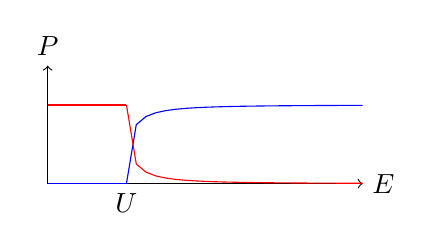
\begin{tikzpicture}[domain=-4:7] [scale=0.8]
\draw[->] (0,0) -- (4,0) node[right] {$E$};
\draw[->] (0,0) -- (0,1.5) node[above] {$P$};
\draw[color=red] plot[domain=0:1] (\x,{1 )});
\draw[color=blue] plot[domain=0:1] (\x,{0)});
\draw[color=blue] plot[domain=1:4] (\x,{4*sqrt(\x)*sqrt(\x-1)/(sqrt(\x)+sqrt(\x-1))^2) )});
\draw[color=red] plot[domain=1:4] (\x,{(sqrt(\x)-sqrt(\x-1))^2/(sqrt(\x)+sqrt(\x-1))^2) )});
\draw (1,0) node[below]{$U$};
\end{tikzpicture}
\end{center}
\end{eg}
\begin{eg}[Potential barrier]
   $$
V(x)=
\left\{
        \begin{array}{ll}
      U & 0<x<a\\
	0& x\leq 0,x\geq a\\
        \end{array}
    \right.
$$
Define $E$ and $U$ the same and consider $0<E<U$. We guess a wavefunction of the form
       $$
\psi(x)=
\left\{
        \begin{array}{ll}
      Ie^{ikx}+Re^{-ikx} & x<0\\
 Te^{ikx}& x>0\\
 Ae^{\kappa x}+Be^{-\kappa x}&0<x<a
        \end{array}
    \right.
$$
Invoke continuity condition of $\psi$ and $\psi'$ at $x=0$ and $x=a$ gives
$$I+R=A+B,\quad ik(I-R)=k(A-B)$$
$$Ae^{\kappa a}+Be^{-\kappa a}=Te^{ika},\quad \kappa (Ae^{\kappa a}-Be^{-\kappa a})=ikTe^{ika}$$
Solve them to get 
$$I+\frac{\kappa\mp ik}{\kappa\pm ik}R=Te^{ika}e^{\mp\kappa a}\implies T=Ie^{-ika}\frac{1}{\cosh\kappa a-i\frac{k^2-\kappa^2}{2k\kappa}\sinh ka}$$
The currents would be 
       $$
J(x)=
\left\{
        \begin{array}{ll}
      J_{inc}+J_{ref}=\frac{\hbar k}{m}(|I|^2-|R|^2)& x<0\\
J_{tr}=|T|^2\frac{\hbar k}{m}& x>0\\
        \end{array}
    \right.
$$
and thus 
$$P_{tr}=\frac{|J_{tr}|}{|J_{inc}|}=\frac{|T|^2}{|I|^2}=\frac{1}{1+\frac{U^2\sinh^2\kappa a}{4E(U-E)}}$$
This is the phenomenon of quantum tunnelling where there is non-zero probability of passing through the barrier even though it classically does not have enough energy. For $\kappa a>>1$, the probability decays as $e^{-2\kappa a}$.
\end{eg}
\begin{eg}[Infinite potential well]
Consider the following potential:
    $$
V(x)=
\left\{
        \begin{array}{ll}
      0 & |x|\leq a \\
	\infty& |x|>a\\
        \end{array}
    \right.
$$
$\psi=0$ at $|x|>a$. The boundary condition is $\psi$ continuous at $x=\pm a$, so $\psi(x=\pm a)=0$. At $x|<a$, 
$$\psi''+k^2\psi=0\implies\psi=A\cos kx+B\sin kx$$
The boundary condition gives $A\cos ka\pm B\sin ka=0\implies A\cos ka=B\sin ka=0$, which gives either $A=0\implies ka=p\pi$, $p\in\mathbb{Z}^+$ or $B=0\implies ka=(m-0.5)\pi$, $m\in\mathbb{Z}^+$. The wavefunctions will be
$$\psi_n(x)=\frac{1}{\sqrt{a}}\cos\frac{n\pi x}{2a}~n\text{ odd},\quad\frac{1}{\sqrt{a}}\sin\frac{n\pi x}{2a}~n\text{ even}$$
and satisfy the property $\psi_n(-x)=(-1)^{n+1}\psi_n(x)$. The energy eigenvalue is $E_n=\frac{\hbar^2\pi^2n^2}{8ma^2}$.
\end{eg}
\begin{prop}[Parity]
For symmetric potentials $V(x)=V(-x)$, we can just look for solutions with definite parity (purely even or purely odd).
\end{prop}
\begin{remarks}
To be specific, if $\psi(x)$ and $\psi(-x)$ represent the same quantum state, i.e. $\psi(-x)=\eta\psi(x)$, then $\psi(x)=\eta^2\psi(x)\implies\eta^2=1\implies\eta=\pm1$. If, however, they do not represent the same state, we can take a linear combination of it
$$\psi_\pm(x)=\alpha(\psi(x)\pm\psi(-x))$$
By construction, $\psi_\pm(-x)=\pm\psi_\pm(x)$ also have the same energy $E$.
\end{remarks}
\begin{eg}[Finite potential well]
   $$
V(x)=
\left\{
        \begin{array}{ll}
      -U & |x|\leq a \\
	0& |x|>a\\
        \end{array}
    \right.
$$
with $U$ a fixed constant. We seek solutions for
$$H\psi=-\frac{\hbar^2}{2m}\psi''+V(x)\psi=E\psi,\quad\text{for}-U<E<0$$
We can set $U+E=\frac{\hbar^2k^2}{2m}>0$ and $E=-\frac{\hbar^2\kappa^2}{2m}$. For $k,\kappa\in\mathbb{R}^+$ constants, then
$$\kappa^2+k^2=\frac{2mU}{\hbar^2}$$ 
Then, the Schr\"{o}dinger's equation becomes $\psi''+k^2\psi=0$ and $\psi''-\kappa^2\psi=0$ for $|x|<a$ and $|x|>a$ respectively. The boundary condition is to require $\psi$ and $\psi'$ to be continuous at $x=\pm a$.\\[5pt]
We first look for even parity solutions, i.e. $\psi(-x)=\psi(x)$.
   $$
\psi(x)=
\left\{
        \begin{array}{ll}
      A\cos kx & |x|\leq a \\
	Be^{-\kappa|x|}& |x|>a\\
        \end{array}
    \right.
$$
The boundary condition at $x=a$ (that of $x=-a$ will not give any new information) gives
$$A\cos ka=Be^{-\kappa a},\quad -Ak\sin ka=-\kappa Be^{-\kappa a}$$
which is essentially $k\tan ka=\kappa$. Together with the conservation of energy constraint $U+E=\frac{\hbar^2k^2}{2m}$, we have
$$(ak)^2+(a\kappa)^2=\frac{2ma^2U}{\hbar^2}$$
Plot this together with $a\kappa=ak\tan(ak)$.
\begin{center}
\begin{tikzpicture}[domain=-4:7] [scale=0.8]
\draw[->] (0,0) -- (7.5,0) node[right] {$ak$};
\draw[->] (0,0) -- (0,3.5) node[above] {$a\kappa$};
\draw[color=blue] plot[domain=0:1.3] (\x,{tan(deg(\x) )});
\draw[color=blue] plot[domain=3.14:4.45] (\x,{tan(deg(\x) )});
\draw[color=blue] plot[domain=6.28:7.5] (\x,{tan(deg(\x) )});
\draw [red, dashed] (1.5, 0) arc (0:90:1.5);
\draw [red, dashed] (3, 0) arc (0:90:3);
\draw (3.14,0) node[below]{$\pi$};
\draw (6.28,0) node[below]{$2\pi$};
\end{tikzpicture}
\end{center}
In particular, if $(n-1)\pi<\sqrt{2mU}\frac{a}{\hbar}<n\pi$, there are exactly $n$ even parity solutions for $n\geq1$. There is at least one even parity solution, which is the ground state. We next look for odd parity solutions, i.e. $\psi(-x)=-\psi(x)$.
   $$
\psi(x)=
\left\{
        \begin{array}{ll}
      A\sin kx & |x|\leq a \\
	Be^{-\kappa|x|}& |x|>a\\
        \end{array}
    \right.
$$
The boundary condition at $x=a$ (that of $x=-a$ will not give any new information) gives
$$A\sin ka=Be^{-\kappa a},\quad Ak\cos ka=-\kappa Be^{-\kappa a}$$
which is essentially $k\cot ka=\kappa$. Again, together with the conservation of energy constraint $(ak)^2+(a\kappa)^2=\frac{2ma^2U}{\hbar^2}$, we plot with $-a\kappa=ak \cot(ak)$. An odd parity solution may not exist if $ak<\frac{\pi}{2}$.
\begin{center}
\begin{tikzpicture}[domain=-4:7] [scale=0.8]
\draw[->] (0,0) -- (7.5,0) node[right] {$ak$};
\draw[->] (0,0) -- (0,3.5) node[above] {$a\kappa$};
\draw[color=blue] plot[domain=1.57:2.85] (\x,{-cot(deg(\x) )});
\draw[color=blue] plot[domain=4.7:5.98] (\x,{-cot(deg(\x) )});
\draw [red, dashed] (3, 0) arc (0:90:3);
\draw [red, dashed] (1, 0) arc (0:90:1);
\draw (1.57,0) node[below]{$\pi/2$};
\draw (4.7,0) node[below]{$3\pi/2$};
\end{tikzpicture}
\end{center}
For $E>0$ or $E<-U$, we get non-normalizable solutions. $-U<E<0$ is classically allowed. While quantum mechanically bounded in the potential, there is a non-zero probability of finding it outside the well. There is a discrete finite set of allowed energies. The transmission and reflected probabilities are plotted below as a function of energy $E$:
\begin{figure}[H]
\includegraphics[scale=0.5]{finitetransmission}
\centering
\caption{Transmission and Reflection Probability for Finite Square Well, where $|V_0|=1$}
\end{figure}
\end{eg}
\begin{eg}[Dirac potential well]
Consider the potential
$$ V(x)=-\alpha\delta(x)$$
We first examine bound states, where $E<0$. $\psi(x)$ is continuous everywhere, including $x=0$. But, its first derivative is discontinuous at $x=0$. The wavefunction for $|x|>0$ is a plane wave, $\psi(x)=Ae^{\kappa|x|}$ since there is no potential. For the discontinuous region, we will integrate the Schr\"{o}dinger Equation, from $-\epsilon$ to $\epsilon$ and then take the limit of $\epsilon$ approaching zero.
\begin{eqnarray}
\frac{-\hbar^2}{2m}\int_{-\epsilon}^{\epsilon}\frac{d^2\psi}{dx^2}dx-\int_{-\infty}^{\infty}\alpha\delta(x)\psi(x)dx&=&E\int_{-\infty}^{\infty}\psi(x)dx\nonumber\\\frac{-\hbar^2}{2m}\bigg(\frac{d\psi}{dx}\bigg\vert_{+\epsilon}-\frac{d\psi}{dx}\bigg\vert_{-\epsilon}\bigg) &=&-\lim_{\epsilon\to0}\int_{-\epsilon}^{\epsilon}\alpha\delta(x)\psi(x)dx+0\nonumber
\end{eqnarray}
We thus get $\kappa=\frac{m\alpha}{\hbar^2}$. The allowed energy is thus $E=-\frac{\hbar^2\kappa^2}{2m}=-\frac{m\alpha^2}{2\hbar^2}$. Normalizing the wavefunction will yield $A=\sqrt{\kappa}$. Hence,
$$
\psi(x)=\frac{\sqrt{m\alpha}}{\hbar}e^{-\frac{m\alpha|x|}{\hbar^2}}
$$
The Delta potential well thus has exactly one bound state, regardless of the height of the potential (characterized by $\alpha$). Suppose we have n number of Delta potential wells (with equal height $\alpha$) in a region $-L\leq x\leq L$, the wavefunction will have no nodes outside this region and there will only be at most one node in between each Delta potential (the actual number of nodes depends on magnitude of $\alpha$). There can only be at most $n$ bound states since there is a maximum number of $n-1$ nodes. Bear in mind that the ground state has no nodes.\\[5pt]
Next, we consider scattering states (wave incident from the left) where $E>0$. Setting $k=\frac{\sqrt{2mE}}{\hbar}$, the wavefunction is
$$
\psi(x)=
\left\{
        \begin{array}{ll}
      Ae^{ikx}+Be^{-ikx} & x<0 \\
	Fe^{ikx}& x>0\\
        \end{array}
    \right.
$$
The same boundary conditions apply. Former yields $A+B=F$ while latter yields $\frac{d\psi}{dx}|_{+}=ikF$ and 
$\frac{d\psi}{dx}|_{-}=ik(A-B)$. 
Using $\psi(0)=A+B$ and $\frac{-\hbar^2}{2m}(\frac{d\psi}{dx}\vert_{+\epsilon}-\frac{d\psi}{dx}\vert_{-\epsilon})=-\alpha\psi(0)$, we will get
$$ik(F-A+B)=-\frac{2m\alpha}{\hbar^2}(A+B)
$$
The reflection and transmission probabilities are
$$
|R|^2=\frac{|B|^2}{|A|^2}=\frac{(\frac{m\alpha}{\hbar^2k})^2}{1+(\frac{m\alpha}{\hbar^2k})^2}=\frac{1}{1+\frac{2\hbar^2E}{m\alpha^2}},\quad |T|^2=\frac{|F|^2}{|A|^2}=\frac{1}{1+(\frac{m\alpha}{\hbar^2k})^2}=\frac{1}{1+\frac{m\alpha^2}{2\hbar^2E}}
$$
The higher the energy, the greater the probability of transmission (blue), which is correct. 
\begin{center}
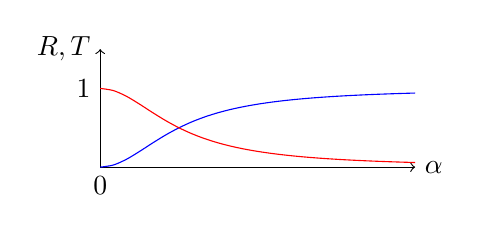
\begin{tikzpicture}
      \draw[->] (0,0) -- (4,0) node[right] {$\alpha$};
      \draw[->] (0,0) -- (0,1.5) node[left] {$R,T$};
      \draw[domain=0:4,smooth,variable=\x,blue] plot ({\x},{\x^2/(\x^2+1)});
      \draw[domain=0:4,smooth,variable=\x,red] plot ({\x},{1/(\x^2+1))});
      \draw (0,0) node[below]{0};
\draw (0,1) node[left]{1};
\end{tikzpicture}
\hfill
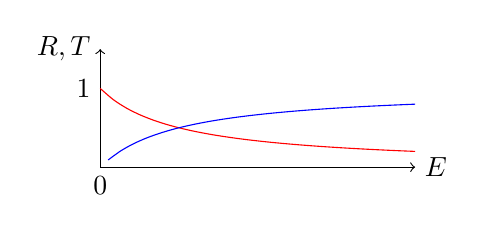
\begin{tikzpicture}
      \draw[->] (0,0) -- (4,0) node[right] {$E$};
      \draw[->] (0,0) -- (0,1.5) node[left] {$R,T$};
      \draw[domain=0:4,smooth,variable=\x,red] plot ({\x},{1/(\x+1)});
      \draw[domain=0.1:4,smooth,variable=\x,blue] plot ({\x},{1/((1/\x)+1))});
      \draw (0,0) node[below]{0};
\draw (0,1) node[left]{1};
\end{tikzpicture}
\end{center}
\end{eg}
\subsubsection*{Quantum Harmonic Oscillator}
\begin{note}[Series solution method]
The Schr\"{o}dinger's equation is
$$H\psi=-\frac{\hbar^2}{2m}\psi''+\frac{1}{2}m\omega^2x^2\psi=E\psi$$
We substitute $y=\sqrt{\frac{m\omega}{\hbar}}x$ and $\mathcal{E}=\frac{2E}{\hbar\omega}$ to obtain a cleaner form
$$-\frac{d^2\psi}{dy^2}+y^2\psi=\mathcal{E}\psi$$
For large $y,y^2>>\mathcal{E}$, try $\psi\propto e^{-y^2/2}$ so $\psi''$ can offset the large $y^2\psi$. Without loss of generality, set $\psi=f(y)e^{-y^2/2}$, then $f(y)$ satisfies the Hermite's equation
$$\frac{d^2f}{dy^2}-2y\frac{df}{dy}+\mathcal{E}-1=0$$
Try the series solution $f(y)=\sum_{r\geq0}a_ry^r$, then we obtain the recurrence relation:
$$a_{r+2}=\frac{2r+1-\mathcal{E}}{(r+2)(r+1)}a_r,\quad r\geq0$$
Choose $a_0$ and $a_1$ independently to get two linearly independent solutions. What is the behaviour of $f(y)$ when $y$ is large? If the coefficients do not vanish, $\frac{a_p}{a_{p-2}}\sim\frac{1}{p}$. This matches the coefficients of $y^\alpha e^{y^2}$ for some $\alpha$ and this gives $\psi\sim e^{y^2/2}$ which is not normalizable. Thus to ensure normalizability, we require the series $f$ to terminate. For this to do so, $\mathcal{E}=2n+1$ for some $n$. For each $n$, only one of the two independent solutions is normalizable. So for each $\mathcal{E}$, we get exactly one solution, so $f(y)=h_n(y)$ is a polynomial of degree $n$ with the property $h_n(-y)=(-1)^nh_n(y)$. These are Hermite polynomials. The solutions of the harmonic oscillator are
$$\psi_n(x)=h_n(\sqrt{m\omega/\hbar}x)\exp(-m\omega x^2/2\hbar)$$
with energy eigenvalues
$$E_n=\hbar\omega(n+0.5),\quad n\in\mathbb{Z}^+\cup\{0\}$$
The normalization fixes $a_0$ and $a_1$.
\end{note}
\newpage
\begin{note}[Operator method]
Inspired by classical case, we take the Hamiltonian (in operator form) of the harmonic oscillator to be
$$\hat{H}=\frac{1}{2m}\hat{p}^2+\frac{1}{2}m\omega^2\hat{x}^2,\quad \omega\in\mathbb{R},~m\in\mathbb{R}$$
To analyze this, begin by introducing the dimensionless operators
$$\hat{a}:=\frac{1}{\sqrt{2m\hbar\omega}}(m\omega\hat{x}+i\hat{p}),\quad\hat{a}^\dag:=\frac{1}{\sqrt{2m\hbar\omega}}(m\omega\hat{x}-i\hat{p})$$
which are called lowering and raising operators respectively. Then, we define the number operator $\hat{n}$ to be
$$\hat{n}:=\hat{a}^\dag\hat{a}=\frac{\hat{H}}{\hbar\omega}-0.5\implies\hat{H}=\hbar\omega(\hat{n}+0.5)$$
Observe that $\hat{n}$ is Hermitian. The raising and lowering operators commute with themselves but 
$$[\hat{a},\hat{a}^\dag]=\frac{1}{2m\hbar\omega}(m^2\omega^2[\hat{x},\hat{x}]+[\hat{p},\hat{p}]-im\omega[\hat{x},\hat{p}]+im\omega[\hat{p},\hat{x}])=1$$
where we used $[\hat{x},\hat{p}]=i\hbar$. Similarly, $[\hat{a}^\dag,\hat{a}]=-1$. We will also need $$[\hat{n},\hat{a}]=[\hat{a}^\dag\hat{a},\hat{a}^\dag]=\hat{a}^\dag[\hat{a},\hat{a}^\dag]+[\hat{a}^\dag,\hat{a}^\dag]\hat{a}=\hat{a}^\dag$$
Similarly, $[\hat{n},\hat{a}]=-\hat{a}$. Let the eigenstates be such that $|n\rangle$ with $\hat{n}|n\rangle=n|n\rangle$ and $\langle n|n\rangle=1$. Then, consider $\hat{a}^\dag|n\rangle$,
$$\hat{n}(\hat{a}^\dag|n\rangle)=([\hat{n},\hat{a}^\dag]+\hat{a}^\dag\hat{n})|n\rangle=(\hat{a}^\dag+\hat{a}^\dag\hat{n})|n\rangle=(n+1)|n+1\rangle$$
Similarly, $\hat{n}(\hat{a}|n\rangle)=(n-1)|n-1\rangle$. If $\hat{a}^\dag|n\rangle\neq0$, then $\hat{a}^\dag|n\rangle$ is also an eigenstate of $\hat{n}$ with eigenvalue $n+1$. If $\hat{a}|n\rangle\neq0$, then $\hat{a}|n\rangle$ is an eigenstate of $\hat{n}$ with eigenvalue $n-1$. Consequently, provided we can find some $|n\rangle$, we will construct a possibly infinite set of eigenstates of energies $E_k=(n+k+0.5)\hbar\omega$ for some $k\in\mathbb{Z}$ by acting repeatedly with $\hat{a}^\dag$ or $\hat{a}$. We can't yet conclude the energies are quantized, because we only know $n\in\mathbb{R}$. To go further, we investigate the norm
$$n=n\langle n|n\rangle=\langle n|\hat{n}|n\rangle=\langle n|\hat{a}^\dag\hat{a}|n\rangle=||\hat{a}|n\rangle||^2\geq0$$
With equality iff $\hat{a}|n\rangle=0$, i.e. $\hat{a}$ annihilates the state. Thus, all eigenvalues of $\hat{n}$ are non-negative, for any eigenstate $n\rangle\in\mathcal{H}$. We have just seen that if $\hat{a}|n\rangle\neq0$, it is an eigenstate of $\hat{n}$ with eigenvalue $n-1$. This lowering process must terminate. This will be the case iff $n\in\mathbb{N}_0$. Consequently, we have a ground state $|0\rangle$ defined by $\hat{a}|0\rangle=0$ and excited states $\sim(\hat{a}^\dag)^n|0\rangle$. The spectrum of $H$ is $E_n=(n+0.5)\hbar\omega$, $n\in\mathbb{N}_0$.\\[5pt]
We can recover the position space wavefunction of ground state as follow. We have 
$$0=\langle x|\hat{a}|0\rangle=\frac{1}{\sqrt{2m\hbar\omega}}\langle x|m\omega\hat{x}+i\hat{p}|0\rangle=\frac{1}{\sqrt{2m\hbar\omega}}\bigg(m\omega x+\hbar\frac{d}{dx}\bigg)\psi_0(x)$$
where $\langle x|0\rangle=\psi_0(x)$. This is a first order DE for $\psi_0(x)$ such that $\psi_0(x)=Ce^{-m\omega x^2/2\hbar}$. The $x$-space wavefunctions of excited states are likewise obtained from
$$\langle x|\hat{a}^\dag|0\rangle=\frac{1}{\sqrt{2m\hbar\omega}}\langle x|m\omega\hat{x}-i\hat{p}|0\rangle=\frac{C}{\sqrt{2m\hbar\omega}}\bigg(m\omega x-\hbar\frac{d}{dx}\bigg)e^{-m\omega x^2/(2\hbar)}$$
Careful. Although $\hat{a}^\dag|n\rangle$ is directly proportional to $|n+1\rangle$. It may not be correctly normalized. Indeed, we have
$$||\hat{a}^\dag|n\rangle||^2=\langle n|\hat{a}\hat{a}^\dag|n\rangle=\langle n|\hat{n}+[\hat{a},\hat{a}^\dag]|n\rangle=n+1$$
where $\langle n|n\rangle=1$. Likewise, $\hat{a}|n\rangle=\sqrt{n}|n-1\rangle$, and in particular, $\hat{a}|0\rangle=0$. We thus have
$$|n+1\rangle=\frac{(\hat{a}^\dag)^n}{\sqrt{(n+1)!}}|0\rangle$$
\end{note}
\begin{figure}[H]
\includegraphics[scale=0.75]{Hermite}
\centering
\caption{First few Hermite Polynomials}
\label{Hermite}
\end{figure}
\begin{figure}[H]
\includegraphics[scale=0.75]{oscillator2}
\centering
\caption{Energy Spectrum of Harmonic Oscillator}
\label{oscillator2}
\end{figure}
The $n$th energy eigenstate has $n$ nodes. Since the harmonic oscillator potential is quadratic and is even, the energy eigenstates are alternately even and odd, where the ground state is even. We can write the position and momentum in terms of the ladder operators
$$\mathbf{\hat{x}}=\sqrt{\frac{\hbar}{2m\omega}}(\mathbf{\hat{a}}+\mathbf{\hat{a}^\dag}),\quad \mathbf{\hat{p}}=i\sqrt{\frac{m\omega\hbar}{2}}(-\mathbf{\hat{a}}+\mathbf{\hat{a}^\dag})
$$
Using these two relations, we can calculate the expectation values for position and momentum (and squared) of the $n$th energy eigenstate. 
$$
\big\langle\psi_n|\mathbf{\hat{x}}|\psi_n\big\rangle=\sqrt{\frac{\hbar}{2m\omega}}\big\langle\psi_n|(\mathbf{\hat{a}}+\mathbf{\hat{a}^\dag})|\psi_n\big\rangle=0
$$
$$
\big\langle\psi_n|\mathbf{\hat{p}}|\psi_n\big\rangle=i\sqrt{\frac{m\omega\hbar}{2}}\big\langle\psi_n|(-\mathbf{\hat{a}}+\mathbf{\hat{a}^\dag})|\psi_n\big\rangle=0
$$
$$
\big\langle\psi_n|\mathbf{\hat{x}^2}|\psi_n\big\rangle=\frac{\hbar}{2m\omega}\big\langle\psi_n|(\mathbf{\hat{a}}+\mathbf{\hat{a}^\dag})^2|\psi_n\big\rangle=\frac{\hbar}{2m\omega}\big\langle\psi_n|(\mathbf{\hat{a}}\mathbf{\hat{a}^\dag}+\mathbf{\hat{a}^\dag}\mathbf{\hat{a}})|\psi_n\big\rangle=\frac{\hbar}{m\omega}(n+\frac{1}{2})$$
$$
\big\langle\psi_n|\mathbf{\hat{p}^2}|\psi_n\big\rangle=-\frac{m\omega\hbar}{2}\big\langle\psi_n|(-\mathbf{\hat{a}}+\mathbf{\hat{a}^\dag})^2|\psi_n\big\rangle=\frac{m\omega\hbar}{2}\big\langle\psi_n|(\mathbf{\hat{a}}\mathbf{\hat{a}^\dag}+\mathbf{\hat{a}^\dag}\mathbf{\hat{a}})|\psi_n\big\rangle=m\omega\hbar(n+\frac{1}{2})$$
The expectation values for kinetic energy  and potential energy are respectively
$$\big\langle K\big\rangle=\frac{1}{2m}\big\langle p^2 \big\rangle=\frac{1}{2}\hbar\omega(n+\frac{1}{2}),\quad\big\langle V\big\rangle=\frac{1}{2}m\omega^2\big\langle x^2 \big\rangle=\frac{1}{2}\hbar\omega(n+\frac{1}{2})$$
Hence, the expectation value of the Hamiltonian is  $\hbar\omega(n+\frac{1}{2})$. In fact, the Harmonic Oscillator obeys the Heisenberg Uncertainty Relation.
$$
\sigma_x\sigma_p=\sqrt{\frac{\hbar}{m\omega}(n+\frac{1}{2})-(0)^2}\sqrt{m\omega\hbar(n+\frac{1}{2})-(0)^2}=\hbar(n+0.5)\geq\frac{\hbar}{2}$$
The matrix representations for the ladder operators can be computed as follows:
$$
\langle n|\mathbf{\hat{a}}|m\rangle=\sqrt{m}\langle n|m-1\rangle=\sqrt{m}\delta_{n,m-1}
$$
$$
\langle n|\mathbf{\hat{a}}^\dag|m\rangle=\sqrt{m+1}\langle n|m+1\rangle=\sqrt{m+1}\delta_{n,m+1}
$$
The matrix representations for the position and momentum operator are
$$
\langle n|\mathbf{\hat{x}}|m\rangle=\sqrt{\frac{\hbar}{2m\omega}}(\sqrt{m}\delta_{n,m-1}+\sqrt{m+1}\delta_{n,m+1})
$$
$$
\langle n|\mathbf{\hat{p}}|m\rangle=i\sqrt{\frac{m\omega\hbar}{2}}(-\sqrt{m}\delta_{n,m-1}+\sqrt{m+1}\delta_{n,m+1})
$$
\begin{eqnarray}
\langle n|\mathbf{\hat{x}}^2|m\rangle&=&\sum_j\langle n|\mathbf{\hat{x}}|j\rangle\langle j|\mathbf{\hat{x}}|m\rangle\nonumber\\&=&\frac{\hbar}{2m\omega}\sum_j(\sqrt{j}\delta_{n,j-1}+\sqrt{j+1}\delta_{n,j+1})(\sqrt{m}\delta_{j,m-1}+\sqrt{m+1}\delta_{j,m+1})\nonumber\\&=&\frac{\hbar}{2m\omega}(\sqrt{m(m-1)}\delta_{n,m-2}+(2m+1)\delta_{n,m}+\sqrt{(m+1)(m+2)}\delta_{n,m+2})\nonumber
\end{eqnarray}
\begin{eqnarray}
\langle n|\mathbf{\hat{p}}^2|m\rangle&=&\sum_j\langle n|\mathbf{\hat{p}}|j\rangle\langle j|\mathbf{\hat{p}}|m\rangle\nonumber\\&=&-\frac{m\omega\hbar}{2}\sum_j(-\sqrt{j}\delta_{n,j-1}+\sqrt{j+1}\delta_{n,j+1})(-\sqrt{m}\delta_{j,m-1}+\sqrt{m+1}\delta_{j,m+1})\nonumber\\&=&-\frac{m\omega\hbar}{2}(\sqrt{m(m-1)}\delta_{n,m-2}-(2m+1)\delta_{n,m}+\sqrt{(m+1)(m+2)}\delta_{n,m+2})\nonumber
\end{eqnarray}
The matrix representation of the Hamiltonian will thus be
\begin{eqnarray}
\langle n|\mathbf{\hat{H}}^2|m\rangle&=&-\frac{\omega\hbar}{4}(\sqrt{m(m-1)}\delta_{n,m-2}-(2m+1)\delta_{n,m}+\sqrt{(m+1)(m+2)}\delta_{n,m+2})\nonumber\\&+&\frac{\hbar}{4}(\sqrt{m(m-1)}\delta_{n,m-2}+(2m+1)\delta_{n,m}+\sqrt{(m+1)(m+2)}\delta_{n,m+2})\nonumber\\&=&\hbar\omega\bigg(m+\frac{1}{2}\bigg)\delta_{n,m}\nonumber
\end{eqnarray}
Finally, the matrix representation of the number operator will be
$$
\langle n|\mathbf{\hat{N}}|m\rangle=\langle n|\mathbf{\hat{a}}^\dag\mathbf{\hat{a}}|m\rangle=\langle n|\mathbf{\hat{a}}^\dag\sqrt{m}|m-1\rangle=\langle n|\sqrt{m}\sqrt{m}|m\rangle=m\delta_{n,m}
$$
Note that no finite dimension representation of the position and momentum operators can replicate the commutation relation - $[\mathbf{\hat{x}},\mathbf{\hat{p}}]=i\hbar1$. The $4\times4$ truncated matrix representations will be
$$
\mathbf{\hat{x}}=\begin{bmatrix}0&1&0&0\\1&0&\sqrt{2}&0\\0&\sqrt{2}&0&\sqrt{3}\\0&0&\sqrt{3}&0\\\end{bmatrix}
$$
$$
\mathbf{\hat{p}}=\begin{bmatrix}0&-1&0&0\\1&0&-\sqrt{2}&0\\0&\sqrt{2}&0&-\sqrt{3}\\0&0&\sqrt{3}&0\\\end{bmatrix}
$$
The commutator will be
$$
[\mathbf{\hat{x}},\mathbf{\hat{p}}]=i\hbar\begin{bmatrix}1&0&0&0\\0&1&0&0\\0&0&1&0\\0&0&0&-3\\\end{bmatrix}\neq1
$$
\newpage
\begin{eg}[Coherent State]
Consider the family of coherent states of the harmonic oscillator:
$$|\alpha\rangle=e^{-|\alpha|^2/2}\sum_{n=0}^\infty\frac{\alpha^n}{\sqrt{n!}}|n\rangle$$
$|\alpha\rangle$ is clearly normalized but yet two coherent states are never orthogonal.
$$\langle\alpha|\alpha\rangle=e^{-|\alpha|^2}\sum_{m,n=0}^\infty\frac{(\alpha^*)^n\alpha^m}{\sqrt{n!m!}}\delta_{n,m}=1$$
$$\langle\alpha|\beta\rangle=e^{-(|\alpha|^2+|\beta|^2)/2}\sum_{m,n=0}^\infty\frac{(\alpha^*)^n\beta^m}{\sqrt{n!m!}}\delta_{n,m}=e^{-|\alpha-\beta|^2/2}e^{i\text{Im}(\alpha^*\beta)}\neq0$$
Interestingly, the coherent states are eigenvectors of $a$, but not $a^\dag$.
$$a|\alpha\rangle=e^{-|\alpha|^2/2}\sum_{n=0}^\infty\frac{\alpha^n}{\sqrt{n!}}a|n\rangle=e^{-|\alpha|^2/2}\sum_{n=1}^\infty\frac{\alpha^{n-1}\alpha}{\sqrt{(n-1)!}}|n-1\rangle=\alpha|\alpha\rangle$$
Suppose $a^\dag|\psi\rangle=\lambda|\psi\rangle$ has a solution. We can write $|\psi\rangle=\sum_nc_n|n\rangle$, then $a^\dag|\psi\rangle=\sum_nc_n\sqrt{n+1}|n+1\rangle$, then let $m$ be the smallest integer for which $c_m\neq 0$, then the vector $|\psi\rangle$ have a component along $|m\rangle$, while $a^\dag|\psi\rangle$ has not, hence linearly independent from $|\psi\rangle$, $\forall|\psi\rangle$, hence contradict. Now, for the expectation value:
$$\alpha=\langle\alpha|a|\alpha\rangle=\sqrt{\frac{m\omega}{2\hbar}}\langle\alpha|x|\alpha\rangle+\frac{i}{\sqrt{2m\hbar\omega}}\langle\alpha|p|\alpha\rangle$$
and so $\langle x\rangle_\alpha=\sqrt{\frac{2\hbar}{m\omega}}\text{Re}(\alpha)$ and $\langle p\rangle_\alpha=\sqrt{2m\hbar\omega}\text{Im}(\alpha)$. Interestingly, we can solve for the coherent state in the position representation, i.e. $a\psi_\alpha(x)=\alpha\psi_\alpha(x)$ and we get a form
$$\psi_\alpha(x)=Ae^{-\frac{m\omega}{2\hbar}(x-x_0)^2}e^{ik_0x}$$
where $A$ is some constant, which has a Gaussian form. Note that only $|\alpha=0\rangle$ coincides with $|n=0\rangle$, all other coherent states are a superposition of all the eigenstates of $H$ and they can't be states of well-defined energy and so
$$\langle H\rangle_\alpha=\sum_{n=0}^\infty \hbar\omega(n+0.5)e^{-|\alpha|^2}\frac{|\alpha|^{2n}}{n!}=\hbar\omega(|\alpha|^2+0.5)$$
We can also show for fixed $\langle x\rangle$ and fixed $\langle p\rangle$, the coherent state is a state that minimizes the value of $\langle N\rangle$, and hence minimizes the average value of the energy.
\end{eg}
\begin{eg}[Sudden change in potential]
Consider a potential $V=ax^2$, $x\geq 0$ but 0 when $x<0$. Then $\psi(x=0)=0$ and discontinuous first derivative at $x=0$. The ground state has to be $Bxe^{-Cx^2}$ for $x>0$, for some constants $B$ and $C$. Now if the particle in this potential, is in the ground state, and that the potential is suddenly changed to $ax^2$ $\forall x$. The new ground state will be $Ae^{-Cx^2}$ and the probability will be $\int_0^\infty B^*xe^{-Cx^2}Ae^{-Cx^2}dx$. 
\end{eg}
\begin{eg}[Heisenberg Operators]
The Heisenberg equation of motion yields $\frac{d}{dt}\hat{x}_H(t)=\frac{1}{m}\hat{p}_H(t)$ and $\frac{d}{dt}\hat{p}_H(t)=-m\omega^2\hat{x}_H(t)$. Setting $\hat{x}_H(t=0)=\hat{x}_S$ and $\hat{p}_H(t=0)=\hat{p}_S$,
$$\begin{bmatrix}\hat{x}_H(t)\\\hat{p}_H(t)\\\end{bmatrix}=\begin{bmatrix}\cos(\omega t)&(m\omega)^{-1}\sin(\omega t)\\\-m\omega\sin(\omega t)&\cos(\omega t)\\\end{bmatrix}\begin{bmatrix}\hat{x}_S\\\hat{p}_S\\\end{bmatrix}$$
Moreover, $\hat{a}_H(t)=e^{-i\omega t}\hat{a}_S$. 
\end{eg}
\begin{Note}[Morse Oscillator]
$V_M(r)=D_e(1-e^{-\beta(r-r_e)})^2$, where $D_e$ is the dissociation energy, $r_e$ is equilibrium bond length. Expanding as power series, we get a force constant $k=2\beta^2D_e$. Interestingly, the Morse potential can be solved exactly with energy $E_n=(n+0.5)\hbar\omega-(n+0.5)^2\hbar\omega x_e$, where $x_e=\frac{\hbar\beta^2}{2m\omega}=\frac{\hbar\omega}{4D_e}$ is the anharmonicity constant.
\end{Note}
\newpage
\subsection{3D Problems}
\subsubsection*{Orbital Angular Momentum}
\begin{defi}[Orbital Angular Momentum]
Classically,  $\mathbf{L}=\mathbf{r}\times\mathbf{p}=\epsilon_{ijk}x_ip_j\mathbf{\hat{k}}$. The corresponding quantum mechanial definition is
$$\mathbf{\hat{L}_i}=-i\hbar\epsilon_{jki}\mathbf{\hat{x}_j}\frac{\partial}{\partial x_k}$$
\end{defi}
\begin{defi}[Total Angular Momentum]
The total angular momentum is
$$\mathbf{\hat{L}^2}=\mathbf{\hat{L}_i}\mathbf{\hat{L}_i}$$
\end{defi}
\begin{thm}[Angular Momentum operators in Spherical Coordinates]
$$\mathbf{\hat{L}_x}=i\hbar\bigg(\cos\phi\cot\theta\frac{\partial}{\partial\phi}+\sin\phi\frac{\partial}{\partial\theta}\bigg),\quad\mathbf{\hat{L}_y}=i\hbar\bigg(\sin\phi\cot\theta\frac{\partial}{\partial\phi}+\cos\phi\frac{\partial}{\partial\theta}\bigg)$$
$$\mathbf{\hat{L}_z}=-i\hbar\frac{\partial}{\partial\phi},\quad\mathbf{\hat{L}^2}=-\hbar^2\bigg(\frac{1}{\sin\theta}\frac{\partial}{\partial\theta}\bigg(\sin\theta\frac{\partial}{\partial\theta}\bigg)+\frac{1}{\sin^2\theta}\frac{\partial^2}{\partial\phi^2}\bigg)$$
\end{thm}
\begin{proof}
We have $x=r\sin\theta\cos\phi$, $y=r\sin\theta\sin\phi$, $z=r\cos\theta$ so by chain rule
$$\frac{\partial}{\partial\theta}=\frac{\partial x}{\partial\theta}\frac{\partial}{\partial x}+\frac{\partial y}{\partial\theta}\frac{\partial}{\partial y}+\frac{\partial z}{\partial\theta}\frac{\partial}{\partial z}=r\cos\theta\cos\phi\frac{\partial}{\partial x}+r\cos\theta\sin\phi\frac{\partial}{\partial y}-r\sin\theta\frac{\partial}{\partial z}$$
$$\frac{\partial}{\partial\phi}=\frac{\partial x}{\partial\phi}\frac{\partial}{\partial x}+\frac{\partial y}{\partial\phi}\frac{\partial\phi}{\partial y}=-r\sin\theta\sin\phi\frac{\partial}{\partial x}+r\sin\theta\cos\phi\frac{\partial}{\partial y}$$
From the definition of orbital angular momentum, we have
$$\mathbf{\hat{L}_x}=-i\hbar\bigg(y\frac{\partial}{\partial z}-z\frac{\partial}{\partial y}\bigg)=i\hbar\bigg(\cos\phi\cot\theta\frac{\partial}{\partial\phi}+\sin\phi\frac{\partial}{\partial\theta}\bigg)$$
$$\mathbf{\hat{L}_y}=-i\hbar\bigg(z\frac{\partial}{\partial x}-x\frac{\partial}{\partial z}\bigg)=i\hbar\bigg(\sin\phi\cot\theta\frac{\partial}{\partial\phi}+\cos\phi\frac{\partial}{\partial\theta}\bigg)$$
$$\mathbf{\hat{L}_z}=-i\hbar\bigg(x\frac{\partial}{\partial y}-y\frac{\partial}{\partial x}\bigg)=-i\hbar\frac{\partial}{\partial\phi}$$
For $\mathbf{\hat{L}^2}$, we could either directly sum the squares or we could use this clever trick:
$$\hat{L}_\mp\hat{L}_\pm=(\hat{L}_x\mp i\hat{L}_y)(\hat{L}_x\pm i\hat{L}_y)=\hat{L}_x^2+\hat{L}_y^2\pm i[\hat{L}_x,\hat{L}_y]=\hat{L}_x^2+\hat{L}_y^2\mp\hbar\hat{L}_z=\hat{L}^2-\hat{L}_z^2\mp\hbar\hat{L}_z$$
Evaluating the commutator
$$[\hat{L}_+,\hat{L}_-]=-i[\hat{L}_x,\hat{L}_y]+i[\hat{L}_y,\hat{L}_x]=-ii\hbar\hat{L}_z+i(-i\hbar\hat{L}_z)=2\hbar\hat{L}_z$$
and 
\begin{eqnarray}
\hat{L}_\pm\hat{L}_\mp&=&\hbar^2e^{\pm i\phi}\bigg(\pm\frac{\partial}{\partial\theta}+i\cot\theta\frac{\partial}{\partial\phi}\bigg)e^{\mp i\phi}\bigg(\mp\frac{\partial}{\partial\theta}+i\cot\theta\frac{\partial}{\partial\phi}\bigg)\nonumber\\&=&\hbar^2e^{\pm i\phi}\frac{\partial}{\partial\theta}e^{\mp i\phi}\bigg(\mp\frac{\partial}{\partial\theta}+i\cot\theta\frac{\partial}{\partial\phi}\bigg)+e^{\pm i\phi}i\cot\theta\frac{\partial}{\partial\phi}e^{\mp i\phi}\bigg(\mp\frac{\partial}{\partial\theta}+i\cot\theta\frac{\partial}{\partial\phi}\bigg)\nonumber\\&=&\hbar^2\bigg(-\frac{\partial^2}{\partial\theta^2}\mp i\frac{\partial}{\partial\phi}-\cot\theta\frac{\partial}{\partial\theta}-\cot^2\theta\frac{\partial^2}{\partial\phi^2}\bigg)
\nonumber
\end{eqnarray}
Hence, $\hat{L}^2$ will be
$$\hat{L}^2=\hbar^2\bigg(-\frac{\partial^2}{\partial\theta^2}- i\frac{\partial}{\partial\phi}-\cot\theta\frac{\partial}{\partial\theta}-\cot^2\theta\frac{\partial^2}{\partial\phi^2}\bigg)-\hbar^2\frac{\partial^2}{\partial\phi^2}+i\hbar^2\frac{\partial}{\partial\phi}=-\hbar^2\bigg(\frac{1}{\sin\theta}\frac{\partial}{\partial\theta}\sin\theta\frac{\partial}{\partial\theta}+\frac{1}{\sin^2\theta}\frac{\partial^2}{\partial\phi^2}\bigg)$$
\end{proof}
\begin{thm}[Commutation Relation for Angular Momentum]
$$[\mathbf{\hat{L}_i},\mathbf{\hat{L}_j}]=i\hbar\epsilon_{ijk}\mathbf{\hat{L}_k},\quad [\mathbf{\hat{L}^2},\mathbf{\hat{L}_i}]=0$$
$$[\mathbf{\hat{L}_i},\mathbf{\hat{r}_j}]=i\hbar\epsilon_{ijk}\mathbf{\hat{r}_k},\quad[\mathbf{\hat{L}_i},\mathbf{\hat{p}_j}]=i\hbar\epsilon_{ijk}\mathbf{\hat{p}_k}$$
$$[\mathbf{\hat{L}_i},\sum_j\mathbf{\hat{r}_j}^2]=2i\hbar\epsilon_{ijk}\mathbf{\hat{r}_j}\mathbf{\hat{r}_k}=0,\quad[\mathbf{\hat{L}_i},\sum_j\mathbf{\hat{p}_j}^2]=2i\hbar\epsilon_{ijk}\mathbf{\hat{p}_j}\mathbf{\hat{p}_k}=0$$
\end{thm}
\begin{proof}
Using index notation,
$$[\hat{L}_i,\hat{r}_l]f=-i\hbar\epsilon_{jki}\bigg[\hat{r}_j\frac{\partial}{\partial r_k},\hat{r}_l\bigg]f=-i\hbar\epsilon_{jki}r_j\frac{\partial r_l}{\partial r_k}f=-i\hbar\epsilon_{jki}r_j\delta_{l,k}f\implies[\hat{L}_i,\hat{r}_k]=i\hbar\epsilon_{ikj}r_j$$
$$[\hat{L}_i,\hat{p}_l]f=-i\hbar\epsilon_{jki}\frac{\hbar}{i}\bigg[\hat{r}_j\frac{\partial}{\partial r_k},\frac{\partial}{\partial r_l}\bigg]f=-\epsilon_{jki}\hbar^2\bigg(r_j\frac{\partial}{\partial r_k}\bigg(\frac{\partial f}{\partial r_l}\bigg)-\frac{\partial}{\partial r_l}\bigg(r_j\frac{\partial f}{\partial r_k}\bigg)\bigg)=\hbar^2\epsilon_{jki}\frac{\partial }{\partial r_k}\delta_{j,l}$$
$$\implies[\hat{L}_i,\hat{p}_j]=i\hbar\epsilon_{ijk}\hat{p}_k$$
$$\hat{L}_i \hat{L}_j= \varepsilon_{iar} \hat{r}_a \hat{p}_r \varepsilon_{jbs} \hat{r}_b \hat{p}_s= \varepsilon_{iar} \varepsilon_{jbs} (\hat{r}_a \hat{p}_r \hat{r}_b \hat{p}_s)= \varepsilon_{iar} \varepsilon_{jbs} (\hat{r}_a (\hat{r}_b \hat{p}_r - [\hat{p}_r, \hat{r}_b]) \hat{p}_s)= \varepsilon_{iar} \varepsilon_{jbs} (\hat{r}_a \hat{r}_b \hat{p}_r \hat{p}_s - i\hbar \delta_{br} \hat{r}_a \hat{p}_s)$$
 \begin{align*}
        \implies[\hat{L}_i,\hat{L}_j] &= -i\hbar \varepsilon_{iar} \varepsilon_{jbs}(\delta_{br} \hat{r}_a \hat{p}_s - \delta_{as}\hat{r}_b \hat{p}_r)\\
        &= -i\hbar (\varepsilon_{iab} \varepsilon_{jbs}\hat{r}_a \hat{p}_s - \varepsilon_{iar} \varepsilon_{jba} \hat{r}_b\hat{p}_r)\\
        &= -i\hbar ((\delta_{is} \delta_{ja} - \delta_{ij} \delta_{as})\hat{r}_a \hat{p}_s - (\delta_{ib} \delta_{rj} - \delta_{ij}\delta_{rb}) \hat{r}_b \hat{p}_r)\\
        &= i\hbar (\hat{r}_i p_j - \hat{r}_j p_i)\\
        &= i\hbar \varepsilon_{ijk} L_k.
      \end{align*}
$$[\hat{L}_i,\hat{L}^2]=[\hat{L}_i,\hat{L}_j\hat{L}_j]=i\hbar\epsilon_{ijk}\hat{L}_k\hat{L}_j+\hat{L}_ji\hbar\epsilon_{ijk}\hat{L}_k=0$$
$$[\hat{L}_i,\hat{r}^2]=[\hat{L}_i,\hat{r}_j\hat{r}_j]=i\hbar\epsilon_{ijk}\hat{r}_k\hat{r}_j+\hat{r}_ji\hbar\epsilon_{ijk}\hat{r}_k=0$$
$$[\hat{L}_i,\hat{p}^2]=[\hat{L}_i,\hat{p}_j\hat{p}_j]=i\hbar\epsilon_{ijk}\hat{p}_k\hat{p}_j+\hat{p}_ji\hbar\epsilon_{ijk}\hat{p}_k=0$$
where the last three results are zero since for instance,  $\epsilon_{ijk}\hat{L}_k\hat{L}_j=-\epsilon_{kji}\hat{L}_k\hat{L}_j=\epsilon_{jki}\hat{L}_j\hat{L}_k$ after relabelling.
\end{proof}
\begin{defi}[Angular Momentum Ladder Operators]
The angular momentum ladder operators are defined to be
$$\mathbf{\hat{L}_{\pm}}=\mathbf{\hat{L}_x}\pm i\mathbf{\hat{L}_y}$$
\end{defi}
\begin{thm}
$$\mathbf{\hat{L}_{\mp}}\mathbf{\hat{L}_{\pm}}=\mathbf{\hat{L}^2}-\mathbf{\hat{L}_z^2}\mp\hbar\mathbf{\hat{L}_z}$$
\end{thm}
\begin{proof}
$$\mathbf{\hat{L}_{\mp}}\mathbf{\hat{L}_{\pm}}=\mathbf{\hat{L}_x}^2+\mathbf{\hat{L}_y}^2\pm i[\mathbf{\hat{L}_x},\mathbf{\hat{L}_y}]=\mathbf{\hat{L}^2}-\mathbf{\hat{L}_z^2}\mp\hbar\mathbf{\hat{L}_z}$$
\end{proof}
\begin{defi}[$l$ and $m$]
$l$ and $m$ are known as the Orbital Angular Momentum quantum number and Azimuthal quantum number respectively such that $\mathbf{\hat{L}_z}|l,m\rangle=\hbar m|l,m\rangle$ and $\mathbf{\hat{L}^2}|l,m\rangle=\hbar^2l(l+1)|l,m\rangle$.
\end{defi}
\begin{thm}
For $m=-l$, $\mathbf{\hat{L}_-}|l,m\rangle=0$. If $m>-l$, we obtain $|l,m-1\rangle$ after one iteration of $\mathbf{\hat{L}_-}$. Similarly, for $m=+l$, $\mathbf{\hat{L}_+}|l,m\rangle=0$. If $m<l$, we obtain $|l,m-1\rangle$.
\end{thm}
\begin{proof}
We have
$$||\mathbf{\hat{L}_{\pm}}|l,m\rangle||^2=\langle l,m|\mathbf{\hat{L}^2}-\mathbf{\hat{L}_z^2}\mp\hbar\mathbf{\hat{L}_z}|l,m\rangle=\hbar^2(l(l+1)-m^2\mp m)=\hbar^2(l\mp m)(l\pm m+1)$$
Both must be non-negative, so $-l-1\leq m\leq l$ and $-l\leq m\leq l+1$, and hence $-l\leq m\leq l$. Now, if $\mathbf{\hat{L}_-}|l,m\rangle=0$, then we can only have $m=-l$. If $m>-l$, then the resultant state is $|l,m-1\rangle$.
$$\mathbf{\hat{L}_z}\mathbf{\hat{L}_-}|l,m\rangle=\mathbf{\hat{L}_-}\mathbf{\hat{L}_z}|l,m\rangle-\hbar\mathbf{\hat{L}_-}|l,m\rangle=\hbar(m-1)|l,m-1\rangle$$
Similarly, $\mathbf{\hat{L}_+}|l,m=+l\rangle=0$ and if $m<l$, the resultant state is $|l,m+1\rangle$.
\end{proof}
\begin{thm}[Matrix Representations of Angular Momentum Operators]
$$\langle l',m'|\mathbf{\hat{L}^2}|l,m\rangle=\hbar^2l(l+1)\delta_{l',l}\delta_{m',m}$$
$$\langle l',m'|\mathbf{\hat{L}_z}|l,m\rangle=\hbar m\delta_{l',l}\delta_{m',m}$$
$$\langle l',m'|\mathbf{\hat{L}_x}|l,m\rangle=0.5\hbar[\sqrt{l(l+1)-m(m+1)}\delta_{m',m+1}+\sqrt{l(l+1)-m(m-1)}\delta_{m',m-1}]\delta_{j',j}$$
$$\langle l',m'|\mathbf{\hat{L}_y}|l,m\rangle=0.5\hbar[\sqrt{l(l+1)-m(m+1)}\delta_{m',m+1}-\sqrt{l(l+1)-m(m-1)}\delta_{m',m-1}]\delta_{j',j}$$
\end{thm}
\begin{proof}
For $\mathbf{\hat{L}^2}$ and $\mathbf{\hat{L}_z}$, it follows from definition. From the ladder operators, we have
$$\langle l',m'|\mathbf{\hat{L}_{\pm}}|l,m\rangle=\hbar\sqrt{l(l+1)-m(m\pm1)}\delta_{l',l}\delta_{m',m\pm1}$$
Then, the result follows from the definition of $\mathbf{\hat{L}_{\pm}}$.
\end{proof}
\begin{cor}
The expectation values of $\mathbf{\hat{L}_x}$ and $\mathbf{\hat{L}_y}$ are both zero. The expectation values for $\mathbf{\hat{L}_x^2}$ and $\mathbf{\hat{L}_y^2}$ are both $0.5\hbar^2(l(l+1)-m^2)$. Moreover,
$$\sigma_{L_x}\sigma_{L_y}\geq\frac{\hbar^2}{2}|\langle\mathbf{\hat{L}_z}\rangle|$$
\end{cor}
\begin{proof}
Since the eigenstates with different $m$ numbers are orthogonal to each other, the expectation values of $\mathbf{\hat{L}_x}$ and $\mathbf{\hat{L}_y}$ are both zero. Now,
$$\mathbf{\hat{L}_x^2}=\frac{1}{4}\langle(\mathbf{\hat{L}_+}^2+\mathbf{\hat{L}_+}\mathbf{\hat{L}_-}+\mathbf{\hat{L}_-}\mathbf{\hat{L}_+}+\mathbf{\hat{L}_-^2})\rangle=\frac{1}{4}\langle(\mathbf{\hat{L}_+}\mathbf{\hat{L}_-}+\mathbf{\hat{L}_-}\mathbf{\hat{L}_+})\rangle$$
$$\mathbf{\hat{L}_y^2}=-\frac{1}{4}\langle(\mathbf{\hat{L}_+}^2-\mathbf{\hat{L}_+}\mathbf{\hat{L}_-}-\mathbf{\hat{L}_-}\mathbf{\hat{L}_+}+\mathbf{\hat{L}_-^2})\rangle=\frac{1}{4}\langle(\mathbf{\hat{L}_+}\mathbf{\hat{L}_-}+\mathbf{\hat{L}_-}\mathbf{\hat{L}_+})\rangle=\mathbf{\hat{L}_x^2}=\frac{1}{2}\hbar^2[l(l+1)-m^2]$$
So, the product of uncertainties will be
$$\sigma_{L_x}\sigma_{L_y}=0.5\hbar^2[l(l+1)-m^2]\geq0.5\hbar^2[m(m+1)-m^2]=0.5\hbar^2m=\frac{\hbar^2}{2}|\langle\mathbf{\hat{L}_z}\rangle|$$
\end{proof}
\begin{Note}
Geometrically, the angular momentum vector $L$ traces out a cone in 3 dimensional angular momentum space where the length of the vector is $\hbar\sqrt{l(l+1)}$ and the half angle of the cone is $\cos^{-1}(m/\sqrt{l(l+1)})$.  $m$ is thus the projection of the angular momentum vector along the $z$ axis. As the angular momenta states are quantized, $\theta$ is quantized too and have a discrete set of $2l + 1$ possible values. As $l\rightarrow\infty$ (classical limit), $\theta\rightarrow 0$, this physically means we can measure the angular momentum's direction with great certainty.
\end{Note}
\begin{thm}
The common diagonalization of $\mathbf{\hat{L}^2}$ and $\mathbf{\hat{L}_z}$ yields:
\begin{itemize}
    \item The eigenvalues of $\mathbf{\hat{L}}^2$ are of the form $\hbar^2l(l+1)$ with $l$ integer or half-integer.
    \item For a given value of $l$, the eigenvalues of $\mathbf{\hat{L}_z}$ are $\hbar m$ with $m\in\{-l,-l+1,...,l-1,l\}$.
\end{itemize}
That is, the eigenvalue $l$ of $\mathbf{L}^2$ has a multiplicity of $2l+1$.
\end{thm}
\begin{proof}
Observe that the eigenvalues of $\mathbf{\hat{L}^2}$ are non-negative:
$$\langle\psi|\mathbf{\hat{L}^2}|\psi\rangle=||L_x|\psi\rangle||^2+||L_y|\psi\rangle||^2+||L_z|\psi\rangle||^2$$
Take an eigenvalue $\hbar m'$ of $\mathbf{\hat{L}_z}$. Just as with the harmonic oscillator, if $p=m'+l\notin\mathbb{Z}$, by subsequent applications of $\mathbf{\hat{L}_-}$, we would find a non-zero eigenvector with eigenvalue $m<-l$. Similarly, if $q=l-m'\notin\mathbb{Z}$, then by subsequent applications of $J_+$, we would find a non-zero eigenvector with eigenvalue $m>+l$. So $q+p=2l\in\mathbb{N}$, whence $l$ can only be integer or half-integer. The possible values of $m$ are indeed $\{-l,-l+1,...,l-1,l\}$.
\end{proof}
\begin{cor}
The family of simultaneous eigenfunctions of $\mathbf{\hat{L}^2}$ and $\mathbf{\hat{L}_z}$ is
$$Y_{l,m}(\theta,\phi)=P_{l,m}(\theta)e^{im\phi}$$
where $P_{l,m}(\theta)$ is the associated Legendre functions.
\end{cor}
\begin{proof}
By separation of variables, we seek solutions of the form $T(\theta)P(\phi)$. 
$$-iT\hbar P'=\hbar mTP\implies P=e^{im\phi}$$
As $\phi$ is defined modulo $2\pi$, we need $e^{im(\phi+2\pi)}=e^{im\phi}$ so $e^{i2m\pi}=1\implies m\in\mathbb{Z}$. Now, for $\mathbf{\hat{L}^2}$,
$$-\hbar^2\bigg(\frac{1}{\sin\theta}\frac{d}{d\theta}\bigg(\sin\theta\frac{d}{d\theta}\bigg)-\frac{m^2}{\sin^2\theta}\bigg)T=\hbar^2l(l+1) T\implies\sin\theta\frac{d}{d\theta}(\sin\theta T')+(l(l+1)\sin^2\theta-m^2)T=0$$
With the substitution $x=\cos\theta$,  $\sin\theta\frac{d}{d\theta}=-(1-x^2)\frac{d}{dx}$ and so we obtain the Legendre equation such that $T(\theta)$ is the associated Legendre functions $P_{m,l}(\cos\theta)$. For the case $m=0$, we can guess a polynomial solution for $P_l(x)$ and we get the following recurrence relation
$$a_{k+2}=a_k\frac{k(k+1)-l(l+1)}{(k+1)(k+2)}$$
For the series to terminate at the $k$th power, we set $k=l$. By the Rodriguez formula, $P_l(x)=\frac{1}{2^ll!}\frac{d^l}{dx^l}(x^2-1)^l$. It can then be shown that the associated Legendre functions can be expanded in terms of the ordinary Legendre polynomial
$$P_{m,l}(x)=(1-x^2)^{|m|/2}\bigg(\frac{d}{dx}\bigg)^{|m|}P_l(x)$$
Since the differential equation involves $m^2$, we can take solutions for $\pm m$ to be the same. Naturally, $|m|\leq l$ must be true, hence there are $2l+1$ possible integer values of $m$, as expected. Upon normalization, the common eigenfunction is
$$Y_{l,m}(\theta,\phi)=\sqrt{\frac{2l+1}{4\pi}\frac{(l-m)!}{(l+m)!}}(-1)^me^{im\phi}P_{m,l}(\cos\theta)$$
where $Y_{l,m}$ is known as the spherical harmonics.
\end{proof}
\begin{cor}
The parity of the eigenfunction depends on only $l$.
\end{cor}
\begin{proof}
The parity transformation on its position, i.e. $\theta'=\pi-\theta$ and $\phi'=\phi+\phi$. We then have $Y_{l,m}(\theta,\phi)\mapsto Y_{l,m}(\theta',\phi')=(-1)^lY_{l,m}(\theta,\phi)$.
\end{proof}
\begin{defi}[Rotational Invariant Quantity]
If a physical quantity $A$ is rotational invariant, it commutes with the angular momentum, i.e. $[\mathbf{\hat{A}},\mathbf{\hat{L}}]=0$.
\end{defi}
\begin{thm}[Generator of Rotations]
The unitary operator $e^{i\epsilon\mathbf{\hat{L}_z}/\hbar}$ corresponds to a clockwise rotation by an infinitesimal angle $\epsilon$ about the $z$ axis.
\end{thm}
\begin{proof}
Suppose we perform a clockwise rotation by an infinitesimal angle $\epsilon$ such that $x'\approx x(1-0.5\epsilon^2)-\epsilon y$ and $y'\approx y(1-0.5\epsilon^2)+\epsilon x$. Then we have $\psi(x-\epsilon y,y+\epsilon x)\approx\psi(x,y)-\epsilon y\frac{\partial}{\partial x}\psi+\epsilon x\frac{\partial}{\partial y}\psi$. 
$$e^{i\epsilon\mathbf{\hat{L}_z}/\hbar}\psi(x,y)\approx(1+\epsilon\mathbf{\hat{L}_z})\psi(x,y)=\bigg(1+\epsilon\bigg(x\frac{\partial}{\partial y}-y\frac{\partial}{\partial x}\bigg)\bigg)\psi(x,y)=\psi(x,y)-\epsilon y\frac{\partial\psi}{\partial x}+\epsilon x\frac{\partial\psi}{\partial y}$$
\end{proof}
\begin{remarks}
$\mathbf{L}$ is a Hermitian operator which is a generator of circular translations.
\end{remarks}
\subsubsection*{Schr\"{o}dinger Equation in 3D}
\begin{eg}[Rectangular Box Potential]
Consider the case of a spinless particle of mass $m$ confined in a rectangular box of sides $a$, $b$, $c$ such that $V(x,y,z)=0$ for $0<x<a$, $0<y<b$ and $0<z<c$ and infinity otherwise. The wavefunction will be
$$\psi_{n_x,n_y,n_z}(x,y,z)=\sqrt{\frac{8}{abc}}\sin(n_x\pi x/a)\sin(n_y\pi y/b)\sin(n_z\pi z/c)$$
with energy $E_{n_x,n_y,n_z}=\frac{\hbar^2\pi^2}{2m}(\frac{n_x^2}{a^2}+\frac{n_y^2}{b^2}+\frac{n_z^2}{c^2})$. Degeneracies exist at common multiples of at least two of the quantities in $\{\frac{n_x^2}{a^2},\frac{n_y^2}{b^2},\frac{n_z^2}c^2\}$. Now if $a=b=c$, we just require degeneracy for any combination of $(n_x,n_y,n_z)$ such that $n_x^2+n_y^2+n_z^2$ is a constant, hence giving the same energy.
\end{eg}
\begin{eg}
Consider a spinless particle of mass $m$ in a 3D potential $V(x,y,z)=0.5m\omega^2z^2$ for $0<x<a$, $0<y<a$ and infinity elsewhere. The total energy will be $E_{n_x,n_y,n_z}=\frac{\pi^2\hbar^2}{2ma^2}(n_x^2+n_y^2)+\hbar\omega(n_z+0.5)$ and the wavefunction will be $\frac{2}{a}\sin(
\frac{\pi n_x x}{a})\sin(\frac{\pi n_y y}{a})\frac{1}{\sqrt{\sqrt{\pi}2^{n_z}n_z!z_0}}e^{-z^2/2z_0^2}H_{n_z}(z/z_0)$. Assume now, in addition to the existing potential, the particle also has a charge $-q$ and subjected to a constant electric field $\mathcal{E}$ along the $z$ axis, then using a change of variable $\lambda=z-\frac{q\mathcal{E}}{m\omega^2}$,
$$\hat{H}_z=-\frac{\hbar^2}{2m}\frac{\partial^2}{\partial\lambda^2}+\frac{1}{2}m\omega^2\lambda^2-\frac{q^2\mathcal{E}^2}{2m\omega^2}$$
The energy eigenvalues thus shifted downward by $\frac{q^2\mathcal{E}^2}{2m\omega^2}$.
\end{eg}
\begin{defi}[Central Potential]
A central potential, $V(r)$ is spherically symmetric about the origin.
\end{defi}
\begin{thm}
The Hamiltonian for a 3D potential is
$$\mathbf{\hat{H}}(r)=\frac{-\hbar^2}{2m}\mathbf{\hat{p}}_r^2+\frac{\mathbf{\hat{L}^2}}{2mr^2}+V(r,\theta,\phi)$$
\end{thm}
\begin{proof}
We define $\mathbf{\hat{p}_r}$ to be
$$\mathbf{\hat{p}_r}=\frac{1}{2}\bigg(\frac{\mathbf{\hat{r}}}{r}\cdot\mathbf{\hat{p}}+\mathbf{\hat{p}}\cdot\frac{\mathbf{\hat{r}}}{r}\bigg)=\frac{\hbar}{2i}\bigg(2\frac{\partial}{\partial r}+\frac{1}{r^2}\frac{\partial}{\partial r}r^2\bigg)=-i\hbar\frac{1}{r}\frac{\partial}{\partial r}r$$
Using the definition of Laplacian in spherical coordinates, as well as, the eigenfunction of $\mathbf{\hat{L}^2}$, we have
$$\nabla^2=\frac{1}{r^2}\frac{\partial}{\partial r}\bigg(r^2\frac{\partial}{\partial r}\bigg)-\frac{\mathbf{\hat{L}}^2}{\hbar^2r^2}=\frac{1}{r}\frac{\partial^2}{\partial r^2}r-\frac{\mathbf{\hat{L}^2}}{\hbar^2r^2}$$
Together with the definition of Hamiltonian, i.e. $\mathbf{\hat{H}}=-\frac{\hbar^2}{2m}\nabla^2+V(r,\theta,\phi)$.
\end{proof}
\begin{cor}
The corresponding 1D radial Schr\"{o}dinger Equation is
$$-\frac{\hbar^2}{2m}\bigg(\frac{d^2R(r)}{dr^2}+\frac{2}{r}\frac{dR(r)}{dr}\bigg)+\bigg(\frac{\hbar^2}{2mr^2}l(l+1)+V(r)\bigg)R(r)=ER(r)$$
\end{cor}
\begin{proof}
Using the separation of variables $\psi(r,\theta,\phi)=R(r)Y_{l,m}(\theta,\phi)$, we obtain the desired equation for the radial part.
\end{proof}
\begin{cor}
For a spherically symmetric potential $V(r)$, $[\mathbf{\hat{L}^2},\mathbf{\hat{H}}]=0$ and $[\mathbf{\hat{L}_i},\mathbf{\hat{H}}]=0$
\end{cor}
\begin{proof}
$$[\mathbf{\hat{L}_i},(2m)^{-1}\sum_jp_j^2]=0$$
$$[\mathbf{\hat{L}_i},\mathbf{\hat{r}}]=0\implies[\mathbf{\hat{L}_i},\mathbf{\hat{V}(r)}]=0$$
where $\mathbf{\hat{r}}=\sqrt{\sum_j\mathbf{\hat{x}_j}^2}$ and so for any spherically symmetric potential, $[\mathbf{\hat{L}_i},\mathbf{\hat{H}}]=0$. From definition of $\mathbf{\hat{L}^2}$, one can show $[\mathbf{\hat{L}^2},\mathbf{\hat{H}}]=0$.
\end{proof}
\begin{cor}
For a central potential, the Schr\"{o}dinger Equation is reduced to a 1D time-independent Schr\"{o}dinger Equation for $\phi(r)=r\psi(r)$. As such, there are no even parity solutions $\phi_+(r)$ such that $\phi_+(0)=\frac{d\phi_+}{dr}(0)=0$.
\end{cor}
\begin{proof}
We require $\phi(r)\rightarrow0$ as $r\rightarrow0$ such that it is not singular at $r=0$. Now if such a solution $\phi_+$ were to exist, we could define a continuous odd parity solution $\phi_-(r)=\phi_+(r)$ for $r\geq0$ and $\phi_-(r)=-\phi_+(-r)$ for $r<0$. By the superposition principle, $\phi(r)=\phi_+(r)-\phi_-(r)$ would also be a solution. But we have $\phi(r)=0$ for $r>0$, so that all derivatives of $\phi$ vanish for $r\geq0$. The Schr\"{o}dinger equation has no trivial solution with this property. Hence $\phi_+(r)=\phi_-(r)=0$ $\forall r$, so $\phi_+$ is not a physical solution and vanishes everywhere.
\end{proof}
\begin{thm}
The following are true:
\begin{enumerate}
    \item The values of $E$ may depend on $l$ but not on $m$ such that the degeneracy of each energy level is $2l+1$ (assuming no other symmetries that result in further degeneracies).
    \item The ground state solution for a spherically symmetric potential must have $l=m=0$ and is thus spherically symmetric.
\end{enumerate}
\end{thm}
\begin{proof}
1 is true since the radial part does not contain $m$ and so different $m$ values but same value of $l$ correspond to the same energy $E$. 2 can be proved by contradiction.\\[5pt]
Suppose $\psi(r,\theta,\phi)=R(r)Y_{l,m}(\theta,\phi)$ for some $l>0$, is the lowest energy solution of energy $E$. $\psi$ is definitely spherically symmetric for $l=m=0$ since $Y_{00}(\theta,\phi)$ is independent of $\theta$ and $\phi$.
\begin{eqnarray}
E&=&\frac{\hbar^2}{2m}\int_{r=0}^\infty-\psi^*(r)\bigg(\frac{d^2}{dr^2}+\frac{2}{r}\frac{d}{dr}\bigg)\psi(r)+\bigg(\frac{l(l+1)}{r^2}+V(r)\bigg)\psi(r)\nonumber\\&>&-\frac{\hbar^2}{2m}\int_{r=0}^\infty\psi^*(r)\bigg(\frac{d^2}{dr^2}+\frac{2}{r}\frac{d}{dr}-V(r)\bigg)\psi(r)\nonumber\\&=&\sum_i|c_i|^2E_i\nonumber
\end{eqnarray}
We thus have $E>E_i$ for at least one value of $i$. Hence, $E$ is not the lowest energy eigenvalue (contradict).
\end{proof}
\begin{eg}[Free Particle in 3D]
$$-\frac{1}{rR}\frac{d^2}{dr^2}rR+\frac{l(l+1)}{r^2}-\frac{2m}{\hbar^2}\frac{\hbar^2k^2}{2m}=0$$
is the radial part where energy of the free particle is $\frac{\hbar^2k^2}{2m}$. This can be solved using $\rho=kr$.
$$R''(\rho)+2\rho^{-1}R'(\rho)+(1-l(l+1)\rho^{-2})R(\rho)=0$$
which is the spherical Bessel differential equation, whose solutions are linear combinations of the spherical Bessel function of the first kind, $J_n(x)$ and second kind, $N_n(x)$.
$$J_n(x)=(-x)^n\bigg(\frac{1}{x}\frac{d}{dx}\bigg)^n\frac{\sin x}{x},\quad N_n(x)=-(-x)^n\bigg(\frac{1}{x}\frac{d}{dx}\bigg)^n\frac{\cos x}{x}$$
\end{eg}
\begin{eg}[Spherical Finite Well]
Consider a potential, $V(r)=-U$ for $r<a$ and $V(r)=0$ for $r>a$. Spherically symmetric stationary states correspond to odd parity bound states of the 1D square well potential. So, $\exists$ an odd parity bound state iff $\sqrt{2mU}/\hbar\geq\frac{\pi}{2a}$. 
\end{eg}
\begin{eg}[Spherical Infinite Well]
Consider the following well: $V(r)=0$ for $r<R$ and $V(r)=\infty$ for $r\geq R$. The solution to the radial part is a family of oscillating Bessel functions $J_n(kr)$, where $k=\sqrt{2mE}/\hbar$. From the boundary conditions, $J_n(kR)=0\implies kR=x_{nj}$ where $x_{nj}$ is the $j$th zero of $J_n(x)$. So, the energy spectrum is discretized with $E_{nj}=\frac{\hbar^2x_{nj}^2}{2mR^2}$. Interestingly, $|\psi_{nj}|^2=|J_n(x_{nj}r/R)|^2$, which we observe as circular ripples (circular due to rotational symmetry and ripples because of oscillations of the Bessel functions.
\end{eg}
\begin{eg}[Hydrogen Atom]
Upon substitution $\gamma(r)=rR(r)$, the radial part becomes
$$-\frac{d^2\gamma}{dr^2}+\frac{l(l+1)}{r^2}\gamma+\frac{2m}{\hbar^2}\bigg(\frac{Ze^2}{4\pi\epsilon_0r}-E\bigg)\gamma=0$$
In the limit of small $r$, $-\gamma''+l(l+1)r^{-2}\gamma=0$. With the ansatz $\gamma=r^\alpha$ for $\alpha=l+1$. Similarly, in the limit of large $r$, we try $\gamma=r\alpha$ and deduce $\alpha=l+1$ and so $-\gamma''+E\gamma=0\implies\gamma=e^{-\sqrt{-2mE}r/\hbar}$. The overall solution will have a form $\gamma(r)=r^{l+1}U(r)e^{-\sqrt{2mE}r/\hbar}$. 
$$U''(r)+2U'(r)\bigg(\frac{l+1}{r}-\frac{\sqrt{-2mE}}{\hbar}\bigg)+2U(r)\bigg(-\frac{l+1}{r}\frac{\sqrt{-2mE}}{\hbar}+\frac{mZe^2}{\hbar^2r4\pi\epsilon_0}\bigg)$$
With series solution, we get
$$c_p=c_{p-1}\frac{2}{p(p+2l+1)}\bigg(\frac{\sqrt{-2mE}}{\hbar}(p+l)-\frac{Zme^2}{\hbar^24\pi\epsilon_0}\bigg)$$
The asymptotic behaviour of $U(r)$ is like $e^{2r\frac{\sqrt{-2mE}}{\hbar}}$. The final radial wavefunction will be $r^le^{\frac{\sqrt{-2mE}}{\hbar}r}$ which is invalid since it increases to infinity for large $r$ values. This series must terminate at the degree $p$ and hence $$\frac{\sqrt{-2mE}}{\hbar}(p+l+1)=\frac{Zme^2}{\hbar^24\pi\epsilon_0}\implies E=-\frac{Z^2me^4}{2\hbar^2(p+l+1)^24\pi\epsilon_0}=-\frac{Ze^2}{2n^2a_0}$$
where $a_0=\frac{4\pi\epsilon_0\hbar^2}{Zme^2}$ is the Bohr's radius and $n:=p+l+1$.
Now we proceed to solve for the radial wavefunction. We can change the differential equation to the Laguerre form
$$rU''(r)+U'(r)\bigg(2l+1+1-2r\frac{\sqrt{-2mE}}{\hbar}\bigg)+U(r)2\frac{\sqrt{-2mE}}{\hbar}(n-l-1)=0$$ Then our solution will be $L_{n-l-1}^{2l+1}(2r\frac{\sqrt{-2mE}}{\hbar})$ where the associated Laguerre polynomials have the form
$$L_k^N(r)=\frac{e^rr^{-N}}{k!}\frac{d^k}{dr^k}(e^{-r}r^{k+N})$$
So the full normalized wavefunction for our Hydrogen atom is
$$\psi_{n,l,m}(r,\theta,\phi)
=-\bigg(\frac{2}{na_0}\bigg)^{1.5}\sqrt{\frac{(n-l-1)!}{2n(n+1)!}}\bigg(\frac{2r}{na_0}\bigg)^le^{-r/(na_0)}L_{n-l-1}^{2l+1}\bigg(\frac{2r}{na_0}\bigg)Y_{m,l}(\theta,\phi)$$
The radial wavefunction has $n-l-1$ radial nodes since $L_{n-l-1}^{2l+1}$ has degree $n-l-1$. The number $l$ varies from 0 to $n-1$ and $m$ can take $2l+1$ values so the degeneracy of the bound states of the Hydrogen atom is
$$g_n=\sum_{l=0}^{n-1}2l+1=n^2$$
The degeneracy with respect to $l$ is a feature of the $1/r$ Coulomb potential. For more general central potentials for multi-electron atoms, the energy eigenvalues depend on both $n$ and $l$. The degeneracy with respect to $m_l$ is a consequence of rotational symmetry.
\end{eg}
\begin{eg}[Subspaces of Hydrogen]
We consider the following subspaces for the Hydrogen atom:
\begin{itemize}
    \item $\mathcal{H}_n$ is the subspace associated to the eigenvalue $E_n$ of $H$, $n\geq 1$.
    \item $\mathcal{H}_l$ is the subspace associated to the eigenvalue $\hbar^2l(l+1)$ of $\mathbf{L}^2$ and $\mathcal{H}_m$ is the subspace associated to the eigenvalue $\hbar m$ of $\mathbf{L_z}$.
\end{itemize}
For a given $n$, $l$ can take on values 0, 1, ..., $n-1$. For each $l$, we have in turn $2l+1$ possibilities for $m$. $\dim(\mathcal{H}_n)=\sum_{l=0}^{n-1}2l+1=n^2$ like before. For any $n>l$, the quantum number $l$ is possible, so $\dim(\mathcal{H}_l)=\infty$. So, $\mathcal{H}_n\cap\mathcal{H}_l$ for $l<n$ is of dimension $2l+1$. On the contrary, for $l\geq n$, $\mathcal{H}_n\cap\mathcal{H}_l=\phi$.\\[5pt]
When $|m|<n$, we note that with $n$ being fixed, all the values of $l<n$ are possible, giving $n$ different values for $l$. Among these, the $|m|$ first are such that $l<|m|$, for which the value $m$ is not accessible. In the end, we get $\dim(\mathcal{H}_n\cap\mathcal{H}_m)=n-|m|$. So, $\dim(\mathcal{H}_n\cap\mathcal{H}_l\cap\mathcal{H}_m)=1$ for $|m|\leq l<n$, which confirms that the three observables $H$, $L^2$ and $L_z$ form a complete set of commuting observables.
\end{eg}
\begin{eg}[Anisotropic Harmonic Oscillator]
The energy of the 3D anisotropic harmonic oscillator is
$$E_{n_x,n_y,n_z}=(n_x+0.5)\hbar\omega_x+(n_y+0.5)\hbar\omega_y+(n_z+0.5)\hbar\omega_z$$
$$|n_x,n_y,n_z\rangle=\frac{1}{\sqrt{n_x!}}\frac{1}{\sqrt{n_y!}}\frac{1}{\sqrt{n_z!}}(\mathbf{\hat{a}_x^\dag})^{n_x}(\mathbf{\hat{a}_y^\dag})^{n_y}(\mathbf{\hat{a}_z^\dag})^{n_z}|0,0,0\rangle$$
The complete set of commutating observables will be $\{\mathbf{\hat{a}_x},\mathbf{\hat{a}_y},\mathbf{\hat{a}_z},\mathbf{\hat{a}_x^\dag},\mathbf{\hat{a}_y^\dag},\mathbf{\hat{a}_z^\dag},\mathbf{\hat{N}_x},\mathbf{\hat{N}_y},\mathbf{\hat{N}_z}\}$ where $\mathbf{\hat{N}_i}=\mathbf{\hat{a}_i^\dag}\mathbf{\hat{a}_i}$ be the corresponding number operator. The orthonormal basis of this set will be $|n_x,n_y,n_z\rangle$.\\[5pt]
Let $\omega_x=\omega_++\omega_-$, $\omega_y=\omega_+-\omega_-$, $\omega_z=\omega_0$, $N_0=n_z$, $N_\pm=n_x\pm n_y$. Then,
$$E_{N\pm,N_0}=\hbar\omega_+(N_++1)+\hbar\omega_-N_-+\hbar\omega N_0$$
The complete set of commutating observables will be $\{\frac{1}{\sqrt{2}}(\mathbf{\hat{a}_x}+i\mathbf{\hat{a}_y}),\frac{1}{\sqrt{2}}(\mathbf{\hat{a}_x}-i\mathbf{\hat{a}_y}),\mathbf{\hat{a}_z},\frac{1}{\sqrt{2}}(\mathbf{\hat{a}_x^\dag}+i\mathbf{\hat{a}_y^\dag}),\frac{1}{\sqrt{2}}(\mathbf{\hat{a}_x^\dag}-i\mathbf{\hat{a}_y^\dag}),\mathbf{\hat{a}_z^\dag}, \mathbf{\hat{N_{\pm}}},\mathbf{\hat{N_0}}\}$ where $\mathbf{\hat{N}_0}=\mathbf{\hat{a}_z^\dag}\mathbf{\hat{a}_z}$ and $\mathbf{\hat{N}_\pm}$ be a linear combination of $x$ and $y$ ladder operators. The orthonormal basis of this set will be $|N_+,N_-,N_0\rangle$.
\end{eg}
\begin{eg}[Isotropic Harmonic Oscillator]
Let $\omega_x$, $\omega_y$, $\omega_z$ to be all equal to $\omega$, then after $\gamma(r)=rR(r)$, the radial part becomes
$$-\gamma''+\frac{l(l+1)}{r^2}\gamma+\frac{2m}{\hbar^2}\bigg(\frac{1}{2}m\omega^2r^2-E\bigg)\gamma=0$$
In the limit of small $r$, $-\gamma''+\frac{l(l+1)}{r^2}\gamma=0$ and we can try ansatz $\gamma=r^\alpha$ and $\alpha=r+1$. In the limit of large $r$, $-\gamma''+\frac{m^2\omega^2r^2}{\hbar^2}\gamma=0$ such that $\gamma=e^{-m\omega r^2/(2\hbar)}$. The overall solution will have the form $\gamma(r)=r^{l+1}U(r)e^{-m\omega r^2/(2\hbar)}$. The differential equation becomes
$$U''+2U'\bigg(\frac{l+1}{r}-\frac{m\omega r}{\hbar}\bigg)+\frac{m}{\hbar^2}(2E-3\hbar\omega-2l\hbar\omega)U=0$$
We can try the series solution $U(r)=\sum_{n=0}^\infty c_nr_n$ and so
$$(n+2)c_{n+2}(n+2+l+2l)-c_n\frac{m\omega}{\hbar}(-2n+\frac{2E}{\hbar\omega}-(2l+3))=0$$
Clearly, $U(r)$ contains only even powers of $r$. However, $U(r)$ must terminate and not converge to infinity. Suppose this finite polynomial has the highest power $2q$, then we have $E=(2q+l+1.5)\hbar\omega$, as expected if $n=2q+l$. We can convert the differential equation to a Laguerre form
$$\gamma U''+(l+0.5+1-\frac{m\omega\gamma}{\hbar})U'+\frac{m\omega}{2\hbar}(n-l)U=0$$
where the solution is $L_{(n-l)/2}^{l+0.5}(\frac{m\omega\gamma}{\hbar})$. The normalized wavefunction will be
$$\psi_{n,l,m}=\sqrt{\frac{2^{n+l+2}}{\sqrt{\pi}}\bigg(\frac{m\omega}{\hbar}\bigg)^{l+1.5}}\sqrt{\frac{(n-l)!(n+l)!}{4!(n+l+1)!}}r^le^{-m\omega r^2/(2\hbar)}L_{(n-1)/2}^{l+0.5}(\frac{m\omega r^2}{\hbar})$$
There will be $(n-n_x+1)$ sets of $(n_y,n_z)$, so the degeneracy is
$$g(n=n_x+n_y+n_z)=\sum_{n_x=0}^nn-n_x+1=\frac{1}{2}(n+1)(n+2)$$
The essential degeneracy is the one due to the necessary independence of $E_N$ from the quantum number
$m$, eigenvalue of $\hat{L}_z$ since $[\hat{H},\hat{L}]=0$. If there is no accidental degeneracy, therefore, each energy level must be indexed
by $l$ and be such that the degeneracy of $E_l$ is $2l + 1$. However, for $N = 2$ we find the degeneracy to be 6, but $6=2l+1$ has no integer solutions for $l$.
Therefore, without further study we can already conclude that there is accidental degeneracy (i.e. degeneracy due to the specific form of the central potential, resulting in conservation of the Runge-Lenz vector).
\end{eg}
\newpage
\subsection{Two Level Systems and Spin}
\subsubsection*{Two Level Systems}
Two level systems has two basis states, with the state space being a two-dimensional complex vector space.
\begin{defi}[Qubit]
A qubit is a model that may be used to described the two-level system, and could either be in the up or down state.
\end{defi}
\begin{defi}[Pauli Matrices]
The three Pauli matrices are
$$\sigma_x=\begin{bmatrix}0&1\\1&0\\\end{bmatrix},\quad \sigma_y=\begin{bmatrix}0&-i\\i&0\\\end{bmatrix},\quad\sigma_z=\begin{bmatrix}1&0\\0&-1\\\end{bmatrix}$$
\end{defi}
\begin{thm}
The Pauli matrices, together with the identity matrix form a basis of $\mathcal{L}(\mathbb{C}^2)$ such that every Hermitian operator can be written as a linear combination of $\{\sigma_x,\sigma_y,\sigma_z,Id\}$.
\end{thm}
\begin{proof}
We first verify that the Pauli matrices are Hermitian and unitary (exercise). From earlier, this implies that the eigenvalues can only be $\pm1$. However, for the identity matrix, there is only one eigenvalue $+1$. Interestingly, $\sigma_k^2=\text{Id}$, where $k=x,y,z$. We can then show the 4 matrices are linearly independent and that every Hermitian operator can be written $H=c_x\sigma_x+c_y\sigma_y+c_z\sigma_z+c_0Id$, where the coefficients are real.
\end{proof}
\begin{thm}
The Pauli matrices anti-commute. Moreover, their corresponding commutation relations are
$$[\sigma_j,\sigma_k]=2i\epsilon_{jkl}\sigma_l$$
\end{thm}
\begin{proof}
One can verify $\sigma_1\sigma_2=-\sigma_2\sigma_1=i\sigma_3$. We can verify the commutation relations as well.
\end{proof}
\begin{thm}
The eigenstates of a Pauli matrices are $\sigma_z|\pm\hat{z}\rangle=\pm|\pm\hat{z}\rangle$, $\sigma_x|\pm\hat{x}\rangle=\pm|\pm\hat{x}\rangle$ and $\sigma_y|\pm\hat{y}\rangle=\pm|\pm\hat{y}\rangle$. Moreover, 
$$|\pm\hat{x}\rangle=\frac{1}{\sqrt{2}}(|+\hat{z}\rangle\pm|-\hat{z}\rangle),\quad|\pm\hat{y}\rangle=\frac{1}{\sqrt{2}}(|+\hat{z}\rangle\pm i|-\hat{z}\rangle)$$
\end{thm}
\begin{thm}
A generic state of a two-level system, referred to as a Bloch vector in the unit sphere $\mathcal{S}_2$ in $\mathbb{R}^3$, reads
$$|+\hat{n}\rangle=\cos0.5\theta |+\hat{z}\rangle+e^{i\phi}\sin(0.5\theta)|-\hat{z}\rangle$$
such that the projector is
$$|+\hat{n}\rangle\langle+\hat{n}|=\begin{bmatrix}\cos^2(0.5\theta)&e^{-i\phi}\cos(0.5\theta)\sin(0.5\theta)\\e^{i\phi}\cos(0.5\theta)\sin(0.5\theta)&\sin^2(0.5\theta)\\\end{bmatrix}=\frac{1}{2}(\text{Id}+\hat{n}\cdot\sigma)$$
\end{thm}
\begin{proof}
A generic state of a two-level system reads $\alpha|+\hat{z}\rangle+\beta|-\hat{z}\rangle$ with $|\alpha|^2+|\beta|^2=1$. Therefore, up to a global phase, we can parametrized the general state in terms of $\phi$ and $\theta$ which are two important angles in the spherical coordinate system. Expanding out to find the projector, as desired. We can also express it in terms of 
$$|+\hat{n}\rangle\langle+\hat{n}|=0.5(Id+\sin\theta\cos\phi\sigma_x+\sin\theta\sin\phi\sigma_y+\cos\theta\sigma_z)=0.5Id+0.5\begin{bmatrix}\cos\theta&e^{-i\phi}\sin\theta\\e^{i\phi}\sin\theta&-\cos\theta\\\end{bmatrix}=0.5(Id+\hat{n}\cdot\sigma)$$
Essentially, $\hat{n}\cdot\sigma=|+\hat{n}\rangle\langle+\hat{n}|-|-\hat{n}\rangle\langle-\hat{n}|$, which we denote as $\sigma_{\hat{n}}$ because $\sigma_{\hat{n}}|\pm\hat{n}\rangle=\pm\hat{n}\rangle$.
\end{proof}
\begin{cor}
The vector orthogonal to $|+\hat{n}\rangle$ is $e^{i\phi}|-\hat{n}\rangle$.
\end{cor}
\begin{proof}
Clearly, the vector orthogonal to $\alpha|+\hat{z}\rangle+\beta|-\hat{z}\rangle$ is $\beta^*|+\hat{z}\rangle-\alpha^*|-\hat{z}\rangle$, up to a global phase. Hence, the vector orthogonal to $|+\hat{n}\rangle$ is
$$e^{i\phi}\sin(0.5\theta)|+\hat{z}\rangle -\cos(0.5\theta)|+\hat{z}\rangle=e^{i\phi}(\cos(0.5(\pi-\theta))|+\hat{z}\rangle+e^{i(\pi+\phi)}\sin(0.5(\pi-\theta))|+\hat{z}\rangle)=e^{i\phi}|-\hat{n}\rangle$$
\end{proof}
\begin{defi}[Projective Measurements]
Projective measurements on a two-level system are labelled by a basis $\{|+\hat{m}\rangle,|-\hat{m}\rangle\}$ with $\hat{m}\in\mathcal{S}_2$. This is what it means to say that one measures the system in the direction $\hat{m}$, or that one measures the observable $\sigma_{\hat{m}}$.
\end{defi}
\begin{thm}
The most general observable whose eigenbasis is $\{|+\hat{m}\rangle,|-\hat{m}\rangle\}$ is
$$\hat{A}=0.5(\lambda_++\lambda_-)Id+0.5(\lambda_+-\lambda_-)\sigma_{\hat{m}}$$
such that the statistics of the measurement of $\sigma_{\hat{m}}$ on the state $|+\hat{n}\rangle$: 
$$P(\pm\hat{m}|+\hat{n})=0.5(1\pm m\cdot n)$$
whence $\langle+\hat{n}|\sigma_{\hat{m}}|+\hat{n}\rangle=m\cdot n$
\end{thm}
\begin{proof}
While the calculation may be done by brute force, it is easier to choose a simple direction without losing generality. There are several ways of doing this. We could find the square of the scalar product
$$\langle+z|+\hat{n}\rangle=\cos(0.5\theta)\implies|\langle+z|+\hat{n}\rangle|^2=0.5(1+\cos\theta)=0.5(1+\hat{z}\cdot\hat{n})$$
or find the average value of the projector
$$\langle+\hat{m}|P_{\hat{n}}|+\hat{m}\rangle=\cos^2(0.5\theta)=0.5(1+\hat{z}\cdot\hat{m})$$
or find the trace of the product of the projectors
$$\Tr(P_{\hat{n}}P_{\hat{m}})=\begin{bmatrix}\cos^2(0.5\theta)&0\\\cos(0.5\theta)\sin(0.5\theta)e^{i\phi}&0\\\end{bmatrix}=\cos^2(0.5\theta)=0.5(1+\hat{z}\cdot\hat{n})$$
\end{proof}
\begin{eg}[Dynamics of Time-Independent Hamiltonian]
A generic Hamiltonian can be written as $H=E_0\text{Id}+E\sigma_{\hat{m}}$. If $H$ is time-independent, then we know already its diagonalization:
$$H=(E_0+E)|+\hat{m}\rangle\langle+\hat{m}|+(E_0-E)|-\hat{m}\rangle\langle-\hat{m}|$$
Write the initial state $|\psi(0)\rangle$ as a superposition of the eigenvectors, then multiply by the suitable phases:
$$|\psi(0)\rangle=c_+|+\hat{m}\rangle+c_-|-\hat{m}\rangle\implies|\psi(t)\rangle=e^{-i(E_0+E)t/\hbar}(c_+|+\hat{m}\rangle+c_-e^{+2iEt/\hbar}|-\hat{m}\rangle)$$
Essentially, the evolution generated by the time-independent Hamiltonian is a precession around the axis defined by $\hat{m}$ with angular frequency $\omega=2E/\hbar$. Notice that $2E$ is the difference between the two eigenvalues of $H$, that is the energy gap.
\end{eg}
\begin{eg}[Dynamics of Time-Dependent Hamiltonian]
Let the static Hamiltonian be $H_0=0.5\hbar\omega_0\sigma_z$ and driving term be $H_1(t)=0.5\hbar\omega_1(\sigma_x\cos(\omega t)+\sigma_y\sin(\omega t))$. For a simple mathematical trick, we let $|\psi\rangle=e^{-i\omega t\sigma_z/2}|\psi'\rangle$. Then, solving Time-Dependent Schr\"{o}dinger Equation,
$$i\hbar(-i0.5\omega\sigma_ze^{-i\omega t\sigma_z/2}|\psi'\rangle+e^{-0.5i\omega t\sigma_z}\frac{d}{dt}|\psi'\rangle)=He^{-i\omega t\sigma_z/2}|\psi'\rangle$$
where $e^{i0.5\omega t\sigma_z}\sigma_xe^{-0.5i\omega t\sigma_z}=\sigma_x\cos(\omega t)-\sigma_y\sin(\omega t)$ and $e^{i0.5\omega t\sigma_z}\sigma_ye^{-i0.5\omega t\sigma_z}=\sigma_y\cos(\omega t)+\sigma_x\sin(\omega t)$. Our trick has led us to a time-independent Hamiltonian
$$i\hbar\frac{d}{dt}|\psi'\rangle=\bigg(\frac{1}{2}\hbar(\omega_0-\omega)\sigma_z+\frac{1}{2}\hbar\omega_1\sigma_x\bigg)|\psi'\rangle$$
The eigenvalues are $E_{\pm}'=\pm\frac{\hbar}{2}\Omega$ with $\Omega=\sqrt{(\omega_0-\omega)^2+\omega_1^2}$. The corresponding eigenvectors are
$$|\phi_{\pm}'\rangle=\sqrt{0.5(1\pm\cos\theta)}|+\hat{z}\rangle\pm\sqrt{0.5(1\mp\cos\theta)}|-\hat{z}\rangle$$
with $\cos\theta=\frac{\omega_0-\omega}{\Omega}$. At $t=0$, we prepared the state $|+\hat{z}\rangle$, and we want to drive a transition to $|-\hat{z}\rangle$. If the Hamiltonian were $H=H_0$, this state is stationary, so no evolution happens. If the Hamiltonian were $H=H_{1x}=0.5\hbar\omega_1\sigma_x$, the Bloch vector would rotate around the $\hat{x}$ axis with an angular velocity $\omega_1$, and we would achieve the rotation in the time $\frac{\pi}{\omega_1}$.\\[5pt]
But $H_0$ is present, otherwise the two states $|+\hat{z}\rangle$ and $|-\hat{z}\rangle$ would not be two distinct energy levels, and usually $\omega_0>>\omega_1$. So, what happens when $H=H_0+H_{1x}$? At the start, the $H_{1x}$ contribution will move the state away from $|+\hat{z}\rangle$. As soon as this happens, the state is no longer stationary: because of $H_0$, the Bloch vector starts precessing around the $\hat{z}$ axis with angular velocity $\omega_0$. \\[5pt]
Suppose now that, instead of $H_{1x}$, we have $H_1(t)$ with $\omega=\omega_0$: the rotation due to $H_1(t)$ is about an axis that rotates at the same frequency at which the Bloch vector precesses due to $H_0$. In its own frame, the Bloch vector always see the same rotation axis (rotating frame). Essentially, the system is prepared in the state
$$|\psi(t=0)\rangle=|\psi'(t=0)\rangle=|+\hat{z}\rangle=\cos(0.5\theta)|\phi_+'\rangle+\sin(0.5\theta)|\phi_-'\rangle$$
In the rotating frame, we have
\begin{eqnarray}
|\psi'(t)\rangle&=&\cos(0.5\theta)e^{-i0.5\Omega t}|\phi_+'\rangle+\sin(0.5\theta)e^{i0.5\Omega t}|\phi_-'\rangle\nonumber\\&=&(\cos(0.5\Omega t)-i\cos\theta\sin(0.5\Omega t))|+\hat{z}\rangle-e^{i0.5\omega t}\sin\theta\sin(0.5\Omega t)|-\hat{z}\rangle\nonumber
\end{eqnarray}
Back into the non-rotating frame, we have
$$|\psi(t)\rangle=e^{-i0.5\omega t}[\cos(0.5\Omega t)-i\cos\theta\sin(0.5\Omega t)]|+\hat{z}\rangle-e^{i0.5\omega t}\sin\theta\sin(0.5\Omega t)|-\hat{z}\rangle$$
The probability of finding the system in the ground state at time $t$ is $\sin^2(0.5\Omega t)\omega_1^2\Omega^{-2}$. This oscillation of the populations of the ground and excited state, due to a time-dependent drive, is called Rabi oscillation.
\end{eg}
\begin{eg}[LCAO]
Suppose we have two isolated atoms such that $\hat{H}_1|\phi_1\rangle=E_1|\phi_1\rangle$ and $\hat{H}_2|\phi_2\rangle=E_2|\phi_2\rangle$. Now, when we bring these two atoms together, the total Hamiltonian will be $\hat{H}=\hat{T}+\hat{V}_1+\hat{V}_2=\hat{H}_1+\hat{V}_2=\hat{H}_2+\hat{V}_1$. We guess a wavefunction that is  of a linear combination of $|\phi_1\rangle$ and $|\phi_2\rangle$. The matrix equation will be
$$\begin{bmatrix}H_{11}&H_{12}\\H_{21}&H_{22}\\\end{bmatrix}\begin{bmatrix}c_1\\c_2\\\end{bmatrix}=\lambda\begin{bmatrix}c_1\\c_2\\\end{bmatrix}$$
where $H_{ii}=\langle\phi_i|\hat{H}_i+\hat{V}_j|\phi_i\rangle=E_i+\langle\phi_i|\hat{V}_j|\phi_i\rangle$, $H_{12}=t$, $H_{21}=t^*$ where $t$ is the coupling potential. The eigenvalues will be $\lambda=0.5(E_1+E_2\pm\sqrt{(E_2-E_1)^2+4|t|^2})$. Assume $\delta=\frac{t}{E_2-E_1}<<1$,
$$\lambda\approx\frac{1}{2}(E_1+E_2\pm(E_2-E_1)\sqrt{1+4\delta^2})$$
\end{eg}
\subsubsection*{Spin Operators and States}
\begin{defi}[Spin Operators]
The spin operators for spin-0.5 particles are
$$\hat{S}_x=0.5\hbar\sigma_x,\hat{S}_y=0.5\hbar\sigma_y,\hat{S}_z=0.5\hbar\sigma_z$$
We define $\hat{S}_z$ and $\hat{S}^2=\hat{S}_x^2+\hat{S}_y^2+\hat{S}_z^2$ to be
$$\hat{S}^2|s,m_s\rangle=\hbar^2s(s+1)|s,m_s\rangle,\hat{S}_z|s,m_s\rangle=\hbar m_s|s,m_s\rangle$$
We can also define $\hat{S}_\pm=\hat{S}_x\pm i\hat{S}_y$ as the spin ladder operators.
\end{defi}
\begin{thm}
The following commutation relations are true:
$$[\hat{S}_i,\hat{S}_j]=i\hbar\epsilon_{ijk}\hat{S}_k,[\hat{S}^2,\hat{S}_z]=0$$
\end{thm}
\begin{proof}
Can be derived from the properties of the Pauli matrices.
\end{proof}
\begin{thm}
$$e^{-i\theta\hat{n}\cdot\sigma/2}=\cos(\theta/2)Id-i\sin(\theta/2)\hat{n}\cdot\sigma$$
\end{thm}
\begin{proof} Expanding as a power series of $0.5\theta\hat{n}\cdot\sigma$, we get our desired form.
\end{proof}
\begin{cor}
The spinor has $4\pi$ symmetry instead of $2\pi$.
\end{cor}
\begin{proof}
$e^{-i2\pi\hat{n}\cdot\sigma/2}=-Id$. So it takes a rotation by $4\pi$ to recover the identity.
\end{proof}
\begin{thm}[Spin as a rotation]
$e^{-i\phi S_z/\hbar}\sigma_xe^{i\phi S_z/\hbar}$ is the same as rotating by an angle $\phi$ around the $z$ axis.
\end{thm}
\begin{proof}
We first show that
$$e^{i\phi(\hat{n}\cdot\sigma)}=\sum_{k=0}^\infty\frac{(-1)^k\phi^{2k}}{(2k)!}Id+\sum_{k=0}^\infty\frac{(-1)^k\phi^{2k+1}}{(2k+1)!}(i\hat{n}\cdot\sigma)=\cos\alpha Id+i\sin\alpha\hat{n}\cdot\sigma$$
where $(n\cdot)^{2k}=Id$. Then, we have
\begin{eqnarray}
& &e^{-i\phi S_z/\hbar}\sigma_xe^{i\phi S_z/\hbar}\nonumber\\&=&\cos^2(0.5\phi)\sigma_x+i\sin(0.5\phi)\cos(0.5\phi)\sigma_x\sigma_z-i\sin(0.5\phi)\cos(0.5\phi)\sigma_z\sigma_x+\sin^2(0.5\phi)\sigma_z\sigma_x\nonumber\\&=&\cos\phi\sigma_x+i\sin(\phi)0.5[\sigma_x,\sigma_z]\nonumber\\&=&\cos\phi\sigma_x+\sin\phi\sigma_y\nonumber
\end{eqnarray}
as expected. $e^{-iS_z\phi/\hbar}$ does indeed rotate by an angle $\phi$ about the $z$ axis. For an arbitrary direction $\hat{n}$, it is $e^{-i0.5\sigma\cdot\hat{n}\phi}=Id\cos(0.5\phi)-i\sigma\cdot\hat{n}\sin(0.5\phi)$.
\end{proof}
\begin{Note}[Stern-Gerlach Experiment and Spectral Lines Splitting]
In 1922, Otto Stern and Walther Gerlach devised an experiment to investigate whether angular momentum is quantized. A beam of neutral Ag atoms (in the ground state such that total angular momentum is zero since the valence electron is in 5s orbital) are passed through the poles of a long magnet (non-uniform magnetic field between the pole pieces but uniform along the length of the magnet). In this experiment, a beam of Ag atoms each of mass $m$ was sent through a region of varying $\mathbf{B}$ field. The Hamiltonian is 
$$H=\frac{\hat{p}^2}{2m}-\boldsymbol{\mu}\cdot\mathbf{B}(\mathbf{\hat{x}})$$
where $\boldsymbol{\mu}$ is the magnetic dipole moment, which is non-zero since atoms have non-trivial spin $s$, i.e. $\boldsymbol{\mu}=\frac{\mu}{\hbar s}\mathbf{\hat{S}}$ where without loss of generality, we choose our axes for the magnetic field to be $\mathbf{B}=B(\mathbf{\hat{x}})\mathbf{\hat{z}}$. The equation of motion from the Heisenberg picture gives
$$\frac{d\langle\mathbf{\hat{x}}\rangle}{dt}=\frac{\langle\mathbf{\hat{p}}\rangle}{m},\quad \frac{d\langle\mathbf{\hat{p}}\rangle}{dt}=\frac{\mu}{\hbar s}\langle\boldsymbol{\nabla}B \hat{S}_z\rangle$$
Atoms experience a force from the non-uniform $B$ field in the $\perp$ direction, depending on their spin state $|s,\sigma\rangle$. If a given atom is in state $|s,s\rangle$ with spin aligned along the direction of $\mathbf{B}$, then it will be driven towards increasing $|\mathbf{B}|$ whereas $|s,-s\rangle$ will be driven away from this region. Classically, a continuous range of outcomes is possible, whereas quantum mechanically, only a limited number of discrete momenta are possible, whereas in quantum mechanics, since the atomic spins are initially randomly aligned, we would expect our beam to be deflected into $2s+1$ separate paths. But Stern Gerlach observed just two different paths for Ag atoms, hence Ag atoms have $s=0.5$. \\[5pt]
However, there was a problem that was not resolved until 1925 by Uhlenbeck and Goudsmit when studying the line spectrum of hydrogen. They found that some of the lines were split into double lines, even though this was not predicted by the quantization of orbital angular momentum.\\[5pt]
The Stern-Gerlach experiment and atomic line splittings require additional angular momenta of $\pm\hbar/2$ to be present.
\end{Note}
\begin{defi}[Orbital Magnetic Dipole Moment]
An orbital magnetic dipole moment is generated with the orbital motion of a particle of charge $q$
$$\boldsymbol{\mu_L}=\frac{q}{2m}\mathbf{L}$$
The Born magneton and nuclear magneton are $5.78\times10^{-11}MeVT^{-1}$ and $3.15\times10^{-14}MeVT^{-1}$ respectively.
\end{defi}
\begin{defi}[Spin Magnetic Dipole Moment]
The spin magnetic dipole moment of a charge $q$
$$\boldsymbol{\mu_S}=\frac{g_Sq}{2m_e}\mathbf{S}$$
where $g_S$ is called the Lande factor or the gyromagnetic ratio.
\end{defi}
\begin{thm}[Uncertainty for Spin]
$$\langle\hat{S}_x^2\rangle=\langle\hat{S}_y^2\rangle=\frac{\hbar^2}{2}[s(s+1)-m_s^2]$$
\end{thm}
\begin{proof}
Since $\hat{S}_{\pm}=\hat{S}_x\pm i\hat{S}_y$ such that
$$\hat{S}_\pm|s,m_s\rangle=\hbar\sqrt{s(s+1)-m_s(m_s\pm1)}|s,m_s\pm 1\rangle$$
and so we can show
$$\langle\hat{S}_x^2\rangle=\langle\hat{S}_y^2\rangle=\frac{1}{2}(\langle\hat{S}^2\rangle-\langle\hat{S}_z\rangle)$$
where we have $\hat{S}^2|s,m_s\rangle=\hbar^2s(s+1)|s,m_s\rangle$ and $\hat{S}_z|s,m_s\rangle=\hbar m_s|s,m_s\rangle$.
\end{proof}
\begin{eg}[Spin-1 Matrices]
The Hilbert space of a spin 1 is spanned by the states $|1,m_z\rangle$ with $m_z=0,\pm1$. In this basis, we have $S_z|1,m_z\rangle=\hbar m_z|1,m_z\rangle$ such that
$$\hat{S}_z=\hbar\begin{bmatrix}1&0&0\\0&0&0\\0&0&-1\\\end{bmatrix}$$
Since $S_\pm|1,m_z\rangle=\hbar\sqrt{2}|1,m_z\pm1\rangle$ and that $S_x=\frac{1}{2}(S_++S_-)$ and $S_y=\frac{1}{2i}(S_+-S_-)$, we have
$$\hat{S}_x=\frac{\hbar}{\sqrt{2}}\begin{bmatrix}0&1&0\\1&0&1\\0&1&0\\\end{bmatrix},\quad\hat{S}_y=\frac{\hbar}{i\sqrt{2}}\begin{bmatrix}0&1&0\\-1&0&1\\0&-1&0\\\end{bmatrix}$$
One can verify $e^{-i0.5\pi S_z/\hbar}\hat{S}_xe^{i0.5\pi S_z/\hbar}=\hat{S}_y$.
$$e^{-i0.5\pi S_z/\hbar}\hat{S}_xe^{i0.5\pi S_z/\hbar}=\frac{\hbar}{\sqrt{2}}\begin{bmatrix}e^{-i0.5\pi}&0&0\\0&1&0\\0&0&e^{-i0.5\pi}\\\end{bmatrix}\begin{bmatrix}0&1&0\\1&0&1\\0&1&0\\\end{bmatrix}\begin{bmatrix}e^{i0.5\pi}&0&0\\0&1&0\\0&0&e^{-i0.5\pi}\\\end{bmatrix}=\frac{\hbar}{i\sqrt{2}}\begin{bmatrix}0&1&0\\-1&0&1\\0&-1&0\\\end{bmatrix}$$
where we easily computed $e^{-i\alpha S_z/\hbar}$ since $S_z$ is already diagonal in the basis $|1,m_z\rangle$. To compute $e^{-i\alpha S_x/\hbar}$, we first need to diagonalize $S_x$, whose eigenvalues are given by the roots of $-\lambda(\lambda^2-1)-(-\lambda)=0\implies\lambda=0,\pm\hbar$. The corresponding eigenvectors in the basis in which $S_x$ is diagonal is $|1,1_x\rangle:=0.5(1,\sqrt{2},1)^T$, $|1,0_x\rangle:=2^{-0.5}(-1,0,1)^T$ and $|1,-1_x\rangle:=0.5(1,-\sqrt{2},1)^T$. Similarly, to derive $e^{-i\alpha S_x/\hbar}$, we coudl either do unitary transform from the basis of which $S_x$ is diagonal to that of which $S_z$ is diagonal, otherwise, we may use the spectral theorem.
$$e^{-i\alpha S_x/\hbar}=e^{-i\alpha}|1,1_x\rangle\langle 1,1x|+|1,0_x\rangle\langle 1,0x|+e^{i\alpha}|1,-1_x\rangle\langle 1,-1_x|$$
\end{eg}
\newpage

\subsection{Multi-Particle Systems}
\subsubsection*{Product States and Entangled States}
\begin{defi}[Product State]
The product state of $\alpha_+|+\rangle+\alpha_-|-\rangle$ and $\beta_+|+\rangle+\beta_-|-\rangle$ is
$$(\alpha_+|+\rangle+\alpha_-|-\rangle)\otimes(\beta_+|+\rangle+\beta_-|-\rangle)=\alpha_+\beta_+|++\rangle+\alpha_+\beta_-|+-\rangle+\alpha_-\beta_+|-+\rangle+\alpha_-\beta_-|--\rangle$$
with four real independent parameters.
\end{defi}
\begin{defi}[Entangled State]
A state is not entangled if it can be written as $\sum_i\alpha_iv_i\otimes w_i$. Entanglement is a basis-independent property. 
\end{defi}
\begin{thm}
For a two-dimensional complex vector space, the most general state can be written as
$$a_{11}e_1\otimes f_1+a_{12}e_1\otimes f_2+a_{21}e_2\otimes f_1+a_{22}e_2\otimes f_2$$
The state is not entangled if $\exists$ constants $a_1$, $a_2$, $b_1$, $b_2$ such that it may be written as $(a_1e_1+a_2e_2)\otimes(b_1f_1+b_2f_2)$, i.e. $\det\begin{bmatrix}a_{11}&a_{12}\\a_{21}&a_{22}\\\end{bmatrix}=0$. 
\end{thm}
\begin{proof}
Without loss of generality, let $a_{11}=0$, then $\det(A)=0\implies a_{12}a_{21}=0$. If either $a_{12}$ or $a_{21}$ is zero, we can show that the state is not entangled. Now, if instead $a_{11}\neq0$ and take $a_1=b_1=\sqrt{a_{11}}$, $b_2=a_{12}/\sqrt{a_{11}}$ and $a_2=a_{21}/\sqrt{a_{11}}$. Then, we have $a_2b_2=a_{22}$, and hence the state can be written as
$$\bigg(\sqrt{a_{11}}e_1+\frac{a_{21}}{\sqrt{a_{11}}}e_2\bigg)\otimes\bigg(\sqrt{a_{11}}f_1+\frac{a_{12}}{\sqrt{a_{11}}}f_2\bigg)$$
if $\det(A)=0$ and $a_{11}\neq 0$.
\end{proof}
\begin{defi}[Bell Basis States]
Bell states are a set of four entangled basis vectors in the state space of two spin one-half particles. They are
$$|\Phi_0\rangle:=\frac{1}{\sqrt{2}}(|+\rangle|+\rangle+|-\rangle|-\rangle),\quad|\Phi_i\rangle:=(1\otimes\sigma_i)|\Phi_0\rangle$$
where we can check using the previous theorem that they are all entangled.
\end{defi}
\begin{thm}
The Bell basis states form an orthonormal basis.
\end{thm}
\begin{proof}
$$\langle\Phi_0|(1\otimes\sigma_i)(1\otimes\sigma_j)|\Phi_0\rangle=\langle\Phi_01\otimes\sigma_i\sigma_j|\Phi_0\rangle=\langle\Phi_0|1\otimes(1\delta_{ij}+i\epsilon_{ijk}\sigma_k)|\Phi_0\rangle=\delta_{ij}\langle\Phi_0|\Phi_0\rangle+i\epsilon_{ijk}\langle\Phi_0|\Phi_k\rangle=\delta_{ij}$$
\end{proof}
\newpage
\subsubsection*{Addition of Angular Momenta}
When we combine states $|j_1,m_1\rangle$ and $|j_2,m_2\rangle$ each of which has definite angular momentum, the `obvious' basis of $H_{j_1}\otimes H_{j_2}$ consisting of all pairs $|j_1,m_1\rangle\otimes|j_2,m_2\rangle$ may not be the most convenient. We want to understand how to decompose $$H_{j_1}\otimes H_{j_2}=\oplus_jH_j$$ where each $H_j$ has definite angular momentum for the combined system.\\[5pt]
To be specific, for the bases  $\{|j_1,m_1\rangle\},~\{|j_2,m_2\rangle\}$, where $-j_i\leq m_i\leq j_i$ for $i=1,2$, the state of the combined system is
$$|\psi\rangle=\sum_{m_1=-j_1}^{j_1}\sum_{m_2=-j_2}^{j_2}C_{m_1,m_2}|j_1,m_1\rangle\otimes|j_2,m_2\rangle$$
for some $C_{m_1,m_2}$. If we were to choose $m_1$ and $m_2$ independently, so there are a total of $(2j_1+1)(2j_2+1)$ number of states, which is also the dimension of $\mathcal{H}_{j_1}\otimes\mathcal{H}_{j_2}$, as expected. We want to understand how $|\psi\rangle$ behaves under rotations. Equivalently, which linear combinations correspond to definite amount of angular momentum for the system as a whole.\\[5pt]
Classically, if we combine angular momentum $\mathbf{J_1}$ and $\mathbf{J_2}$, we would expect $\mathbf{J}=\mathbf{J_1}+\mathbf{J_2}$ to lie anywhere on a sphere of radius $|\mathbf{J_2}|$ centred on $\mathbf{J_1}$. Then the combined angular momentum could have magnitude $J$ with
$$|\mathbf{J_1}|-|\mathbf{J_2}|\leq J\leq|\mathbf{J_1}|+|\mathbf{J_2}|$$
\begin{defi}[Angular momentum operators for this extended space]
Let's define $\mathbf{J}$ to be $\mathbf{J_1}\otimes\text{Id}+\text{Id}\otimes\mathbf{J_2}$, or more casually we write as $J=J_1+J_2$. Then the total angular momentum operator is
$$J^2:=J_1^2\otimes\text{Id}+\text{Id}\otimes J_2^2+2\mathbf{J_1}\otimes\mathbf{J_2}$$
or after an abuse of notation, $J^2=J_1^2+J_2^2+2\mathbf{J_1}\cdot\mathbf{J_2}$.
\end{defi}
\begin{prop}
$$J^2=J_1^2+J_2^2+J_{1+}J_{2-}+J_{1-}J_{2+}+2J_{1z}J_{2z}$$
\end{prop}
\begin{proof}
We rewrite $J^2$ using $J_{1\pm}=J_{1x}\pm iJ_{1y}$ and $J_{2\pm}=J_{2x}\pm i J_{2y}$.
\begin{eqnarray}
\mathbf{J_1}\cdot\mathbf{J_2}&=&J_{1x}J_{2x}+J_{1y}J_{2y}+J_{1z}J_{2z}\nonumber\\&=&\frac{J_{1+}+J_{1-}}{2}\frac{J_{2+}+J_{2-}}{2}+\frac{J_{1+}-J_{1-}}{2i}\frac{J_{2+}-J_{2-}}{2i}+J_{1z} J_{2z}\nonumber\\&=&\frac{1}{2}(J_{1+} J_{2-})+\frac{1}{2}(J_{1-} J_{2+})+J_{1z}J_{2z}\nonumber
\end{eqnarray}
\end{proof}
The purpose of this is to understand the action of $J^2$ on a generic state $|j_1,m_1\rangle|j_2,m_2\rangle$.
\begin{cor}
$$J_z|j_1,j_1\rangle|j_2,j_2\rangle=\hbar(j_1+j_2)|j_1,j_1\rangle\otimes|j_2,j_2\rangle$$
$$J^2|j_1,j_1\rangle|j_2,j_2\rangle=(j_1+j_1)(j_1+j_2+1)\hbar^2|j_1,j_1\rangle|j_2,j_2\rangle$$
From the above, we can thus write $|j_1,j_1\rangle|j_2,j_2\rangle$ as $|j,j\rangle$ for the combined system where $j=j_1+j_2$ is the total angular momentum aligned along $\mathbf{\hat{z}}$.
\end{cor}
\begin{proof}
$$J_z|j_1,j_1\rangle\otimes|j_2,j_2\rangle=(J_{1z}\otimes\text{Id}+\text{Id}\otimes J_{2z})|j_1,j_1\rangle\otimes|j_2,j_2\rangle=\hbar(j_1+j_2)|j_1,j_1\rangle\otimes|j_2,j_2\rangle$$
$$J^2|j_1,j_1\rangle\otimes|j_2,j_2\rangle=[j_1(j_1+1)+j_2(j_2+1)+2j_1j_2]\hbar^2|j_1,j_1\rangle\otimes|j_2,j_2\rangle=(j_1+j_2)(j_1+j_2+1)\hbar^2|j_1,j_1\rangle\otimes|j_2,j_2\rangle$$
\end{proof}
\begin{cor}
$$|j,j-1\rangle=\sqrt{j_1/j}|j_1,j_1-1\rangle\otimes|j_2,j_2\rangle+\sqrt{j_2/j}|j_1,j_1\rangle\otimes|j_2,j_2-1\rangle$$
$$|j-1,j-1\rangle=\sqrt{j_2/j}|j_1,j_1-1\rangle\otimes|j_2,j_2\rangle-\sqrt{j_1/j}|j_1,j_1\rangle\otimes|j_2,j_2-1\rangle$$
\end{cor}
\begin{proof}
We have the overall lowering operator $J_-=J_{1-}\otimes\text{Id}+\text{Id}\otimes J_{2-}$ to act on $|j,j\rangle=|j_1,j_1\rangle\otimes|j_2,j_2\rangle$. LHS gives
\begin{eqnarray}
& &(J_{1-}\otimes\text{Id}+\text{Id}\otimes J_{2-})|j_1,j_1\rangle\otimes|j_2,j_2\rangle\nonumber\\&=&\hbar\sqrt{j_1(j_1+1)-j_1(j_1-1)}||j_1,j_1-1\rangle\otimes|j_2,j_2\rangle+\hbar\sqrt{j_2(j_2+1)-j_2(j_2-1)}|j_1,j_1\rangle\otimes|j_2,j_2-1\rangle\nonumber\\&=&\hbar\sqrt{2j_1}|j_1,j_1-1\rangle\otimes|j_2,j_2\rangle+\hbar\sqrt{2j_2}|j_1,j_1\rangle\otimes|j_2,j_2-1\rangle\nonumber
\end{eqnarray}
and RHS gives
$$J_-|j,j\rangle=\hbar\sqrt{2j}|j,j-1\rangle$$
Comparing would give the first result, where $j=j_1+j_2$. This state still has perfect alignment between the two subsystems, but only $(j_1+j_2-1)\hbar$ units of angular momentum along $\mathbf{\hat{z}}$. By repeatedly applying $J_-=J_{1-}\otimes\text{Id}+\text{Id}\otimes J_{2-}$, we will construct $(2j+1)$ states all with subsystems aligned, but with $m\in\{-j,...,+j\}$. All these states have the same eigenvalue $j(j+1)$ of $J^2$ with $j=j_1+j_2$.\\[5pt]
Now let's find another state with $m=j_1+j_2-1$. Any such state is directly proportional to $|j_1,j_1-1\rangle\otimes|j_2,j_2\rangle+\beta|j_1,j_1\rangle\otimes|j_2,j_2-1\rangle$ for some $\beta$. If we want this state to have $j=j_1+j_2-1$, then it must be orthogonal to $|j,j-1\rangle$, so
$$|j-1,j-1\rangle=\sqrt{j_2/j}|j_1,j_1-1\rangle\otimes|j_2,j_2\rangle-\sqrt{j_1/j}|j_1,j_1\rangle\otimes|j_2,j_2-1\rangle$$
It is an exercise to check that
$$J^2|j-1,j-1\rangle=j(j-1)\hbar^2|j-1,j-1\rangle$$
with $j=j_1+j_2$. Again, this is a highest weight state, now with $j = j_1 + j_2 − 1$. Applying $J_-$ to this state produces a multiplot with total angular momentum $j_1+j_2-1$ and $m\in\{-j_1-j_2+1,...,j_1+j_2-1\}$.
\end{proof}
\begin{remarks}
Classically, we would expect $|j_1-j_2|\leq j\leq j_1+j_2$ (assume $j_1\geq j_2$). This is also true in QM: 
$$\dim(H_{j_1}\otimes H_{j_2})=(2j_1+1)(2j_2+1)$$
$$\sum_{j=j_1-j_2}^{j_1+j_2}\dim(H_j)=\sum_{j=j_1-j_2}^{j_1+j_2}(2j+1)=2j_1(2j_2+1)+2j_2+1=(2j_2+1)(2j_1+1)$$
\end{remarks}
\begin{defi}[Clebsch-Gordan Coefficient]
Write $|j_1,m_1\rangle|j_2,m_2\rangle$ as $|j_1,j_2;m_1,m_2\rangle$, then $\langle j_1,j_2;m_1,m_2|j,m\rangle$ are real coefficients, called the Clebsch-Gordan coefficients. One could thus freely relate the two basis states $|j,m\rangle$ and $|j_1,j_2;m_1,m_2\rangle$, i.e.
$$|j,m\rangle=\sum_{m_1,m_2}\langle j_1,j_2;m_1,m_2|j,m\rangle|j_1,j_2;m_1,m_2\rangle$$
$$|j_1,j_2;m_1,m_2\rangle=\sum_m\langle j,m|j_1,j_2;m_1,m_2\rangle|j,m\rangle$$
\end{defi}
\begin{thm}
The recursion relation for Clebsch-Gordan coefficients will be
\begin{eqnarray}
& &\sqrt{(j\mp m)(j\pm m+1)}\langle j_1,j_2;m_1,m_2|j,m\pm1\rangle\nonumber\\
&=&\sqrt{(j_1\mp m_1+1)(j_1\pm m_1)}\langle j_1,j_2;m_1\mp 1, m_2|j,m\rangle+\sqrt{(j_2\mp m_2+1)(j_2\pm m_2)}\langle j_1,j_2;m_1,m_2\mp 1|j,m\rangle\nonumber
\end{eqnarray}
\end{thm}
\begin{proof}
We act $J_{\pm}=J_{1\pm}+J_{2\pm}$ on $|j,m\rangle$,
\begin{eqnarray}
& &\sqrt{(j\mp m)(j\pm m+1)}|j,m\pm1\rangle\nonumber\\
&=&\sum_{m_1'}\sum_{m_2'}\bigg[\sqrt{(j_1\mp m_1')(j_1\pm m_1'+1)}|j_1,j_2;m_1'\pm1,m_2'\rangle\nonumber\\&&+\sqrt{(j_2\mp m_2')(j_2\pm m_2'+1)}|j_1,j_2;m_1',m_2'\pm1\rangle\bigg]\langle j_1,j_2;m_1',m_2'|j,m\rangle\nonumber
\end{eqnarray}
We subsequently take the inner product with $|j_1,j_2;m_1,m_2\rangle$ and realize the first term $m_1'=m_1\pm 1$, $m_2'=m_2$ and the second term $m_2'=m_2\pm 1$, $m_1'=m_1$ due to orthogonal relation. We thus see the non-vanishing Clebsch-Gordan coefficient becomes $m_1+m_2=m\pm 1$.
\end{proof}
\begin{eg}[$j\otimes0=j$]
If one subsystem has no angular momentum, then $\mathcal{H}_{j=0}=\mathbb{C}$. We have $\mathcal{H}_{j_1}\otimes\mathcal{H}_0\simeq\mathcal{H}_{j_1}$ with basis $\{|j_1,m_1\rangle\otimes|0,0\rangle\}$.
\end{eg}
\begin{eg}[$0.5\otimes0.5=1\oplus0$]
Suppose $j_1=j_2=0.5$, we have the highest weight state ($j=j_1+j_2,m=j$) to be $$|1,1\rangle=|0.5,0.5\rangle|0.5,0.5\rangle:=|\uparrow\rangle|\uparrow\rangle$$ 
Here, LHS is $|j,m\rangle$ while RHS is $|j_1,m_1\rangle|j_2m_2\rangle$. Applying $J_-$ once (or just quote first line of Corollary 6.2) to get $$|1,0\rangle=\sqrt{\frac{1}{2}}|0.5,-0.5\rangle|0.5,0.5\rangle+\sqrt{\frac{1}{2}}|0.5,0.5\rangle|0.5,-0.5\rangle:=\frac{1}{\sqrt{2}}(|\downarrow\rangle|\uparrow\rangle+|\uparrow\rangle|\downarrow\rangle)$$
For the remaining $j=1$ state, remember $j_i=0.5\implies m_i=\{0.5,-0.5\}$ and $m=m_1+m_2$, $j=j_1+j_2$.
$$|1,-1\rangle=|0.5,-0.5\rangle|0.5,-0.5\rangle:=|\downarrow\rangle|\downarrow\rangle$$ 
The remaining state is deduced to be (needs to be orthogonal to $|1,1\rangle$ or quote second line of Corollary 6.2)
$$|0,0\rangle=\sqrt{\frac{1}{2}}|0.5,-0.5\rangle|0.5,0.5\rangle-\sqrt{\frac{1}{2}}|0.5,0.5\rangle|0.5,-0.5\rangle:=\frac{1}{\sqrt{2}}(|\uparrow\rangle|\uparrow\rangle-|\downarrow\rangle|\uparrow\rangle)$$
For $j=1$, we have a triplet of states, which are symmetric under exchange of two subsystems. For $j=0$, we have a singlet state, anti-symmetric under exchange of two subsystems. Note that $0.5\otimes0.5=1\oplus0$ where we have 4 states (3$+$1 since 3 for $j=1$ and 1 for $j=0$, and 2 $\times$ 2 since 2 for spin-half).
\end{eg}
\begin{eg}[$1\otimes0.5=1.5\oplus0.5$]
We have the highest weight state and the next highest (apply $J_-$ once) to be respectively
$$|1.5,1.5\rangle=|1,1\rangle\otimes|0.5,0.5\rangle,\quad|1.5,0.5\rangle=\sqrt{\frac{2}{3}}|1,0\rangle\otimes|0.5,0.5\rangle+\frac{1}{\sqrt{3}}|1,1\rangle\otimes|0.5,-0.5\rangle$$
For the remaining two, remember $j_1=1\implies m_1=\{1,0,-1\}$, $j_2=0.5\implies m_2=\{0.5,-0.5\}$ and that we are constrained to have $j=j_1+j_2$ and $m=m_1+m_2$.
$$|1.5,-0.5\rangle=|1,-1\rangle\otimes|0.5,0.5\rangle,\quad|1.5,-1.5\rangle=|1,-1\rangle\otimes|0.5,-0.5\rangle$$
All of which have $j=1.5$. The $|0.5,0.5\rangle$ state is obtained from $|1.5,1.5\rangle$ by quoting the second line of Corollary 6.2:
$$|0.5,0.5\rangle=\frac{1}{\sqrt{3}}|1,0\rangle\otimes|0.5,0.5\rangle-\sqrt{\frac{2}{3}}|1,1\rangle\otimes|0.5,-0.5\rangle$$
this could also be obtained from the orthogonality relation $\langle1.5,0.5|0.5,0.5\rangle=0$. The last one is obtained by applying $J_-$ to $|0.5,0.5\rangle$.
$$|0.5,-0.5\rangle=\sqrt{\frac{2}{3}}|1,-1\rangle\otimes|0.5,0.5\rangle-\frac{1}{\sqrt{3}}|1,0\rangle\otimes|0.5,-0.5\rangle$$
each of which have $j=0.5$. Altogether this are $4+2=3\times 2$ states. 4 states for $j=1.5$ and 2 for $j=0.5$; 3 states for spin 1 and 2 states from spin 0.5.
\end{eg}
\begin{eg}
We consider $S_{tot}=S_1+S_2$, where $S_1$ and $S_2$ correspond to two distinct spins 1. Then, $S_{tot}$ can take on values 2, 1 and 0, i.e. $1\otimes 1=2\oplus 1\oplus 0$ such that $\dim(2\oplus1\oplus0)=5+3+1=9$ and $\dim(1\otimes 1)=3\times 3=9$.
\end{eg}

\begin{eg}
An electron with spin down is the state $\psi_{510}$ of the hydrogen atom. If you could measure the total angular momentum squared of the electron alone (not including the proton spin), what values might you get, and what is the probability of each?\\[5pt]
Here, $n=5$, $l=1$, $m_l=0$. Since electron is spin-down, $s=0.5$, $m_z=-0.5$. From the Clebsch-Gordan Coefficient Table:
$$|1,0.5;0,-0.5\rangle=\sqrt{2/3}|1.5,-0.5\rangle+\sqrt{1/3}|0.5,-0.5\rangle$$
For the state $|1.5,-0.5\rangle$, $J^2=\hbar^21.5(1.5+1)=15\hbar^2/4$ and the probability is $2/3$. For the state $|0.5,-0.5\rangle$, $J^2=\hbar^20.5(0.5+1)=0.75\hbar^2$ with probability $1/3$.
\end{eg}
\begin{eg}
Quarks carry spin-$1/2$. Three quarks bind together to make a baryon (such as the proton or neutron); two quarks (or more precisely a quark and an antiquark) bind together to make a meson (such as the pion or the kaon). Assume the quarks are in the ground state (so the orbital angular momentum is zero), what spins are possible for baryons? $0.5+0.5+0.5=1.5$ and $||0.5-0.5|-0.5|=0.5$. What spins are possible for mesons? $0.5+0.5=1$ and $|0.5-0.5=0$.
\end{eg}
\begin{eg}
For $j_1=2$, $j_2=0.5$, $j=2.5$, $m=-0.5$, we have
$$|2.5,-0.5\rangle=\sqrt{3/5}|2,0.5;0,-0.5\rangle+\sqrt{2/5}|2,0.5;-1,0.5\rangle$$
since $m=m_1+m_2$ with $-j_i\leq m_i\leq j_i$ for $i=1,2$. So these are the only combinations. Another example: given $j_1=1.5$, $j_2=1$, we have $m_1=1.5,0.5,-0.5$, $m_2=-1,0,+1$, we have
$$|1.5,0.5\rangle=\sqrt{2/5}|1.5,1;+1.5,-1\rangle+\sqrt{1/15}|1.5,1;+0.5,0\rangle-\sqrt{8/15}|1.5,1;-0.5,+1\rangle$$
\end{eg}
\begin{thm}[Selection Rule]
$\langle j_1,j_2;m_1,m_2|j,m\rangle=0$ unless $m_1+m_2=m$ and $|j_1-j_2|\leq j\leq j_1+j_2$.
\end{thm}
\begin{proof}
$$0=\langle j_1,j_2;m_1,m_2|\hat{J}_z-\hat{J}_{1z}-\hat{J}_{2z}|j,m\rangle=(m-m_1-m_2)\langle j_1,j_2;m_1,m_2|j,m\rangle$$
\end{proof}
\newpage
\subsubsection*{Two Body Problem}
\begin{Note}[Diatomic Molecules]
The Hamiltonian of a diatomic molecule can be written as
$$\hat{H}=\frac{\hat{p}_a^2}{2m_a}+\frac{\hat{p}_b^2}{2m_b}+\hat{V}(|r_b-r_a|)$$
This can be rewritten into two parts: one associated with the movement of the Centre of Mass, and the other associated with the relative motion of the two atoms, subjected to the relative potential $V(r)$. This is done via $\hat{p}=\hat{p}_a+\hat{p}_b$, $\hat{p}_{a,b}=\frac{m_{a,b}}{m}\hat{p}\mp\hat{p}_r$, $\hat{r}=\hat{r}_a-\hat{r}_b$ and $\hat{R}=\frac{m_a}{m_a+m_b}\hat{r}_a+\frac{m_b}{m_a+m_b}\hat{r}_b$.
$$\hat{H}=\frac{\hat{p}^2}{2m}+\frac{\hat{p}_r^2}{2\mu}+\hat{V}(r)$$
where $m$ and $\mu$ are the total and reduced mass respectively. One can then show $[\hat{R},\hat{H}]=i\hbar\frac{\hat{p}}{m_a+m_b}$, exactly the velocity of the centre of mass after using Ehrenfest theorem. Moreover, by separation of variables, we can show that the total energy is $E_{CoM}+E_r$ and the overall wavefunction has the form
$$\psi(r_a,r_b)=\psi(R,r)=e^{i(\hat{p}\cdot\hat{R}/\hbar)}\psi_{n,l,m_l}(r)$$
The quantum mechanical description of a diatomic molecule has the following features:
\begin{itemize}
    \item Its translational behaviour is the same as that of a single composite object.
    \item Its vibrational motion is the same as that of a single mass moving in a central potential (quadratic for low energies). Classically, each degree of freedom (vibrational mode) has thermal energy $0.5k_BT$. Quantum mechanically, an oscillator has a range of discrete vibrational energy states with $E_n=(n+0.5)\hbar\sqrt{\alpha/\mu}$ where $\mu$ is the reduced mass of the diatomic molecule and $\alpha$ is the stiffness of the chemical bond. The average vibrational energy per molecule is
$$\langle E\rangle=\frac{1}{2}\hbar\omega+\frac{\sum_{n=1}^\infty n\hbar\omega e^{-n\hbar\omega\beta}}{\sum_{n=1}^\infty e^{-n\hbar\omega\beta}}$$
To solve that summation, let $Z=\sum_{n=1}^\infty e^{-n\hbar\omega\beta}=\frac{1}{1-e^{-\hbar\omega\beta}}$ be the partition function. We have
$$-\frac{\partial Z}{\partial\beta}=\sum_{n=1}^\infty n\hbar\omega e^{-n\hbar\omega\beta}=\frac{\hbar\omega e^{-\hbar\omega\beta}}{(1-e^{-\hbar\omega\beta})^2}$$
so $\langle E\rangle=0.5\hbar\omega+\frac{\hbar\omega}{e^{\hbar\omega\beta}-1}$, where the second term is the average energy of a quantum SHO lightly coupled to a heat bath of temperature $T$. The vibrational heat capacity of $N$ diatomic molecules is
$$C_{vib}=N\frac{\partial\langle E\rangle}{\partial T}=Nk_B\frac{\hbar^2\omega^2}{k_B^2T^2}\frac{e^{\hbar\omega/k_BT}}{(e^{\hbar\omega/(k_BT)}-1)^2}$$
$C_{vib}\rightarrow NK_B$ as $T\rightarrow\infty$. It approaches the classical value at the temperature $\hbar\omega/k_B$.
\item Its rotational behaviour (rigid rotor) is the same as that of a
single mass acting as a rigid rotor at a fixed distance
from the origin.
$$E=\frac{L^2}{2I}$$
where $I$ is the moment of inertia of the molecule about its centre of mass, i.e. $I=2\mu R^2$, where $R$ is the bond length. The energy is quantized $E_l=\frac{\hbar^2}{2I}l(l+1)$ with degeneracy $2l+1$. $\frac{\hbar^2}{2I}$ is the rotational constant. The mean rotational energy per rotor is
$$\langle E\rangle=\frac{\sum_l\frac{l(l+1)\hbar^2}{2I}(2l+1)e^{-l(l+1)\hbar^2/(2Ik_BT)}}{\sum_l(2l+1)e^{-l(l+1)\hbar^2/(2Ik_BT)}}$$
Unlike the vibrational case, this does not simplify easily. We can find the rotational heat capacity of $N$ molecules, i.e. $C_{rot}=N\frac{\partial\langle E\rangle}{\partial T}$. $\lim_{T\rightarrow0}C_{rot}=0$ while $\lim_{T\rightarrow\infty}C_{rot}=R$. There is, however, a characteristic temperature of rotation, i.e. $\frac{\hbar^2}{2Ik_B}$. 
\end{itemize}
These observations underpin the spectroscopic analysis
of diatomic gases.
\end{Note}
\newpage
\subsection{Identical Particles}
\subsubsection*{Exchange Symmetry}
\begin{Note}[Identical Particles]
In classical mechanics, when a system is made of identical particles, it is possible to identify and distinguish each particle from the others. In quantum mechanics, however, identical particles are truly indistinguishable since we cannot specify more than a complete set of commuting observables, and due to uncertainty principle (path of a particle is meaningless).\\[5pt]
As an example, when scattering two identical particles in the centre of mass frame, it is impossible to forecast with certitude that the particle fired from source $S_1$ will make it to detector 1 or 2. 
\end{Note}
\begin{figure}[H]
    \centering
    \includegraphics[width=\linewidth]{indistinguishable.PNG}
    \caption{Scattering of Indistinguishable Particles}
\end{figure}
\begin{defi}[Transposition Operator]
Consider two particles with single particle basis $|\alpha\rangle$ and $|\beta\rangle$ respectively. We define the transposition operator
$$P_{12}|\alpha\rangle|\beta\rangle:=|\beta\rangle|\alpha\rangle$$
where $|\alpha\rangle|\beta\rangle=|\alpha\rangle\otimes|\beta\rangle$. Note $P_{12}\in\mathcal{L}(V\otimes V)$.
\end{defi}
\begin{thm}
The transposition operator is Hermitian, i.e. $P_{12}^\dag=P_{12}$.
\end{thm}
\begin{proof}
$\langle u_k\otimes u_l,u_i\otimes u_j\rangle=\delta_{ki}\delta_{lj}$. On one hand, $\langle P_{21}u_k\otimes u_l,u_i\otimes u_j\rangle=\langle u_l\otimes u_k,u_i\otimes u_j\rangle=\delta_{li}\delta_{kj}$. On the other hand, $\langle u_k\otimes u_l,P_{21}u_i\otimes u_j\rangle=\langle u_k\otimes u_l,u_j\otimes u_i\rangle=\delta_{kj}\delta_{li}$. Hence, $P_{12}$ is Hermitian. 
\end{proof}
\begin{thm}
The eigenvalues of $P_{12}$ are $\pm1$, where $+1$ represents symmetric states and $-1$ represents anti-symmetric states.
\end{thm}
\begin{proof}
$P_{12}^2=I$, so the eigenvalues of the identity matrix have to be 1 only.
\end{proof}
\begin{defi}[Identical]
$N$ particles of a system are said to be identical if the various observables of the system are symmetrical when any two particles are interchanged.
\end{defi}
\begin{thm}
If a set of particles are indistinguishable, their Hamiltonian must be unchanged by permutation of particles. However, the converse is not true.
\end{thm}
\begin{eg}
The Hamiltonian of a positronium is $H=\frac{P_e^2}{2m_e}+\frac{P_p^2}{2m_p}-\frac{e^2}{r}$ is invariant under the exchange of two particles but stays distinguishable (can distinguish positrons and electrons by their charge)
\end{eg}
\begin{eg}
Two identical particles' Hamiltonian is given by
$$H=\frac{P_1^2}{2m}+\frac{P_2^2}{2m}+V_{pair}(|X_1-X_2|)+V_{ext}(X_1)+V_{ext}(X_2)$$
It is clear that the Hamiltonian is invariant under particle exchange, i.e. $P_{12}HP_{12}^{-1}=H$. We demand the eigenkets of $P_{12}$ to be
$$|\alpha\beta\rangle_{\pm}:=\frac{1}{\sqrt{2}}(|\alpha\rangle|\beta\rangle\pm|\beta\rangle|\alpha\rangle)$$
\end{eg}
\begin{defi}[Symmetrizer, Anti-Symmetrizer]
We can define the symmetriser and anti-symmetriser operators as $S_{12}:=\frac{1}{2}(1+P_{12})$ and $A_{12}:=\frac{1}{2}(1-P_{12})$. They are defined such that $S|\psi\rangle\in\text{Sym}(V\otimes V)$ and $A|\psi\rangle\in\text{Anti}(V\otimes V)$. They are thus projectors from $V\otimes V$ to $\text{Sym}(V\otimes V)$ and $\text{Anti}(V\otimes V)$ respectively. They are defined such that
$$P_{21}S|\psi\rangle=S|\psi\rangle,\quad P_{21}A|\psi\rangle=-A|\psi\rangle$$
Also, these operators are orthogonal, i.e. range of $S$ $\perp$ range of $A$, and complementary, i.e. $S+A=\text{Id}$ and $SA=AS=0$. We thus have
$$V\otimes V=\text{Sym}(V\otimes V)\oplus\text{Anti}(V\otimes V)$$
\end{defi}
\begin{defi}[Principle of Indistinguishability]
Dynamical states that differ only by a permutation of
identical particles cannot be distinguished by any observation whatsoever, i.e. $\langle\psi|A|\psi\rangle=\langle\psi|P_{12}^\dag AP_{12}|\psi\rangle\implies P_{12}A=AP_{12}$. The operator $A$ commutes with the transposition operator.
\end{defi}
\begin{cor}
If $[\hat{H},P_{ij}]=0$, then the wavefunction will remain symmetric or anti-symmetric for all times.
\end{cor}
\begin{defi}[Symmetrization Postulate]
Particles whose spin is an integer (half odd integer) multiple of $\hbar$ are described by totally symmetrical (anti-symmetric) states. They are bosons (fermions) and satisfy the Bose-Einstein (Fermi-Dirac statistics). Moreover, partially symmetric states do not exist. Essentially, for a system of $N$ identical particles,
$$P_{ij}|N\text{ identical bosons }\rangle=+|N\text{ identical bosons }\rangle$$
$$P_{ij}|N\text{ identical fermions }\rangle=-|N\text{ identical fermions}\rangle$$
where $P_{ij}$ is the permutation operator that interchanges the $i$th and the $j$ th particles, with $i$ and $j$ arbitrary.
\end{defi}
\begin{eg}[System of Two Identical Particles]
Consider two particles with states they can occupy be $|\alpha\rangle$ and $|\beta\rangle$. For bosons, the independent states are
$$|\alpha\rangle|\alpha\rangle,\quad|\beta\rangle|\beta\rangle,\quad\frac{1}{\sqrt{2}}(|\alpha\rangle|\beta\rangle+|\beta\rangle|\alpha\rangle)$$
For fermions, the only independent state can be written as
$$\frac{1}{\sqrt{2}}(|\alpha\rangle|\beta\rangle-|\beta\rangle|\alpha\rangle)$$
For classical particles (distinguishable), they follow the Maxwell-Boltzmann statistics. the independent states are $|\alpha\rangle|\beta\rangle$, $|\beta\rangle|\alpha\rangle$, $|\alpha\rangle|\alpha\rangle$, $|\beta\rangle|\beta\rangle$.
\end{eg}
\begin{thm}[Pauli Exclusion Principle]
No two fermions can occupy the same state.
\end{thm}
\begin{proof}
For any two fermions, say if $\alpha=\beta$, the state vanishes, i.e. no such state exists.
\end{proof}
\begin{defi}[Generalize to Multi-particle states]
For a system of many identical particles, we can define
$$P_{ij}|k^1\rangle|k^2\rangle...|k^i\rangle|k^{i+1}\rangle...|k^j\rangle...:=|k^1\rangle|k^2\rangle...|k^j\rangle|k^{i+1}\rangle...|k^i\rangle...$$
It is clear that $P_{ij}^2=1$ and the allowed eigenvalues are $\pm 1$ as well. Also, $[P_{ij},P_{kl}]\neq 0$. The normalization is $\sqrt{\prod_{i=1}^nN_i!/N!}$ where $N$ is the total number of particles and $N_i$ is the number of times $|k^{(i)}\rangle$ occurs.
\end{defi}
\begin{defi}[Permutation Operators]
For $N$ particle systems, we can define $N!$ permutation operators, such that all are elements of the symmetric group $\mathcal{S}_N$. We define the permutation $\alpha$ to be a mapping
$$\alpha:~ [1,...,N]\rightarrow[\alpha(1),...,\alpha(N)]$$
The corresponding permutation operator will be $P_\alpha:=P_{\alpha(1),...,\alpha(N)}$. They act via
$$P_{\alpha}|u_1\rangle_{(1)}\otimes...\otimes|u_N\rangle_{(N)}=|u_{\alpha(1)}\rangle_{(1)}\otimes...\otimes|u_{\alpha(N)}\rangle_{(N)}$$
The permutation operator is unitary such that the Hermitian conjugate is its inverse.
\end{defi}
\begin{thm}
While all transpositions are Hermitian, general permutations are not Hermitian since transpositions do not necessarily commute. Any permutation can be written as a product  of transpositions such that the decomposition is not unique, but the number of transpositions is unique modulo 2 (parity).
\end{thm}
\begin{defi}[Complete Symmetrizer, Complete Asymmetrizer]
Consider $N$ particles each with state space $V$ so that the collection of particles live on $V^{\otimes N}$. Let $P_\alpha$ denote arbitrary permutation in $\mathcal{S}_N$.\\[5pt]
We have $S$ to be the complete symmetrizer such that $S|\psi\rangle$ to be the symmetric states and hence $P_\alpha S|\psi\rangle=S|\psi\rangle$ $\forall\alpha$. These symmetric states are eigenstates of all permutation operators with eigenvalue $+1$. Of course, these symmetric states cannot form a basis for $V^{\otimes N}$, and can only form a subspace $\text{Sym}^NV$. We have $S=\frac{1}{N!}\sum_\alpha P_\alpha$.\\[5pt]
We have $A$ to be the complete antisymmetrizer such that $A|\psi\rangle$ to be the anti-symmetric states and hence $P_\alpha A|\psi\rangle=\epsilon_\alpha A|\psi\rangle$. These anti-symmetric states are eigenstates of all permutation operators with eigenvalue, depending on the parity of the permutation, and they form a subspace $\text{Anti}^NV$. We have $A=\frac{1}{N!}\sum_\alpha\epsilon_\alpha P_\alpha$. Essentially, $\text{Sym}^NV\oplus\text{Anti}^NV\subset V\otimes V$.
\end{defi}
\begin{thm}
The complete symmetrizer and anti-symmetrizer operators are Hermitian.
\end{thm}
\begin{proof}
We define the $\alpha^\dag$ permutation mapping such that $P_{\alpha^\dag}:=P_\alpha^\dag$. We thus have
$$S^\dag=\frac{1}{N!}\sum_\alpha P_\alpha^\dag=\frac{1}{N!}\sum_\alpha P_{\alpha^\dag}=\frac{1}{N!}\sum_\alpha P_\alpha=S$$
where $\sum_\alpha f(\alpha^\dag)=\sum_\alpha f(\alpha)$. Likewise, $A^\dag=A$ since $\epsilon_{\alpha^\dag}=\epsilon_\alpha$.
\end{proof}
\begin{cor}
We have $S^2=S$, $A^2=A$, $AS=0$.
\end{cor}
\begin{proof}
$$S^2=\frac{1}{N!}\sum_\alpha P_\alpha S=\frac{1}{N!}\sum_\alpha S=\frac{1}{N!}N!S=S$$
$$A^2=\frac{1}{N!}\sum_\alpha\epsilon_\alpha P_\alpha A=\frac{1}{N!}\sum_\alpha\epsilon_\alpha\epsilon_\alpha A=\frac{1}{N!}\sum_\alpha A=\frac{1}{N!}N!A=A$$
$$AS=\frac{1}{N!}\sum_\alpha\epsilon_\alpha P_\alpha S=\frac{S}{N!}\sum_\alpha\epsilon_\alpha=0$$
since we have an equal number of even and odd permutations.
\end{proof}
\begin{thm}[Slater Determinant]
We build anti-symmetric $N$ particle states using the Slater determinant.
\end{thm}
\begin{proof}
Recall the definition of the determinant
$$\det(B)=\sum_\alpha\epsilon_\alpha B_{\alpha(1),1}...B_{\alpha(N),N}$$
Let $|\omega\rangle\in V^{\otimes N}$, $|\omega\rangle=|\omega_1\rangle_{(1)}\otimes...\otimes|\omega_N\rangle_{(N)}$ with $|\omega_i\rangle\in V$ for $i=1,...,N$. We construct $N$ fermion state $|\psi_\omega\rangle$ associated with $|\omega\rangle$.
$$|\psi_\omega\rangle=A|\omega\rangle=\frac{1}{N!}\sum_\alpha\epsilon_\alpha P_\alpha|\omega\rangle=\frac{1}{N!}\sum_\alpha\epsilon_\alpha|\omega_{\alpha(1)}\rangle_{(1)}\otimes...\otimes|\omega_{\alpha(N)}\rangle_{(N)}=\frac{1}{N!}\det(\omega)$$
where $\det(\omega)=\begin{vmatrix}|\omega_1\rangle_{(1)}&...&|\omega_1\rangle_{(N)}\\\vdots&\ddots&\vdots\\|\omega_N\rangle_{(1)}&...&|\omega_N\rangle_{(N)}\\\end{vmatrix}$.
\end{proof}
\begin{eg}[System of Three Identical Particles]
Consider a system of 3 identical particles with states $|\alpha\rangle$, $|\beta\rangle$ and $|\gamma\rangle$. There are $3!=6$ possible kets. Considering only totally symmetric or totally anti-symmetric states, we get
$$|\alpha,\beta,\gamma\rangle_\pm=\frac{1}{\sqrt{6}}(|\alpha\rangle|\beta\rangle|\gamma\rangle\pm|\alpha\rangle|\gamma\rangle|\beta\rangle+|\beta\rangle|\gamma\rangle|\alpha\rangle\pm|\beta\rangle|\alpha\rangle|\gamma\rangle+|\gamma\rangle|\alpha\rangle|\beta\rangle\pm|\gamma\rangle\beta\rangle|\alpha\rangle)$$
These are both simultaneous eigenkets of $P_{12}$, $P_{23}$ and $P_{13}$. There are 6 independent kets but 4 of them are neither totally symmetric nor totally anti-symmetric.\\[5pt]
We can also define $P_{123}:=P_{12}P_{13}$ such that $P_{123}|\alpha\rangle|\beta\rangle|\gamma\rangle:=|\beta\rangle|\gamma\rangle|\alpha\rangle$. Suppose, now, two of the three indices are the same, say $\alpha=\beta$. It is impossible to have a totally ant-symmetric state. The totally symmetric state is
$$|\alpha,\alpha,\gamma\rangle=\frac{1}{\sqrt{3}}(|\alpha\rangle|\alpha\rangle|\gamma\rangle+|\alpha\rangle|\gamma\rangle|\alpha\rangle+|\gamma\rangle|\alpha\rangle|\alpha\rangle)$$
Note that the normalization factor was $\sqrt{2!/3!}$.
\end{eg}
\subsubsection*{Spatial and Spin States}
\begin{defi}[Spatial versus Spin States]
The total wavefunction may be written as a product of spatial $\psi(\mathbf{r_i})$ and spin wavefunction $\chi(\mathbf{m_{s_i}})$. We denote it as $|\Psi\rangle\in V\otimes W$, where $V$ and $W$ are spaces for spatial and spin states respectively. 
\end{defi}
\begin{thm}
We have
$$\text{Sym}^2(V\otimes W)\simeq(\text{Sym}^2V\otimes\text{Sym}^2W)\oplus(\text{Anti}^2V\otimes\text{Anti}^2W)$$
$$\text{Anti}^2(V\otimes W)\simeq(\text{Sym}^2V\otimes\text{Anti}^2W)\oplus(\text{Anti}^2V\otimes\text{Sym}^2W)$$
where former is for bosons (symmetric) and latter is for fermions (anti-symmetric).
\end{thm}
\begin{eg}[Two-Electron System]
Suppose the base kets are labelled by $\mathbf{x_1}$, $\mathbf{x_2}$, $m_{s1}$ and $m_{s2}$. Here, $m_{si}$ is the spin magnetic quantum number of the $i$th electron. The wavefunction for the two-electron system is
$$\Psi=\sum_{m_{s1}}\sum_{m_{s2}}c(m_{s1},m_{s2})\langle\mathbf{x_1},m_{s1};\mathbf{x_2},m_{s2}|\alpha\rangle$$
Suppose $[S^2_{tot},H]=0$, then the wavefunction is written as $\psi(\mathbf{x_1},\mathbf{x_2})\chi$, then the spin wavefunction is either symmetric (triplet: $\chi_{++},\chi_{--},\frac{1}{\sqrt{2}}(\chi_{+-}+\chi_{-+})$) or anti-symmetric (singlet: $\frac{1}{\sqrt{2}}(\chi_{+-}-\chi_{-+})$. $P_{12}$ can be written as follows $P_{12}=P_{12,space}P_{12,spin}$ such that the action of $P_{12}$ leads to $\psi(x_1,x_2)\rightarrow\psi(x_2,x_1)$ and $\chi(m_{s1},m_{s2})\rightarrow\chi(m_{s2},m_{s1})$. It can be shown that
$$P_{12,spin}=\frac{1}{2}(1+4\hbar^{-2}\mathbf{S_1}\cdot\mathbf{S_2})$$
where $\langle\mathbf{S_1}\cdot\mathbf{S_2}\rangle$ is $\hbar^2/4$ and $-3\hbar^2/4$ for triplet and singlet respectively. 
\end{eg}
\begin{eg}
Consider two identical particles with $s=1$, where one particle is in spatial state $|\psi\rangle$ and the other in spatial state $|\phi\rangle$. The spin state of one particle has $m=+1$ and the other $m=-1$. Write down all possible total state of the system. The possible states are $\psi_+\chi_+$ or $\psi_-\chi_-$, where
$$\psi_\pm=\frac{1}{\sqrt{2}}(|\psi\rangle|\phi\rangle\pm|\phi\rangle|\psi\rangle)$$
$$\chi_\pm=\frac{1}{\sqrt{2}}(|1,1;+1,-1\rangle\pm|1,1;-1,+1\rangle)$$
\end{eg}
\begin{eg}
Imagine two non-interacting particles, each mass $m$, in the infinite square well. If one is in the state $\psi_n=\sqrt{2/a}\sin(n\pi x/a)$, and the other in state $\psi_l$, $l\neq n$, then for the following cases, we compute $\langle (x_1-x_2)^2\rangle$:
\begin{itemize}
    \item Distinguishable: $\langle x_1\rangle=\langle x_2\rangle=0.5a$ as expected with
    $$\langle x_i^2\rangle=\frac{4}{a^2}\int x_i^2\sin(n\pi x_1/a)\sin(l\pi x_2/a)dx_1dx_2=\frac{a^2}{3}-\frac{a^2}{2n^2\pi^2}$$
    where $i=1,2$, and so $\langle (x_1-x_2)^2\rangle=\langle x_1^2\rangle+\langle x_2^2\rangle-2\langle x_1\rangle\langle x_2\rangle=\frac{a^2}{6}-\frac{a^2}{2\pi^2}(n^{-2}+l^{-2})$.
    \item Identical Bosons/Fermions:
    $$\psi_{n,l}=\frac{\sqrt{2}}{a}\bigg(\sin\bigg(\frac{n\pi x_1}{a}\bigg)\sin\bigg(\frac{l\pi x_2}{a}\bigg)\pm\sin\bigg(\frac{n\pi x_2}{a}\bigg)\sin\bigg(\frac{l\pi x_1}{a}\bigg)\bigg)$$
    with $+$ for bosons and $-$ for fermions. For $\langle(x_1-x_2)^2\rangle$, we do it by brute force and get $a^2((1/6)-(1/(2\pi^2))(n^{-2}+l^{-2})\mp\frac{128a^2n^2l^2}{\pi^4(n^2-l^2)^2}$ where the additional term disappears if $n+l$ is even. The reason for the sign is due to the exchange interaction.
\end{itemize}
\end{eg}
\begin{eg}[Two Non-interacting Identical Particles in Infinite Square Well]
The Hamiltonian is $\hat{H}=-\frac{\hbar^2}{2m}(\frac{\partial^2}{\partial x_1^2}+\frac{\partial^2}{\partial x_2^2})$ for $0<x<a$.
\begin{itemize}
    \item Distinguishable Particles: $\psi_{11}=\frac{2}{a}\sin(\pi x_1/a)\sin(\pi x_2/a)$ with energy $\frac{\pi^2\hbar^2}{ma^2}$ is the ground state. The first excited states are $\psi_{12}=\frac{2}{a}\sin(\pi x_1/a)\sin(2\pi x_2/a)$ and $\psi_{21}=\frac{2}{a}\sin(2\pi x_1/a)\sin(\pi x_2/a)$ of energy $\frac{5\pi^2\hbar^2}{ma^2}$, while second excited state is $\psi_{22}=\frac{2}{a}\sin(2\pi x_1/a)\sin(2\pi x_2/a)$ of energy $\frac{4\pi^2\hbar^2}{ma^2}$.
    \item Identical Bosons: The possible states are $|\alpha\rangle|\alpha\rangle$, $|\beta\rangle|\beta\rangle$ and $\frac{1}{\sqrt{2}}(|\alpha\rangle|\beta\rangle+|\beta\rangle|\alpha\rangle)$. The boson ground state and wavefunction is similar to that of the distinguishable particles. The first excited state is
    $$\frac{\sqrt{2}}{a}(\sin(\pi x_1/a)\sin(2\pi x_2/a)+\sin(2\pi x_1/a)\sin(\pi x_2/a))$$
    with energy $\frac{5\pi^2\hbar^2}{2ma^2}$. The second excited state is $\frac{2}{a}\sin(2\pi x_1/a)\sin(2\pi x_2/a)$ with energy  $\frac{4\pi^2\hbar^2}{ma^2}$.
    \item Identical Fermions: The fermion ground state is 
$$\frac{\sqrt{2}}{a}(\sin(\pi x_1/a)\sin(2\pi x_2/a)-\sin(2\pi x_1/a)\sin(\pi x_2/a))$$
with energy $\frac{5\hbar^2}{2m}\frac{\pi^2}{a^2}$. The first excited state is
$$\frac{\sqrt{2}}{a}(\sin(3\pi x_1/a)\sin(\pi x_2/a)-\sin(\pi x_1/a)\sin(3\pi x_2/a))$$
with energy $\frac{10\hbar^2}{2m}\frac{\pi^2}{a^2}$. The second excited state is $$\frac{\sqrt{2}}{a}(\sin(2\pi x_1/a)\sin(3\pi x_2/a)-\sin(3\pi x_1/a)\sin(2\pi x_2/a))$$
with energy $\frac{13\hbar^2}{2m}\frac{\pi^2}{a^2}$.
\end{itemize}
\end{eg}
\begin{defi}[Hund's Rules]
The Hund's rules may be used to determine which state has the lowest energy:
\begin{itemize}
    \item The lowest energy level corresponds to the state with the largest spin $S$, i.e. the maximum number of electrons have unpaired spins.
    \item Among the states with a given value of $S$, the lowest energy level corresponds to the state with the largest value of $L$.
    \item For a subshell that is less than half full the lowest energy state corresponds to $J=|L-S|$, and for a subshell that is more than half full the lowest energy state corresponds to $J=L+S$.
\end{itemize}
\end{defi}
\begin{eg}[Periodic Table]
If electrons were bosons, they would all group in the ground state $|n,l,m_l\rangle=|100\rangle$, hence we would not see the rich diversity of elements. For $1\leq Z\leq 18$, we determine the total angular momentum of an atom via:
$$\mathbf{J}=\mathbf{L}+\mathbf{S}=\sum_{i=1}^Z\mathbf{l_i}+\mathbf{s_i}$$
The four numbers $L$, $S$, $J$ and $M$ are good quantum numbers where $|L-S|\leq J\leq L+S$ and $-J\leq M\leq J$. So there are $2S+1$ values of $J$ when $L\geq S$ and $2L+1$ values when $L<S$. Since the energy depends on $J$, the levels corresponding to an $L$ and $S$ split into a $(2J+1)-$multiplet. Using spectroscopic notation, the state of an atom is labelled by $^{2S+1}L_J$. As before $L=0,1,2,3$ are designated by $S,P,D,F$ respectively (total orbital angular momentum of an atom rather than that of individual electrons).\\[5pt]
For example, Boron has $S=1/2$, $L=1$ due to the 1p valence electron. Hence, $J=0.5,1.5$ for $^2P_{1/2}$ or $^2P_{3/2}$. As for Carbon, the coupling of two spins $s=0.5$ yields $S=0$ or $S=1$ while coupling of two orbital angular momentum $l=1$ yields $L=0,1,2$. Since the wavefunction has to be anti-symmetric, the spin and orbital parts must have opposite symmetries. Since $S=0$ singlet is anti-symmetric, the spin triplet $S=1$ is symmetric. Moreover, $L=1$ triplet is anti-symmetric, $L=2$ quintuplet is symmetric and $L=0$ singlet is symmetric, we thus have the following anti-symmetric states:
$$^1S_0,^3P_0, ^3P_1,^3P_2,^1D_2$$
To determine which states are the lowest in energy, we use Hund's rules. Look at $S=1$, and hence $L=1$ is the only possible case since the spatial wavefunction must anti-symmetric for $S=1$ is a symmetric spin wavefunction. Since the 2p shell is less than half-full, the lowest $J$ is 0 so $^3P_0$ is the ground state.\\[5pt]
For $Z\geq 18$, we need to be careful. As $l$ increases, $\frac{\hbar^2l(l+1)}{2mr^2}$ causes the d-state electrons to be thrown outward and the s-state electrons to remain closer to the nucleus and the latter feel the full attraction of the nucleus (i.e. screening effect). Using Perturbation theory, we can show 
$$E_{nl}^{(0)}=Z^2E_n^{(0)}\bigg(1+\frac{\alpha^2Z^2}{n}\bigg(\frac{2}{2l+1}-\frac{3}{4n}\bigg)\bigg)$$
\end{eg}
\begin{eg}[Para and Ortho H$_2$]
Fermions have an overall anti-symmetric wavefunction, so either anti-symmetric spatial with symmetric spin (ortho-), or symmetric spatial with anti-symmetric spin (para-). Ortho and para have $S_{total}$ 1 (triplet) and 0 (singlet) respectively. Since $PY_{l,m}=Y_{l,m}(\pi-\theta,\pi+\phi)=(-1)^lY_{l,m}(\theta,\phi)$, we thus have even $l$ (symmetric spatial so anti-symmetric spin) to be para and odd $l$ (anti-symmetric spatial so symmetric spin) to be ortho. Suppose 25 percent of 1kg liquid Hydrogen is para and remaining is ortho (higher energy). The total energy released is about $\frac{3}{4}\times\frac{1}{2\times1.67\times10^{-27}}\frac{\hbar^2}{I}$ where $\Delta E=\frac{\hbar^2}{I}$. 
\end{eg}
%Shankar Chapter 10
\newpage
\section{Condensed Matter Physics}
\cite{ashcroft1976solid,singleton2001band,simon2013oxford}
\subsection{Periodic Structure in Condensed Matter}
\subsubsection*{Crystal Structure \cite{ashcroft1976solid}}
%Chapter 12,13 of Steven
%Chapter 4,5 of Ashcroft
%Bravaias lattice and basis, reciprocal lattice, miller indices
\begin{defi}[Bravais Lattice]
A Bravais lattice is an infinite periodic array of discrete points with an arrangement and orientation that appears exactly the same, from whichever of the points the array is viewed. In three dimensions, points of a lattice are indexed by three integers
$$\mathbf{R}_{[n_1,n_2,n_3]}=n_1\mathbf{a_1}+n_2\mathbf{a_2}+n_3\mathbf{a_3},\quad n_1,n_2,n_3\in\mathbb{Z}$$ 
where $\mathbf{a_1},\mathbf{a_2},\mathbf{a_3}$ are primitive lattice vectors and its choice are not unique. It turns out that any periodic structure can be expressed as a lattice of repeating motifs. A Bravais lattice has the property that any point looks like the same in any point. Two Bravais lattices are equivalent if they share the same symmetry. 
\end{defi}
\begin{Note}[Bravais Lattice Types]
In 3D, there are 14 different types of Bravais lattice, corresponding to 7 crystal systems. For each crystal system, subtypes relate to placement of additional atoms: P (primitive), I (body-centred), F (face-centred on all faces).
\end{Note}
\begin{defi}[Unit Cell]
A unit cell is a region of space such that when many identical units are stacked together if it completely fills all of space and reconstructs the full structure.
\end{defi}
\begin{defi}[Primitive Unit Cell]
A primitive unit cell is a region of space that, when translated by $\mathbf{a_i}$, tessellates the space. In a unit cell, it contains exactly one lattice point.
\end{defi}
\begin{defi}[Wigner-Seitz Cell]
The Wigner-Seitz cell $\Gamma$ (also known as Voroni cell) is a canonical primitive unit cell. Given a lattice point, the set of all points in space which are closer to that given lattice point than to any other lattice point constitute the Wigner-Seitz cell of the given lattice point. To be specific, pick an origin lattice site in $\Lambda$.
$$\Gamma=\{\mathbf{x}:|\mathbf{x}|<|\mathbf{x}-\mathbf{r}|~\forall\mathbf{r}\in\Lambda\text{ such that }\mathbf{r}\neq\boldsymbol{0}\}$$
i.e. it is the region of space closer to a lattice site than to any other site. Wigner-Seitz cell will display the full symmetry of the Bravais lattice, but not necessarily all primitive cells will.
\end{defi}
\begin{Note}[Construct Wigner-Seitz Cell]
Choose a lattice point and draw lines to all of its possible near neighbours (not just its nearest neighbours). Then draw perpendicular bisectors of all of these lines. The perpendicular bisectors bound the Wigner-Seitz cell.
\end{Note}
\begin{cor}
Due to translational symmetry of the Bravais lattice, the Wigner-Seitz cell about any one lattice point must be taken into the Wigner-Seitz cell about any other, when translated through the lattice vector that joins the two points.
\end{cor}
\begin{defi}[Basis]
The description of objects in the unit cell with respect to the reference lattice point in the unit cell is known as a basis. Using a particular set of basis vectors, with suitable coefficients, we can define any direction $\mathbf{r}=u\mathbf{a}+v\mathbf{b}+w\mathbf{c}$ where the direction is written in the abbreviated form $[u,v,w]$. Negative coefficients are indicated with a bar. If $u,v,w\in\mathbb{Z}$, $\mathbf{r}$ is a lattice vector that links two equivalent lattice points.
\end{defi}
\begin{defi}[Lattice Plane]
A lattice plane is a plane containing at least three non-collinear, and therefore an infinite number of points of a lattice.
\end{defi}
\begin{defi}[Miller Indices]
Miller indices form a notation system in crystallography for planes in crystal (Bravais) lattices.
\end{defi}
\begin{Note}[Finding Miller Indices]
Assume one of the planes passes through the origin. Look for where the next plane cuts the three axes that are defined by the lattice vectors $\mathbf{a}$, $\mathbf{b}$ and $\mathbf{c}$. The plane cuts the axes at $\frac{\mathbf{a}}{h}$, $\frac{\mathbf{b}}{k}$ and $\frac{\mathbf{c}}{l}$, hence the indices are ($hkl$). If the plane is parallel to an axis, the index is zero. Note the set of symmetrically related planes is written as $\{hkl\}$.
\end{Note}
\begin{defi}[Family of Lattice Planes]
A family of lattice planes is an infinite set of equally separated parallel lattice planes which taken together contain all points of the lattice.
\end{defi}
\begin{defi}[Coordination Number]
The coordination number of a lattice is the number of nearest neighbours any point of the lattice has.
\end{defi}
\begin{Note}[Body-Centric Cubic (bcc) Lattice]
The bcc lattice is a simple cubic lattice where there is an additional lattice point in the very centre of the cube. There are 8 lattice points on the corners of the cell and one point in the centre of the cell, hence conventional unit cell contains exactly two lattice points. One can write the primitive lattice vectors to be $\mathbf{a_1}=[1,0,0]$, $\mathbf{a_2}=[0,1,0]$ and $\mathbf{a_3}=[0.5,0.5,0.5]$ in units of the lattice constant. The bcc lattice has coordination number of 8.\\[5pt]
The Wigner-Seitz cell of BCC is a truncated octahedron with volume $V=a^3/2$ where $a$ is the lattice constant. The hexagonal faces bisect lines joining the central point to points on vertices. The square faces bisect lines joining the central point to other central points in each of the six neighbouring cubic cells.
\end{Note}
\begin{Note}[Face-Centred Cubic (fcc) Lattice]
The fcc lattice is a simple cubic lattice where there is an additional lattice point in the centre of every face of every cube. There are 8 lattice points in a unit cell on the corners, and one point in the centre of each of the 6 faces. The conventional unit cell contains exactly four lattice points. The primitive lattice vectors are $\mathbf{a_1}=[0.5,0.5,0]$, $\mathbf{a_2}=[0.5,0,0.5]$ and $\mathbf{a_3}=[0,0.5,0.5]$ in units of the lattice constant. The fcc lattice has coordination number 12.\\[5pt]
The Wigner-Seitz cell of fcc is rhombic dodecahedron with volume $V=a^3/4$. Each of the 12 congruents faces is perpendicular to line joining central point to a point on the centre of the edge.
\end{Note}
\begin{figure}[H]
    \centering
    \includegraphics[width=\linewidth]{WignerSeitz.PNG}
    \caption{(Left) Wigner-Seitz construction for 2D Lattice; (Centre) Wigner-Seitz for BCC 3D lattice; (Right) Wigner-Seitz for FCC 3D lattice. \cite{ashcroft1976solid}}
\end{figure}
\newpage
\subsubsection*{Reciprocal Lattice and Brillouin Zone \cite{ashcroft1976solid}}
\begin{defi}[Reciprocal Lattice]
Given a Bravais lattice $\Lambda$, the reciprocal lattice $\Lambda^*$ (also known as dual lattice) is defined by
$$\Lambda^*=\bigg\{\mathbf{k}=\sum_lm_l\mathbf{b_l},~m_l\in\mathbb{Z}\bigg\}$$
where $\mathbf{a_i}\cdot\mathbf{b_j}=2\pi\delta_{ij}$ which is equivalent to $e^{i\mathbf{k}\cdot\mathbf{r}}=1$ $\forall\mathbf{r}\in\Lambda$ and $\mathbf{k}\in\Lambda^*$.
\end{defi}
In 3D, we can construct $\mathbf{b_i}$ by $\mathbf{b_i}=\frac{2\pi}{V}\frac{1}{2}\epsilon_{ijk}\mathbf{a_j}\times\mathbf{a_k}$ and conversely $\mathbf{a_i}=\frac{2\pi}{V^*}\frac{1}{2}\epsilon_{ijk}\mathbf{b_j}\times\mathbf{b_k}$ with $V^*=|\mathbf{b_1}\cdot(\mathbf{b_2}\times\mathbf{b_3})|=\frac{(2\pi)^3}{V}$.
\begin{thm}
The reciprocal lattice is a Bravais lattice in reciprocal space. The primitive lattice vectors of the reciprocal lattice are defined to be $\mathbf{a_i}\cdot\mathbf{b_j}=2\pi\delta_{ij}$.
\end{thm}
\begin{proof}
To satisfy such primitive lattice vectors of the reciprocal lattice, we have $\mathbf{b_1}= 2\pi\frac{\mathbf{a_2}\times\mathbf{a_3}}{\mathbf{a_1}\cdot(\mathbf{a_2}\times\mathbf{a_3})}$ and its related permutations. Suppose we write an arbitrary point in reciprocal space to be $\mathbf{G}=m_1\mathbf{b_1}+m_2\mathbf{b_2}+m_3\mathbf{b_3}$, such that we do not restrict $m_i$ to be integers. We thus write
$$e^{i\mathbf{G}\cdot\mathbf{R}}=e^{2\pi i(n_1m_1+n_2m_2+n_3m_3)}$$
In order for $\mathbf{G}$ to be a point of the reciprocal lattice, this must be unity $\forall\mathbf{R}$ of the real space lattice, i.e. $\forall n_1,n_2,n_3\in\mathbb{Z}$. Clearly, this can only be true if $m_1,m_2,m_3\in\mathbb{Z}$.
\end{proof}
\begin{cor}
The reciprocal of the reciprocal lattice is the corresponding real space lattice.
\end{cor}
\begin{proof}
The reciprocal of the reciprocal lattice is the set of all vectors $\mathbf{G}$ satisfying $e^{i\mathbf{G}\cdot\mathbf{K}}=1$ $\forall\mathbf{K}$ in the reciprocal lattice. 
\end{proof}
\begin{cor}
If $V$ is the volume of a primitive cell in the direct lattice, then the primitive cell of the reciprocal lattice has a volume $(2\pi)^3/V$. 
\end{cor}
\begin{thm}
For any family of lattice planes separated by a distance $d$, there are reciprocal lattice vectors perpendicular to the planes, the shortest of which have a length of $\frac{2\pi}{d}$.\\[5pt]
Conversely, for any reciprocal lattice vector $\mathbf{K}$, there is a family of lattice planes normal to $\mathbf{K}$ and separated by a distance $d$, where $\frac{2\pi}{d}$ is the length of the shortest reciprocal lattice vector parallel to $\mathbf{K}$.
\end{thm}
\begin{proof}
Given a family of lattice planes, let $\mathbf{\hat{n}}$ be a unit vector normal to the planes. That $\mathbf{K}=\frac{2\pi}{d}\mathbf{\hat{n}}$ is a reciprocal lattice vector following from the fact that the plane wave $e^{i\mathbf{K}\cdot\mathbf{r}}$ is constant in planes perpendicular to $\mathbf{K}$ and has the same value in planes separated by $\lambda=\frac{2\pi}{K}=d$. Since one of the lattice planes contain the Bravais lattice point $\mathbf{r}=0$, $e^{i\mathbf{K}\cdot\mathbf{r}}=1$ must be true for any point $\mathbf{r}$ in any of the planes. Since the planes contain all Bravais lattice points, $e^{i\mathbf{K}\cdot\mathbf{r}}=1$ $\forall\mathbf{R}$, so that $\mathbf{K}$ is indeed a reciprocal lattice vector. Furthremore, $\mathbf{K}$ is the shortest reciprocal lattice vector normal to the planes. For any wavevector shorter than $\mathbf{K}$ will give a plane wave with wavelength greater than $\frac{2\pi}{K}=d$. Such a plane wave cannot have the same value on all planes in the family, and therefore cannot give a plane wave that is unity at all Bravais lattice points.\\[5pt]
For the converse, given a reciprocal lattice vector, let $\mathbf{K}$ be the shortest parallel reciprocal lattice vector. Consider the set of real space planes on which the plane wave $e^{i\mathbf{K}\cdot\mathbf{r}}=1$. These planes are perpendicular to $\mathbf{K}$ and separated by a distance $d=\frac{2\pi}{K}$. Since the Bravais lattice vectors $\mathbf{R}$ all satisfy $e^{i\mathbf{K}\cdot\mathbf{R}}=1$ for any reciprocal lattice vector $\mathbf{K}$, they must all lie within these planes. Furthermore, the spacing between the lattice planes is also $d$, for if only every $n$th plane in the family contained Bravais lattice points, then according to the first part of the theorem, the vector normal to the planes of length $\frac{2\pi}{nd}$, would be a reciprocal lattice vector, hence contradict our original assumption that no reciprocal lattice vectors parallel to $\mathbf{K}$ is shorter than $\mathbf{K}$.
\end{proof}
\begin{cor}
The Miller indices of a lattice plane are the coordinates of the shortest reciprocal lattice vector normal to that plane, with respect to a specified set of primitive reciprocal lattice vectors, i.e. a plane with Miller indices $h,k,l$ is normal to the reciprocal lattice vector $h\mathbf{b_1}+k\mathbf{b_2}+l\mathbf{b_3}$.
\end{cor}
\begin{defi}[Brillouin Zone]
A Brillouin zone is any primitive unit cell of the reciprocal lattice. The Wigner-Seitz cell of the reciprocal lattice is the Brillouin Zone.
\end{defi}
\begin{remarks}
The Brillouin zone is a consequence  of Nyquist's sampling theorem. The translational symmetry of atoms in a solid resulting from the regular lattice spacing, is equivalent to an effective sampling of the atoms of the solid and thus gives rise to the Brillouin zone.
\end{remarks}
\begin{eg}[Brillouin Zone of the Square Lattice]
A point on a Brillouin zone boundary lies on the perpendicular bisector between the point $\boldsymbol{0}$ and some reciprocal lattice point $\mathbf{G}$. Adding the vector $-\mathbf{G}$ to this point necessarily results in a point which is on another Brillouin zone boundary (on the bisector of the segment from $\boldsymbol{0}$ to $-\mathbf{G}$). This means that the Brillouin zone boundaries occur in parallel pairs symmetric around the point $\boldsymbol{0}$ which are separated by a reciprocal lattice vector.\\[5pt]
The first Brillouin zone is necessarily connected, but the higher Brillouin zones typically are made of disconnected pieces. Each Brillouin zone has exactly the same total area. This is true since there is a one-to-one mapping of points in each Brillouin zone to the first Brillouin zone.
\end{eg}
\begin{figure}[H]
    \centering
    \includegraphics[width=\linewidth]{BZsquare.png}
    \caption{(Left) Construction of first two Brillouin zones; (Right) First Four Brillouin Zone of Square Lattice}
\end{figure}
\begin{eg}
When reference is made to the first Brillouin zone of a particular real space Bravais lattice, what is always meant is the Wigner-Seitz cell of the associated reciprocal lattice. The reciprocal of bcc lattice is fcc, i.e. the first Brillouin zone of the bcc is just the fcc Wigner-Seitz cell. Conversely, the first Brillouin zone of the fcc lattice is just the bcc Wigner-Seitz cell.
\end{eg}
\begin{thm}
If a system is periodic in space with periodicity $\Delta x=a$, then in reciprocal space, the system is periodic with periodicity $\Delta k=\frac{2\pi}{a}$.
\end{thm}
\begin{cor}
Values of $k$ which differ by multiples of $\frac{2\pi}{a}$ are physically equivalent.
\end{cor}

\begin{defi}[Crystal Momentum]
Crystal momentum is a momentum-like vector associated with electrons in a crystal lattice. It is defined by the associated wave vectors $\mathbf{k}$  of this lattice, according to $\mathbf{p_{crystal}}=\hbar\mathbf{k}$. It is conserved only modulo $\frac{2\pi}{a}$. Roughly speaking, the lattice can absorb/emit the excess momentum, in quanta of $\frac{2\pi}{a}$.
\end{defi}
\newpage
\subsubsection*{Diffraction \cite{ashcroft1976solid}}
\begin{Note}[Bragg formulation of X-ray diffraction by a crystal]
Bragg regarded a crystal as made out of parallel planes of ions, spaced a distance $d$ apart. The conditions for a sharp peak in the intensity of the scattered radiation were:
\begin{itemize}
    \item X-rays should be specularly reflected by the ions in any one plane
    \item reflected rays from successive planes should interfere constructively.
\end{itemize}
The path difference between the two rays is just $2d\sin\theta$, where $\theta$ is the angle of incidence. For the rays to interfere constructively, this path difference must be an integral number of wavelengths, i.e. Bragg condition $2d\sin\theta=n\lambda$, $n\in\mathbb{Z}$.
\end{Note}
\begin{Note}[von Laue formulation of X-ray diffraction by a crystal]
No particular sectioning of the crystal into lattice planes is singled out, and no ad hoc assumption of specular reflection is imposed. Instead, one regards the crystal as composed of identical microscopic objects placed at the sites $\mathbf{R}$ of a Bravais lattice, each of which can reradiate the incident radiation in all directions. Sharp peaks will be observed only in directions and at wavelengths for which the rays scattered from all lattice points interfere constructively.\\[5pt]
Let an X-ray be incident from very far away, along a direction $\mathbf{\hat{n}}$, with wavelength $\lambda$ and wavevector $\mathbf{k}=\frac{\mathbf{\hat{n}}2\pi}{\lambda}$. A scattered ray will be observed in a direction $\mathbf{\hat{n}'}$ with wavelength $\lambda$ and wavevector $\mathbf{k'}=\frac{2\pi\mathbf{\hat{n}'}}{\lambda}$, provided that the path difference between the rays scattered by each of the two ions is an integral number of wavelengths. The condition for constructive interference is
$$m\lambda=d\cos\theta+d\cos\theta'=\mathbf{d}\cdot(\mathbf{\hat{n}}-\mathbf{\hat{n}'})\implies 2\pi m=\mathbf{d}\cdot(\mathbf{k}-\mathbf{k'})$$
If we further extend to an array of scatterers, at the site of a Bravais lattice, where the lattice sites are displaced from one another by the Bravais lattice vectors $\mathbf{R}$, then the condition that all scattered rays interfere constructively is $\mathbf{R}\cdot(\mathbf{k}-\mathbf{k'})=2\pi m$, where $m\in\mathbb{Z}$ and all Bravais lattice vectors $\mathbf{R}$. This implies that constructive interference will occur provided that the change in wavevector, $\mathbf{K}=\mathbf{k'}-\mathbf{k}$ is a vector of the reciprocal lattice (follow from definition of reciprocal lattice, i.e. $e^{i(\mathbf{k'}-\mathbf{k})\cdot\mathbf{R}}=1$.\\[5pt]
An alternative formulation will be: for an incident wavevector $\mathbf{k}$ to satisfy the Laue condition, the tip of the vector lies in a plane that is the perpendicular bisector of a line joining the origin of k-space to a reciprocal lattice point $\mathbf{K}$. Such k-space planes are called Bragg planes, i.e. $\mathbf{k}\cdot\mathbf{\hat{K}}=\frac{1}{2}K$.
\end{Note}
\begin{figure}[H]
    \centering
    \includegraphics[width=\linewidth]{crystaldiffraction.PNG}
    \caption{(Left) Illustrate Bragg formulation; (Centre) Illustrate von Laue formulation; (Right) Illustrate Laue condition. \cite{ashcroft1976solid}}
\end{figure}
\begin{thm}
The von Laue formulation and Bragg formulation are equivalent, i.e. a Laue diffraction peak corresponding to a change in wavevector given by the reciprocal lattice vector $\mathbf{K}$ corresponds to a Bragg reflection from the family of direct lattice planes perpendicular to $\mathbf{K}$.
\end{thm}
\begin{proof}
Suppose the incident and scattered wavevectors $\mathbf{k}$ and $\mathbf{k'}$, satisfy the Laue condition that $\mathbf{K}=\mathbf{k'}-\mathbf{k}$ be a reciprocal lattice vector. Since both waves have the same wavelength, $|\mathbf{k'}|=|\mathbf{k}|$ must be true. It follows that $\mathbf{k'}$ and $\mathbf{k}$ make the same angle $\theta$ with the plane perpendicular to $\mathbf{K}$. Hence, the scattering can be viewed as a Bragg reflection, with Bragg angle $\theta$, from the family of direct lattice planes perpendicular to the reciprocal lattice vector $\mathbf{K}$.\\[5pt]
To demonstrate that this reflection satisfies the Bragg condition, note that the vector $\mathbf{K}$ is an integral multiple of the shortest reciprocal lattice vector $\mathbf{K_0}$ parallel to $\mathbf{K}$. The magnitude of $\mathbf{K_0}$ is just $\frac{2\pi}{d}$, where $d$ is the distance between successive planes in the family perpendicular to $\mathbf{K_0}$. So, $K=\frac{2\pi n}{d}$. Since $K=2k\sin\theta$ (by geometry), then $k\sin\theta=\pi n/d$ (the Bragg condition).
\end{proof}
\begin{Note}[Experimental Geometries suggested by Laue diffraction]
\textbf{Ewald construction}: We draw in $k$-space a sphere centred on the tip of the incident wavevector $\mathbf{k}$ of radius $k$. Evidently, there will be some wavevector $\mathbf{k'}$ satisfying the Laue condition iff some reciprocal lattice point lies on the surface of the sphere, in which case there will be a Bragg reflection from the family of direct lattice planes perpendicular to that reciprocal lattice vector.\\[5pt]
In general, a sphere in $k$-space with the origin on its surface will have no other reciprocal lattice points on its surface, and therefore the Ewald construction confirms our observation that for a general incident wavevector there will be no Bragg peaks. One can, however, ensure that some Bragg peaks will be produced by several techniques:
\begin{enumerate}
    \item \textbf{Laue Method}: The crystal and incident X-ray direction are fixed, and a continuous range of wavelengths, corresponding to wavevectors between $k_0$ and $k_1$ in magnitude, is present. The Ewald spheres for all incident wavevectors fill the shaded region between the sphere centred on the tip of the vector $\mathbf{k_0}$ and that centered on the tip of $\mathbf{k_1}$. This method is best suited for determining the orientation of a single crystal specimen whose structure is known.
    \item \textbf{Rotating Crystal Method}: Uses monochromatic X-rays but vary the angle of incidence. The direction of the X-ray beam is kept fixed, and the orientation of the crystal is varied instead, i.e. the crystal is rotated about some fixed axis. The Ewald sphere is fixed in $k$-space, while the entire reciprocal lattice rotates about the axis of rotation of the crystal. During this rotation each reciprocal lattice point traverses a circle about the rotation axis, and a Bragg reflection occurs whenever this circle intersects the Ewald sphere.
    \item \textbf{Debye-Scherrer Method}: Equivalent to a rotating crystal experiment, in addition, the axis of rotation is varied over all possible orientations. This isotropic averaging of the incident direction is achieved by using a polycrystalline sample. The Bragg reflections are now determined by fixing the incident $\mathbf{k}$ vector, and with it the Ewald sphere, and allowing the reciprocal lattice to rotate through all possible angles about the origin, so that each reciprocal lattice vector $\mathbf{K}$ generates a sphere of radius $K$ about the origin. Such a sphere will intersect the Ewald sphere in a circle, provided that $K<2k$. The vector joining any point on such a circle with the tip of the incident vector $\mathbf{k}$ is a wavevector $\mathbf{k'}$, for which scattered radiation will be observed. Thus each reciprocal lattice vector of length less than 2k generates a cone of scattered radiation at an angle $\phi$ to the forward direction, i.e. $K=2k\sin(0.5\phi)$.
\end{enumerate}
\end{Note}
\begin{figure}[H]
    \centering
    \includegraphics[width=\linewidth]{ewald.PNG}
    \caption{(First) Generic Ewald construction; (Second) Laue Method; (Third) Rotating Crystal method; (Fourth) Debye-Scherrer method. \cite{ashcroft1976solid}}
\end{figure}
\newpage
\begin{thm}[Diffraction by a monatomic lattice with a basis]
If the crystal structure is that of a monatomic lattice with an $n$-atom basis, then the rays scattered by the entire primitive cell is the sum of the individual rays, and will have an amplitude containing the factor
$$S_k=\sum_{j=1}^ne^{i\mathbf{K}\cdot\mathbf{d_j}}$$
known as the geometrical structure factor.
\end{thm}
\begin{proof}
If the Bragg peak is associated with a change in wavevector $\mathbf{k'}-\mathbf{k}=\mathbf{K}$, then the phase difference between the rays scattered at $\mathbf{d_i}$ and $\mathbf{d_j}$ will be $\mathbf{K}\cdot(\mathbf{d_i}-\mathbf{d_j})$ and the amplitudes of the two rays will differ by a factor $e^{i\mathbf{K}\cdot(\mathbf{d_i}-\mathbf{d_j})}$. Thus the amplitudes of the rays scattered at $\mathbf{d_1},...,\mathbf{d_n}$ are in the ratios $e^{i\mathbf{K}\cdot\mathbf{d_1}},...,e^{i\mathbf{K}\cdot\mathbf{d_n}}$ respectively. The rays scattered will be the sum of these individual rays.
\end{proof}
\begin{eg}
Since bcc is a Bravais lattice, we know that Bragg reflections will occur when the change in wavevector $\mathbf{K}$ is a vector of the reciprocal lattice, which is fcc. It is sometimes convenient to regard the bcc lattice as a simple cubic lattice generated by primitive vectors $a\mathbf{\hat{x}}$, $a\mathbf{\hat{y}}$ and $a\mathbf{\hat{z}}$, with a two-point basis consisting of $\mathbf{d_1}=0$ and $\mathbf{d_2}=\frac{a}{2}(\mathbf{\hat{x}}+\mathbf{\hat{y}}+\mathbf{\hat{z}})$. The reciprocal lattice is also simple cubic from this point of view.\\[5pt]
The structure factor $S_k$ associated with each Bragg reflection, where $$S_\mathbf{K}=1+e^{i\mathbf{K}\cdot0.5a(\mathbf{\hat{x}}+\mathbf{\hat{y}}+\mathbf{\hat{z}})}$$
Since a general vector in the simple cubic reciprocal lattice has the form $\mathbf{K}=\frac{2\pi}{a}(n_1\mathbf{\hat{x}}+n_2\mathbf{\hat{y}}+n_3\mathbf{\hat{z}})$, then we have the structure factor to vanish when $n_1+n_2+n_3$ is an odd number or $S=2$ otherwise. Thus those points in the simple cubic reciprocal lattice, the sum of whose coordinates with respect to the cubic primitive vectors are odd, will actually have no Bragg reflection associated with them. This converts the simple cubic reciprocal lattice into the fcc structure that we would have had if we had treated the bcc direct lattice as a Bravais lattice rather than as a lattice with a basis.\\[5pt]
Similar systematic absence is seen in fcc, which is $n_1,n_2,n_3$ must be all odd or all even, i.e. same partiy.
\end{eg}
\begin{cor}[Diffraction by a polyatomic crystal]
If the ions in the basis are not identical, the structure factor assumes the form $S_{\mathbf{K}}=\sum_{j=1}^nf_j(\mathbf{K})e^{i\mathbf{K}\cdot\mathbf{d_j}}$, where $f_j$ is known as the atomic form factor, which is entirely determined by the internal structure of the ion that occupies position $\mathbf{d_j}$ in the basis.
\end{cor}
%Chapter 14 of Steven
%Chapter 6 of Ashcroft
%Wald sphere construction, other examples
\newpage
\subsection{Lattice Vibrations}
\subsubsection*{Phonons}
\begin{defi}[Phonon]
A phonon is a collective harmonic excitation of the atoms with a well-defined frequency, with a fixed relative phase and amplitude between all of the atoms.
\end{defi}
\begin{Note}[1D Monoatomic Chain]
Let us consider a chain of identical atoms of mass $m$ where the equilibrium spacing between atoms is $a$. Let us define the position of the $n$th atom to be $x_n$ and the equilibrium position of the $n$th atom to be $x_{n,eq}=na$. Once we allow motion of the atoms, we will have $x_n$ deviating from its equilibrium position, so we define $\delta x_n:=x_n-x_{n,eq}$.\\[5pt]
At low enough temperatures, we may assume the potential holding the atoms together to be quadratic, i.e. model the solid to be a chain of masses held together with springs each having equilibrium length $a$. The potential energy of the chain to be $V_{tot}=\sum_i\frac{1}{2}\kappa(\delta x_{i+1}-\delta x_i)^2$ and hence the equation of motion of the $n$th mass on the chain is 
$$m\ddot{u}_n=\kappa(\delta x_{n+1}-\delta x_n)+\kappa(\delta x_{n-1}-\delta x_n)=\kappa(\delta x_{n+1}+\delta x_{n-1}-2\delta x_n)$$
For any coupled system, a normal mode is defined to be a collective oscillation where all particles move at the same frequency. We try an ansatz $\delta x_n=Ae^{i(\omega t-kna)}$, and we obtain $\omega=2\sqrt{\kappa/m}|\sin(0.5ka)|$, i.e. a dispersion relation.\\[5pt]
If the chain has a total number $N$ of equivalent atoms, the density of phonon states in $k$-space is $\frac{Na}{\pi}$ since by fixed BC $u_0=u_{N-1}=0$ and so $\lambda_{max}=\frac{1}{2}Na\implies g=\frac{1}{\pi/(Na)}=\frac{Na}{\pi}$. Using $\frac{d\omega}{dk}$, we can convert it to $g(\omega)=\frac{2N}{\pi}\frac{1}{(\omega_m^2-\omega^2)^{1/2}}$ where $\omega_m$ is the maximum frequency.\\[5pt]
The first Brillouin zone is the range of $k$ vectors that describe the displacements of the masses such that the phase difference between adjacent masses is no bigger than $\pi$. Nyquist's criterion states that, because of aliasing, waves with $k$-vectors such that phase differences between adjacent masses with moduli greater than $\pi$ have displacement patterns equivalent to those $k$- vectors equal to $k-\frac{n\pi}{a}$. By convention, the first Brillouin zone is $-\frac{\pi}{a}\leq k\leq\frac{\pi}{a}$.
\end{Note}
\begin{Note}[1D Diatomic Chain]
Consider a periodic arrangement of two different types of atoms with masses $m_1$ and $m_2$ which alternate along the one-dimensional chain. The springs connecting the atoms have spring constants $\kappa_1$ and $\kappa_2$ and also alternate. If we first consider that case and for simplicity, $m_1=m_2=m$, then we have 
$$m\frac{d^2}{dt^2}\delta x_n=\kappa_2(\delta y_n-\delta x_n)+\kappa_1(\delta y_{n-1}-\delta x_n),\quad m\frac{d^2}{dt^2}\delta y_n=\kappa_1(\delta x_{n+1}-\delta y_n)+\kappa_2(\delta x_n-\delta y_n)$$
Using a similar ansatz, we obtain
$$\begin{vmatrix}(\kappa_1+\kappa_2)-m\omega^2&-\kappa_2-\kappa_1e^{ika}\\-\kappa_2-\kappa_1e^{-ika}&(\kappa_1+\kappa_2)-m\omega^2\\\end{vmatrix}=0\implies m\omega^2=(\kappa_1+\kappa_2)\pm|\kappa_1+\kappa_2e^{ika}|$$
where the second term is $\sqrt{\kappa_1^2+\kappa_2^2+2\kappa_1\kappa_2\cos(ka)}$ and we finally obtain
$$\omega_{\pm}=m^{-0.5}\sqrt{(\kappa_1+\kappa_2)\pm\sqrt{(\kappa_1+\kappa_2)^2-4\kappa_1\kappa_2\sin^2(0.5ka)}}$$
Alternatively, we could set $\kappa_1=\kappa_2=\kappa$ and let the two masses be different. Consider a chain of alternating type of masses $m$ and $M$. The equations of motion are
$$m\ddot{u}_{2n}=-\lambda(2u_{2n}-u_{2n-1}-u_{2n+1}),\quad M\ddot{u}_{2n+1}=-\lambda(2u_{2n+1}-u_{2n}-u_{2n+2})$$
We try the ansatz $u_{2n}=Ae^{-i\omega t}e^{-ik2na}$ and $u_{2n+1}=Be^{-i\omega t}e^{-ik 2na}$. The Brillouin Zone is halved, with $k\in[-\frac{\pi}{2a},\frac{\pi}{2a})$. The equations of motion give
$$\omega^2\begin{pmatrix}m&0\\0&M\\\end{pmatrix}\begin{pmatrix}A\\B\\\end{pmatrix}=\lambda\begin{pmatrix}2&-(1+e^{-2ika})\\-(1+e^{2ika})&2\\\end{pmatrix}\begin{pmatrix}A\\B\\\end{pmatrix}$$
We can obtain the dispersion relation by requiring that the appropriate determinant vanishes.
$$\omega_\pm^2=\frac{\lambda}{Mm}[m+M\pm\sqrt{(m-M)^2+4Mm\cos^2(ka)}]$$
For each $k$, we find two normal modes - usually referred to as the two branches of the dispersion. Since there are $N$ different $k$ values, we obtain $2N$ modes total. There is a long wavelength, low energy branch of excitations with linear dispersion, i.e. $\omega_-$ acoustic mode. For small $k$, $\frac{d\omega_-}{dk}\approx\sqrt{a^2\kappa_1\kappa_2/(2m(\kappa_1+\kappa_2))}$. The higher energy branch of excitations is known as optical mode.\\[5pt]
As $k\rightarrow 0$ (long wavelength limit), the acoustic mode (which has frequency 0 at $k=0$) corresponds to the eigenvalue (1,1), i.e. the two masses in the unit cell move together (0 to $\pi/2$ out of phase). On the other hand, the optical mode at $k=0$ have frequency $\omega^2=\frac{2}{m}(\kappa_1+\kappa_2)$ which has eigenvector (1,-1), i.e. the two masses in the unit cell moving in opposite directions so ($\frac{\pi}{2}$ to $\pi$) out of phase.\\[5pt]
The frequencies $\omega_{\pm}$ at the zone boundary $k=\pm\frac{\pi}{a}$ are $\sqrt{2\kappa_1/m}$ and $\sqrt{2\kappa_2/m}$. The group velocity $\frac{d\omega}{dk}$ of both modes go to zero at the zone boundary, i.e. $k=\frac{n\pi}{2a}$, since it corresponds to standing wave.
\end{Note}
\begin{figure}[H]
    \centering
    \includegraphics[width=\linewidth,height=5cm]{phonondispersion.PNG}
    \caption{(Top left) 1D monoatomic chain; (Top right) Corresponding Dispersion Curve $\omega(q)$; (Bottom left) 1D diatomic chain; (Bottom right) Corresponding Dispersion curves where green is optical branch and red is acoustic branch. Image credit: CMP notes by Cavendish.}
\end{figure}
\begin{eg}[Phonons in 3D lattice]
For 3D system, multiple modes are present: longitudinal modes (higher energy) and transverse modes (often degenerate along high symmetry directions). Neon is a simple fcc solid at low temperature. All modes are acoustic, as expected for monatomic system. In general, the dispersion is sinusoidal due to nearest  neighbour interactions, but will depend on the crystal structure and depend on direction. While the gradients will be zero at the zone boundary and at the edges, there may well be interior points other than the origin at which the gradient is zero. The curves corresponding to modes with the same frequency do not cross.\\[5pt]
We also consider NaCl diatomic 3D lattice, which consists of two interpenetrating fcc lattice. Both acoustic and optical modes, and longitudinal and transverse modes are present. The highest optical frequencies are much higher in NaCl than in Na due to stiff polar bonds, rather than weak van der Waals bonding. Modes with the same symmetry cannot cross, hence the avoided crossing between acousting and optical modes in the (001) and (110) directions. 
\end{eg}
\begin{Note}[Measuring Phonons]
We send a suitable probe particle (with comparable momentum and energy $\sim40meV$) that excites or annihilates a phonon, then use conservation of momentum and energy, such as thermal energy neutrons for bulk phonons. We illuminate the sample with a monochromatic beam of particles with wavevector $\mathbf{k_i}$. The particle interacts with the lattice and exchanges energy and momentum, creating or annihilating phonons in this process. Analyze the energy of the scattered beam with wavevector $\mathbf{k_f}$. The detected peaks correspond to single phonon creation/annihilation at that particular $\mathbf{k_f}$. We have energy conservation
$$\hbar\omega=\frac{\hbar^2}{2m}(k_i^2-k_f^2)$$
and momentum conservation for phonon creation $\mathbf{k_i}=\mathbf{k_f}+\mathbf{q}+\mathbf{G}$ and phonon annihilation $\mathbf{k_i}+\mathbf{q}+\mathbf{G}=\mathbf{k_f}$. The scattering angles can be varied to control $\mathbf{k_i}$ and $\mathbf{k_f}$. The time of flight is used to determine the energy transfer on scattering $\hbar\omega$. Inelastic processes are those that involve phonon annihilation or creation.
\end{Note}
%chapter 8,9,10,11 of Steven
\newpage
\subsubsection*{Heat Capacity of Insulating Crystals}
\begin{Note}[Empirical Observations on Heat Capacity]
In 1819, Dulong and Petit realized the heat capacity per atomic weight of a substance is approximately constant. More specifically, near room temperature, the heat capacity of most solids is roughly $3R$ per mole or equivalently $3k_B$ per atom. At low temperatures, experiments show the heat capacity of insulators usually varies proportionally to $T^3$.
\end{Note}
\begin{Note}[Einstein Model]
The Einstein model assumes all vibrational modes of the solid have the same frequency $\omega_E$, i.e. $g_E(\omega)=3N\delta(\omega-\omega_E)$ (each atom has three vibrational degrees of freedom with each of these normal modes being independent and do not interact with each other). Hence, the partition function is $Z=\prod_{k=1}^{3N}Z_k\implies\ln(Z)=\sum_{k=1}^{3N}\ln(Z_k)$. Each mode can be modelled as a simple harmonic oscillator. Each single mode is $Z_k=\sum_{n=0}^\infty e^{-(n+0.5)\hbar\omega_E\beta}=\frac{e^{-0.5\hbar\omega_E\beta}}{1-e^{-\hbar\omega_E\beta}}$. The internal energy $U=-(\frac{\partial\ln Z}{\partial\beta})$ is
$$U=\frac{3N}{2}\hbar\omega_E+\frac{3N}{1-e^{-\hbar\omega_E\beta}}\hbar\omega_Ee^{-\hbar\omega_E\beta}=\frac{3N}{2}\hbar\omega_E+\frac{3N\hbar\omega_E}{e^{\hbar\omega_E\beta}-1}=3R\Theta_E(0.5+(e^{\Theta_E/T}-1)^{-1})$$
where $\hbar\omega_E=k\Theta_E$ defines a temperature $\Theta_E$ which scales with the vibrational frequency in the Einstein model. The molar heat capacity will be
$$C=3R\Theta_E\bigg(-\frac{1}{(e^{\Theta_E/T}-1)^2}\bigg)e^{\Theta_E/T}\bigg(-\frac{\Theta_E}{T^2}\bigg)=3R\frac{(\Theta_E/T)^2e^{\Theta_E/T}}{(e^{\Theta_E/T}-1)^2}$$
As $T\rightarrow\infty$, $C\rightarrow 3R$, the Dulong-Petit result.
\end{Note}
\begin{Note}[Density of States of Phonons]
The allowed states form a regular lattice of points in the positive octant of $k$-space. Each state occupies a volume of $\pi^3/V$. We consider the states within a shell of width $dk$, at radius $k$. The number of states in the shell is the volume of the shell divided by the volume of one state.
$$dN=g(k)dk=\frac{3(4\pi k^2/8)dk}{\pi^3/V}\implies g(k)=\frac{3Vk^2}{2\pi^2}$$
where we included a factor of 3 to allow for 2 transverse modes and 1 longitudinal mode.
\end{Note}
\begin{Note}[Debye Model]
This time we assume the lattice vibrations are waves with speed $v_s$, speed of sound in the solid, i.e.for all wavelengths, $\omega=v_sq$, where $q$ is the wavevector of the lattice vibration. The density of states of lattice vibrations in 3D as a function of $q$ is
$$g(q)dq=\frac{4\pi q^2dq}{(2\pi/L)^3}3\implies g(\omega)d\omega=\frac{3V\omega^2d\omega}{2\pi^2v_s^3}$$
such that $\int_0^{\omega_D}g(\omega)d\omega=3N$ where $\omega_D$ the cutoff frequency (Debye frequency) is imposed to have a finite number of modes. We then have $\omega_D^3V=6N\pi^2v_s^3$ and hence rewriting $g(\omega)d\omega=\frac{9N\omega^2d\omega}{\omega_D^3}$. We can thus define a Debye temperature $\Theta_D=\hbar\omega_D/k$. The internal energy is 
$$U=\int_0^{\omega_D}g(\omega)\hbar\omega(0.5+(e^{\beta\hbar\omega}-1)^{-1})d\omega=\frac{9}{8}N\hbar\omega_D+\frac{9N\hbar}{\omega_D^3}\int_0^{\omega_D}\frac{\omega^3d\omega}{e^{\hbar\omega\beta}-1}$$
The heat capacity per mole will be $\frac{9R}{x_D^3}\int_0^{x_D}\frac{x^4e^xdx}{(e^x-1)^2}$ where $x_D=\hbar\beta\omega_D$. At high temperature $C\rightarrow\frac{9R}{x_D^3}\int_0^{x_D}\frac{x^4}{x^2}dx=3R$ as expected. At low temperatures, $C\rightarrow\frac{9R}{x_D^3}\int_0^\infty\frac{x^4e^xdx}{(e^x-1)^2}=\frac{12R\pi^4}{5x_D^3}$, hence proportional to $T^3$. This is the phonon contribution to the heat capacity.
\end{Note}
\begin{Note}[Comparison of Debye Model with real Phonon Density of States]
Aluminium is a good representative example. Both the experimental and approximate Debye density of states are similar at low $\omega$ as expected. The largest deviations occur near the zone boundary. In fact, the transverse and longitudinal modes have different dispersion curves. In our theory, the Debye frequency was introduced in an ad-hoc fashioned to keep the total number of modes constant. Moreover, the linear dispersion relation was previously shown to only hold for long wavelength limit, but was assumed to hold for all wavelength here.
\end{Note}
%Chapter 2 of Steven
\newpage
\subsubsection*{Thermal Conductivity and Scattering}
\begin{thm}
The thermal conductivity due to phonons is $\kappa=\frac{1}{3}C\langle c\rangle l$ where $C$ is the heat capacity per unit volume, $\langle c\rangle$ is the average speed, and $l$ is the phonon mean free path.
\end{thm}
\begin{proof}
Heat is carried by phonons (and free electrons in conductors). Using kinetic theory: we consider phonons crossing a plane at an angle $\theta$, the excess temperature of phonons crossing the plane $\Delta T=-\frac{dT}{dz}l\cos\theta$ and excess energy in each phonon mode $c_{ph}\Delta T=-c_{ph}\frac{dT}{dz}l\cos\theta$, where $c_{ph}$ is the heat capacity of a phonon mode. We integrate the excess heat per mode over the phonon distribution $nf(c)dc$, i.e. the number of phonons with speed $c$ to $c+dc$. The phonons are propagating in all directions, so weight by speed normal to the plane. The fraction with angles $\theta$ to $\theta+d\theta$ is $\frac{2\pi}{4\pi}\sin\theta d\theta$. The heat flux integral across the plane becomes
$$\int_0^\pi\int_0^\infty nf(c)dc\frac{1}{2}\sin\theta d\theta c\cos\theta\bigg(-c_{ph}\frac{dT}{dz}l\cos\theta\bigg)=-\frac{1}{2}c_{ph}nl\frac{dT}{dz}\int_0^\pi\sin\theta\cos^2\theta d\theta\langle c\rangle$$
Since this heat flux is $-\kappa\frac{dT}{dz}$, we obtain our desired result. 
\end{proof}
\begin{Note}[Phonon scattering]
Scattering processes reduce the mean free path. The resultant mean free path is a linear sum of the inverse of the mean free path for each contributory process. There are two types of scattering:
\begin{itemize}
    \item Geometric scattering: phonons scatter from sample boundaries and from impurities or grain boundaries. The geometric mean free path $l$ is independent of temperature $T$.
    \item Phonon-phonon scattering: phonons scatter one another in an anharmonic lattice (true crystals are not purely harmonic). 
\end{itemize}
\end{Note}
\begin{Note}[Temperature Dependence of $\kappa$ for Insulators]
In pure crystalline form, $\kappa$ for insulators can be very high. Diamond has $\kappa=1200$ W/m/K at 70K, Copper has $\kappa=380$ W/m/K at 300 K. Non-crystalline systems have much lower values of $\kappa$, where glass has $\kappa\approx1$ W/m/K at 300 K.\\[5pt]
For low temperatures, there are few phonons, so phonon scattering is an insignificant process but geometric scattering dominates ($l$ independent of temperature), $C$ and hence $\kappa$ varies as $T^3$. For high temperatures, we have plenty of phonons such that the phonon scattering dominates. $C$ is constant (by Dulong-Petit Law), the number of phonons directly proportional to $T$. Since the mean free path is inversely proportional to $T$ and hence $\kappa$ is inversely proportional to $T$.
\end{Note}
\begin{Note}[Phonon Scattering]
Phonons interact through lattice anharmonicity: one phonon $\mathbf{q_2}$ distorts the lattice while another incoming phonon $\mathbf{q_1}$ diffracts off that phonon $\mathbf{q_2}$. Their interactions satisfy $\mathbf{q_3}=\mathbf{q_1}+\mathbf{q_2}$. Phonons can coalesce, i.e. $\hbar\mathbf{q_3}=\hbar\mathbf{q_1}+\hbar\mathbf{q_2}$ (conservation of momentum) and energy is conserved. Similarly, phonons can decompose, i.e. i.e. $\hbar\mathbf{q_3}=\hbar\mathbf{q_1}+\hbar\mathbf{q_2}$ (conservation of momentum) and energy is also conserved. There are two types:
\begin{itemize}
\item Normal scattering: Most phonon coalescence processes don't dramatically change the resulting wavevector, hence weakly affects $\kappa$.
\item Umklapp scattering: These coalescences (which require high temperatures) can result in a phonon wavevector outside the first Brillouin Zone. Folding these back into the first Brillouin Zone results in a negative group velocity. This gives strong randomisation of phonons, hence a dramatic reduction in $\kappa$.
\end{itemize}
\end{Note}
\begin{figure}[H]
    \centering
    \includegraphics[width=\linewidth,height=4cm]{phononscattering.PNG}
    \caption{Phonon Scattering}
\end{figure}
\newpage
\subsection{Electronic Models and Transport \cite{ashcroft1976solid,simon2013oxford}}
\subsubsection*{Free Electron Model}
\begin{Note}[Free Electron Model]
In the free electron model (FEM), each lattice point contributes $n$ delocalized electrons ($n$ is valency). The rest are regarded as core electrons and together with the nuclei, they form a uniform background potential. 
\end{Note}
This is known as the Drude-Sommerfeld model. We will first look at the classical Drude model.
\subsubsection*{Drude Model}
%Chapter 3,4 of Steven
%Chapter 1,2,3 of Ashcroft
\begin{Note}[Drude Model]
The assumptions of Drude model are
\begin{enumerate}
    \item Independent electron approximation: neglect electron-electron interactions between collisions; Free electron approximation: neglect electron-ion interactions. The electrons respond solely to the externally applied fields.
    \item Collisions are instantaneous events that abruptly alter the velocity of an electron. Drude attributed them to the electrons bouncing off the impenetrable ion cores.
    \item Electron experiences a collision with a probability per unit time $1/\tau$, where $\tau$ is the relaxation time. An electron picked at random at a given moment will, on the average, have been travelling for a time $\tau$ before its next collision, and will, on the average, have been travelling for a time $\tau$ since its last collision. $\tau$ is independent of the electron's position and velocity.
    \item Electrons are assumed to achieve thermal equilibrium with their surroundings only through collisions. Immediately after each collision, an electron is taken to emerge with a velocity that is not related to its velocity just before the collision, but randomly oriented and with a speed appropriate to the temperature prevailing at the place where the collision occurred.
\end{enumerate}
\end{Note}
\begin{Note}[DC Electrical Conductivity of Metals]
With the application of a DC electric field, the acceleration of the electron is $\frac{-e\mathbf{E}}{m}$. $m$ is usually called the effective mass $m^*$ and is usually different from $m_e$ due to the influence of the lattice. The drift velocity is defined as
$$\mathbf{v_{drift}}=\frac{-e\mathbf{E}\tau}{m}$$
The average $t$ is the relaxation time $\tau$ and since $\mathbf{J}=-ne\mathbf{v}$, we have $\mathbf{J}=\frac{ne^2\tau}{m}\mathbf{E}$ with DC conductivity
$$\sigma_{DC}=\frac{ne^2\tau}{m}$$
The electron mobility is
$$\mu=\frac{v_{drift}}{E}=\frac{e\tau}{m}$$
At any time $t$, the average electronic velocity is $\mathbf{v}$ is just $\frac{\mathbf{p}(t)}{m}$, where $\mathbf{p}$ is the total momentum per electron. Hence the current density is $\mathbf{J}=-\frac{ne\mathbf{p}(t)}{m}$.\\[5pt]
Given that the momentum per electron is $\mathbf{p}(t)$ at time $t$, an electron taken at random at time $t$ will have a collision before time $t+dt$, with probability $\frac{dt}{\tau}$ and will therefore survive to time $t+dt$ without suffering a collision with probability $1-\frac{dt}{\tau}$. If it experiences no collision, however, it simply evolves under the influence of the force $\textbf{f}(t)$. The contribution of all those electrons that do not collide between $t$ and $t+dt$ to the momentum per electron at time $t+dt$ is the fraction $(1-dt/\tau)$ times their average momentum per electron. The equation of motion is thus
$$\mathbf{p}(t+dt)=(1-dt/\tau)[\mathbf{p}(t)+\mathbf{f}(t)dt]=\mathbf{p}(t)-(dt/\tau)\mathbf{p}(t)+\mathbf{f}(t)\implies\frac{d\mathbf{p}(t)}{dt}=-\frac{\mathbf{p}(t)}{\tau}+\mathbf{f}(t)$$
The total collision rate is the sum of the rates of the individual types of collisions. Hence, the relaxation times add like
$$\frac{1}{\tau}=\sum_i\frac{1}{\tau_i}$$
\end{Note}
\begin{Note}[AC Electrical Conductivity of Metals]
Consider a time-dependent electric field of the form $\mathbf{E}(t)=\text{Re}[\mathbf{E}(\omega)e^{i\omega t}]$. The equation of motion is $\frac{d\mathbf{p}}{dt}=-\frac{\mathbf{p}}{\tau}-e\mathbf{E}$. We seek a steady-state solution of the form $\mathbf{p}(t)=\text{Re}[\mathbf{p}(\omega)e^{i\omega t}]$ and have $\mathbf{J}(t)$ to adopt a similar form, we then have
$$\mathbf{J}(\omega)=\frac{ne^2}{m}\frac{1}{(1/\tau)+i\omega}\mathbf{E}(\omega)$$
We then have the frequency-dependent conductivity
$$\sigma_{AC}(\omega)=\frac{1}{1+i\omega\tau}\frac{ne^2\tau}{m}=\frac{ne^2\tau}{m}\frac{1-i\omega\tau}{1+\omega^2\tau^2}$$
The real part has its point of inflexion at $\omega=1/\tau$, which coincide with the peak of the imaginary part. The most important application is the propagation of electromagnetic radiation in a metal. The accompanied perpendicular magnetic field may be ignored for non-relativistic velocities. Moreover, we require the field to not vary appreciably over distances comparable to the electronic mean free path.
\end{Note}
\begin{figure}[H]
    \centering
    \includegraphics[scale=0.85]{ACcondrude.png}
    \caption{Real part and imaginary part of $\sigma(\omega)$}
\end{figure}
\begin{Note}[Optical Reflectivity]
Optical reflectivity is related to the inertia of the free electrons when they are driven by the high frequency electric field in light. We start with the general equation of motion for electrons in an oscillatory electric field
$$m^*\bigg(\frac{d\mathbf{v}}{dt}+\frac{\mathbf{v}}{\tau}\bigg)=-e\mathbf{E}$$
At optical frequencies, $\omega$ generally much higher than $1/\tau$, so ignore scattering. Applying a sinusoidal electric field $E_0e^{-i\omega t}$ gives a sinusoidal response $x_0e^{-i\omega t}$, which we get $x_0=\frac{eE_0}{m^*\omega^2}$. The polarization is $P=-nex_0=-\frac{ne^2}{m\omega^2}E_0$. The dielectric function is $\epsilon(\omega)=1+\frac{P(\omega)}{\epsilon_0E(\omega)}=1-\frac{\omega_p^2}{\omega^2}$, where $\omega_p^2=\frac{ne^2}{\epsilon_0m^*}$ is the plasma frequency. For $\omega<\omega_p$, the metal has imaginary refractive index hence high reflectivity, i.e. evanescent waves in the metal. For $\omega>\omega_p$, the material has real refractive index, hence is transparent.
\end{Note}
\begin{eg}
For simple metals, a high value of $n$ means $\omega_p$ is in the UV range. For transparent metals such as Indium-tin-oxide, $\omega_p$ can be in the near infrared.
\end{eg}
\newpage
\begin{Note}[Hall Effect and Magnetoresistivity]
An electrical field $E_x$ is applied to a wire extending in the $x$-direction and a current density $J_x$ flows in the wire. In addition, the magnetic field $\mathbf{B}$ points in the positive $z$-direction, resulting in a Lorentz force $-e\mathbf{v}\times\mathbf{B}$ which acts to deflect electrons in the negative $y$-direction. However, the electrons cannot move very far in the $y$-direction before running up against the sides of the wire. As they accumulate there, an electric field builds up in the $y$-direction that opposes their motion and their further accumulation.\\[5pt]
In equilibrium, this transverse field (Hall field) $E_y$ will balance the Lorentz force and current will flow only in the $x$ direction. The magnetoresistance is $\frac{E_x}{J_x}$, which Hall found to be field-independent. Moreover, since the transverse field $E_y$ balances the Lorentz force, one might expect it to be proportional both to the applied field $H$ and to the current along the wire $J_x$, hence the Hall coefficient is $R_H=\frac{E_y}{J_xB}$.
$$\frac{d}{dt}\mathbf{p}=-e\bigg(\mathbf{E}+\frac{\mathbf{p}}{m}\times\mathbf{B}\bigg)-\frac{\mathbf{p}}{\tau}$$
In the steady state the current is independent of time, i.e. $\frac{d}{dt}\mathbf{p}=\boldsymbol{0}$ and so we get $\omega_c=\frac{eB}{m}$. We have
$$\sigma_0E_x=\omega_c\tau J_y+J_x,\quad\sigma_0E_y=-\omega_c\tau J_x+J_y$$
where $\sigma_0$ is the Drude model DC conductivity in the absence of a magnetic field. The Hall field $E_y$ is determined by the requirement that there be no transverse current $J_y$, i.e. $J_y=0\implies E_y=-\frac{B}{ne}J_x$ so the Hall coefficient is $R_H=-\frac{1}{ne}$.
\end{Note}
\begin{figure}[H]
    \centering
    \includegraphics[scale=0.85]{halleffect.PNG}
    \caption{Hall Effect. Here, $\mathbf{H}$ is the external $B$ field. \cite{ashcroft1976solid}}
\end{figure}
\newpage
\begin{Note}[Thermal Conductivity of Metals]
The most impressive success of the Drude model was to account for the empirical law of Wiedemann and Franz. The law states that the ratio of thermal conductivity $\kappa$ to electrical conductivity $\sigma$ is directly proportional to the temperature. Here, we assumed the bulk of the thermal current in a metal is carried by the conduction electrons. Consider a metal bar along which the temperatures varies slowly, and no sources and sinks are present. We define the thermal current density $\mathbf{J_q}:=-\kappa\boldsymbol{\nabla}T$.\\[5pt]
Consider first a one-dimensional model. If $\epsilon(T)$ is the thermal energy per electron in a metal in equilibrium at temperature $T$, then an electron whose last collision was at $x'$ will, on the average, have a thermal energy $\epsilon(T[x'])$. The electrons arriving at $x$ from the high-temperature side will, on the average, have had their last collision at $x-v\tau$, and will therefore carry a thermal energy per electron of size $\epsilon(T[x-v\tau])$. Their contribution to the thermal current density at $x$ will therefore be $\frac{n}{2}v\epsilon(T[x-v\tau])$. The electrons arriving at $x$ from the low temperature side will be $-v\frac{n}{2}\epsilon(T[x+v\tau])$. Then we have 
$$J_q\approx nv^2\tau\frac{d\epsilon}{dT}\bigg(-\frac{dT}{dx}\bigg)$$
Extending to three dimensions, we replace $v^2$ with $\frac{1}{3}v^2$ to average over all directions. So,
$$\mathbf{J_q}=\frac{1}{3}v^2\tau c_V(-\boldsymbol{\nabla}T)\implies\kappa=\frac{1}{3}v^2\tau c_V$$
where $c_V$ is the electronic specific heat.\\[5pt]
The ratio is thus $\frac{\kappa}{\sigma}=\frac{c_Vmv^2}{3ne^2}$. Drude further took $c_V=\frac{3}{2}nk_B$ and $\frac{1}{2}mv^2=\frac{3}{2}k_BT$. The ratio becomes
$$\frac{\kappa}{\sigma T}=\frac{3k_B^2}{2e^2}$$
which is the Lorenz number.
\end{Note}
\begin{eg}
The theoretical value for $L$ is 2.45$\times10^{-8}$ W$\Omega$K$^{-2}$, which is a very good agreement with most metals, like Ag (2.31) and W (3.04).
\end{eg}
\begin{Note}[Evaluations of Drude Theory]
Drude theory is successful in accounting for the value of Wiedemann-Franz ratio. Many other transport properties are predicted correctly, e.g. conductivity at finite frequency. The Hall coefficient measurement of the density seems reasonable for many metals. But yet, the Hall coefficient is frequently measured to have the wrong sign, indicating a charge carrier with charge opposite to that of the electron. Furthermore, there is no $\frac{3}{2}k_B$ heat capacity per particle measured for electrons in metals, but rather the experimental relation is $\gamma T+\epsilon T^3$.
\end{Note}
\newpage
\subsubsection*{Sommerfeld Model}
\begin{Note}[Sommerfeld Model]
In the Drude's derivation, one uses classical statistical mechanics on a metallic electron gas. The Sommerfeld model uses quantum statistical mechanics instead. The Fermi-Dirac distribution is
$$n_{FD}=\frac{1}{e^{(\epsilon-\mu)/k_BT}+1}$$
Under Born-von Karman boundary conditions (or sometimes called periodic boundary conditions), the solution is $\psi_k(\mathbf{r})=\frac{1}{\sqrt{V}}e^{i\mathbf{k}\cdot\mathbf{r}}$ with energy $\epsilon(\mathbf{k})=\frac{\hbar^2k^2}{2m}$. The periodic boundary condition require quantization of wavevectors $k_i=\frac{2\pi n_i}{L}$, $n_i\in\mathbb{Z}$. If the region is very large, then to an excellent approximation, the number of allowed points is just the volume of $k$-space contained within the region, divided by the volume of $k$-space per point in the network of allowed values of $\mathbf{k}$. We conclude that a region of $k$-space of volume $\Omega$ will contain $\frac{\Omega V}{8\pi^3}$ allowed values of $\mathbf{k}$.\\[5pt]
Assuming the electrons are non-interacting, we can build up the $N$-electron ground state by placing electrons into the allowed one-electron levels. The Pauli exclusion principle states that we at most place on electron in each single electron level. But, associated with each allowed wavevector $\mathbf{k}$ are two electronic levels.\\[5pt]
We begin placing the electrons from the lowest energy and then successively filling the one-electron levels of lowest energy that are not occupied. Since the energy of a one-electron level is directly proportional to the square of its wave vector, when $N$ is enormous, the occupied region will be indistinguishable from a sphere.\\[5pt]
The radius of this sphere is called $k_F$ and its volume $\Omega$ is $\frac{4}{3}\pi k_F^3$. The corresponding highest energy occupied state is the Fermi energy $E_F$. The number of allowed values of $\mathbf{k}$ within the sphere is $\frac{4\pi k_F^3}{3}\frac{V}{8\pi^3}=\frac{k_F^3V}{6\pi^2}$. The number of electrons will be twice of this and so the electronic density is $n=\frac{k_F^3}{3\pi^2}$. Since the volume of $k$-space per allowed $\mathbf{k}$ value is $\Delta\mathbf{k}=\frac{8\pi^3}{V}$, we have $\sum_kF(\mathbf{k})=\frac{V}{8\pi^3}\sum_kF(\mathbf{k})\Delta\mathbf{k}$ for an arbitrary function $F$. Hence,
$$\lim_{V\rightarrow\infty}\frac{1}{V}\sum_kF(\mathbf{k})=\int\frac{d\mathbf{k}}{8\pi^3}F(\mathbf{k})$$
The energy density of the electron gas is
$$\frac{E}{V}=\frac{1}{4\pi^3}\int_0^{k_F}\frac{\hbar^2k^2}{2m}4\pi k^2dk=\frac{\hbar^2k_F^5}{10\pi^2 m}$$
Hence, the energy per electron in the ground state $\frac{E}{N}=\frac{3\hbar^2k_F^2}{10m}=\frac{3}{5}E_F$, where $n=\frac{k_F^3}{3\pi^2}$. The density of states (someitmes written as $g$) is
$$\frac{dN}{dE}=\frac{V}{3\pi^2}\bigg(\frac{2m}{\hbar^2}\bigg)^{1.5}(1.5E^{0.5})=\frac{V}{2\pi^2}(2m/\hbar^2)^{1.5}E^{0.5},\quad \frac{dN}{dk}=\frac{Vk^2}{\pi^2}$$
\end{Note}
\begin{defi}[Fermi Energy and related terms]
The sphere of radius $k_F$ (the Fermi wavevector) containing the occupied one electron levels is called the Fermi sphere. The surface of the Fermi sphere, which separates the occupied from the unoccupied levels is called the Fermi surface. The momentum $\hbar k_F$ of the occupied one-electron levels of highest energy is known as the Fermi momentum; their energy $E_F=\frac{\hbar^2k_F^2}{2m}$ is the Fermi energy and their velocity $\hbar k_F/m$ is the Fermi velocity. We can define a corresponding Fermi temperature $E_F/k_B$.
\end{defi}
\begin{eg}[Lower Dimensions]
We can construct a two-dimensional system by inducing a potential in the $z$ direction such that $\epsilon=\frac{\hbar^2}{2m}(k_x^2+k_y^2+(n_z\pi/L_z)^2)$, then the number of electrons is $N(E)=2\frac{\pi k^2}{(2\pi/L)^2}=\frac{k^2L^2}{2\pi}$ and so $D(E)=\frac{dN(E)}{dE}=\frac{mL^2}{\pi\hbar}$, which is a constant. The average energy is $\frac{1}{2}E_F$.\\[5pt]
We can construct a one-dimensional system by inducing a potential in both $x$ and $y$ direction such that $\epsilon=\frac{\hbar^2}{2m}(k_z^2+(n_x\pi/L_x)^2+(n_y\pi/L_y^2))$, then the number of electrons is $N(E)=2\frac{2k}{(2\pi/L)}=\frac{2Lk}{\pi}$ and so $D(E)=\frac{dN(E)}{dE}=\frac{L}{\pi\hbar}\sqrt{2m/E}$. The average energy is $\frac{1}{3}E_F$.
\end{eg}
\begin{Note}[Derivation of Fermi Dirac distribution]
Start with the first law of thermodynamics, allowing particle exchange between the system and the surroundings (which is a heat and particle reservoir)
$$dU=TdS-pdV+\mu dN$$
Consider an electron state of energy $\mathcal{E}$ in equilibrium with a heat and particle reservoir. In the ground state (with the electron state unoccupied), the entropy of the reservoir is $S_0=k_B\ln\Omega_0$, where $\Omega_0$ is the number of reservoir configurations. To occupy the state, an electron and energy $\mathcal{E}$ must be transferred from the reservoir. The reservoir entropy is now
$$S_0+dS=S_0-\frac{\mathcal{E}}{T}+\frac{\mu}{T}=k_B\ln\Omega\implies\ln\Omega-\ln\Omega_0=-\frac{\mathcal{E}-\mu}{k_BT}$$
Normalize to obtain the probability of the state being occupied:
$$p_{FD}(\mathcal{E})=\frac{1}{e^{(\mathcal{E}-\mu)/k_BT}+1}$$
At $T=0$, this is a step function, where states are completely filled up to energy $\mu$. All higher energy states are unoccupied. For $T>0$, the distribution slightly deviates from a step function, i.e. `smeared out' by thermal excitation. For $\mathcal{E}<\mu$, $p(\mathcal{E})\approx 1$. The product $g(\mathcal{E})p_{FD}(\mathcal{E})$ is the number of occupied electron states.\\[5pt]
Below is a plot with the red curve at a lower temperature. At $T=0$, $p(E)=H(E-\mu(0))$ is a step function, where $\mu(T=0)$ is defined to be the Fermi energy $E_F$. With a constant particle number, $\mu(T)\approx E_F$ for sufficiently low temperatures.
\end{Note}
\begin{center}
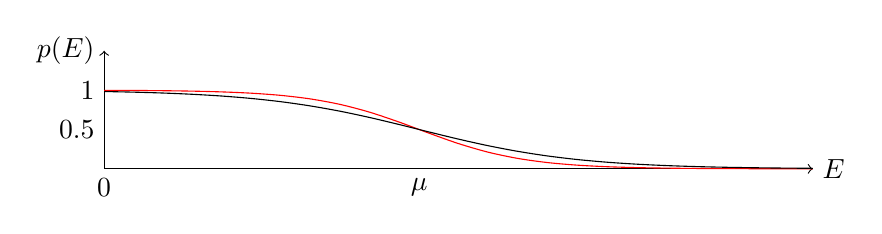
\begin{tikzpicture}
      \draw[->] (0,0) -- (9,0) node[right] {$E$};
      \draw[->] (0,0) -- (0,1.5) node[left] {$p(E)$};
      \draw[domain=0:9,smooth,variable=\x,red] plot ({\x},{1/(exp(1.5*(\x-4))+1)});
      \draw[domain=0:9,smooth,variable=\x,black] plot ({\x},{1/(exp((\x-4))+1)});
      \draw (0,0) node[below]{0};
      \draw (0,0.5) node[left]{$0.5$};
      \draw (4,0) node[below]{$\mu$};
      \draw (0,1) node[left]{$1$};
\end{tikzpicture}
\end{center}
\begin{Note}[Bulk Modulus in Metals]
Consider electrons in a box, as the box is compressed, the wavelengths of the wavefunctions shorten which increases the kinetic energy of the states increase, in turn increasing the total energy (since number of states do not change). there must be an outwards pressure. Given the ground-state energy $E$, one can calculate the pressure exerted by the electron gas from the relation $P=-(\frac{\partial E}{\partial V})_N$. Since $E=\frac{3}{5}NE_F$, where $E_F$ is proportional to $k_F^2$ which depends on $V$ via $n^{2/3}$. So 
$$P=-\frac{3}{5}N\frac{-2E_F}{3V}=\frac{2}{5}nE_F$$
The bulk modulus is then
$$B=-V\frac{\partial P}{\partial V}=-V\frac{\partial}{\partial V}\bigg(\frac{2NE_F}{5V}\bigg)=-\frac{2}{3}\frac{N}{V^2}E_F=\frac{2}{3}nE_F$$
since $E_F$ is proportional to $(N/V)^{2/3}$. 
\end{Note}
\begin{Note}[Heat Capacity of Metals]
Given the density of states $g(E)=\frac{m}{\hbar^2\pi^2}\frac{\sqrt{2mE}}{\hbar}$ for $E>0$ and 0 otherwise, the total internal energy density and number density is
$$U=\int_{-\infty}^{\infty}g(\epsilon)f(\epsilon)\epsilon d\epsilon,\quad N=\int_{-\infty}^{\infty}g(\epsilon)f(\epsilon)d\epsilon$$
Using the Sommerfeld expansion, (valid since only states within $\sim k_BT$ of the Fermi surface are able to absorb energy) we have
$$U\approx\int_0^{\epsilon_F}\epsilon g(\epsilon)d\epsilon+\epsilon_F(\mu-\epsilon_F)g(\epsilon_F)+\frac{\pi^2}{6}(k_BT)^2 \epsilon_F g'(\epsilon_F)+\frac{\pi^2}{6}k_B^2T^2g(\epsilon_F)$$
$$N\approx\int_0^{\epsilon_F} g(\epsilon)d\epsilon+\frac{\pi^2}{6}(k_BT)^2g'(\epsilon_F)+(\mu-\epsilon_F)g(\epsilon_F)$$
Since $n$ is independent of temperature, we have the second and third term sum to zero and hence $\mu=\epsilon_F(1-\frac{N^2k_B^2T^2}{12\epsilon_F^2})$. We thus have $U=U_0+\frac{\pi^2}{6}k_B^2T^2g(\epsilon_F)$ where $U_0$ is the energy density in the ground state. Since electrons are fermions, their particle number $N$ is conserved, so we have the heat capacity at constant volume to be
$$C_V=\bigg(\frac{\partial U}{\partial T}\bigg)_{N,V}=\frac{\pi^2}{3}k_B^2Tg(E_F)=\frac{\pi^2k_B^2TN}{2E_F}$$
Alternatively, we can use a more qualitative approximation. Only the electrons within $k_BT$ of the Fermi energy $E_F$ can be thermally activated, since the electrons deep in the Fermi sphere have no available states to excite to. There are a total of $g(E_F)k_BT$ number of these. Assume each electron has $\frac{3}{2}k_BT$ thermal energy, then the total electronic energy is
$$U_{el}=\frac{3}{2}k_BTg(E_F)k_BT$$
Since $N=\frac{V}{2\pi^2}(2m/\hbar^2)^{3/2}\int_0^{E_F}E^{1/2}dE$, $g(E_F)=\frac{V}{2\pi^2}(2m/\hbar^2)^{3/2}E_F^{1/2}=\frac{3N}{2E_F}$, and hence 
$$C_{el}=\frac{\partial U_{el}}{\partial T}\approx\frac{3N}{2k_BT_F}3k_B^2T=\frac{9Nk_BT}{2T_F}$$
One example where this approximation is in good agreement with experiment, is Sodium.
\end{Note}
\begin{Note}[Total heat capacity]
In general, both electrons and phonons contribute to heat capacity. We note that the phononic contributions completely dominate the specific heat at high temperatures. Well below the room temperature, their contribution falls off as $T^3$ (Debye's theory), and at very low temperatures it drops below the electronic contribution, which only decreases linearly with $T$ (electronic contribution dominates now), i.e. 
$$C_V=\gamma T+AT^3$$
where $\gamma\approx 1.67$ (in theory) and $A$ are constants. We note that there may be some discrepancy between theory and experiment due to electrons moving with an effective mass.
\end{Note}
\begin{Note}[Electrical Resistivity]
When an electric field is applied, the electrons start to move. Since they have extra momentum, the electron states are displaced in $k$-space. In the absence of scattering, the equation of motion is $\frac{d\mathbf{k}}{dt}=-\frac{e\mathbf{E}}{\hbar}$. In reality, electrons do not accelerate indefinitely since scattering processes occur to limit the displacement of the Fermi sphere.\\[5pt]
Phonons have a wavevector comparable to electrons, but the energies are tiny compared to $E_F$. Phonon scatterings can strongly change the direction of electron wavevector, but can only slightly change the magnitude. Defects can also produce large changes in the direction of $\mathbf{k}$, but only weak changes in energy.\\[5pt] There must be empty states available for scattering to occur. There are no free states within the body of the Fermi sphere. The only free states at similar energies to filled states are around the edge of the sphere, at the Fermi surface. The majority of electrons that are scattered are at the front of the Fermi sphere. The net result of scattering is that they are transferred to the back. The sphere reaches an equilibrium displacement in $k$-space, $\Delta k$, which corresponds to the drift velocity.
$$v_{drift}m^*=\hbar\Delta k$$
The scattering rate $\tau$ is an average of the electrons that are not scattered at all inside the sphere and those that are scattered strongly at the front. At high temperature, all phonon states are populated, so scattering by phonons is much more frequent than by defects, hence resistivity is proportional to temperature. At low temperatures, there are few phonons so defect scattering is dominant. Different samples have different defect densities, leading to temperature independent offset, known as the Matthiessens's rule.\\[5pt]
To compute electron thermal conductivity,
$$\kappa_{el}=\frac{1}{3}C_{el}\langle c\rangle\ell=\frac{1}{3}\frac{\pi^2nk_BT}{2T_F}v_F\tau=\frac{\pi^2nk_B^2T\tau}{3m^*}$$
At room temperatures, pure metals have $\kappa$ about 100 times that of insulators since electron thermal conductivity swamps phonon conductivity. At high temperature, phonons dominate scattering. Since $\tau\propto 1/T$, thermal conductivity is roughly constant with temperature.
\end{Note}
\begin{figure}[H]
    \centering
    \includegraphics[width=\linewidth, height=5cm]{scatteringfermisphere.PNG}
    \caption{Scattering occurs as the Fermi sphere is translated under an applied electric field}
\end{figure}

\begin{Note}[Evaluating Sommerfeld Model]
The Sommerfeld model can successfully explain
\begin{itemize}
    \item the temperature dependence and magnitude of electronic contribution to heat capacity;
    \item the approximate temperature dependence and magnitudes of the thermal and electrical conductivities of metals, and the Wiedemann-Franz ratio;
    \item the electronic magnetic susceptibility is temperature independent (additional example).
\end{itemize}
But it cannot explain
\begin{itemize}
    \item the Hall coefficients of many metals;
    \item the magnetoresistance exhibited by metals;
    \item other parameters such as the thermopower;
    \item the shapes of the Fermi surfaces in many metals;
    \item band structures (distinguish insulators and semiconductors from metals).
\end{itemize}
\end{Note}
\subsubsection*{Failures of the Free Electron Model}
\begin{Note}[Limitations of Free Electron Model]
Free electron model fail to explain:
\begin{itemize}
    \item The scattering length $\sim v_F\tau$ is about 100 Angstroms, but yet electrons do not scatter in metals. Why?
    \item Why do core electrons not count in the Fermi energy computation? What about insulators, which has no free electrons?
    \item Hall coefficient is still the wrong sign for some materials.
    \item Fail to account for the optical spectra (absorption intensity dependence on frequencies, as well as, colour).
    \item Measured specific heats are still off by factors as large as 10 for some metals.
    \item Electron-electron Coulomb interactions are roughly the same scale as the Fermi energy (Landau Fermi Liquid Theory)
\end{itemize}
\end{Note}
\newpage
\subsubsection*{Nearly Free Electron Model}
\begin{Note}[Nearly Free Electron Model]
In reality, electrons are not free, but are subjected to a potential, with periodicity of the underlying Bravais lattice, i.e. $U(\mathbf{r}+\mathbf{R})=U(\mathbf{r})$. Independent electrons, each of which obeys a one-electron Schr\"{o}dinger equation with a periodic potential, are known as Bloch electrons. 
\end{Note}
\begin{thm}[Bloch Theorem]
The eigenstates $\psi$ of the one-electron Hamiltonian $H=-\frac{\hbar^2}{2m}\nabla^2+U(\mathbf{r})$, where $U(\mathbf{r}+\mathbf{R})=U(\mathbf{r})$ $\forall\mathbf{R}$ in a Bravais lattice, can be chosen to have the form of a plane wave times a function with the periodicity of the Bravais lattice, i.e. $\psi_{nk}(\mathbf{r})=e^{i\mathbf{k}\cdot\mathbf{r}}u_{nk}(\mathbf{r})$, where $u_{nk}(\mathbf{r}+\mathbf{R})=u_{nk}(\mathbf{r})$ $\forall\mathbf{R}$ in the Bravais lattice.
\end{thm}
\begin{proof}
The Born-von Karman boundary conditions imposes the restriction $\psi(\mathbf{r}+N_i\mathbf{a_i})=\psi(\mathbf{r})$ where the $\mathbf{a_i}$ are the three primitive vectors and the $N_i$ are all integers of order $N^{1/3}$, where $N=N_1N_2N_3$ is the total number of primitive cells in the crystal. One can always expand any function obeying this condition in the set of all plane waves that all satisfy the condition, i.e. $\psi(\mathbf{r})=\sum_{\mathbf{q}}c_{\mathbf{q}}e^{i\mathbf{q}\cdot\mathbf{r}}$.\\[5pt]
Since the potential $U(\mathbf{r})$ is periodic in the lattice, its plane wave expansion will only contain plane waves with the periodicity of the lattice, and therefore with wavevectors that are vectors of the reciprocal lattice, $U(\mathbf{r})=\sum_\mathbf{K}U_\mathbf{K}e^{i\mathbf{K}\cdot\mathbf{r}}$. Since the potential is real, we require $U_{-\mathbf{K}}=U_{\mathbf{K}}^*$. If the crystal has inversion symmetry, then $U_{-\mathbf{K}}=U_{\mathbf{K}}$. We thus have
$$\bigg(\frac{\hbar^2q^2}{2m}-\epsilon\bigg)c_{\mathbf{q}}+\sum_{\mathbf{K'}}U_{\mathbf{K'}}c_{\mathbf{q}-\mathbf{K'}}=0$$
where since the plane waves satisfying the Born-von Karman boundary conditions are an orthogonal set, and hence each separate term must vanish. It is convenient to write $\mathbf{q}$ in the form $\mathbf{k}-\mathbf{K}$ where $\mathbf{K}$ is a reciprocal lattice vector chosen so that $\mathbf{k}$ lies in the first Brillouin zone. Further change of variables $K'\rightarrow K'-K$ yields
$$\bigg(\frac{\hbar^2}{2m}(\mathbf{k}-\mathbf{K})^2-\epsilon\bigg)c_{\mathbf{k-K}}+\sum_{\mathbf{K'}}U_{\mathbf{K'-K}}c_{\mathbf{k}-\mathbf{K'}}=0$$
For fixed $\mathbf{k}$ in the first Brillouin Zone, the set of equations $\forall\mathbf{K}$ couples only those coefficients $c_{\mathbf{k}},c_{\mathbf{k}-\mathbf{K}},c_{\mathbf{k}-\mathbf{K'}},...$ whose wavevectors differ from $k$ by a reciprocal lattice vector. We thus have $\psi_{\mathbf{k}}=\sum_{\mathbf{K}}c_{\mathbf{k}-\mathbf{K}}e^{i(\mathbf{k}-\mathbf{K})\cdot\mathbf{r}}$. This is of Bloch form with periodic function $u(\mathbf{r})=\sum_{\mathbf{K}}c_{\mathbf{k}-\mathbf{K}}e^{-i\mathbf{K}\cdot\mathbf{r}}$.
\end{proof}
\begin{Note}[Weak Periodic Potential]
There are two fundamental reasons why the strong interaction of the conduction electrons with each other and with the positive ions can have the net effect of a very weak potential.
\begin{enumerate}
    \item The electron-ion interaction is strongest at small separations, but the conducting electrons are forbidden from entering the immediate neighbourhood of the ions because this region is already occupied by the core electrons.
    \item In the region in which the conduction electrons are allowed, their mobility further diminishes the net potential any single electron experiences, for they can screen the fields of positively charged ions, diminishing the total effective potential.
\end{enumerate}
The matrix elements of this potential is
$$V_{k'-k}=\langle k|V|k\rangle=\frac{1}{L^3}\int e^{i(k-k')\cdot r}V(r)dr$$
which is zero unless $k'-k$ is a reciprocal lattice vector. Via perturbation theory, we see that $\epsilon_0(k)=\epsilon_0(k')$ corresponds to the degenerate situation, where $k'=k+G$. For 1D, we can see that $k'=-k=\frac{n\pi}{a}$, the Brillouin zone boundaries, is the only possible solution.\\[5pt]
If two plane wave states $|k\rangle$ and $|k'\rangle:=|k+G\rangle$ are of approximately the same energy, i.e. $k$ and $k'$ are close to zone boundaries, then we must diagonalize the matrix elements of these states first:
$$\langle k|H|k\rangle=\epsilon_0(k),\quad\langle k'|H|k'\rangle=\epsilon_0(k'),\quad\langle k'|H|k\rangle=V_G$$
Within this two-dimensional Hilbert space, we can write any wavefunction as a linear combination of $|k\rangle$ and $|k+G\rangle$. Using the variational principle to minimize the energy, i.e. equivalent to solving
$$\begin{bmatrix}\epsilon_0(k)&V_G^*\\V_G&\epsilon_0(k+G)\\\end{bmatrix}\begin{bmatrix}\alpha\\\beta\\\end{bmatrix}=E\begin{bmatrix}\alpha\\\beta\\\end{bmatrix}\implies(\epsilon_0(k)-E)(\epsilon_0(k+G)-E)-|V_G|^2=0$$
The simplest case is when $k$ is precisely on a zone boundary, i.e. likewise with $k'$. Hence, our characteristic equation simplifies to $E_{\pm}:=\epsilon_0(k)\pm|V_G|$. A gap opens up at the zone boundary, i.e. the two eigenstates form two linear combinations with energies split by $\pm|V_G|$.\\[5pt]
We next consider $k$ not quite on a zone boundary and for simplicity, we will stick to one dimension, i.e. $k=\frac{n\pi}{a}+\delta$ and this wavevector can scatter into $k'=-\frac{n\pi}{a}+\delta$ due to the periodic potential. We thus have $\epsilon_0(\pm\frac{n\pi}{a}+\delta)=\frac{\hbar^2}{2m}(\frac{n^2\pi^2}{a^2}\pm\frac{2n\pi\delta}{a}+\delta^2)$ and the characteristic equation simplifies to
$$E_{\pm}=\frac{\hbar^2}{2m}\bigg(\frac{n^2\pi^2}{a^2}+\delta^2\bigg)\pm\sqrt{\bigg(\frac{\hbar^22n\pi\delta}{2ma}\bigg)^2+|V_G|^2}\approx\frac{\hbar^2n^2\pi^2}{2ma^2}\pm|V_G|+\frac{\hbar^2\delta^2}{2m}\bigg(1\pm\frac{\hbar^2n^2\pi^2}{ma^2|V_G|}\bigg)$$
We can see that near the band gap at the Brillouin zone boundary, the dispersion is quadratic in $\delta$. Using the repeated zone scheme, we can see that small gaps open at the Brillouin zone boundaries in what is otherwise a parabolic spectrum. The corresponding effective mass is
$$m_{\pm}^*=\frac{m}{|1\pm\frac{\hbar^2n^2\pi^2}{ma^2|V_G|}}$$
where $E_{\pm}(G+\delta)=C_{\pm}\pm\frac{\hbar^2\delta^2}{2m^*_{\pm}}$.\\[5pt]
In general, near the Brillouin zone boundary, a gap opens up due to scattering by a reciprocal lattice vector. States of energy slightly higher than the zone boundary intersection point are pushed up in energy, whereas states of energy slightly lower than the zone boundary intersection point are pushed down in energy. The electronic spectrum breaks into bands, with forbidden energy gaps between the bands, i.e. these gaps are proportional to the periodic potential $|V_G|$.
\end{Note}
\begin{eg}[1D]
Let's consider a one-dimensional potential $V(x)=V_0\cos(\frac{2\pi x}{a})$. The Brillouin zone boundaries are at $k=\frac{\pi}{a}$ and $k'=-\frac{\pi}{a}$ so that $k'-k=G=-\frac{2\pi}{a}$ and $\epsilon_0(k)=\epsilon_0(k')$. The eigenstates are $|\psi_{\pm}\rangle=\frac{1}{\sqrt{2}}(|k\rangle\pm|k'\rangle)$. Writing the real space version of these $|k\rangle$ wavefunctions, we have $e^{ikx}$ and $e^{-ik'x}$ respectively. The two eigenstates $\psi_{\pm}$ are thus $\cos(\frac{\pi}{a}x)$ and $\sin(\frac{\pi}{a}x)$ respectively. The higher energy eigenstate $\psi_+$ has its density concentrated mainly at the maxima of the potential $V$ whereas the lower energy eigenstate $\psi_-$ has its density concentrated mainly at the minima of the potential.
\end{eg}
\begin{figure}[H]
    \centering
    \includegraphics[width=\linewidth]{nfem.PNG}
    \caption{Dispersion relation for nearly free electron model. Image credit: CMP notes by Cavendish.}
\end{figure}
\newpage
\subsubsection*{Band Structure~\cite{ashcroft1976solid,simon2013oxford,singleton2001band}}
\begin{Note}[Band Structure]
The number of $k$-states in a single Brillouin zone is equal to the number of unit cells in the entire system. Thus, if each unit cell has exactly 1 free electron, there would be exactly enough electrons to fill the band if there were only 1 spin state of the electron. Being that there are 2 spin states of the electron, when each unit cell has only 1 valence electron, the band is precisely half full. When a band is partially filled, the electrons can repopulate when a small electric field is applied, allowing current to flow. Hence, it is a metal.\\[5pt]
On the other hand, if there are 2 electrons per unit cell, then we have precisely enough electrons to fill 1 band. The entire lower band is filled and the upper band is empty, and there is a bandgap between the two bands. The lower filled band is the valence band and the upper empty band is the conduction band. At $T=0$ K, a sufficiently small electric perturbation will not create any excitation. Hence, they are insulators. If the bandgap is below 4eV, then they are semiconductors, since at room temperature, a few electrons can be thermally excited into the conduction band, and these electrons can move around freely, carrying some amount of current.
\end{Note}
\begin{eg}[Square Lattice and Filling of Brillouin Zone]
The number of electrons filling the Fermi circle in 2D is $N=2\frac{\pi k_F^2}{(2\pi/L)^2}=\frac{k_F^2L^2}{2\pi}$ where $L$ is the length of the 2D square lattice. Let $z$ be the number of valence electron per atom, $a$ is the lattice constant, then $k_F^2=\frac{2\pi N}{L^2}=\frac{2\pi z}{a^2}$.
Consider a square lattice of monovalent atoms, i.e. $z=1$. The Brillouin zone is correspondingly square, and since there is 1 electron per atom, there should be enough electrons to half fill a single Brillouin zone. In the absence of a periodic potential, the Fermi sea forms a circular disc, with an area precisely half the area of the zone, i.e. $\frac{1}{2}(\frac{2\pi}{a})^2=\pi k_F^2$. So the Fermi circle lies completely within the first Brillouin Zone, i.e. $k_F=\frac{\pi}{a}\sqrt{\frac{2}{\pi}}<\frac{\pi}{a}$ since $\pi>2\implies0<\frac{2}{\pi}<1$.\\[5pt]
When a periodic potential is added, gaps open up at the zone boundaries. This means that states close to the zone boundary get moved down in energy. Hence, states close to the boundary get filled up preferentially at the expense of states further from the boundary. This deforms the Fermi surface. If the periodic potential is strong enough the Fermi surface may even touch the Brillouin zone boundary. The Fermi surface continue to remain perfectly continuous since the Brillouin zone is periodic in $k$-space.\\[5pt]
Consider instead a square lattice of divalent atoms, i.e. $z=2$. For metals, in the absence of a periodic potential, the Fermi surface is still circular, although it now crosses into the second Brillouin zone. This is because now $k_F=\frac{\pi}{a}\sqrt{\frac{4}{\pi}}$ which is greater than $\frac{\pi}{a}$ since $\pi<4$. This is still less than $\frac{\sqrt{2}\pi}{a}$ (second Brillouin Zone). Note that because of this, the bands overlap such that the second zone can begin filling before the first is completely fill. However, states with wavevectors outside the first Brillouin Zone are not physical as, by Nyquist theorem, the $\lambda<a$ states fold-back into the first Brillouin Zone by subtracting an integer number of reciprocal lattice vectors.\\[5pt]
Again, when a periodic potential is added a gap opens at the zone boundary, pushing down the energy of all states within the first zone and pushes up energy of all states in the second zone. If the periodic potential is sufficiently strong, then the states in the first zone are all lower in energy than states in the second zone. Hence, the Fermi sea will have the entire lower band filled, and the upper band empty. For intermediate strength of potential, some states will remain occupied in the second zone, and some states will remain empty within the first zone.\\[5pt]
For insulators, there exists a sufficiently large bandgap at the zone boundary such that the energetically favourable configuration is to completely fill the first Brillouin Zone before starting on the second. So $k_F=\sqrt{2}\frac{\pi}{a}$.
\end{eg}
\begin{figure}[H]
    \centering
    \includegraphics[width=\linewidth]{squarelattice.PNG}
    \caption{(Left) Fermi sea of a square lattice
of monovalent atoms in 2D; (Centre and Right) Fermi sea of a square lattice of divalent atoms in 2D. \cite{simon2013oxford}}
\end{figure}
\begin{Note}[Bloch Oscillations]
If the electric field is strong and the scattering processes are weak, an extreme situation can be reached - occupied states move continuously through $k$-space. Strong electric field and weak scattering causes occupied states to steadily increase in $k$. The filled states cross into second Brillouin zone. The direction of electron group velocity reverses. Backfolding means the process is continuous. The group velocity and position of electrons oscillates.\\[5pt]
We can observe this in very pure samples at very low temperatures (4K), i.e. to reduce scattering. We create a huge unit cell in 1D (e.g. a superlattice of 34 layers of GaAs, then 6 layers of Al$_{0.3}$Ga$_{0.7}$As), hence a very small first Brillouin zone in $k$-space, hence allowing electron states to cross quickly. We apply a strong electric field, i.e. tetrahertz radiation (submillimetre wavelength) emitted at a frequency dependent on the electric field. We can also observe this in ultra cold Cesium atoms. The lattice is formed using optical standing wave. Lasers are used to push atoms with constant force. We can observe time dependence of momentum of the Cs atoms directly.
\end{Note}
\begin{figure}[H]
    \centering
    \includegraphics{blochoscillations.PNG}
    \caption{Illustration of Bloch Oscillation. Image credit: CMP notes from Cavendish.}
\end{figure}
\newpage
\begin{defi}[Effective Mass]
The effective mass is inversely proportional to the second derivative of $\epsilon(k)$, i.e. $m^*=\hbar^2/\frac{d^2\epsilon}{dk^2}$. The effective mass depends on bandstructure and particular band, and have different values at different $k$. Depending on the position of the Fermi energy $\epsilon_F$, more than one effective mass can contribute to conduction.
\end{defi}
\begin{Note}[Cyclotron resonance and holes]
In the presence of a magnetic field $\mathbf{B}$ pointing in the positive $z$-direction, the electron feels a  Lorentz force $-e\mathbf{v}\times\mathbf{B}$ which acts to deflect electrons in the negative $y$-direction. This force is orthogonal to the velocity and will act like a centripetal force that restricts these charge particles to follow circular trajectories. As such, a charged particle in a magnetic field moves in a helix along the magnetic field axis. The period $T$ of the circular motion depends on its mass $m$ and charge $e$,
$$T=\bigg|\frac{2\pi m}{eB}\bigg|$$
For particles in asymmetrical band structures, the particle no longer moves exactly in a helix, however its motion transverse to the magnetic field still moves in a closed loop (not necessarily a circle). Moreover, the time to complete one of these loops still varies inversely with magnetic field, and so it is possible to define a cyclotron effective mass $m=m^*$ from the measured period, using the above equation.\\[5pt]
The semiclassical motion of the particle can be described by a closed loop in k-space. Throughout this loop, the particle maintains a constant energy, as well as a constant momentum along the magnetic field axis. By defining $A$ to be the k-space area enclosed by this loop (this area depends on the energy $E$, the direction of the magnetic field, and the on-axis wavevector $k_B$), then it can be shown that the cyclotron effective mass depends on the band structure via the derivative of this area in energy:
$$m^*(E,\hat{B},k_{\hat{B}})=\frac{\hbar^2}{2\pi}\frac{\partial A(E,\hat{B},k_{\hat{B}})}{\partial E}$$
Typically, experiments that measure cyclotron motion (cyclotron resonance, de Haas–van Alphen effect, etc.) are restricted to only probe motion for energies near the Fermi level.\\[5pt]
In two-dimensional electron gases, the cyclotron effective mass is defined only for one magnetic field direction (perpendicular) and the out-of-plane wavevector drops out. The cyclotron effective mass therefore is only a function of energy, and it turns out to be exactly related to the density of states at that energy.\\[5pt]
Using cyclotron resonances, we can measure effective masses of `holes' as well, which are charged particles with a charge of the same magnitude but opposite sign. Suppose we start with an insulator or semiconductor and we excite one electron from the valence band to the conduction band. This excitation may be due to absorption of a photon, or it might be a thermal excitation. When the electron has been moved up to the conduction band, there is an absence of an electron in the valence band known as a hole. Since a completely filled band is inert, it is very convenient to only keep track of the few holes in the valence band and to treat these holes as individual elementary particles. The electron can fall back into the empty state that is the hole, emitting energy and annihilating both the electron and hole from the conduction and valence band respectively. 
\end{Note}
\newpage
\subsection{Semiconductors~\cite{simon2013oxford,singleton2001band}}
\subsubsection*{Theory}
\begin{Note}[Doping and Impurity States]
Doping refers to replacing a few of the semiconductor atoms, with valency 4, with impurity atoms of a different valence. These are extrinsic semiconductors.\\[5pt]
Imagine we replace one of the Si atoms in the lattice with P atom (with an extra proton and electron). Since the valence band is already filled, this additional electron must go into the conduction band. The P atom is known as a donor (or n-dopant) in Silicon since it donates an electron to the conduction band. Analogously, we can consider Al, which has one fewer electron than Si. Hence, Al is an electron acceptor (or p-dopant).\\[5pt]
When we add a single n-dopant to an otherwise intrinsic sample of Si, we get a single electron above the gap in the conduction band. The electron behaves like a free particle with effective mass $m_e^*$. Since we have a single extra positive charge $+e$ at some point in the crystal due to the P nucleus, the free electron is attracted back to this positive charge and forms a bound state.\\[5pt]
The two charges are attracted each other with a potential modified by the relative permittivity of the material $\epsilon_r$. Since the dielectric constant is typically high $\sim10$ and since $m^*$ is $\sim m_e/3$, the effective Rydberg constant is tiny compared to the real one. The effective Bohr radius can be huge compared to the real Bohr radius. Thus this donor impurity forms an energy eigenstate with energy just below the bottom of the conduction band. At zero temperature, this eigenstate will be filled, but it takes only a small temperature to excite a bound electron out of a hydrogenic orbital and into the conduction band, since the ionization energy is small (due to high dielectric constant and effective mass smaller than $m_e$).\\[5pt]
If the density of impurities is high enough, electrons or holes can hop from the impurity to the next, forming an impurity band. Since the effective Rydberg is very small, the impurity eigenstates are only slightly below the conduction band or above the valence band. With a small temperature, these donors or acceptors can be thermally excited into the band. Thus, except at low enough temperature that the impurities bind the carrier (carrier freeze out), one can think of the impurities as simply adding carriers to the band. Hence, the donor impurities donate free electrons to the conduction band, whereas the acceptor impurities give free holes to the valence band.\\[5pt]
In the absence of impurities, the Fermi energy ($\mu(T=0)$) is in the middle of the band gap. When the donor impurities are added, at zero temperature, impurity states near the top of the bandgap are filled. The Fermi energy is moved up to the top of the band gap. On the other hand, when acceptors are added, the acceptor states near the bottom of the band gap are empty. Thus the Fermi energy is moved down to the bottom of the bandgap.
\end{Note}
\begin{Note}[Occupation of the Bands]
The minimum energy of the conduction band and the maximum energy of the valence band are defined to be $\epsilon_c$ and $\epsilon_v$ respectively. The band gap is correspondingly $E_{gap}=\epsilon_c-\epsilon_v$. Recall that the density of states per unit volume for free electrons is
$$g(\epsilon\geq0)=\frac{(2m)^{1.5}}{2\pi^2\hbar^3}\sqrt{\epsilon}$$
The electrons in our conduction band are exactly like these free electrons, except that at the bottom of the band is at energy $\epsilon_c$ and have an effective mass $m_c^*$. The density of states for these electrons near the bottom of the conduction band and that for holes near the top of the valence band are respectively
$$g_c(\epsilon\geq\epsilon_c)=\frac{(2m_e^*)^{3/2}}{2\pi^2\hbar^3}\sqrt{\epsilon-\epsilon_c}$$
$$g_v(\epsilon\leq\epsilon_v)=\frac{(2m_h^*)^{3/2}}{2\pi^2\hbar^3}\sqrt{\epsilon_v-\epsilon}$$
If the chemical potential $\mu$ is well below the conduction band, i.e. $\beta(\epsilon-\mu)>>1$, then we can approximate $\frac{1}{e^{\beta(\epsilon-\mu)}+1}\approx e^{-\beta(\epsilon-\mu)}$ and so the Fermi statistics can be replaced by Boltzmann statistics. Hence, the density of electrons is
$$n(T)\approx\frac{(2m_e^*)^{3/2}}{2\pi^2\hbar^3}\int_{\epsilon_c}^\infty(\epsilon-\epsilon_c)^{0.5}e^{-\beta(\epsilon-\mu)}=\frac{(2m_e^*)^{3/2}}{2\pi^2\hbar^3}e^{-\beta(\epsilon-\mu)}\int_{\epsilon_c}^\infty(\epsilon-\epsilon_c)^{0.5}e^{-\beta(\epsilon-\epsilon_c)}=\frac{1}{4}\bigg(\frac{2m_e^*k_BT}{\pi\hbar^2}\bigg)^{3/2}e^{-\beta(\epsilon_c-\mu)}$$
where $\int_0^\infty x^{0.5}e^{-\beta x}dx=\frac{1}{2}\beta^{-3/2}\sqrt{\pi}$. Analogously, the density of holes is $\frac{1}{4}(\frac{2m_h^*k_BT}{\pi\hbar^2})^{3/2}e^{-\beta(-\epsilon_v+\mu)}$. The law of mass action is $n(T)p(T)=\frac{1}{2}\frac{k_B^3T^3}{\pi^3\hbar^6}(m_e^*m_h^*)^{3/2}e^{-\beta E_{gap}}$, which is independent of doping.\\[5pt]
For an intrinsic semiconductor, $p=n$ and so 
$$\mu=\frac{1}{2}(\epsilon_c+\epsilon_v)+\frac{3}{4}k_BT\lg(m_h^*/m_e^*)$$
Since $n=p$, by the law of mass action, $n_{intrinsic}=p_{intrinsic}=\sqrt{np}=\frac{1}{\sqrt{2}}(\frac{k_BT}{\pi\hbar^2})^{3/2}(m_e^*m_h^*)^{3/4}e^{-0.5\beta E_{gap}}$.
\end{Note}
\begin{figure}[H]
    \centering
    \includegraphics[width=\linewidth]{doping.PNG}
    \caption{Introduction of dopants create localized states in real space, but delocalized states in $k$-space. These energy levels are close to the present bands, dragging the chemical potential $\mu$ away from the midpoint. Image credit: CMP Notes by Cavendish.}
\end{figure}
\newpage
\subsubsection*{Applications}
\begin{Note}[P-N Junctions]
Although the n-doped system has free negatively charged electrons and the p-doped system has free positively charged holes, both systems are overall electrically neutral since charged ions compensate for the charges of the mobile charge carriers. When the two doped semiconductors are brought into contact, the electrons in the conduction band will fall into the valence band, filling the empty hole states, thus pair-annihilating both the electron and the hole. This amounts to a gain in energy of $E_{gap}$ per pair annihilated.\\[5pt]
After this process of electrons falling into holes and annihilating occurs there will be a region near the interface where there are no free carriers at all. This is the depletion region, which is electrically charged (since there are charged ions but no carriers to neutralize them). Hence, there is a net electric field pointing from the positively charged to the negatively charged ions.\\[5pt]
We now imagine moving an additional electron across the depletion region in order to annihilate another hole. While the annihilation process gives a gain in energy of $E_{gap}$, the process of moving the electron across the depletion region costs an energy of $-e\Delta\phi$, where $\phi$ is the electrostatic potential. When the depletion region is sufficiently large, it becomes no longer favorable for further electrons and holes to annihilate. 
\end{Note}
\begin{figure}[H]
    \centering
    \includegraphics[width=\linewidth]{pnjunction.PNG}
    \caption{Description of PN Junction. The drop in band energy is precisely compensated by the change in electrostatic potential. Image credit: CMP Notes by Cavendish.}
\end{figure}
\newpage
\begin{eg}[Rectification]
Rectification: allow current to flow through the junction easily in one direction, but not the other. There are 4 processes that can create current:
\begin{enumerate}
    \item Electrons may be thermally excited into the conduction band. Some of these electrons will flow down the slope to the left.
    \item Holes may be thermally excited down into the valence band and will flow up the slope to the right. 
    \item Electrons in the conduction band on the left will be thermally activated to climb up the potential slope in the depletion layer and will annihilate with holes once they arrive at the p-doped side. 
    \item Holes in the valence band on the right may be thermally activated to climb down the potential slope towards the n-doped side where they annihilate with electrons.
\end{enumerate}
The contribution by processes 1 and 2 to the current is directly proportional to $e^{-E_{gap}/k_BT}$. Voltage bias will not change the number of excited carriers, hence current independent of voltage.\\[5pt]
The contribution by processes 3 and 4 to the current is directly proportional to $e^{-E_{gap}/k_BT}$ in the absence of an applied voltage, and $e^{-(E_{gap}+eV)/k_BT}$ in the presence of an applied voltage. The total current flow will be the sum and hence
$$I=J_s(T)(e^{-eV/k_BT}-1)$$
where $J_s$ is directly proportional to $e^{-E_{gap}/k_BT}$ is known as the saturation current. This is the diode equation. Current flows easily in one direction, i.e. forward biased, but flows poorly in the opposite direction, i.e. reverse biased.
\end{eg}
\begin{figure}[H]
    \centering
    \includegraphics[width=\linewidth]{biasedPN.PNG}
    \caption{Band diagram of a biased p-n junction. The four processes that can create current are labelled. In the absence of applied voltage, the net current is zero. When voltage is applied, current flows easily for $eV<0$ and not easily with $eV>0$.~\cite{simon2013oxford} }
\end{figure}
\newpage
\begin{Note}[Direct and Indirect Band Transition]
If the value of $\mathbf{k}$ for the valence band maximum is the same as the value of $\mathbf{k}$ for the conduction band minimum, then we say that it is a direct bandgap. Otherwise if they differ, it is an indirect bandgap.\\[5pt]
Indirect transition may occur particularly if it is the minimum energy excitation. The electron is excited from the top of the valence band to the bottom of the conduction band at a very different $\mathbf{k}$. The momentum of the photon is extremely small so difficult to be spontaneously induced by photons alone (need conserve momentum). Many of times, it requires a phonon. Light emission is much less likely. Examples of the former is in GaAs and the latter is in Si.
\end{Note}
\begin{Note}[Breakdown under Reverse bias]
With sufficient reverse bias, a p-n junction can break down and conduct in the reverse direction. There are multiple mechanisms:
\begin{itemize}
    \item Zener breakdown is caused by tunneling at large reverse bias $\sim3V$. Large bias causes the energy at the top of the valence band in the p-type material to overlap the bottom of the conduction band in the n-type. Electrons can tunnel from the p-type to unoccupied states with the correct energy in the n-type. Heavy doping puts $\mu$ near the band edge and reduces the voltage needed for breakdown.
    \item Avalanche breakdown is caused by successive generation of carriers. Strong reverse bias is required. Thermally excited carriers within the junction gain energy between collisions, creating further electron-hole pairs, which gain energy and so form even more carriers. Large reverse current can flow. This dissipates a lot of heat and may damage the device.
\end{itemize}
Zener diodes are often used as a voltage reference in electronic circuits. Diodes designed to withstand avalanche breakdown can be used as voltage references, as protection devices, and even as single photon detectors (an incoming photon triggers the avalanche in a device held very near to that point).
\end{Note}
\begin{figure}[H]
    \centering
    \includegraphics[width=\linewidth]{semicon2.PNG}
    \caption{(Left): Direct versus Indirect transitions; (Centre) Zener breakdown; (Right) Avalanche breakdown. Image credit: CMP notes by Cavendish.}
\end{figure}
\begin{Note}[Light-Emitting Diode]
A light emitting diode is a p-n junction that is optimized for the production of photons during carrier recombination. To induce light emission, we forward bias the p-n junction. The majority of the carriers flow into the junction and recombine, releasing energy. In a direct bandgap material, light emission can be the most favourable process. The size of the bandgap determines the wavelength of the photons emitted. LEDs are widely used, including in communications and in efficient lighting. 
\end{Note}
\begin{Note}[Semiconductor Laser]
Population inversion occurs when higher energy states are more populated than lower energy states. Clearly, this is not at equilibrium, and needs to be continuously pumped. We need photon that matches energy levels, such that photon stimulates electron transitions, leading to further photon emission, hence the name Light Amplification by Stimulated Emission of Radiation.\\[5pt]
In a semiconductor laser, the population inversion is generated by electrical pumping, using a very large forward current. We need very heavy doping to place $\mu$ in the conduction and valence bands. We use a strong forward bias. Carriers are injected into the other side of the junction to maintain the population inversion.\\[5pt]
The junction is then surrounded by an optical cavity with partially reflecting surfaces to reflect photons backwards and forwards through the gain region. Some photons are transmitted at the interface, to form the laser beam. Semiconductor lasers are widely used in the telecommunications industry, as well as many other diverse applications.
\end{Note}
\begin{Note}[Solar Cells]
If one applies light to a semiconductor, electron-hole pairs may be excited if the energy of a photon is greater than the energy of the bandgap. In most regions of the semi-conductor, the created electrons and holes will quickly annihilate upon exposure to light. However, in the depletion region, due to the electric field in this region, electrons which are created flow off towards the n-doped region and holes which are created flow off towards the p-doped region. In both cases, the charge current is moving to the right.
\end{Note}
\begin{figure}[H]
    \centering
    \includegraphics[width=\linewidth]{semicon3.PNG}
    \caption{(Left): LED Diode; (Centre): Semiconductor Laser; (Right): Photovolatic Cell. Image credit: CMP notes by Cavendish.}
\end{figure}
\bibliographystyle{unsrt}
\bibliography{reference.bib}
\end{document}